\documentclass[a4paper]{article}
% ==== Inputs and Usepackages ====

\usepackage{tablefootnote}
\usepackage{enumerate}
\usepackage{float}
\usepackage{url}
\usepackage{hyperref}
\usepackage{dsfont}
\usepackage{mathrsfs}
\usepackage{amsmath}
\usepackage{amssymb}
\usepackage{amsthm}
\usepackage{amsfonts}
\usepackage{mathtools}
%\usepackage{mathabx}
\usepackage{MnSymbol}
\usepackage{xfrac}
\usepackage{nicefrac}
\usepackage{geometry}
\usepackage{graphicx}
\usepackage{graphics}
\usepackage{latexsym}
\usepackage{setspace}
\usepackage{tikz-cd}
\usepackage{tikz}
 \usetikzlibrary{matrix}
 \usetikzlibrary{calc}
 \usetikzlibrary{circuits.ee.IEC}
\usepackage{circuitikz}

\usepackage{a4wide}
\usepackage{fancybox}
\usepackage{fancyhdr}
\usepackage[utf8]{inputenc}




% ==== Page Settings ====

\hoffset = -1.2 in
\voffset = -0.3 in
\textwidth = 590pt
\textheight = 770pt
\setlength{\headheight}{20pt}
\setlength{\headwidth}{590pt}
\marginparwidth = 0 pt
\topmargin = -0.75 in
\setlength{\parindent}{0cm}


% ==== Presettings for files ====

\pagestyle{fancy}


\cfoot{\thepage}
\lfoot{\href{mailto:szekerb@student.ethz.ch}{szekerb@student.ethz.ch}}
\rfoot{Balázs Szekér, \today}
\lhead{Physics \uproman{3} Summary}


\title{Entrepreneurial Risk}
\author{Summary \\ \\ Balázs Szekér \\ szekerb@student.ethz.ch \\ \\
    Summary of the Lecture Entrepreneurial Risk \\
    in the Spring Semester 2021 given by Didier Sornette \\ \\
    Swiss Federal Institute of Technology, ETH Zürich}

\renewcommand{\abstractname}{Preface}
\fancypagestyle{myplain}
{
  \fancyhf{}
  \renewcommand\headrulewidth{0pt}
  \renewcommand\footrulewidth{0pt}
  \fancyfoot[C]{\thepage}
}

\theoremstyle{definition}

\newtheorem*{theorem}{Theorem}
\newtheorem*{definition}{Definition}
\newtheorem*{lemma}{Lemma}
\newtheorem*{proposition}{Proposition}
\newtheorem*{example}{Example}
\newtheorem*{corollary}{Corollary}

\begin{document}    

\begin{titlepage}
    \maketitle
    \thispagestyle{empty}
\end{titlepage}

\newpage
\pagenumbering{Roman}
\thispagestyle{myplain}
\begin{abstract}
    This is a summary of the topics dealt with in the lecture Entrepreneurial
    Risk in the spring semester 2021 given by Didier Sornette at ETH Zürich.
    This script is based on the lecture slides provided by Prof. Didier Sornette.
    All images and illustrations in this Script were taken from the lecture
    slides. The list of topics is not exhaustive. Many things were left out and
    only the topics which the author regarded as important are mentioned.
    This summary should neither be considered as a replacement of the lecture nor as
    a sufficient preparation for the exam. This summary should only be a reminder to
    which you can resort in case you quickly want to look something up.
    No liability is accepted in the event of failure to pass the examination.

    \vspace{1\baselineskip}

    If you stumble over mistakes, be it linguistic or thematic, or if you have suggestions
    what to add or how to improve this script, do not hesitate to contact me at
    szekerb@student.ethz.ch.

    \vspace{1\baselineskip}

    Many Thanks
    
    \vspace{1\baselineskip}

    Balázs Szekér
\end{abstract}

\newpage
\thispagestyle{myplain}
\tableofcontents

\newpage

\pagenumbering{arabic}

\section{Introduction}

\subsection{Entrepreneurship}

\begin{definition}[Entrepreneurship]

    \begin{itemize}
        \item Pursuit of opportunity without regard to resources controlled.
        \item Proceess of creating value through unique resource combinations
            that exploit opportunity.
        \item A way of thinking and acting, lot of different professional
            contexts, but also a way of approaching personal issues, family,
            life, community involvement, etc\dots
    \end{itemize}
\end{definition}

\begin{definition}[Success]
    
    \begin{enumerate}
        \item Know what you want in life. Know your end goals.
        \item Write down your intermediate goals and plan to reach these goals.
        \item Review and revise your plan monthly, keeping track of all setbacks
            and progess.
    \end{enumerate}
\end{definition}



\subsection{Risks}

\begin{quote}
    "Life is risk. Risk is life."
\end{quote}

\begin{definition}[Risk]
    \begin{itemize}
        \item A risk is a potential event with negative consequences that
            has not happened yet. However, a risk could also be defined as
            the event with unforeseen positive consequences.
        \item A possibility of Loss - Not the loss itself!
            \begin{itemize}
                \item A source of problem during a project
                \item Avoid labelling the cost of a risk as a risk. Find the source!
                \item Stike at the root of the problem, not the leaves!
            \end{itemize}
        \item Something that makes the project special.
            \begin{itemize}
                \item In the widest sense, everything is a risk.
            \end{itemize}
    \end{itemize}
\end{definition}

\paragraph{Types of Risk}
\begin{itemize}
    \item Industrial Risks
        \begin{itemize}
            \item Change in technology, productivity, prices
            \item false estimation of the rated capacity
            \item time needed for the construction and running-in periods,
                political, social and business environment
        \end{itemize}
    \item Operational Risk
        \begin{itemize}
            \item Lack of entrepreneurship skills.
            \item Poor unterstanding of market dynamics.
            \item Poorly available consultancy servises and information systems.
            \item Poof understanding of how to prepare a business plan.
            \item Natural risks.
        \end{itemize}
    \item Market Risks
        \begin{itemize}
            \item Unforeseeable inflation and exchange rates change.
            \item Customer behaviour to buy foreign gooods.
            \item Inadequate infrastructure.
            \item Shrinking market because of foreign competitors.
            \item Defaulting or insolvency, Credit risk.
        \end{itemize}
    \item Cultural risks
    \item Natural risks
    \item Economic and political risks
\end{itemize}

\begin{definition}[Hazard]
    A hazard is an act or phenomenon posing potential harm to some person(s)
    or thing(s), i.e. a source of harm, and its potential consequences.
    Hazards need to be identified and considered in projects' lifecycle analyses
    since they could pose threat and could lead to project failures.
\end{definition}

\begin{definition}[Unknown Unknown]
    A type of uncertainty in which you do not know that this uncertainty
    even exists.
\end{definition}

\begin{definition}[Risk assessment]
    Risk assessment consists of: Hazard identification, Event probability
    assessment and Consequence assessment.
\end{definition}

\begin{definition}[Risk Control]
    Risk control require the definition of acceptable and comparative evaluation
    through monitoring and decision analysis. Risk control also includes
    failure prevention and consequence mitigation. 
\end{definition}

\begin{definition}[Risk Communication]
    Risk communication involves perceptions of risk and depends on the
    audience targeted. Hence, it is classified into Risk communication
    to the media, to the public and to the engineering community.
\end{definition}

\begin{definition}[Human Errors]
    Human errors are unwanted circtumstances caused by humans that result
    in deviations from expected norms that place systems at risk.
    It is important to identify the relevant errors to make accurate risk
    asssessment. Human error identification techniques should provide a
    comprehensive structure for determining significant human errors within
    the system.
    \begin{itemize}
        \item \underline{Human error Modelling}: Currently, there is no
            consensus on how to model humans reliably. The human error
            rate estimates are often based on simulation tests, models,
            and expert estimation.
        \item \underline{Human Error Quantification}: Still a developing
            science requiring understanding of human performance, cognitive
            processing, and human perceptions.
    \end{itemize}
\end{definition}


\pagebreak

\section{Setting the landscape on entrepreneurship and private investment}

\begin{figure}[h]
    \centering
    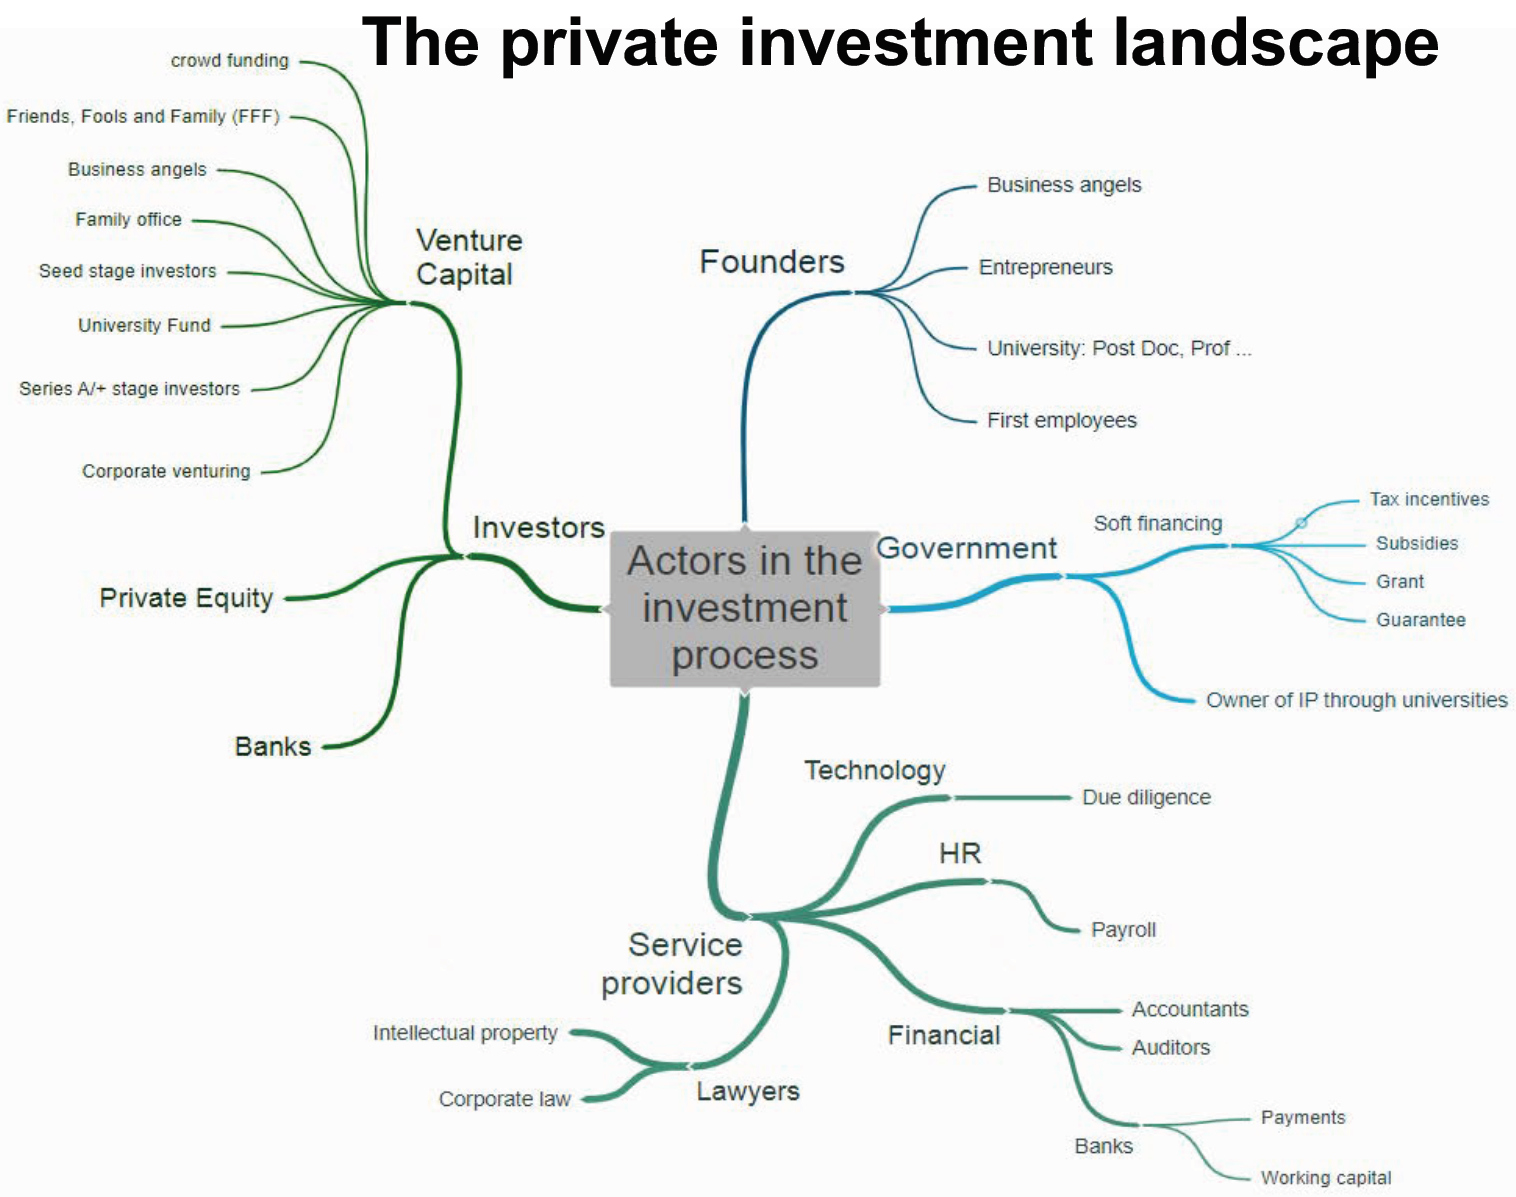
\includegraphics[width=0.8\textwidth]{Pictures/private_investment_landscape.png}
    \caption{Private investment landscape}
    \label{private_investment_landscape}
\end{figure}


\paragraph{Difference between Private Equity and Venture Capital}

\begin{definition}[Private equity]
    \begin{itemize}
        \item Financing mainly used to buy mature well-established companies
        \item and get full control (100\% of company)
        \item Always a combination of debt and equity (shares)
        \item Calue created through streamlining of operations, cost cutting, consolidation\dots
        \item Strong fucus on cash flow to pay of debt, companies are highly leveraged (much debt relative to equity)
        \item Leverage increases risk profile but also potential returns.
        \item Large deal sizes (hundreds of millions)
    \end{itemize}
\end{definition}

\begin{definition}[Venture capital]
    \begin{itemize}
        \item Financing mainly given to startup companies and small businesses
        \item Value created through growth
        \item Growth expected from innovation, disruptive technology, new product, business plan
        \item Very high risk profile, no cash flow but cash burn (that is where the money is used for)
        \item Company can only finance through equity, often risk profile is too high to get debt financing
        \item Smaller deal sizes (millions)
        \item No full control (50\% or less)
    \end{itemize}
\end{definition}

\begin{definition}[Asset and leverage]
    \begin{align*}
        \text{Asset} = \text{Debt} + \text{Equity}
        \hspace{10pt} , \hspace{10pt}
        \text{Leverage} = \frac{\text{Asset}}{\text{Equity}} = \frac{\text{Debt}}{\text{Equity}} + 1
    \end{align*}
\end{definition}

Most new businesses do not survive the first five years.
Investors want to manage their risk with preference shares and by gaining as much
control as possible on the company, through shareholder agreements, voting rights,
board membership, anti-dilution clauses\dots

\paragraph{Liquidation preferences}
\begin{itemize}
    \item Much VCs invest using so-called 'preference shares' instead of common shares.
    \item In the event of the failure of the company, preferred shareholders may receive payment from liquidation before common shareholders.
    \item When the company is sold (at the so-called exit), preferred shareholders may receive
        payment (sometimes with a guaranteed ROI) in full before the common shareholders.
\end{itemize}

The pay-off is highly skewed, many loosers and a few big winners.
Investors must be detached from individual companies and look at the whole
portfolio. This is not aligned with the Entrepreneurs' viewpoint.

\vspace{1\baselineskip}

Risk and return are like Yin and Yang

\begin{figure}[h]
    \centering
    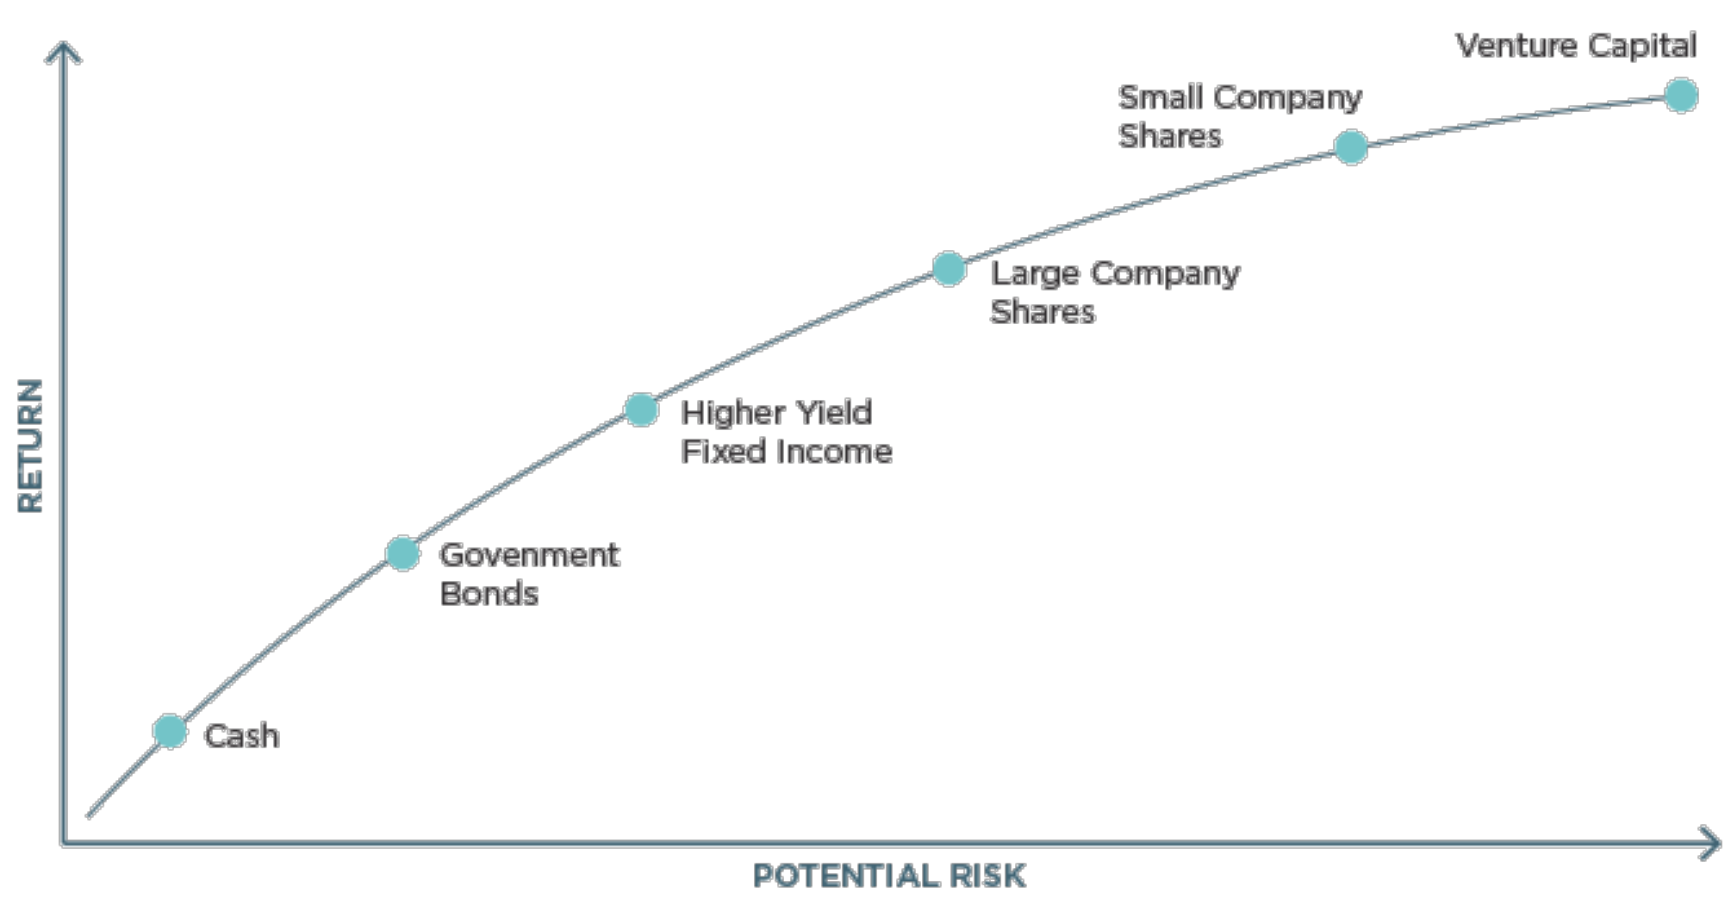
\includegraphics[width=0.5\textwidth]{Pictures/potential_risk_return_graph.png}
\end{figure}

\paragraph{Perceived vs. actual risk}
Two kinds of bias were identified: (a) a tendency to overestimate small frequencies
and underestimate larger ones; and (b) a tendency to exaggerate the frequency of
some specific causes and to underestimate the frequency of other, at any given level
of objective frequency.

\paragraph{Prospect Theory: Kahnman and Tversky}
"Losses loom larger than gains." Individuals assess losses and gains in an
asymmetric way e.g. for some people, the pain from losing 1000 USD could
only be compensated by the pleasure of earning 2000 USD.

\paragraph{Viewpoints of Investors and Entrepreneurs} \

\begin{figure}[h]
    \centering
    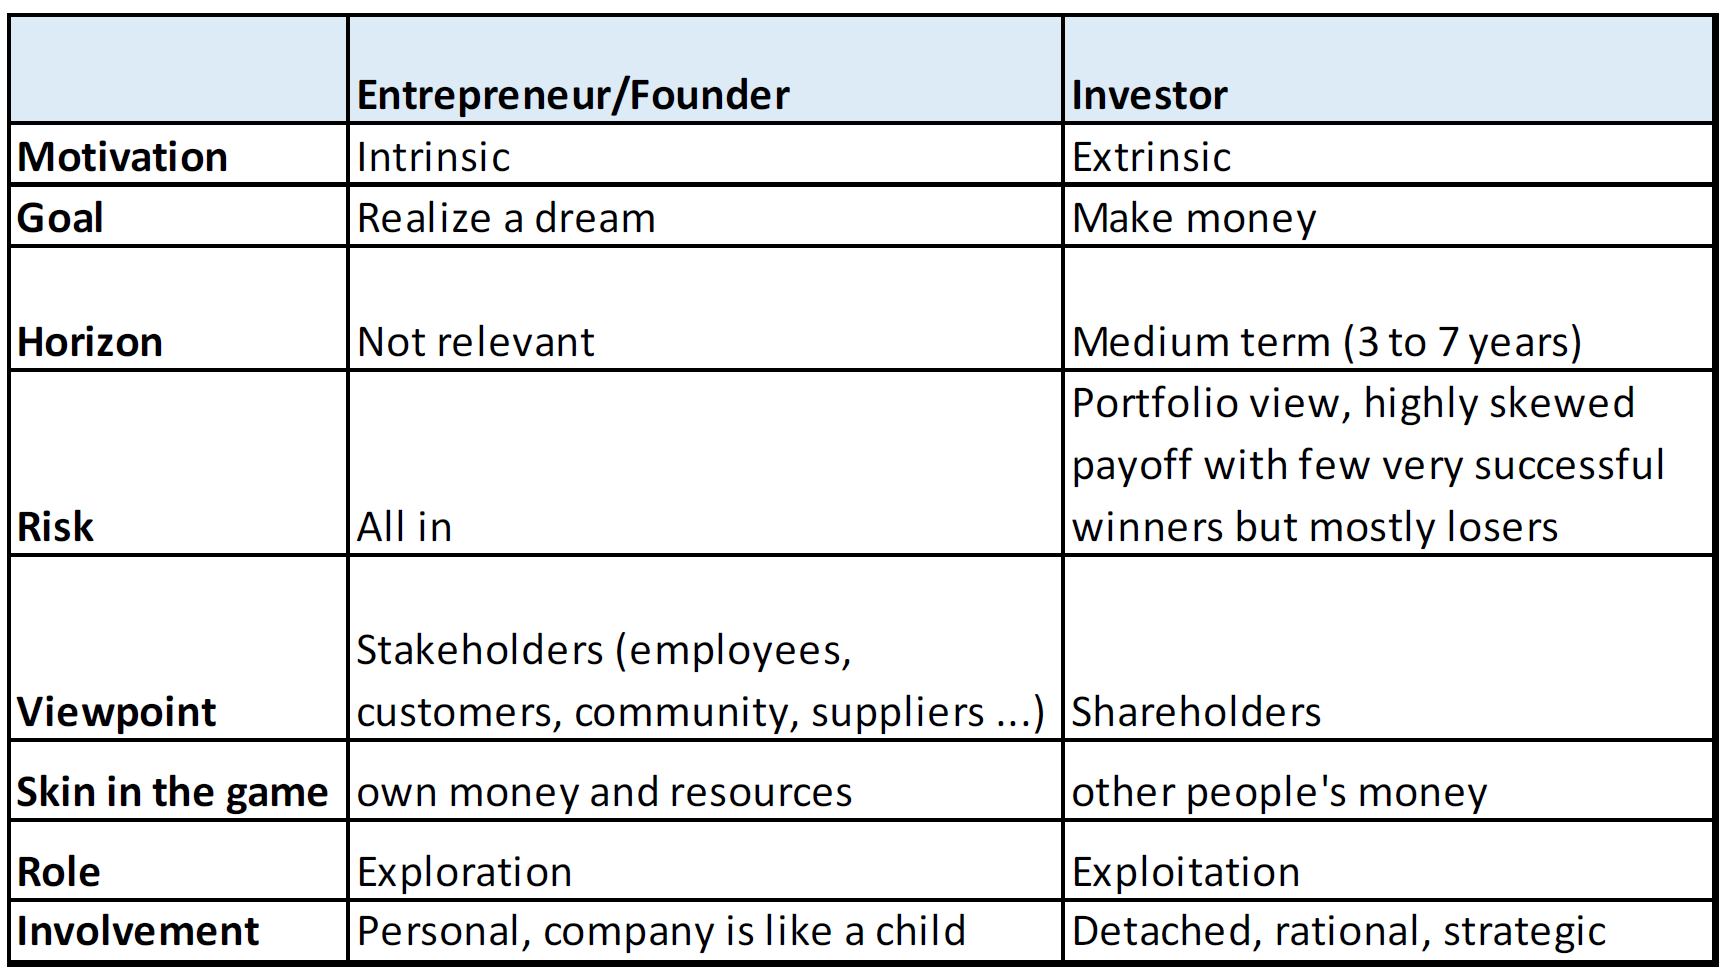
\includegraphics[width=0.5\textwidth]{Pictures/viewpoints_entrepreneurs_investors.png}
\end{figure}

\paragraph{Challenges of exploration}
According to Herbert Simon exploration requires:
\begin{itemize}
    \item tolerance of ambiguity/uncharted territory
    \item patience: learning-by-doing, accumulation of knowledge, trial-and-error
    \item luck / serendipity
    \item persistence / diligence
    \item 'intuition': use of smart heuristics
\end{itemize}
It is a high risk endeavor, where the payoff is almost impossible to estimate.

\paragraph{Exploitation}
Exploitation is tempting from a short-term risk/return perspective, but there are
serious caveats on the long run.

\begin{figure}[h]
    \centering
    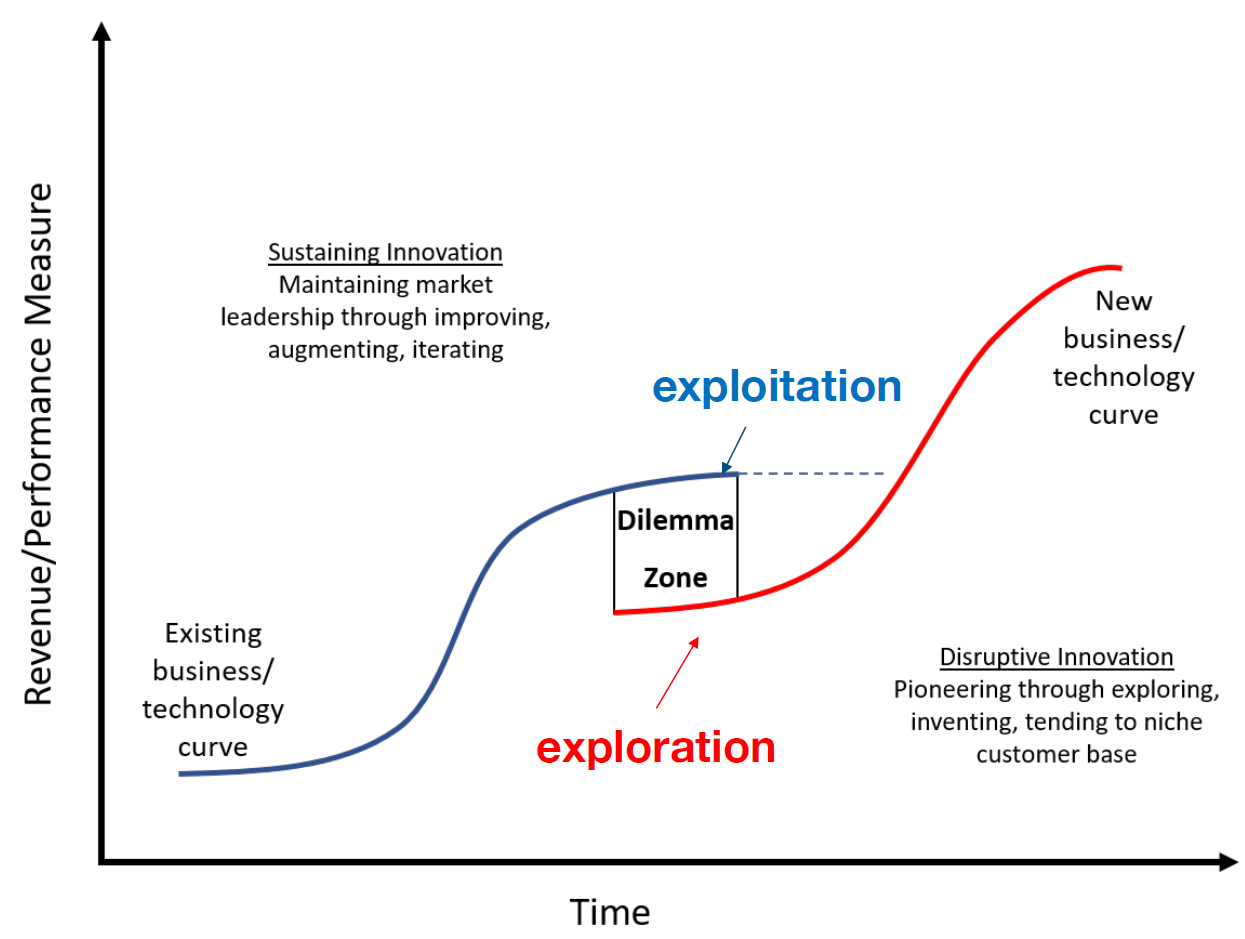
\includegraphics[width=0.5\textwidth]{Pictures/exploration_exploitation_curve.png}
\end{figure}

Disruptive innovations are initially too small to meet the ROI-targets of large
established firms. However, they steadily work their way up eventually
capitalizing on a crucial first mover advantage against large, less nimble,
market leaders.

\paragraph{Important Terms}
\begin{itemize}
    \item Regression to the mean
    \item Narrow Framing
\end{itemize}

\paragraph{How to deal with biases?}
\begin{itemize}
    \item \underline{Heuristics}: When predictability is poor, inconsistency,
        based on unnoticed stimuli, is destructive of any predictive validity.
        Be consistent by using investment criteria, simple formular, recipies
        or rules of thumb.
    \item \underline{Example, consider an outside view}: Prior to the use of any
        inside information, try to predict a totally independent base rate e.g.
        "how many start-ups in this field survive the first three years?"
        Use this as your anchor and adjust this base rate according to information
        obtained during the due diligence.
    \item \underline{Decorrelate error}: Ask people's opinion indepentently of each
        other, wisdom of crowds vs. group think, practice "constructive confrontation",
        avoid "cozy unanimity"
    \item \underline{Sunk Cost}: Be aware of the difficulty to take a loss. A new
        manager does not carry the same mental accounts and is therefore more
        able to ignore the sunk of past investments.
    \item \underline{Validity of intuition}: Intuition cannot be trusted in the
        absence of stable regularities in the environment and in the absence of
        prolonged practice and learning.
\end{itemize}

\paragraph{Closing a deal}
Only a fraction (0.5-2\%) of considered deals get closed.

\begin{figure}[h]
    \centering
    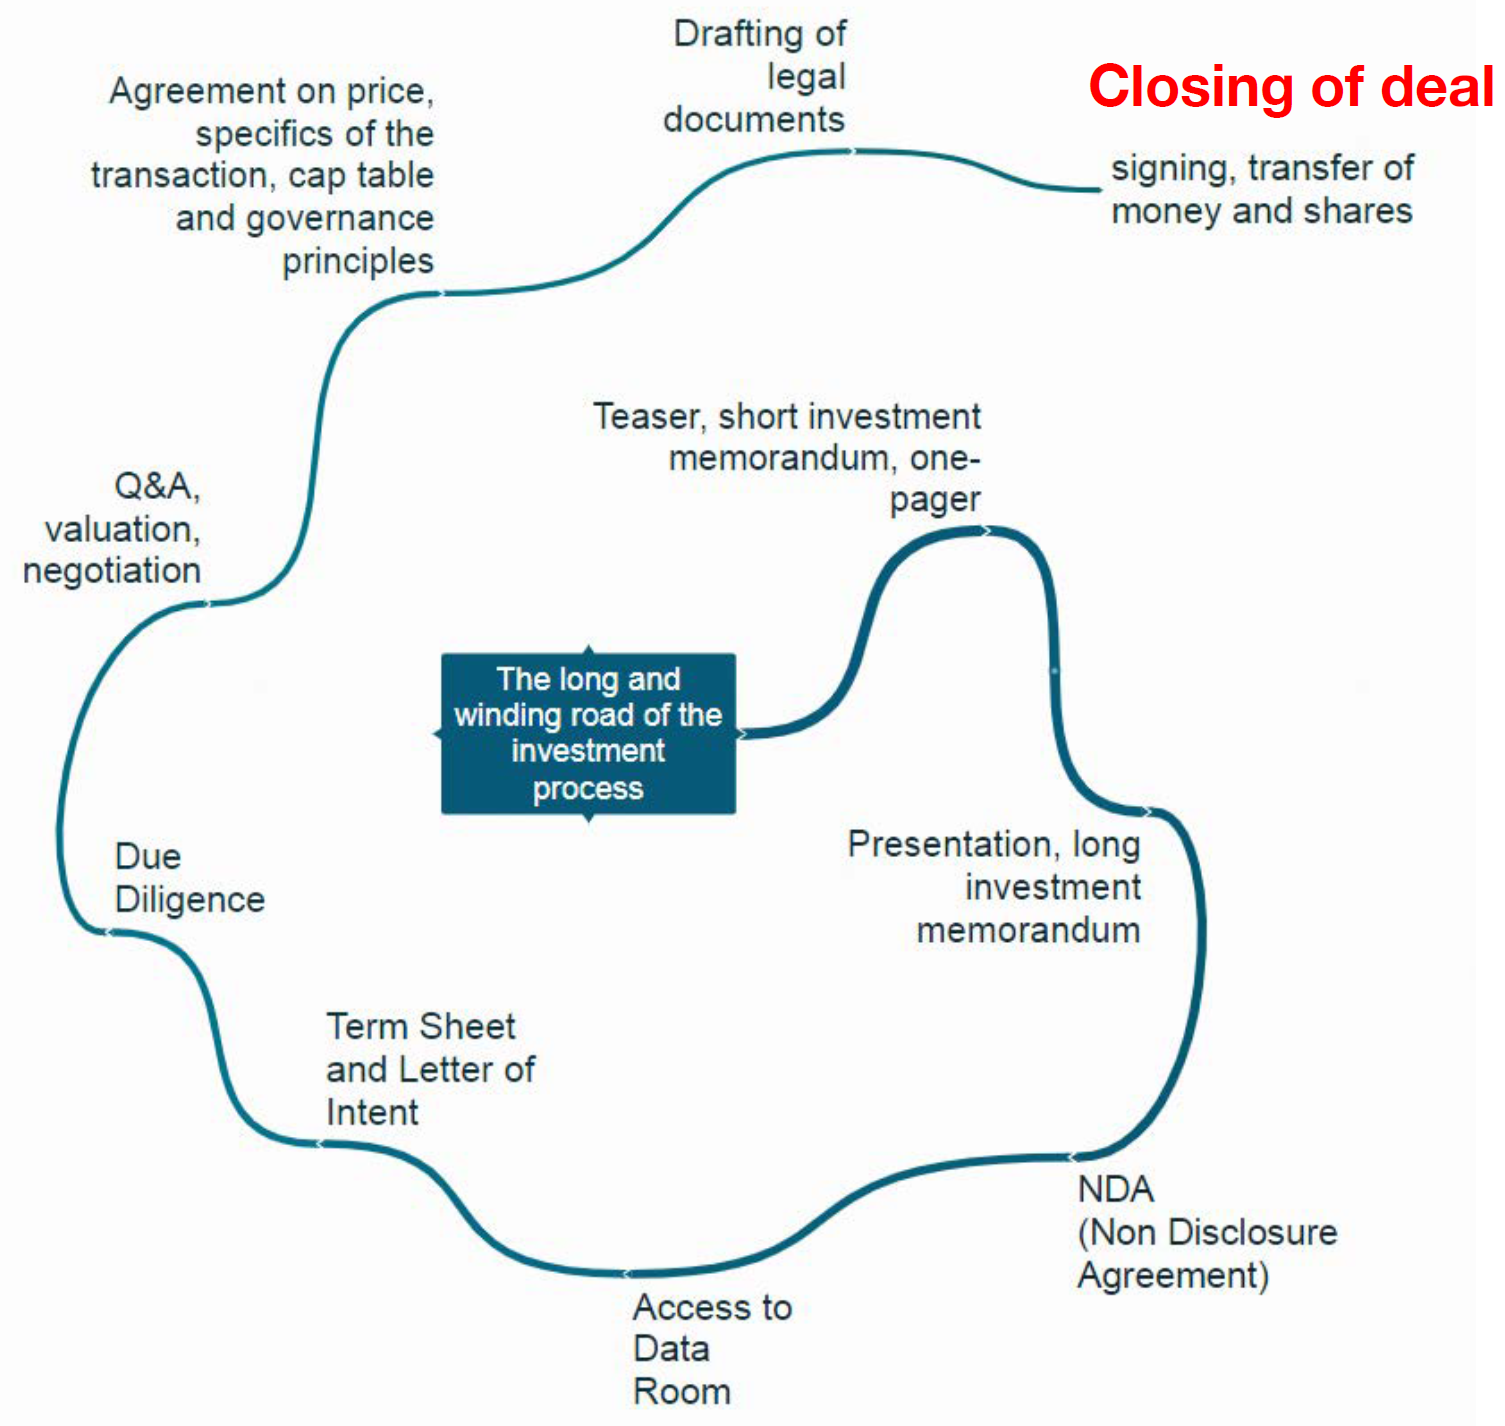
\includegraphics[width=0.45\textwidth]{Pictures/closing_Deal.png}
\end{figure}

\paragraph{Pitch Deck}
\begin{itemize}
    \item Sales pipeline, proven market interest, test by the market\dots
    \item Growth strategy: sales, product development, scalability, BOM
    \item Investment: Use of proceeds
    \item Current cap table
    \item Exit options for investor
\end{itemize}

\begin{figure}[h]
    \centering
    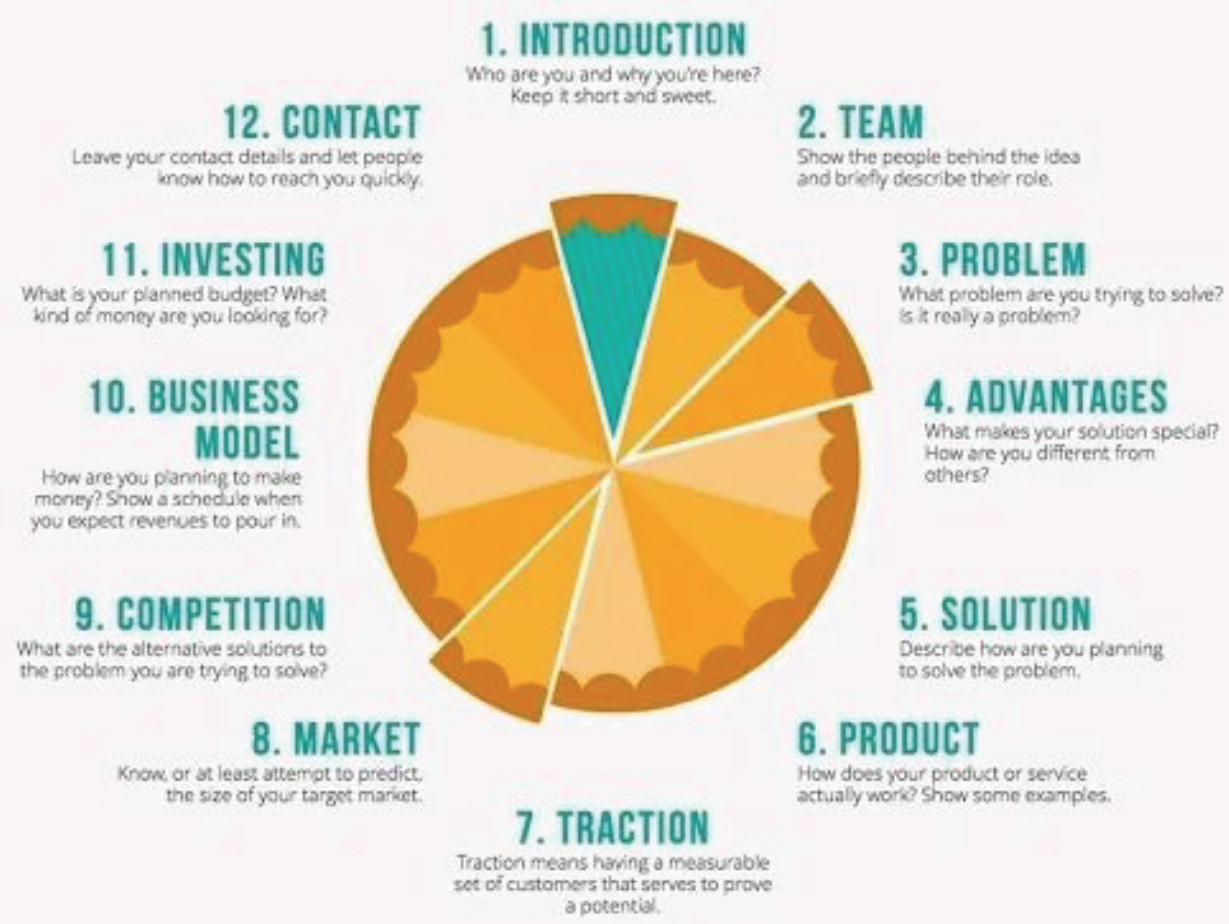
\includegraphics[width=0.8\textwidth]{Pictures/12_slides_of_a_pitch_deck.png}
    \caption{Pitch Deck}
\end{figure}

\paragraph{Get to know each other}
Possible Questions:
\begin{itemize}
    \item Team:
        \begin{itemize}
            \item Does your company culture and values math with us?
            \item Are there complementary skills in your core team?
            \item Can you give references for your key employees? 
        \end{itemize}
    \item Technology:
        \begin{itemize}
            \item What makes your technology unique?
            \item How is the Intellectual Property proteted?
        \end{itemize}
    \item Product:
        \begin{itemize}
            \item Is it developed beyond the design phase?
            \item How does it scale?
            \item How does your bill of materials (BOM) change with production volumes?
        \end{itemize}
    \item Market:
        \begin{itemize}
            \item Do you understand the market?
            \item How do you plan to access the market?
            \item How big is the market?
            \item What market share are you targeting?
        \end{itemize}
    \item Sales:
        \begin{itemize}
            \item Describe your customer. Can you give references?
            \item What are their problems and how do your provide solutions?
            \item How are your sales distributed over the customers?
            \item What kind of sales process do you have? Direct vs distributed sales?
                Do you have salespeople with experience, a trustworthy pipeline, good lead customers?
            \item Do you have a ROI model for your client, or do you deliver a nice-to-have product?
        \end{itemize}
    \item Economics:
        \begin{itemize}
            \item Do you understand the big trends?
            \item Does your product serve a long-term goal, service a need?
            \item How does your product fit the big changing trands?
        \end{itemize}
    \item Financials:
        \begin{itemize}
            \item Do you have a storng and robust business plan?
            \item Do you understand you future cash flow?
            \item Do you understand the risks?
            \item What are the sensitivities? Worst case scenario?
            \item Do you have a fallback/plan-B?
        \end{itemize}
\end{itemize}


Also ask the investors what their interests and terms are.

\paragraph{NDA - Non-Disclosure Agreement}

If the introduction round is finished successfully a Non-Disclosure Agreement (NDA)
is signed between the investor and the founders. This is a legal contract that outlines
the use of confidential material, knowledge and information that the parties wish
to exchange. After the NDA is signed by both parties, access is given to the data
room.

\paragraph{Term sheet / Letter of Intent}
After a first check of the data room, the investors will produce a term sheet or
LOI, this outlines an agreement that two or more parties exept to make. Term
sheet and LOI are very similar in content, but TS is structured as a list, often
in a table format, whereas LOI is in the form of a letter. Written before the
execution of a formal and binding contract, most of the listed agreements are
not legally binding.
Topics are:
\begin{itemize}
    \item Valuation of the company
    \item Amount of investment
    \item Use of proceeds
    \item Cap table
    \item Share preferences
    \item Governance (Board composition and chair)
    \item Investor commitment
    \item Management commitment
    \item Exit (right of first refusal)
    \item Description of the Due Diligence process (time, topics,\dots)
    \item Exclusivity
\end{itemize}

\paragraph{Exclusivity}
Legal binding clause of the LOI or TS. Caveat: Transfers a lot of control to
the investor, he/she will be the only party taking the next step in the process,
he/she can take advantage of the 'sunk cost effect', often exclusivity periods
are extended. When giving exclusivity, time is on the side of the investor.
The investor can put you under pressure, test your tenacity and patience, try
to decrease the valuation of the company. When you give exclusivity, you cancle
out any competition for the investor, this will make him/her dominant.

\paragraph{Due diligence}
After the Term Sheet and/or the Letter of Intent are signed, the Due Diligence
process is started. This is supposed to take only up to six weeks, in reality,
it will turn out to be many months. Now, the external advisors enter the arena.
\begin{itemize}
    \item \underline{Business lawyers}: will examine all the contracts in the data room.
    \item \underline{IP lawyers}: will study the strengths of the patents of the company
        and the 'freedom to operate'
    \item \underline{External auditor}: will validate the accounting, finance statements,
        balance sheet, taxes
    \item \underline{Technological consultant}: may analyze the product development
        and the strength and relevance of the technology with respect to other solutions.
\end{itemize}
Investors themselves will:
\begin{itemize}
    \item Do reference checks of clients, founders, key personal.
    \item Analyze the commercial viability of the product and the sales process
        and tools.
    \item Study the quality of the sales pipeline.
    \item Based on that will make their own forecast of future sales.
    \item And a forecast of future cashflows.
\end{itemize} 
Based on the results of the due diligence, the investors will challenge the
business plan. This will allow them to:
\begin{itemize}
    \item Create base-case and worst-case scenarios of cash burn
    \item Check the investment amount and the use of proceeds with respect to these
        scenarios, are the founders asking too much, too little?
    \item Assess the risk of their investment.
    \item Set goals, milestones for the Management
    \item Find the gaps, see where the company needs further support
    \item Check, whether some of these gaps are a no-go
    \item Possibly discuss releasing the invested amount in tranches, each time
        when a certain milestone is reached.
    \item Make their own valuation of the company.
\end{itemize}


\pagebreak

\section{Introduction to company valuation}

There are three key financial statements: the balance sheet, the income statement
and the statement of cash flow. We will give three approaches towarts valuation:
\begin{itemize}
    \item Balance sheet: Static/snapshot: Equity = Assets - Liabilities
    \item P\&L: Relative value: using multiples and metrics from the Profit and
        Loss account (net income, EBITDA, EBIT)
    \item Discounted cash flow: Absolute value: using the cash flows that will be
        generated by the business to calculate the Net Present Value of the business
        - like the valuation of a bond.
\end{itemize}

\subsection{Balance Sheet}

\paragraph{Enterprise Value}
is the price to acquire the whole company, the shares, the debt but also
receiving the cash. EV = Equity + Debt - Cash

\paragraph{Equity Value}
is the price to acquire only the shares of a company.

\vspace{1\baselineskip}

EV valuation will give you the price to take over the whole business including cash
and debt, Equity will give you the price to buy the shares.

\paragraph{Tangible vs. Intangible Assets}
Tangible Assets are: Cash, Furniture, Plant and Machinery, Vehicles,
Building, Stock, Equipment, Computers,\dots

Intangible Assets are: Patents, Logo, Copyright, Brand Value, Self-developed
softwares, customer data, Trademark, Goodwill.

\paragraph{Taxi example} See Lecture from 10.03.2021

\begin{figure}[h]
    \centering
    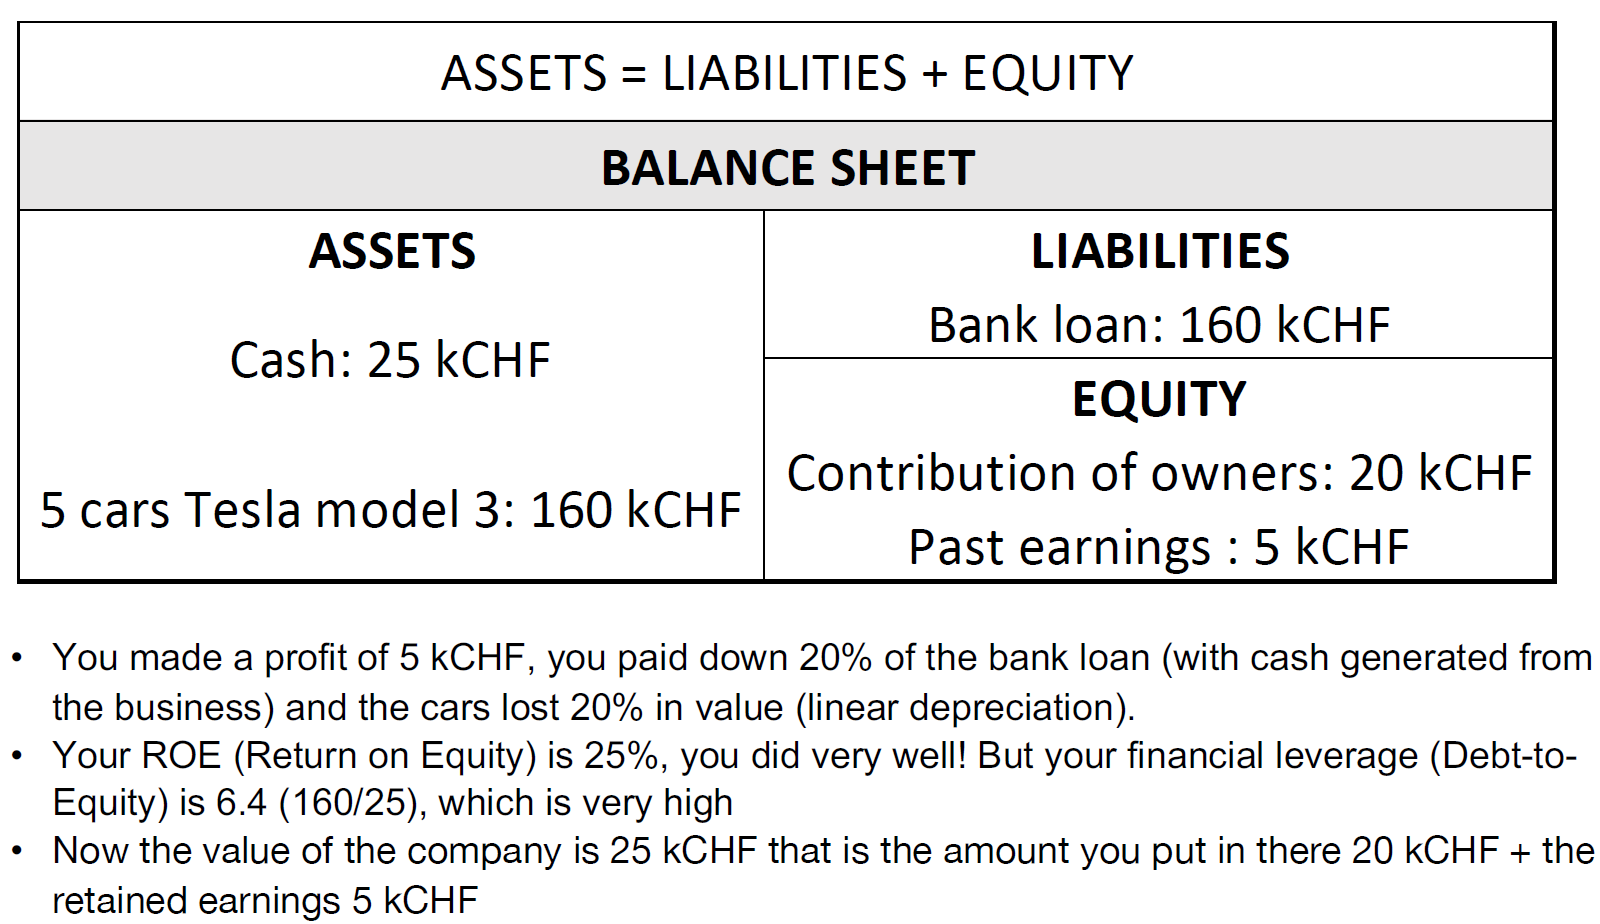
\includegraphics[width=0.5\textwidth]{Pictures/Taxi_example.png}
\end{figure}

However, leverage increases your risk proportionally.

\paragraph{Banking}
Before the financial crisis in 2007/2008 Banks had really high leverage.
It can lead to a domino effect: if one big bank goes bank rupt, others may
suffer as well resulting in the economy to collaps.

\subsection{P \& L - Profit and Loss}

\paragraph{Income Statement}
A Profit and Loss statement, or also called Income statement, summarizes the
revenues, costs and expenses incurred during a specified period, usually a fiscal
quarter or year. It provides information about a company's ability or inability
to generate profit by increasing revenue, reducing costs or both.

\paragraph{Different Components of P \& L}
\begin{itemize}
    \item \underline{Revenues (sales)} = income per hour * operating hours per
        year * occupancy rate * fleet size
    \item \underline{Costs of goods sold} = cost of the material and labor directly
        used to run the business. COGS = operating hours per year * fleet size *
        (costs per hour for the driver + operating costs * occupancy rate)
    \item \underline{Gross Margin} = Revenue - COGS
    \item \underline{OPEX} = Operating Expenses (the remaining costs that are not 
        included in COGS)
    \item \underline{EBIT} = Earnings Before Interest and Taxes (Operating Profit)
        = Gross Margin - OPEX
    \item \underline{EBITDA} = Earnings Before Interest, Taxes, Depreciation and
        Amortization = EBIT + D\&A
    \item \underline{EBT} = Earnings Before Taxes = EBIT - Interest paid
    \item \underline{Net Profit} = EBIT - Interest paid - taxes
\end{itemize}

A company is a 'process'.

\paragraph{Relative valuation and the use of multiples}
In relative valuation, the value of an asset is deduced from the market value
of a set of similar assets. To do relative valuation we need to identify comparable
assets and obtain their market value and standardize these market values, because
absolute prices cannot be compared. This process of standardization creates
price multiples.

\paragraph{Valuation multiples}
\begin{itemize}
    \item \underline{P/E ratio}: Calculate a company's share price (Equity)
        from its earnings (net profit).
    \item \underline{EV/EBITDA ratio}: Calculate a company's Enterprise Value
        from its EBITDA.
    \item \underline{EV/EBIT ratio}: Calculate a company's Enterprise value
        from its EBIT.
\end{itemize}

\begin{figure}[h]
    \centering
    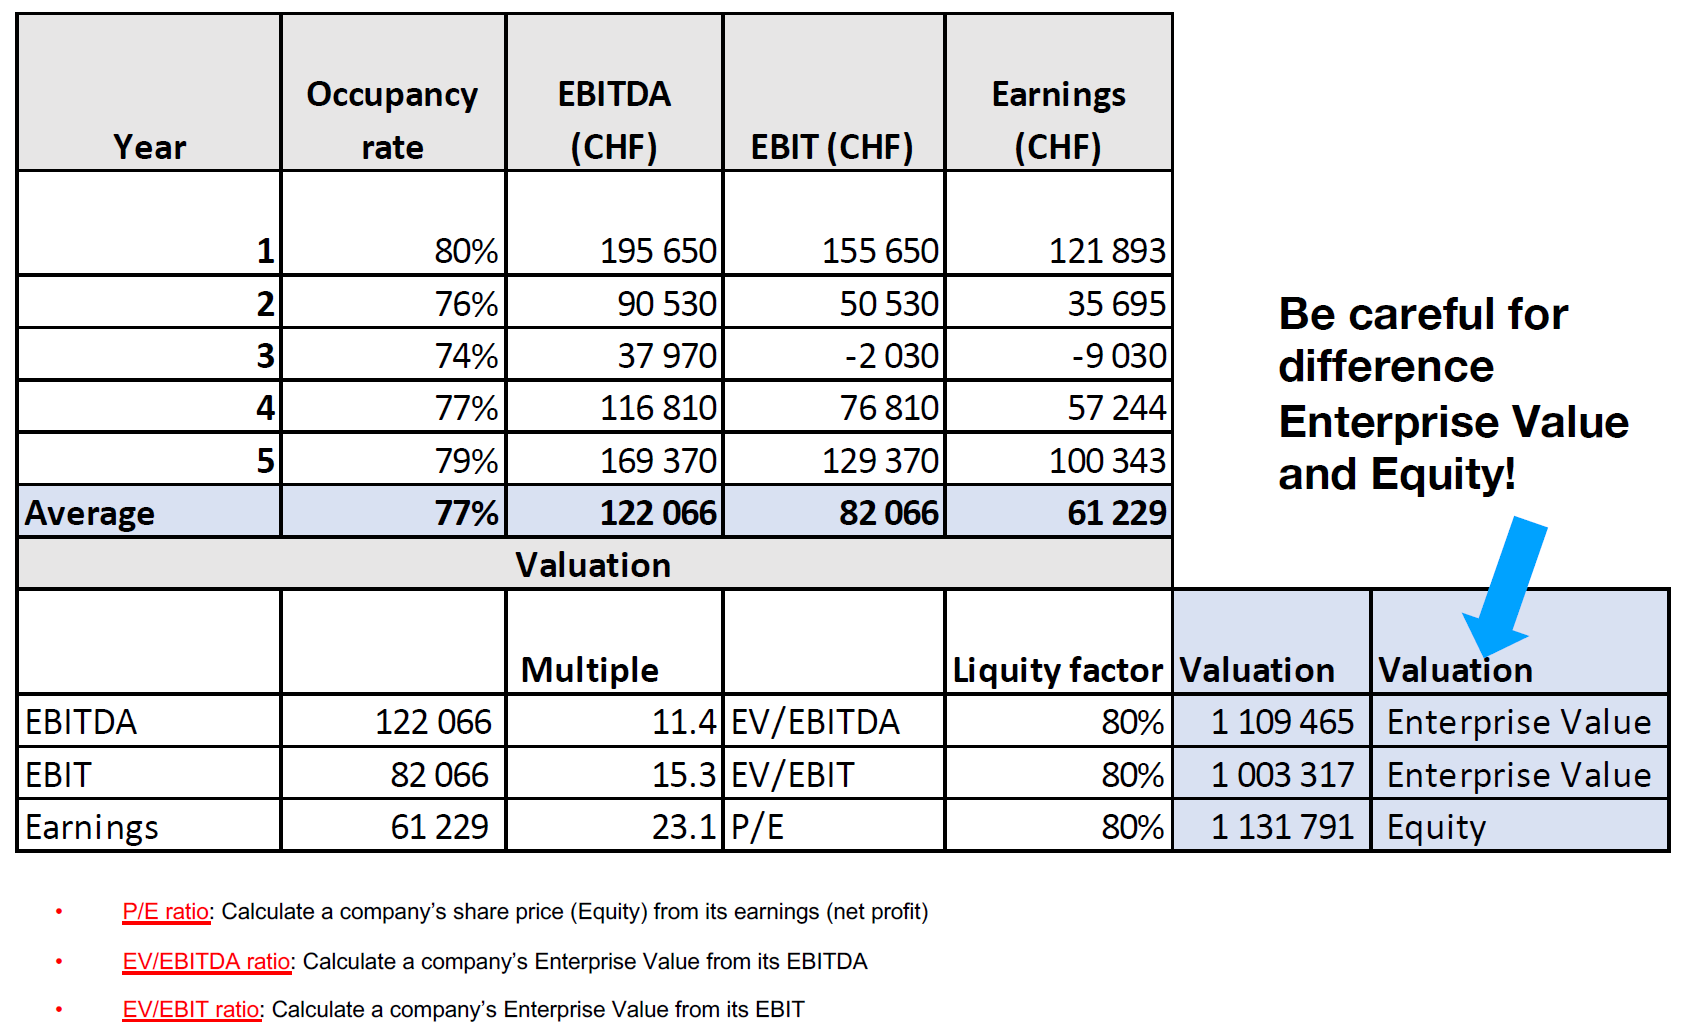
\includegraphics[width=0.7\textwidth]{Pictures/Valuation_taxi.png}
\end{figure}


\subsection{Cash-Flow Statement}
The Cash flow statement consists of three parts: operating activities, investing
activities and financing activities.
\begin{itemize}
    \item Operating Cash flow = Net income + Non cash expenses - increase in Working capital
        \begin{itemize}
            \item Change in Working capital: $\Delta$WC = change in accounts receivable + change in inventory - change in accounts payable
            \item There is a risk of growing too quickly. As a start up when you grow very fast,
                your working capital can also increase very quickly because you have to pay
                your vendors early because they do not trust you and otherwise they will not
                supply, you do not get paid by clients because they have strong negotiation power
                or you have to increase your inventory. As a consequence you can get in serious
                liquidity problems and even go bankrupt because you grow too fast!
        \end{itemize}
    \item Cash Flow from Investing Activities = Purchase/Sale of Long-Term Assets (Capex)
        + Purchase/Sale of other businesses (M\&A) + Purchase/Sale of marketable securities
\item Cash Flow from Financing Activities = Issue/Repurchase equity + Issue/Repurchase Debt
        + Dividend Payments and other Items
\end{itemize}

\begin{figure}[H]
    \centering
    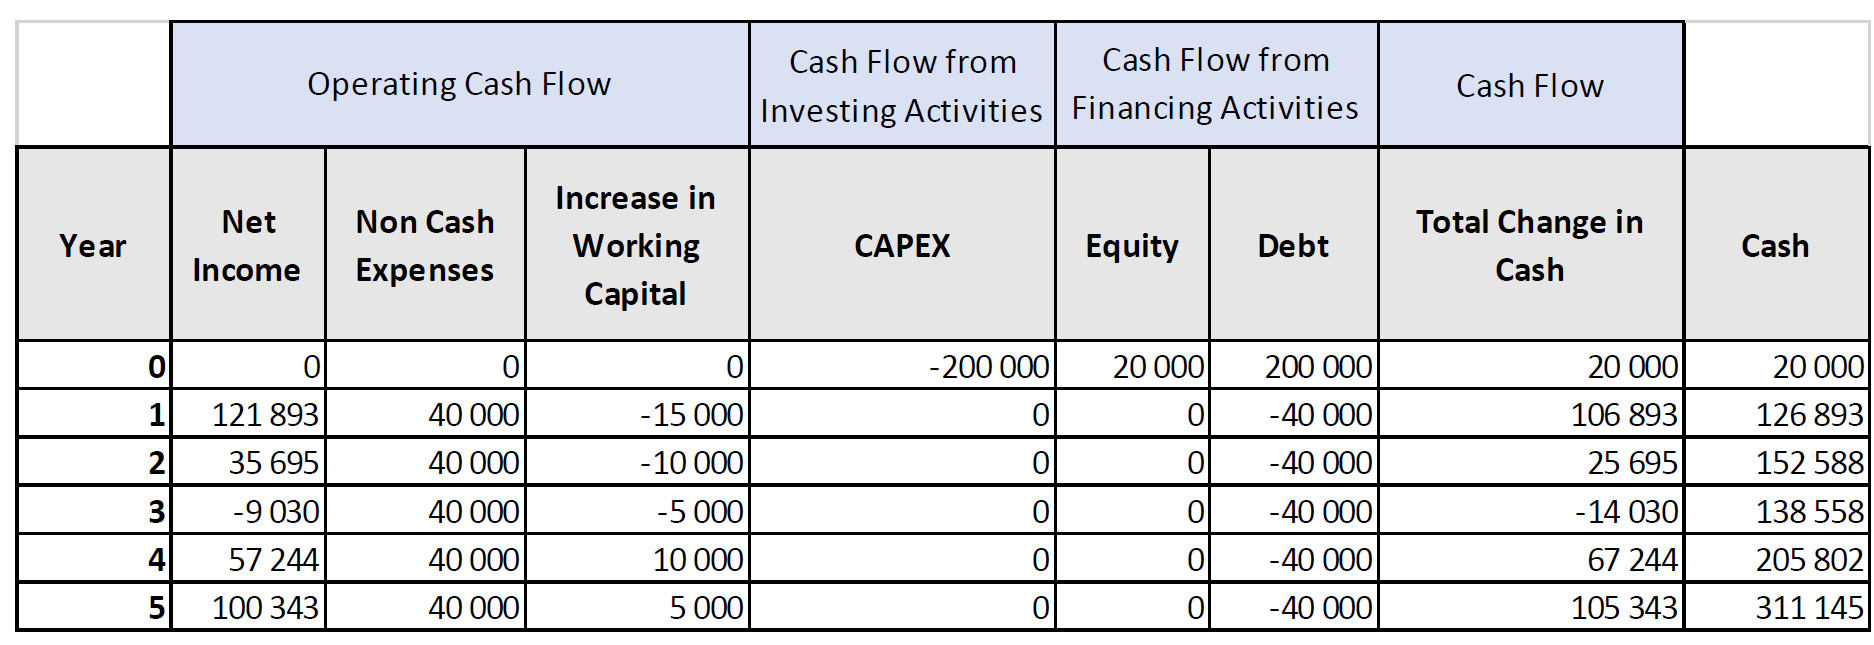
\includegraphics[width=0.8\textwidth]{Pictures/cash_flow_taxi_company.png}
    \caption{Cash flow from Taxi Business}
\end{figure}

\subsection{Company Valuation}

\paragraph{Time value of money}
The Formula for Future value:
\begin{align*}
    FV = PV \times (1+r)^n
\end{align*}
with $FV$ the future value, $PV$ the present value, $n$ the number of periods
and $r$ the rate of return or discount rate or interest rate or growth per period.

\paragraph{Price of a bond}
\begin{align*}
    \text{Bond Price} = \frac{C}{(1+i)} + \frac{C}{(1+i)^2} + \dotsb + \frac{C}{(1+i)^n} + \frac{M}{(1+i)^n}
\end{align*}
Where $C=$ coupon payment, $n=$ number of payments, $i=$ interest rate, or required
yield, $M=$ value at maturity, or par value.

\paragraph{Bonds vs. Stocks}
\begin{itemize}
    \item Bonds:
        \begin{itemize}
            \item Issues of debt
            \item Debt that is made with an investor for cash in exchange for payouts
                of interest.
            \item Typically traded over th ecounter (OTC)
            \item Generally lower risk, lower reward
            \item Since $1929$ have earned around $6\%$ each year
            \item Can be made as corporate, nunicipal, or treasury bonds
        \end{itemize}
    \item Stocks:
        \begin{itemize}
            \item Issues of a stake of ownership in a company
            \item A claim to a company's assets and earnings that often gives
                the investor voting rights and pays dividends
            \item Typically traded through a central exchange (like NYSE)
            \item Generally higher risk, higher reward
            \item Since 1929 have earned around $10\%$ each year
            \item Are issued by companies at a stock exchange as IPOs
        \end{itemize}
\end{itemize}

\paragraph{Discounted Cash Flow Valuation}
Present Value of Discounted Cash Flows:
\begin{align*}
    PV = \frac{CF_1}{(1+r)^1} + \frac{CF_2}{(1+r)^2} + \dotsb + \frac{CF_n}{(1+r)^n}
    = \sum_{i=1}^\infty \frac{CF_i}{(1+r)^i}
    = \sum_{i=1}^\infty \frac{CF_0 [1+g]^i}{(1+r)^i}
    = CF_0 r' \sum_{i=0}^\infty r'^i
    = CF_0 \frac{r'}{1 - r'}
\end{align*}
with $r' = \frac{1+g}{1+r}$, $CF$ the cash flow for a period, $r$ the discount rate and $n$ the number of
periods.
\begin{itemize}
    \item The value of a company can be calculated as the present value of a string
        of cash flows.
    \item There is no maturity so $n = \infty$
    \item Cash flows are not simple coupons like with a bond but must be estimated
    \item $r$ is not the yield of the bond, but is a discount rate that reflects the
        return that the investor expects unter the base case. It depends on the risk
        perception of the investor, higher risk will be high $r$ and vice versa.
\end{itemize}

Valuing a mature business with cash flow growing steadily at $g$:
\begin{align*}
    PV = CF_0 \frac{1+g}{r-g} = \frac{CF_1}{r-g}
    \hspace{10pt} \Rightarrow \hspace{10pt}
    \frac{PV}{CF_1} = \frac{1}{r-g}
    \hspace{10pt} \Rightarrow \hspace{10pt}
    r = \frac{CF_1}{PV} + g
\end{align*}
\begin{itemize}
    \item This is called the dividend discount model or the Gordon-Shapiro formula:
        total return is dividend yield + growth rate
    \item If the company is in a steady state of constant growth, the discounted
        cash flows formula can be written in the form of a multiple
\end{itemize}

\paragraph{Valuing a young company with a $5$ year start-up phase}
\begin{align*}
    PV = \sum_{i=1}^5 \frac{CF_i}{(1+r)^i} + \frac{TV}{(1+r)^5}
    = \sum_{i=1}^5 \frac{CF_i}{(1+r)^i} + \frac{\eckigeklammer{\frac{CF_6}{r' - g}}}{(1+r)^5}
\end{align*}
with $r$ the target rate of return during start-up phase and $r'$ the target
rate of return of mature business.
\begin{itemize}
    \item We discount the estimated cash flows during the start-up phase individually
    \item We calculate the TV (Terminal Value) of the company $5$ years in the future,
        when it has reached a state of maturity growth.
    \item We discount this TV
    \item This is like pricing a bond with estimated coupons and an estimated
        notional value
\end{itemize}

\paragraph{Discount rate}


\begin{itemize}
    \item Cashflows are discounted at a target rate of return, this is set high
        enough to capture business risk and the likelihood that the firm will
        not survive.
    \item Rates decrease as firms move through the life cycle and the chance of
        failure drops.
\end{itemize}

\begin{table}[H]
    \centering
    \begin{tabular}{|c|c|}
        \hline
        Stage of developmend & Typical target rates of return \\ \hline
        Start up & $50\% - 70\%$ \\ \hline
        First stage & $40\% - 60\%$ \\ \hline
        Second stage & $35\% - 50\%$ \\ \hline
        Bridge / IPO & $25\% - 35\%$ \\ \hline
    \end{tabular}
    \caption{Venture capital target rates of return - Stage in Life Cycle}
\end{table}

\begin{table}[H]
    \centering
    \begin{tabular}{|c|c|c|c|c|}
        \hline
        & $3$ years & $5$ years & $10$ years & $20$ years \\ \hline
        Early/Seed VC & $4.90 \%$ & $5.00\%$ & $32.90\%$ & $21.40\%$ \\ \hline
        Balanced VC & $10.80\%$ & $11.90\%$ & $14.40\%$ & $14.70\%$ \\ \hline
        Later Stage VC & $12.40\%$ & $11.10\%$ & $8.50\%$ & $14.50\%$ \\ \hline
        All VC & $8.50\%$ & $8.80\%$ & $16.60\%$ & $16.90\%$ \\ \hline
        NASDAQ & $3.60\%$ & $7.00\%$ & $1.90\%$ & $1.90\%$ \\ \hline
        S\&P & $2.40\%$ & $5.50\%$ & $1.20\%$ & $8.00\%$ \\ \hline
    \end{tabular}
    \caption{Returns earned by Venture Capitalists - 2007}
\end{table}

The actual annual returns earned by VCs at every stage of the process are much
more modest. The high target rates of return that are used for discounting are
not delivered because of the low survival rate.

\paragraph{Summary}
Three ways of valuation:
\begin{itemize}
    \item The balance sheet valuation gives you the company's book value,
        that is its shareholders' equity (capital and reserves), or the
        difference between its assets and liabilities.
    \item This does not take into consideration the fact that a company is
        'a little machine' or 'a process' that generates profit based on people
        (knowledge, learning,\dots), processes (strategy,organisation) and
        stuff (assets,technology,\dots)
    \item If you buy a company, you buy a little profit-making machine (or loss?).
        So it makes sense to use profit generation as a basis in the valuation.
        That is when you do relative valuation based on market calibrated
        multiples and different metrics in the P\&L, e.g. EBITDA, EBIT, net profit,\dots
    \item However, this supposes that the company is in a sort of 'steady state'
        or 'dynamic equilibrium'. For a growth company, earnings will
        increase in the future ans so will its valuation.
    \item For companies that are structured for growth, the discounted cash flow
        approach is needed (however, here a new parameter enters the equation,
        being the discount factor).
\end{itemize}

\subsection{Limits of markets,complex systems and financial bubbles}

\paragraph{Geometric Brownian Motion}
\begin{align*}
    \frac{dP}{P} = \mu \ dt + \sigma \ dW
\end{align*}
with $\frac{dP}{P}$ the percentage return over a time interval $dt$,
$\mu dt$ the drift over a time interval $dt$ and $\sigma dW$ the volatility
over a time interval $dt$. Stocks are supposed to have a constant drift, that
is the return part of the equation, accompanied by random shocks, that is the
risk part of the equaion. The geometric brownian motion random walk implies
that prices follow an exponential track decorated with noise. This is
equivalent to saying that growth rates are constant, that is why market
movements are mostly communicated as percentage changes and not as
dollar changes.

\paragraph{Bubbles}
\begin{itemize}
    \item A bubble starts with a new opportunity or expectation (e.g. a ground-braking
        technoloty)
    \item Smart money flows in, which leads to a first price appreciation
    \item Attracted by the prospect of higher returns, less sophisticated investors follow
    \item Demand goes up as the price increases, and the price goes up as the demand
        increases. This creates a positive feedback mechanism. The market is fully
        driven by behaviour and sentiment and no longer reflects any real
        underlying value.
\end{itemize}

\paragraph{Crash}
\begin{itemize}
    \item At some point, investors start realizing that the process is no
        longer sustainable and the market collapses.
    \item The crash occurs because the market has entered an unstable phase.
        Like a ruler held up vertically on your finger, any small disturbance
        could have triggered the fall.
    \item This mechanism is often not well understood, and a great controversy
        risis about the cause of the crash.
\end{itemize}

\paragraph{Exogenous vs. endogenous processes}
\begin{itemize}
    \item For exogenous processes cause and effect are linearly and logically
        connected. What is important is the trigger, e.g. for the impact of
        an asteroid, the state of the system is irrelevant.
    \item For endogenous processes cause and effect are not linearly connected.
        What is important is the state of the system. Any small event can
        trigger a major incident at some bifurcation points.
\end{itemize}

\paragraph{Complex Systems}
"Complex" does not simply mean "Complicated", is has a very specific meaning:
A complex System consists of a large ensemble of agents, like molecules,
stars, insects, mammals or even human beings. These interact, e.g. they may
repel, attract or imitate each other. Having a large set of interacting
agents is not enough. A system is said to be "complex", when there is
"Emergence", that is when local interactions lead to global cooperation,
in absence of any global orchestration. The whole is different that the sum
of its parts ("More is different" is a quote by Phil Anderson). "More is
different": one star does not make a galaxy; one molecule cannot freeze.
Local interactions lead to global structures.

\paragraph{Emergence}
Coordination in absence of orchestration. Local interactions lead to global
cooperation and self-organization.

\paragraph{Dynamics of human systems}
By imitation and internal organization groups of people may exhibit a global
coorporation. Emergence appears and the mass behaves like a complex system
similarly to a swarm, this is endogenous, there is no master of ceremony at work.
Under such circumstances it is often quite deceptive to follow a cause-and-consequence
reason, what is most important is the state of the system. Any small event can
trigger a major incident.


\pagebreak

\section{Wrapping up the deal}

Before we draft the legal documents, we need to agree on the most important
principles of the deal:
\begin{itemize}
    \item The amount invested, and how it will be made available (in one single
        payment, or in tranches dependent on milestones)
    \item The value of the company (with a distinction between pre- and post money
        valuation)
    \item The cap table, who owns what percentage of the company
    \item The Governance principles
\end{itemize}

\subsection{The amount invested}

In the example of Company $X$, we decided to invest $2$M Euro's. This was
our base case scenario. The investment amount turned out to be too small
and follow up rounds were needed. Investors may have an incentive to start
with a low initial investment, if things go well they will have a higher
ROI, if things go bad, they can invest the additional amount at a lower
company valuation. As a founder/entrepreneur, it is important to negotiate
for a strong cash buffer. If the cash burn is higher than expected, you may
need to find new capital in a situation under stress. At that time your
company valuation will be lower and you will dilute (start losing ownership
of the company).

\subsection{Value of the Company}

\begin{figure}[H]
    \centering
    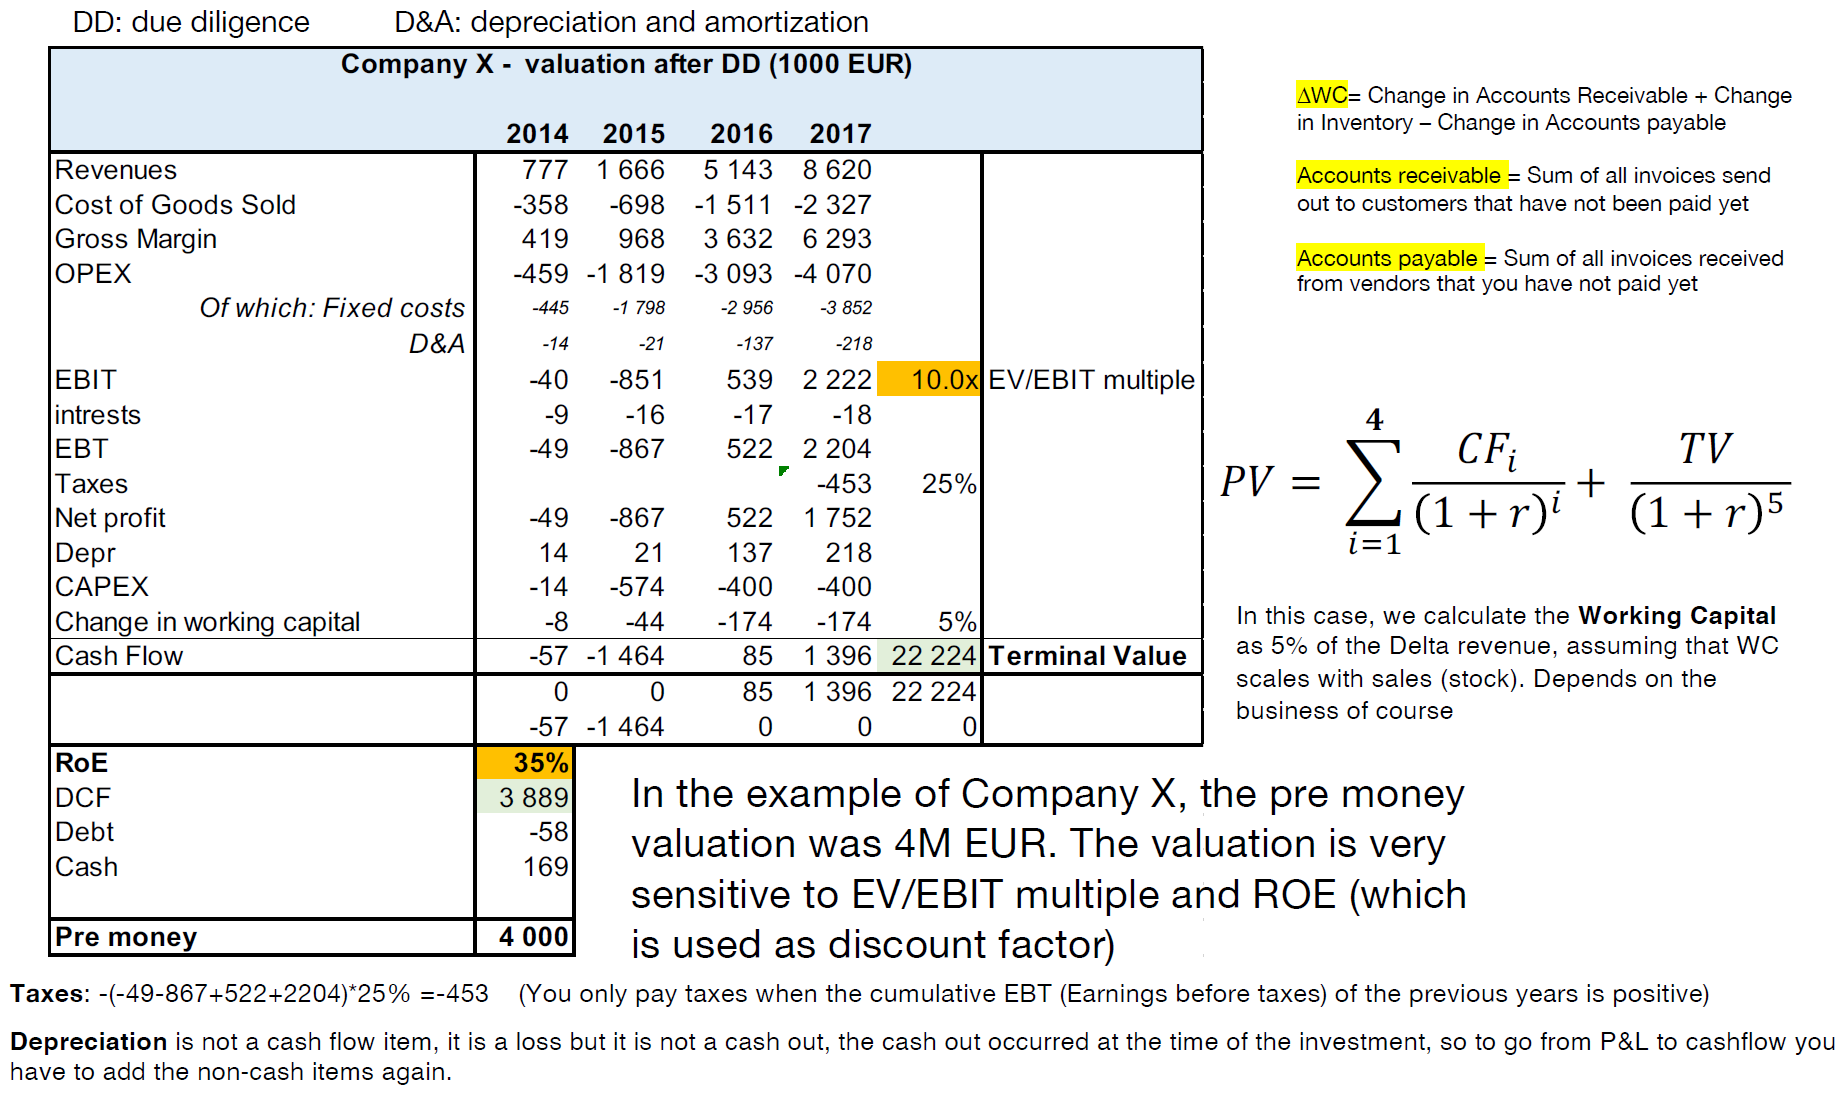
\includegraphics[width=0.9\textwidth]{Pictures/value_of_the_company.png}
    \caption{Value of the Company}
\end{figure}

\begin{figure}[H]
    \centering
    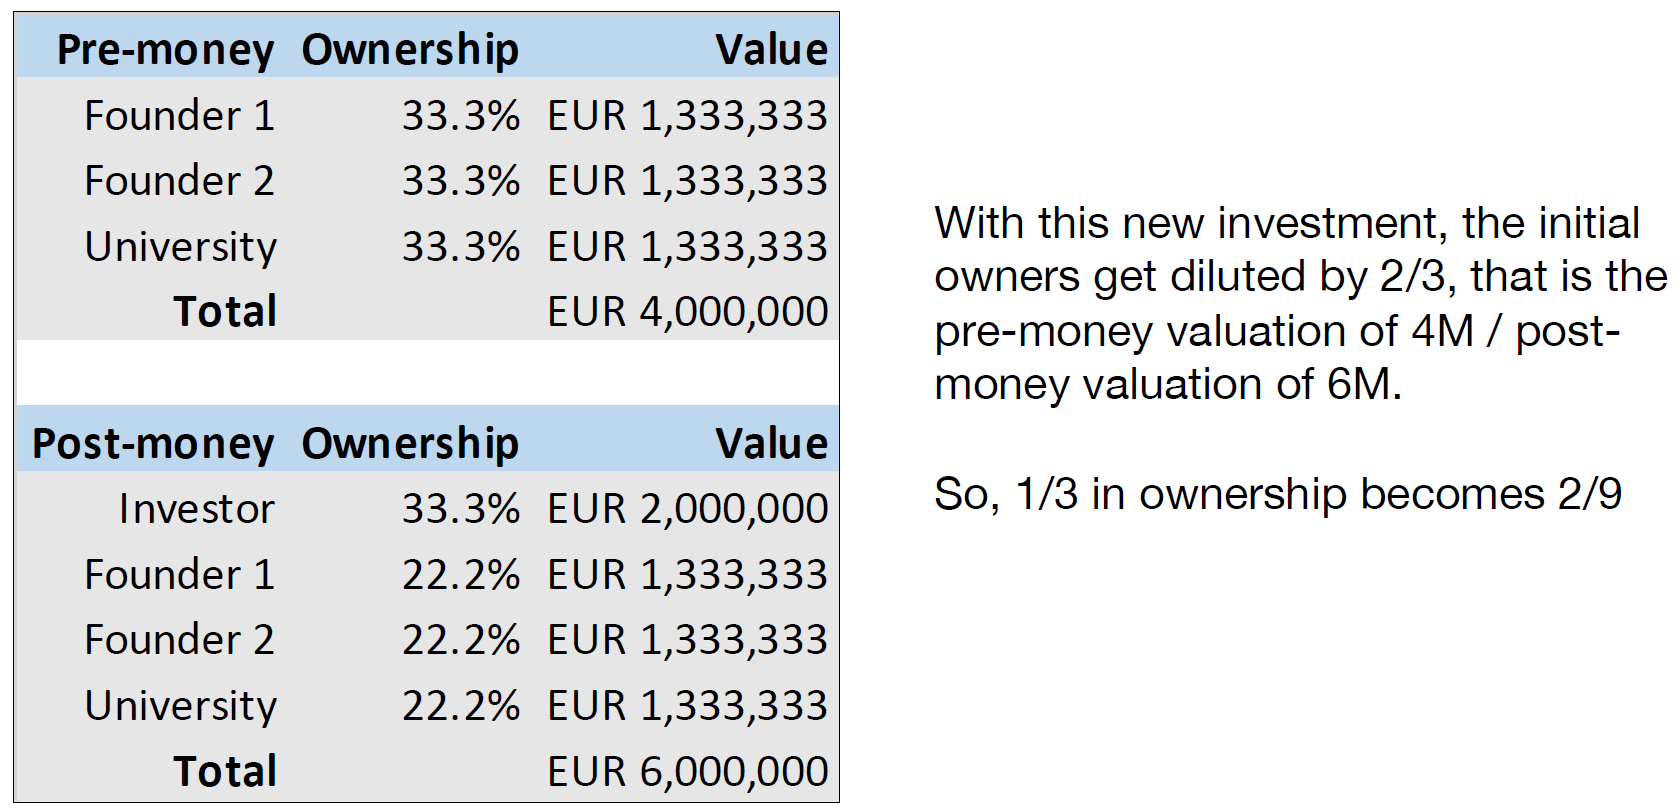
\includegraphics[width=0.6\textwidth]{Pictures/pre_and_post_money.png}
    \caption{Pre- and Post money}
\end{figure}

\subsection{Cap Table}

Capitalization Table: Specifying ownerships, equity value, etc.

\subsubsection{Governance principles}

\begin{enumerate}[]
    \item \underline{What?}: To outline the responsibility, the composition and the
        authority (the decisions making process) of the Management Team (MT), the
        Supervisory Board (SVB) and the General Meeting of Shareholders (GMS) of
        the company.
    \item \underline{Why?}: To allow for an efficient management of the company
        based on objective criteria and processes independently of existing persons
        and historical relationships.
    \item \underline{How?}: By writing or changing the article of association and/or
        the shareholder agreement, where needed.
\end{enumerate}

\subsubsection{Corporate Bodies}

Consists of three parts: General Meeting of Shareholders, Supervisory Board,
Management Team.

\paragraph{Management Team} Day-to-Day affairs

\begin{itemize}
    \item Directs the company's day-to-day affairs
    \item Has the authority to decide in line with the annual budget and business
        plan that has been approved by the board.
    \item In case of significant deviation from the budget and the business plan,
        the decision is escalated to the board.
    \item Often a matrix is drafted showing clearly the decision authority
        of each or multiple MT members ordered according to subject, amount,
        signing authority \dots
\end{itemize}

\paragraph{Supervisory Board} Supervision

\begin{itemize}
    \item Composed of representatives of the shareholders + independent board
        members (non-executive) + senior management (executive)
    \item Composition and voting rights are clearly defined in the shareholders
        agreement.
    \item Must supervise and advise the management and oversee the general affairs
        within the company.
    \item Should be guided by the interests of the company.
\end{itemize}

\paragraph{Supervisory Board, Typical decision authority of the board}

\begin{itemize}
    \item Hire/fire of senior management
    \item Adoption and/or amendment of yearly business plan and budget
    \item Investment, loans, contracts \dots exceeding a threshold
    \item Option plan for employees
    \item Targets and variable remuneration of senior management
\end{itemize}

\paragraph{General meeting of Shareholders} Value creation

\begin{itemize}
    \item Composed of the shareholders (owners) of the company
    \item May give priority to their own interests with due regard for the
        principles of reasonableness and fairness
    \item Meets at least once per year to approve the annual accounts,
        discharge the board and follow up and/or adapt the Value Creation
        Plan (long term business plan)
    \item Appoints the members of the Supervisory Board and sometimes also
        members of the management team (like the CEO)
    \item Decides by majority unless explicity stated differently in the
        shareholder agreement.
\end{itemize}

\paragraph{General meeting of Shareholders, Typical decision authority
of shareholders:}

\begin{itemize}
    \item issue of new shares
    \item hire/fire new CEO
    \item distribution of dividends
    \item Reorganisation of the business
    \item Application for bankruptcy
    \item Debt restructuring
    \item Acquisition of another company
    \item Sale to - or merger with another company
    \item \dots
\end{itemize}

\subsubsection{Legal Documents}

Once the amount invested, the value of the company, the cap table, and the
governance principles are agreed upon, the legal documents are drafted.
The main documents are the following:
\begin{itemize}
    \item Subscription Agreement (the transaction)
    \item Shareholders Agreement (governance and organisation)
    \item Management Agreement (day-to-day operations)
\end{itemize}
When everything goes fine, these documents will never be read again after signing
at the notary office. But remember that they are written for when things go wrong
e.g. in business, but also in private life or health\dots

So one important part of the legal documents is to prescribe how a 'divorce'
between different parties can be arranged!

\paragraph{Subscription Agreement}

\begin{itemize}
    \item A Subscription Agreement is between a company and private investor to
        sell a specific number of shares at a specific price.
    \item It contains, amongst others, information regarding the amount
        invested, the cap table, issues of new shares or transfer of
        existing shares, payment conditions, conclusions on the due diligence,
        warranties,\dots
    \item Some agreements include a specified rate of return that investors
        are guaranteed to receive (the so-called 'preference shares')
\end{itemize}

\paragraph{Shareholders Agreement} Governance and organisation

\begin{itemize}
    \item A shareholders' agreement describes how the company should be operated
        and outlines shareholders' rights and obligations.
    \item Is intended to make sure that all shareholders are treated fairly
        and that their rights are protected.
    \item Outlines the governance principles: the responsibility, the
        composition and the authority of the Management Team (MT), the
        Supervisory Board (SVB) and the General Meeting of Shareholders
        (GMS) of the company.
    \item Describes the exit scenario (transfer of shares) with specific care
        for the rights of minority as well as majority shareholders.
\end{itemize}

\paragraph{EXIT / Transfer of shares}


\begin{enumerate}[]
    \item \underline{Lock-up}: A predetermined amount of time where shareholders
        are restricted from selling their shares.
    \item \underline{Right of first refusal}: After the lock-up period, when
        one shareholder can sell shares to a third party, the other shareholders
        must be given the opportunity to match the price and buy shares instead
        of the third party.
    \item \underline{Drag along (protection of majority shareholder)}:
        \begin{itemize}
            \item A drag along right allows a majority shareholder of a company
                to force the remaining minority shareholders to accept an offer
                from a third party to purchase the whole company at the same price,
                terms and conditions.
            \item Drag-along rights help eliminate minority owners and sell $100 \%$
                of a company's securities to a potential buyer.
        \end{itemize}
    \item \underline{Tag along (protection of minority shareholders)}
        \begin{itemize}
            \item Tag along rights are inverse of drag along rights. When a majority
                shareholder sells their shares, a tag along right will entitle the
                minority shareholder to participate in the sale at the same time for
                the same price.
            \item The minority shareholder then 'tags along' with the majority
                shareholder's sale.
        \end{itemize}
\end{enumerate}

\paragraph{Good leaver / Bad leaver}

A description of the circumstances in which a person ceases to be an employee
of a company $\rightarrow$ For founders, often this leads to forced selling of
the shares.

\begin{enumerate}[]
    \item \underline{Good leave}: usually due to serious illness, disability to
        work, death or (early) retirement $\rightarrow$ Founders get 'market
        value' for their shares.
    \item \underline{Bad leave}: voluntary leave before end of contract,
        compelling cause (e.g. criminal activity,\dots) $\rightarrow$ Founders
        get way less than 'market value' for their shares.
\end{enumerate}

\paragraph{Management Agreement} (day-to-day operations)

Agreement between the management and the company outlining.
\begin{itemize}
    \item Exchange management services
    \item Management fee
    \item Variable remuneration (bonus)
    \item Targets and objectives
    \item Duration and termination of the contract
    \item Intellectual property rights
    \item Non-competiiton
    \item Condidentiality
\end{itemize}

\subsubsection{Negotiation}

Finalisation of the legal documents may take quite some time. There will be
negotiations and small print will be read and discussed in great detail.

\subsubsection{Signing at the notary office}

The final step is to sign the contract at the notary office.



\pagebreak

\section{The logistic equation of growth, saturation and diffusion}

\subsection{The logistic equation}

Growth and saturation in an environment with competition for limited resources.
The size of a population, with competition for limited resources, grows according to
a very specific process. It has an $S$-shape.

\subsubsection{Mathematical formulation}

Logistic differential equation:
\begin{align*}
    \frac{dP}{dt} = r P(t) \eckigeklammer{1 - \frac{P(t)}{K}}
\end{align*}
In the beginning ($P(t) << K$), for small $t$, we have exponential growth.
Later $P(t)$ plateaus and reaches the constant value of $K$.

\subsubsection{Mathematical solution}

With $P_0$ the initial population ($P(t=0)=P_0$). The solution, called
logistic function, is:
\begin{align*}
    P(t) = \frac{K P_0 e^{r t}}{K + P_0 (e^{r t} - 1)}
\end{align*}

\subsubsection{Different representations of logistic growth}

\begin{figure}[h]
    \centering
    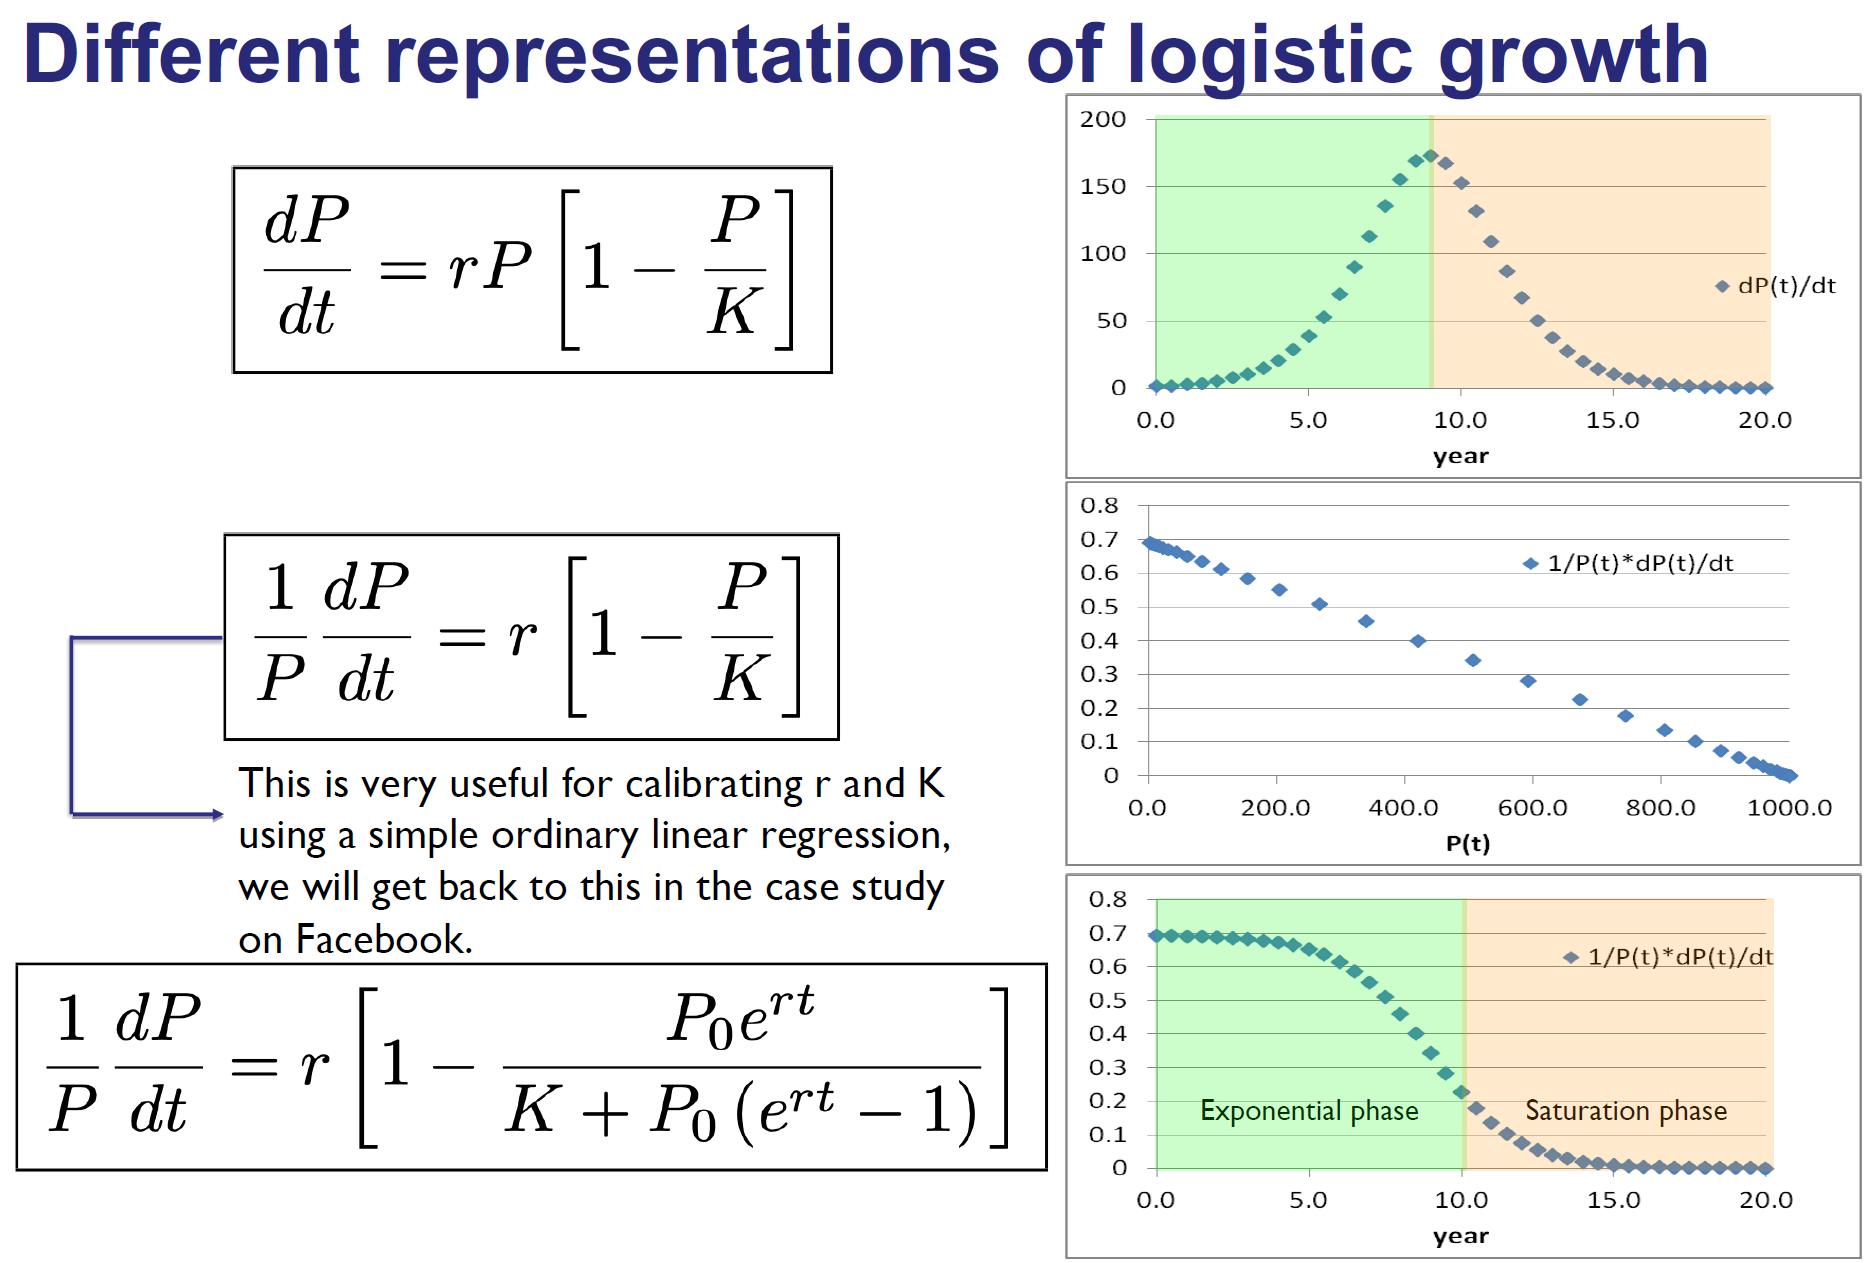
\includegraphics[width=0.6\textwidth]{Pictures/log_growth_diff_rep.png}
\end{figure}

\subsubsection{The Hubbert model and peak oil}

Oil production rates, in Gb/Year (billion barrels per year) were modelled using
the following equation:
\begin{align*}
    \frac{dP}{dt} = \frac{A}{1 + \cosh \eckigeklammer{-B (t-C)}}
    \hspace{10pt} \Rightarrow \hspace{10pt}
    P(t) = \frac{2 A}{B} \frac{1}{1+e^{-B(t-C)}}
\end{align*}
This is equivalent to the logistic equation, or that we referred to as the Varhulst
Growth Model, with
\begin{align*}
    K = \frac{2A}{B}
    \hspace{10pt} , \hspace{10pt}
    r = B
    \hspace{10pt} , \hspace{10pt}
    P_0 = \frac{K}{1 + e^{BC}}
\end{align*}

\subsubsection{Two types of models to describe epidemics}

\paragraph{Phenomenological models}

An empirical approach without a specific basis on the physical laws or mechanisms
that give rise to the observed patterns in the data. Emphasize the reproducibility
of empirical observations using simple models.

\paragraph{Mechanistic models}

Incorporate key physical laws or mechanisms involved in the dynamics of the
problem under study (e.g. population or transmission dynamics) in order
to explain patterns in the observed data. Often formulated in terms of a dynamical
system describing the spatial temporal evolution of a set of variables and are useful
to evaluate the emergent behaviour of the system across the relevant space of parameters.

\subsubsection{Population growth - Exponential}

\begin{itemize}
    \item Population increases in proportion to their size
    \item E.g. at a $10 \%$ annual rate if increase
        \begin{itemize}
            \item a population of 100 adds 10 individuals in one year
            \item a population of 1000 adds 100 individuals in one year
        \end{itemize}
    \item Allowed to grow unchecked, populations growing at a constant
        rate will rapidly approach infinity.
    \item This is known as exponential growth $C_t = C_0 e^{r t}$ where $C_t$
        is the population size, $r$ is the instantaneous (per capita) rate of
        increase and $t$ is time.
\end{itemize}

\subsubsection{Generalized growth model}

We can relax the assumption of exponential growth via "scaling of growth"
perameter $p$:
\begin{align*}
    \frac{dC}{dt} = r C^p (t)
\end{align*}
where $\frac{dC}{dt}$ describes the incidence growth phase over time $t$, the
solution $C(t)$ describes the cumulative number of cases at $t$.
\begin{itemize}
    \item $p=0$: this equation describes constant incidence over time and
        cumulative number of cases grows linearly.
    \item $p=1$: well-known exponential growth model.
    \item $0<p<1$: sub-exponential (e.g. polynomial) growth patterns.
    \item $1<p$: super exponential growth leading to finite-time singularity.
\end{itemize}

\subsubsection{Extension of Logistic type model}

\begin{itemize}
    \item Generalized-logistic growth model (GLM):
        \begin{align*}
            \frac{dC}{dt} = r C^p \klammer{1 - \frac{C}{K}}
        \end{align*}
    \item Richards model:
        \begin{align*}
            \frac{dC}{dt} = r C \klammer{1 - \klammer{\frac{C}{K}}^\alpha}
        \end{align*}
    \item Generalized Richards model (GRM):
        \begin{align*}
            \frac{dC}{dt} r C^p \klammer{1 - \klammer{\frac{C}{K}}^\alpha}
        \end{align*}
    \item The two additional parameters introduced:
        \begin{itemize}
            \item Parameter $p \in [0,1]$, describes the "scaling of growth"
                as in the generalized growth model and allows for sub-exponential
                growth during the early stage of the growth.
            \item Parameter $\alpha \geq 0$ measures the extent of deviation from the
                S-shaped dynamics of classical logistic growth model. Controls
                asymmetry.
        \end{itemize}
\end{itemize}

\pagebreak

\subsection{Generalized logistic growth modeling of the Covid-19 outbreak}

Plots can be seen in the Lecture slides of Lecture $5$.

\begin{figure}[h]
    \centering
    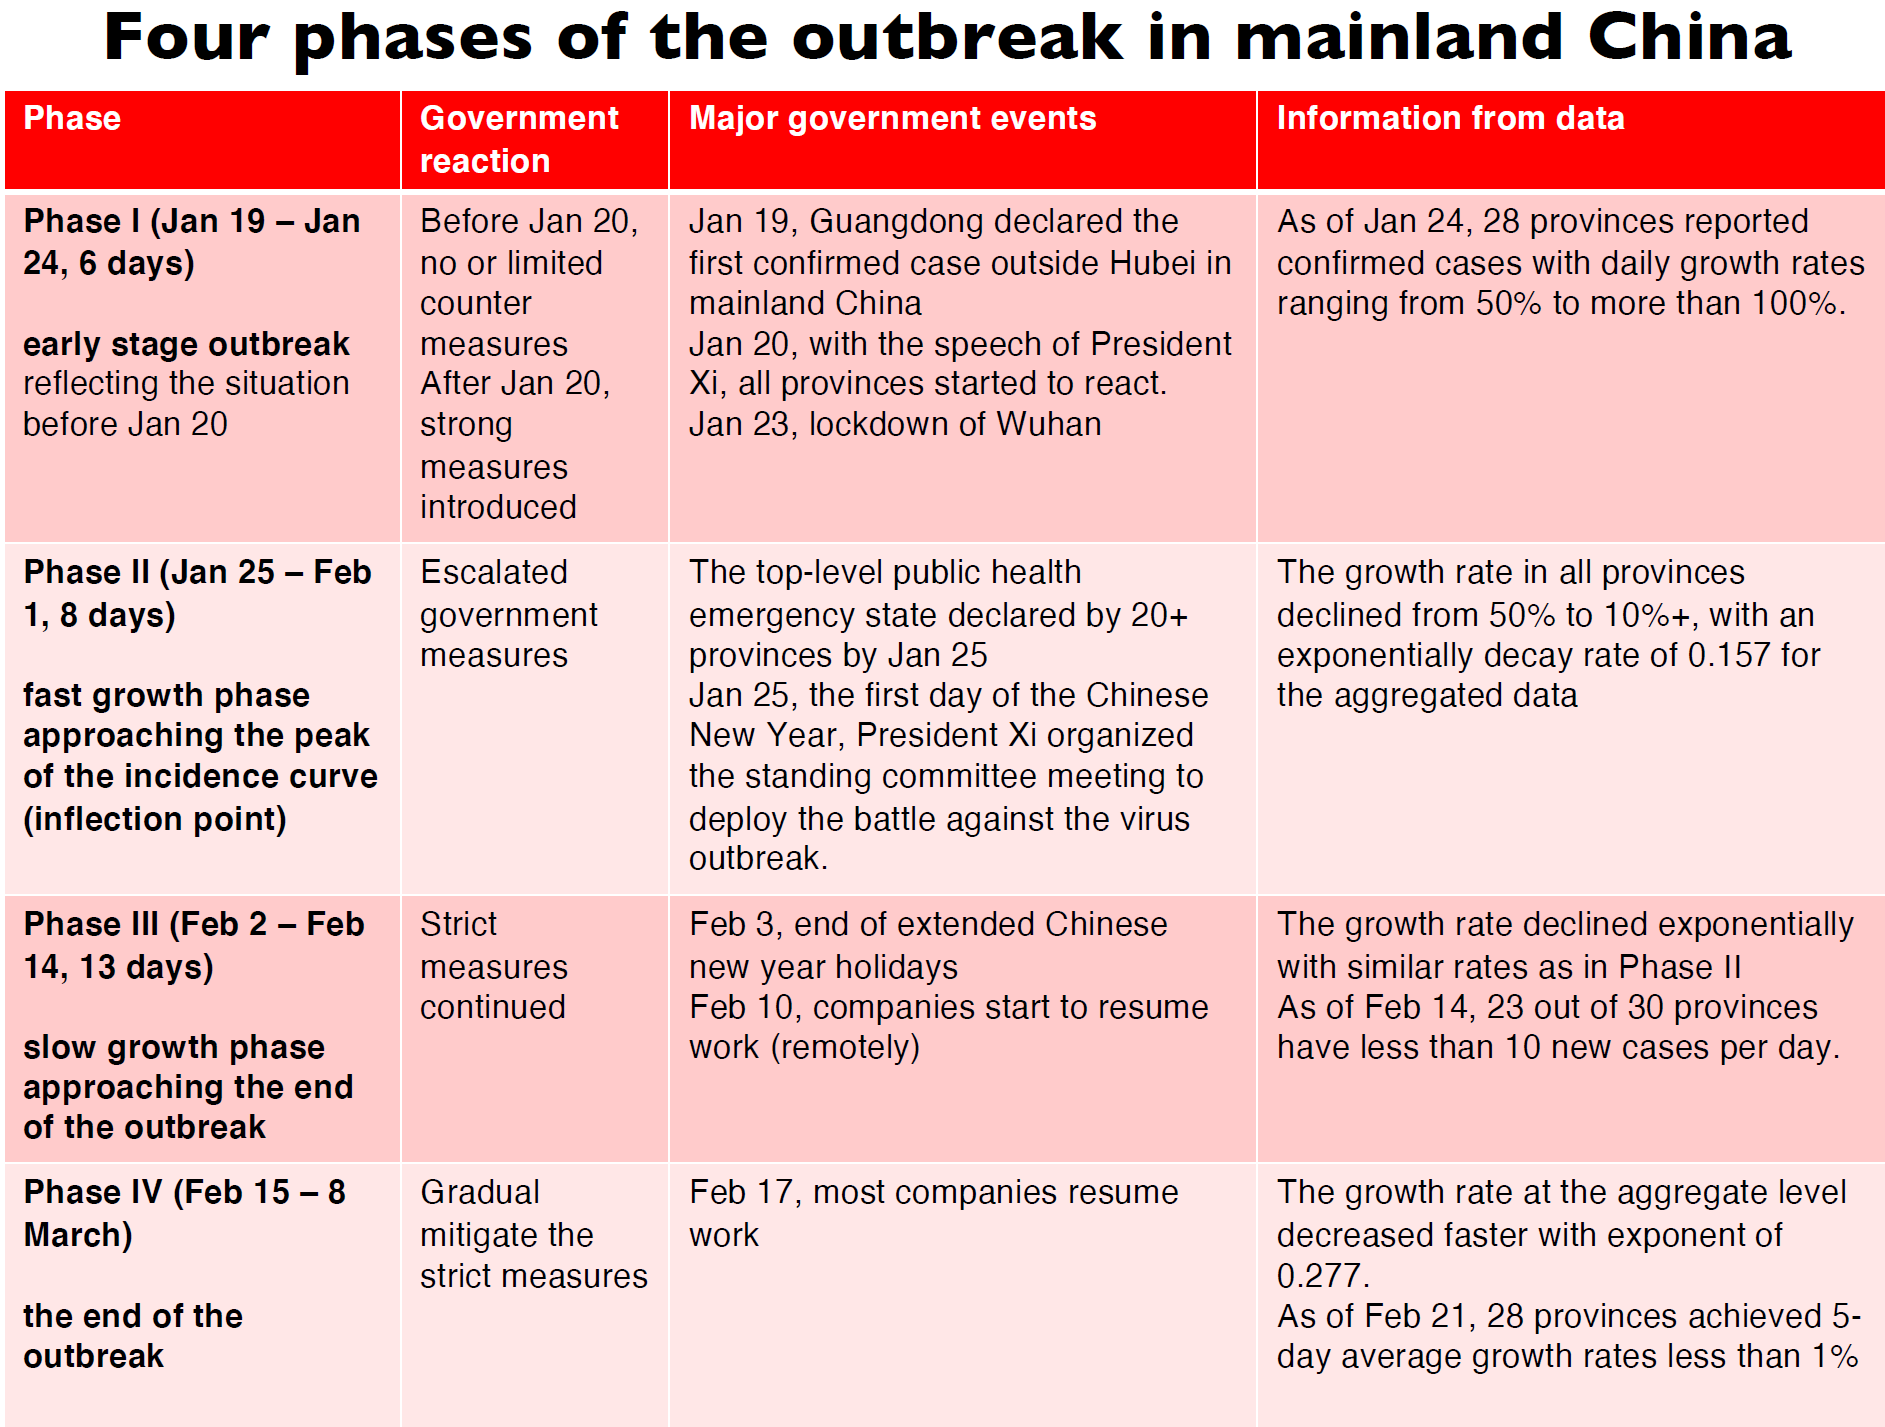
\includegraphics[width=0.9\textwidth]{Pictures/four_phases_of_the_outbreak_in_mainland_china.png}
\end{figure}

\begin{itemize}
    \item For countries in the early or middle stage of the outbreak, GRM is too
        flexible. Thus we consider the three simpler models with fewer parameters:
        the classical Logistic growing model, the Generalized-logistic growth model
        (GLM), and the generalized growth model.
    \item The classical Logistic growing model and Generalized-logistic growth
        model (GLM) tend to underestimate the number of infected cases, and the
        generalized growth model tend to overestimate the number of cases, which
        nicely serve as positive and negative scenarios for the future developments.
\end{itemize}

\paragraph{South Korea approach}

\begin{itemize}
    \item Korea doesn't have a tech solution, they have a solution that uses tech.
        It's different. When it comes to contact tracing, Korea didn't reinvent the
        wheel. They just used technology to dramatically speed it up. The Korean
        system allowed them to trace contacts in as little as $10$ minutes, which
        is unheard of. It's like everyone else is on bicycles and Korea has a bullet
        train.
    \item Everyone's talking about apps. Get everyone to install an app and, boom,
        contact tracing. That's not how it works. Korea did not rely on an app for
        contact tracing. Instead of an app, they used a wide constellation of data
        a board, redundant set of data combed over by trained people.
    \item One key insight is speed. All of their technology, all of their
        bureaucracy is just there to make their response as fast and agressive
        as possible. That's the only way to beat an exponential disease.
\end{itemize}


\paragraph{Summary}

\begin{itemize}
    \item Ultimately, the Covid-19 pandemic is a low-level stressor (anyone can
        imagine much worse stressors) BUT the consequences will be severe and
        disproportionate due to the mismanagement and unbalanced monodimensional
        responses.
    \item The guiding principle of our time: CYA (cover your ass) (active
        throughout time but now in "hyper-drive") Hyper-judicialization
        (appearing to save lives now is what counts)
    \item CYA explains the response of governments, Italy following China, and
        the rest of Europe (except Sweden) following Italy.
    \item In a society that aims at the mirage of "zero risk", lack of courage
        to follow a course of action and management based on scientific knowledge.
    \item Developing real-time research to inform decisions is like trying to
        develop GPS in the time of the sextant. Research takes time.
    \item $\Rightarrow$ considerable increase of uncertainties catalyzed by normal
        conflicts between scientists.
    \item This amounts to a devastating failure of leadership and courage.
\end{itemize}


\subsection{Generalization of logistic equations}

\begin{enumerate}[]
    \item \underline{Observation}: many systems exhibit succession of $S$-curves
        because advances in technology etc. increase the carrying capacity $K$.
    \item \underline{Idea}: include this into the logistic equation with a
        population dependent carrying capacity with delay time $\tau$.
        \begin{align*}
            \frac{d P}{d t} &= r P(t) \eckigeklammer{1 - \frac{P(t)}{K(t)}}
            \hspace{15pt} \text{with} \hspace{15pt}
            K(t) = A + B P(t - \tau)
            \\
            \Rightarrow
            \frac{d x}{d t} &= x(t) - \frac{x^2(t)}{a + b x(t - \tau)}
        \end{align*}
        with $x \sim P$ and parameters $a,b$ related to $r,A$ and $B$.
\end{enumerate}

\subsubsection{Generalized logistic growth equation}
\begin{align*}
    \frac{d x}{d t} = \underbrace{x(t)}_{\text{individual growth/gain term}}
        - \underbrace{\frac{x^2(t)}{a + b x(t-\tau)}}_{\text{competition term}}
\end{align*}
\underline{Solution}: the solution space is extremely rich and can be categorised
according to $a$ and $b$. Four possible scenarios:
\begin{align*}
    \frac{d x}{d t} &= x(t) - \frac{x^2(t)}{a + b x(t-\tau)}
    \hspace{20pt} \text{(gain and competition)}
    \\
    \frac{d x}{d t} &= x(t) + \frac{x^2(t)}{a + b x(t-\tau)}
    \hspace{20pt} \text{(gain and cooperation)}
    \\
    \frac{d x}{d t} &= - x(t) - \frac{x^2(t)}{a + b x(t-\tau)}
    \hspace{20pt} \text{(loss and competition)}
    \\
    \frac{d x}{d t} &= - x(t) + \frac{x^2(t)}{a + b x(t-\tau)}
    \hspace{20pt} \text{(loss and cooperation)}
\end{align*}

\subsubsection{Nonlinear carrying capacity}

\begin{enumerate}[]
    \item \underline{Idea}: instead of a linearly growing carrying capacity,
        consider the case of exponential growth:
        \begin{align*}
            \frac{d x}{d t} &= \sigma_1 x(t) - \sigma_2 \frac{x^2}{y(x)}
            \hspace{15pt} \text{with} \hspace{15pt}
            y(x) = \exp \klammer{b x(t - \tau)}
            \\
            \Rightarrow
            \frac{d x}{d t} &= \sigma_1 x(t) - \sigma_2 x^2(t) e^{-b x(t - \tau)}
        \end{align*}
    \item We can distinguish $4$ cases:
        \begin{align*}
            \sigma_1 = 1 &, \sigma_2 = 1
            \hspace{20pt} \text{gain and competition}
            \\
            \sigma_1 = -1 &, \sigma_2 = -1
            \hspace{20pt} \text{loss and cooperation}
            \\
            \sigma_1 = -1 &, \sigma_2 = 1
            \hspace{20pt} \text{loss and competition}
            \\
            \sigma_1 = 1 &, \sigma_2 = -1
            \hspace{20pt} \text{gain and cooperation}
        \end{align*}
\end{enumerate}


\subsubsection{Coupled logistic equations}

\begin{enumerate}[]
    \item \underline{Idea}: instead of only one species, we can also have
        two interacting species $x$ and $z$.
        \begin{align*}
            \frac{d x}{d t} = x - \frac{x^2}{1 + b x z}
            \hspace{20pt} , \hspace{20pt}
            \frac{d z}{d t} = z - \frac{z^2}{1 + g x z}
        \end{align*}
\end{enumerate}

\subsection{Introduction to Chaos Theory}

\subsubsection{The logistic map}

The logistic map is defined by
\begin{align*}
    x(n+1) = \alpha x(n) \eckigeklammer{1 - x(n)}
\end{align*}
It can be shown that $x$ is chaotic for (almost all) values
$\alpha \in [3.569\dots,4]$.
It can be shown that the logistic map is nothing but a discretised version
of the logistic equation with $\alpha = r+1$.

\begin{figure}[H]
    \centering
    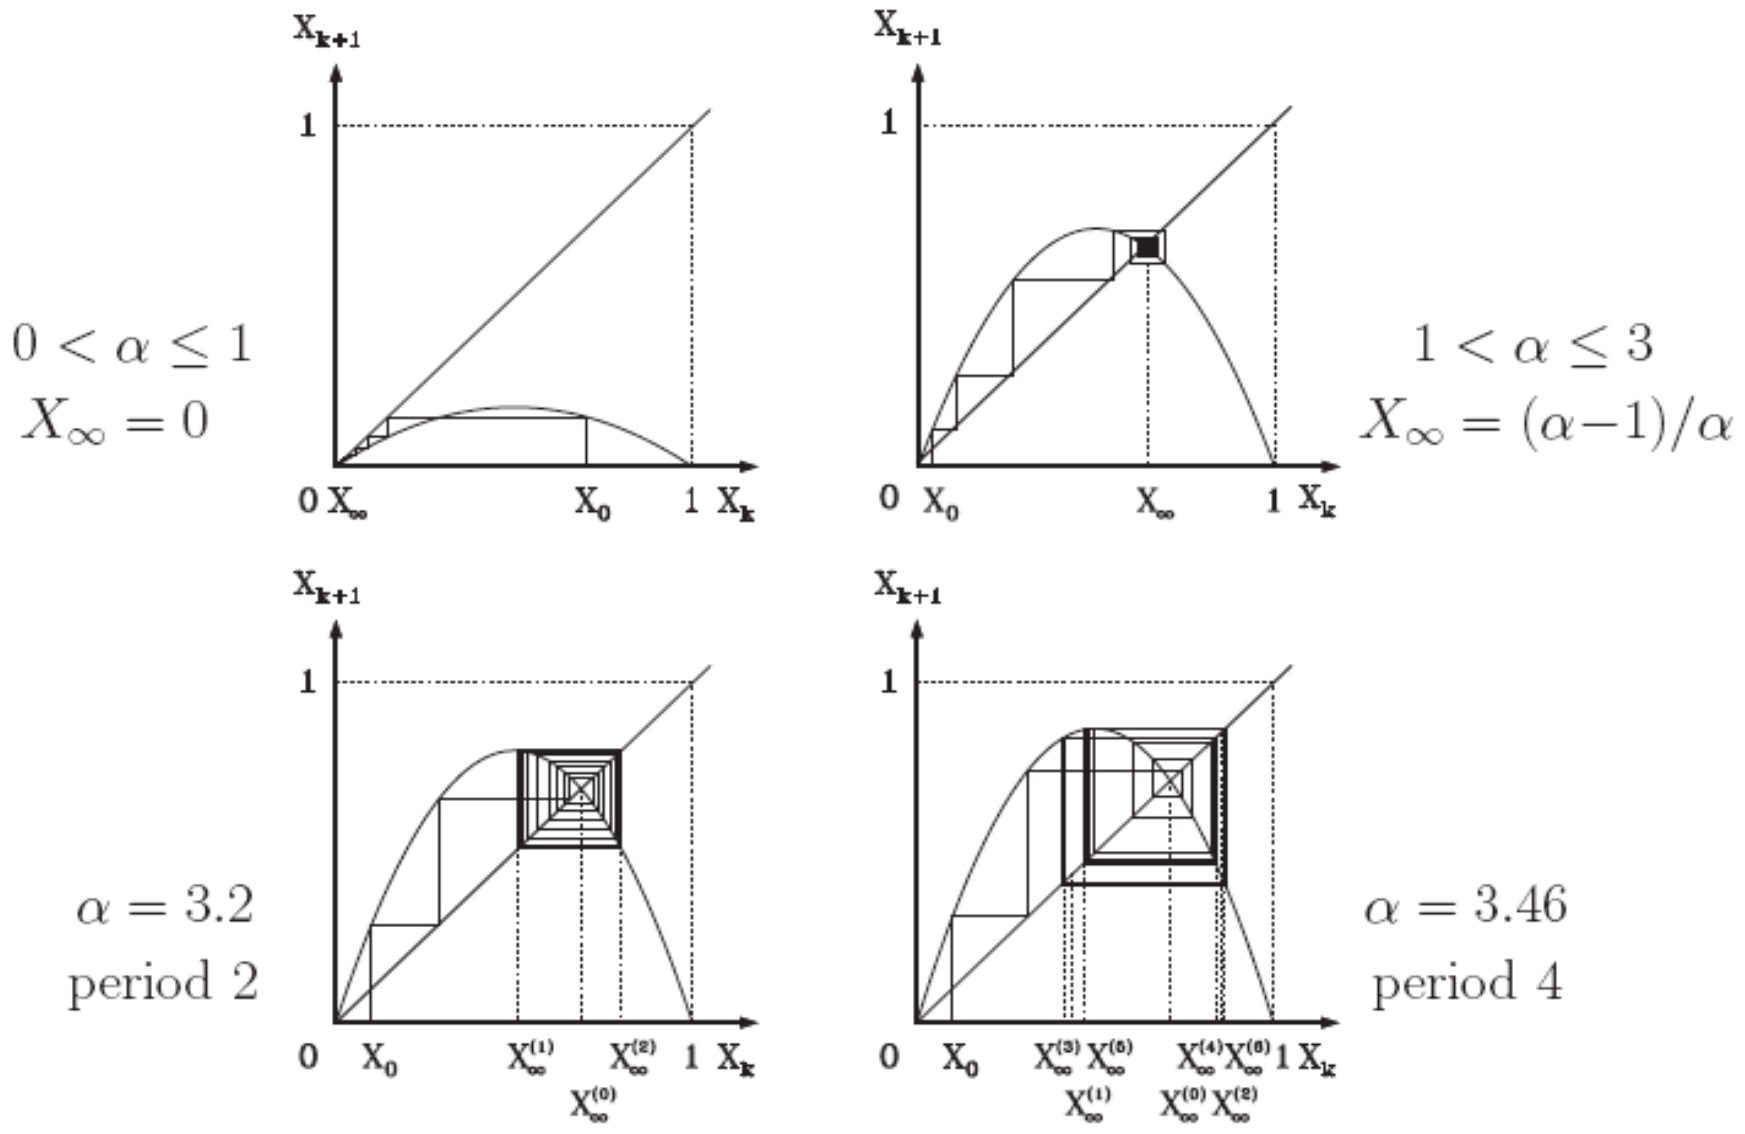
\includegraphics[width=0.7\textwidth]{Pictures/chaos_theory_intuition.png}
\end{figure}

\begin{figure}[H]
    \centering
    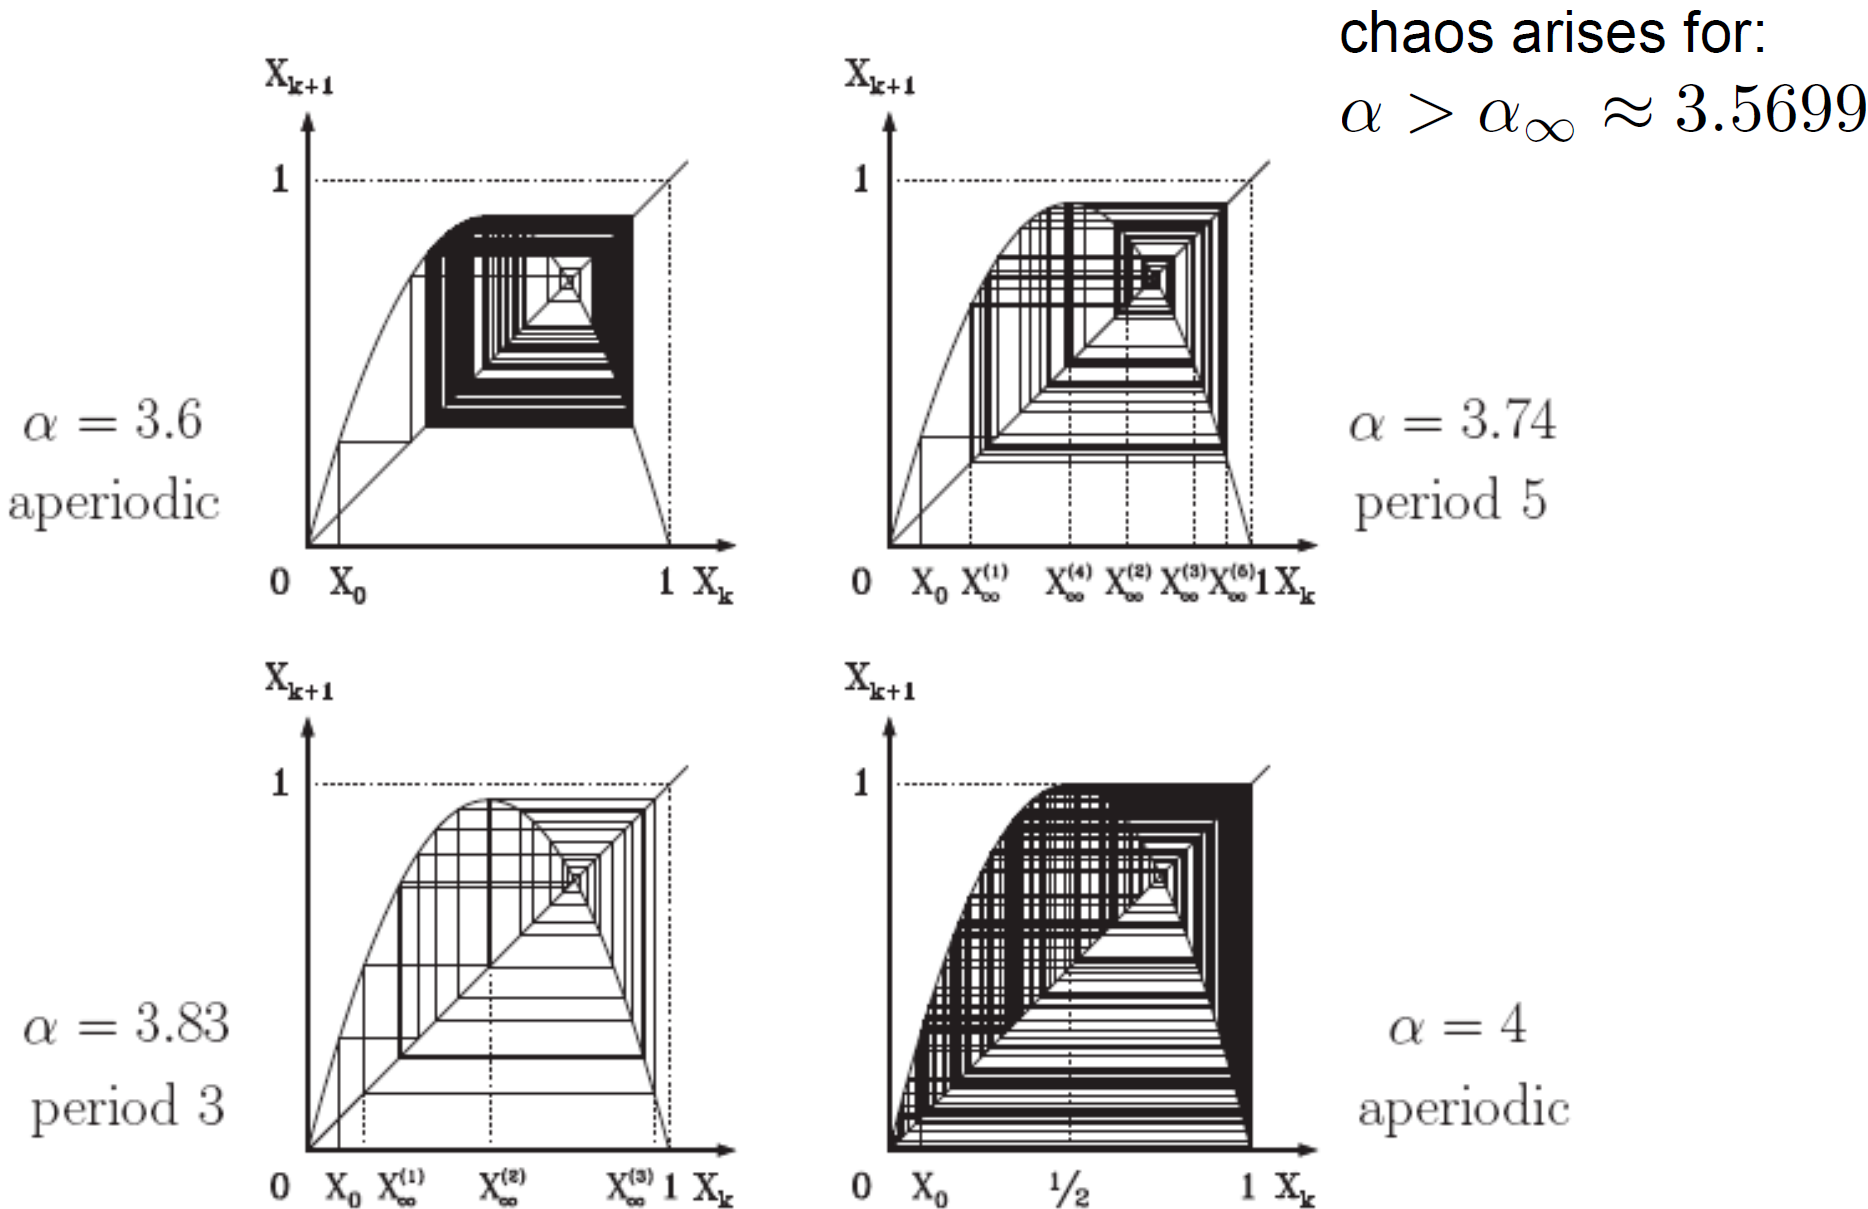
\includegraphics[width=0.7\textwidth]{Pictures/chaos_theory_intuition_2.png}
\end{figure}

\pagebreak

\paragraph{Bifurcation diagram}

\begin{figure}[H]
    \centering
    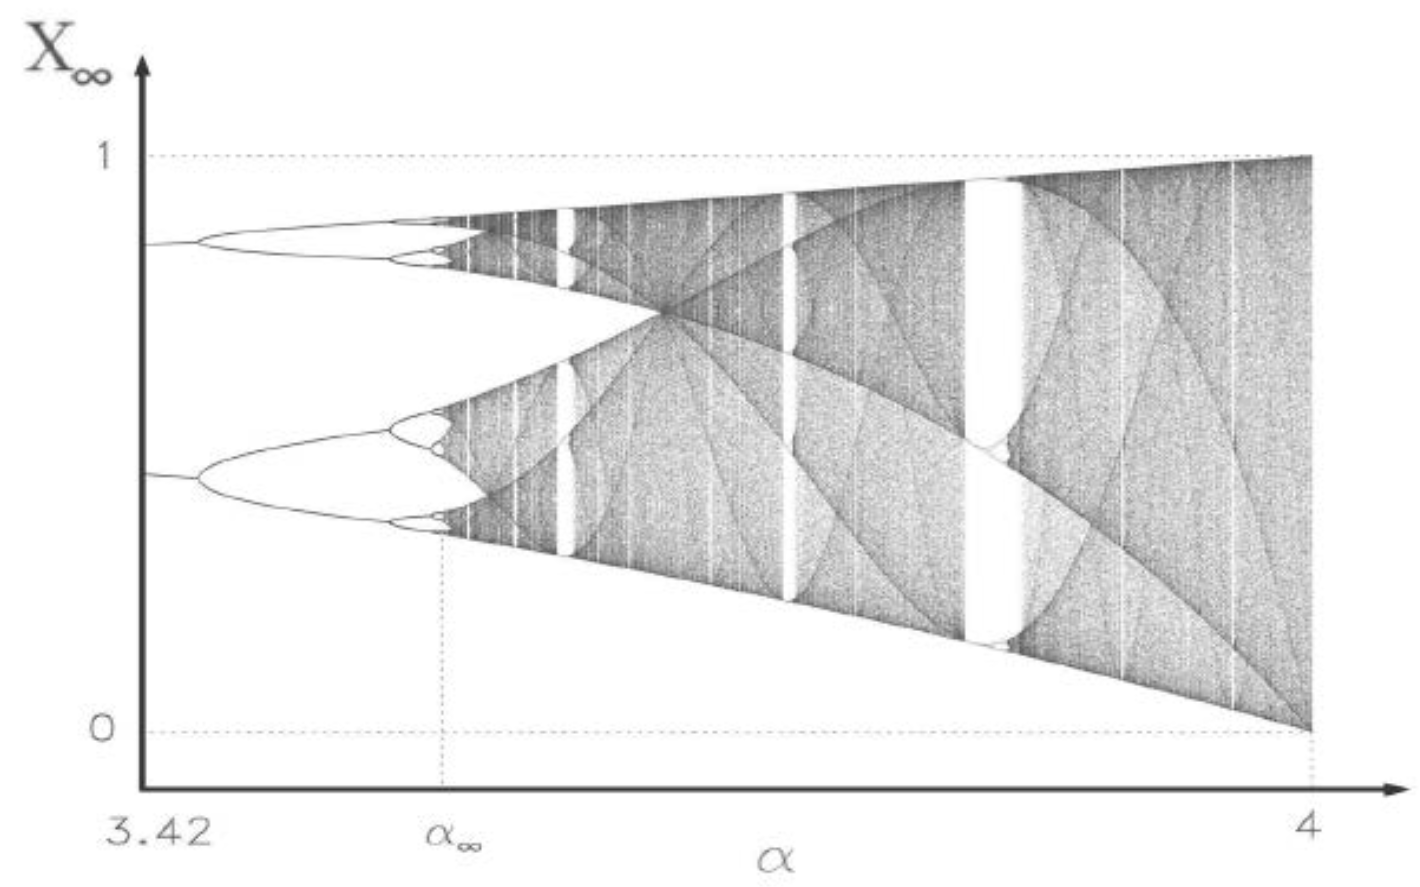
\includegraphics[width=0.7\textwidth]{Pictures/logistic_map_bifurcation_diagram.png}
    \caption{Bifurcation diagram}
\end{figure}

After $\alpha_\infty$, dusty "strange attractors" are common expansion of periodic
buds gives small copies of tree!


\subsubsection{Number Theory: roots of randomness}

It can be shown that the logistic map is equivalent to the tent map
\begin{align*}
    y(n+1) = 2y(n) \ \mod{1}
\end{align*}
with $x_n = \sin^2(2 \pi y_n)$ and $\alpha = 4$.
This explains the origin of the chaotic behaviour as fundamentally
embedded the mathematical properties of the digits of irrational numbers,
which are of measure $1$ among real numbers.

\subsubsection{Chaos}

\paragraph{Definition}
Chaos is not random, but due to a deterministic map $x: A \rightarrow B$
satisfying the following properties:
\begin{enumerate}
    \item $x$ is low dimensional
        \begin{itemize}
            \item $x$ is only dependent on a "small" number of variables,
                for instance: $x(n+1) = f(x(n),x(n-1),x(n-2))$. Nevertheless,
                the outcome is very complex!
        \end{itemize}
    \item $x$ is deterministic
        \begin{itemize}
            \item This means, that the next value can always be predicted exactly.
        \end{itemize}
    \item $x$ is sensitive to initial values
        \begin{itemize}
            \item Slight changes in the initial value can dramatically change
                the output.
        \end{itemize}
    \item trajectories of $x$ are reinjected
        \begin{itemize}
            \item Although slight differences in initial values $x1$ and $x2$
                lead to trajectories which can be arbitrarily far apart from
                each other, there will be a point at which these two trajectories
                are again arbitrarily close to each other.
        \end{itemize}
\end{enumerate}

\pagebreak

\subsection{The diffusion of innovation}

Focus questions: How does a new technology spread? How are new products
adopted by people in society?

\paragraph{Categories of adoption}

There are five different categories:

\begin{figure}[h]
    \centering
    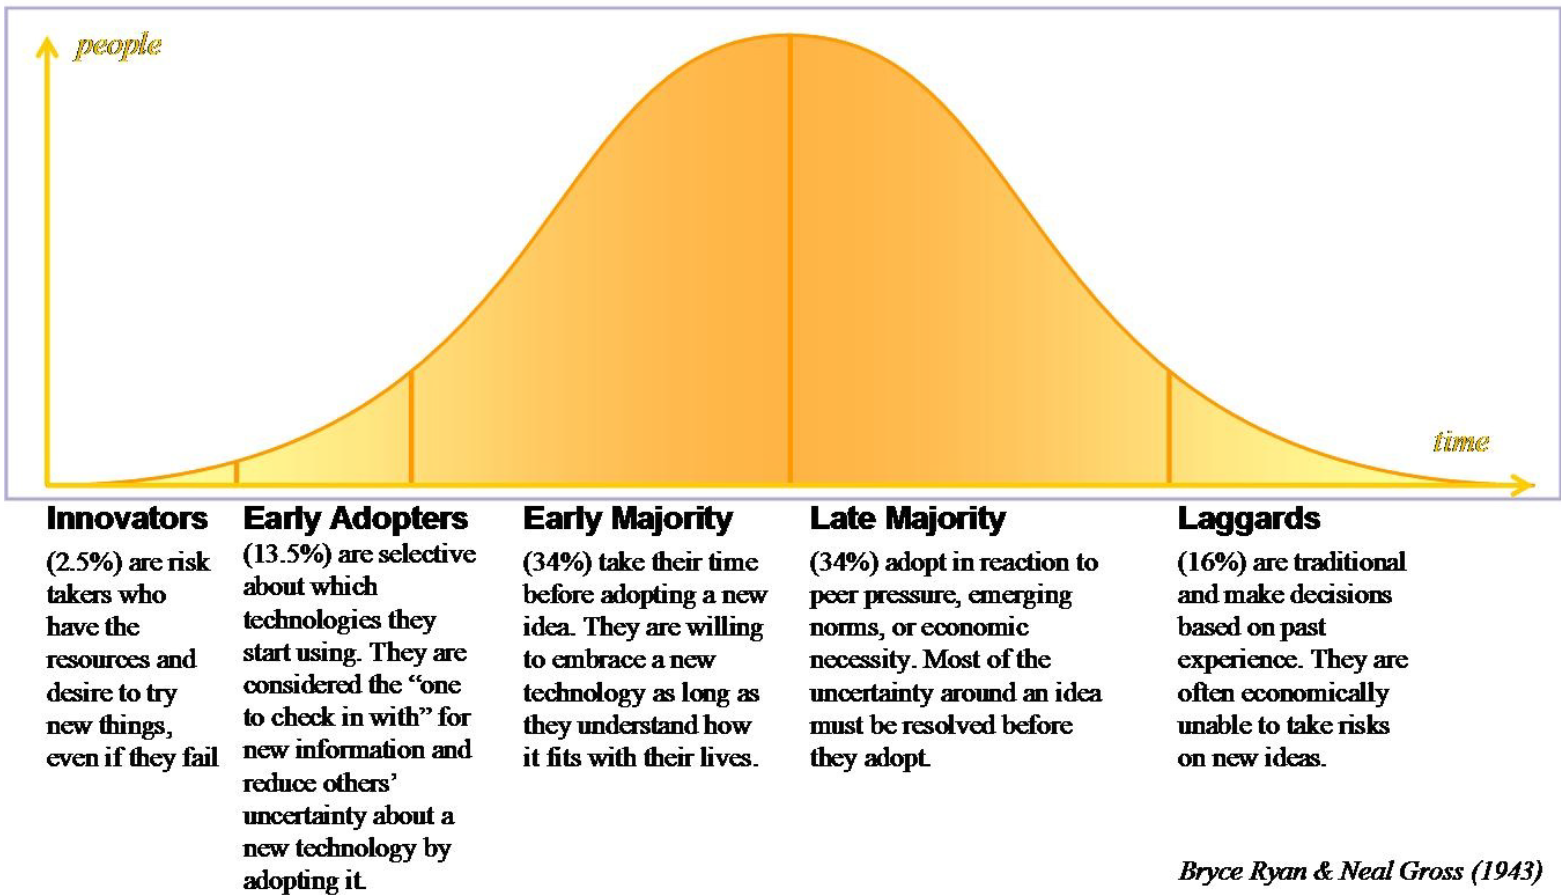
\includegraphics[width=0.7\textwidth]{Pictures/Categories_of_adoption.png}
\end{figure}

\paragraph{Terminology}

\begin{enumerate}[]
    \item \underline{Penetration rate}: The penetration rate is like the
        population size in Part \uproman{1}, it follows an S-shaped curve
        and saturates at 100\% when the full population has adopted the new
        technology.
    \item \underline{Penetration speed}: The penetration speed is comparable
        to the production rate, it follows a Gaussian shaped curve.
\end{enumerate}

\subsubsection{The Agent Based Model (ABM) of Namatame}

\paragraph{Definitions}

\begin{itemize}
    \item $F(t)$ is the \underline{penetration rate}, it is the fraction
        of the population that has adopted the new technology, this will
        follow an S-shaped curve, it is cumulative.
    \item $F(t+1) - F(t)$ is the penetration speed, it is the fraction
        of the population that adopts the new technology in the following
        time-step, this will follow a Gaussian-shaped curve.
    \item $p(t+1)$ gives the probability that an agent will adopt the new
        technology in the next time-step.
\end{itemize}

\begin{figure}[h]
    \centering
    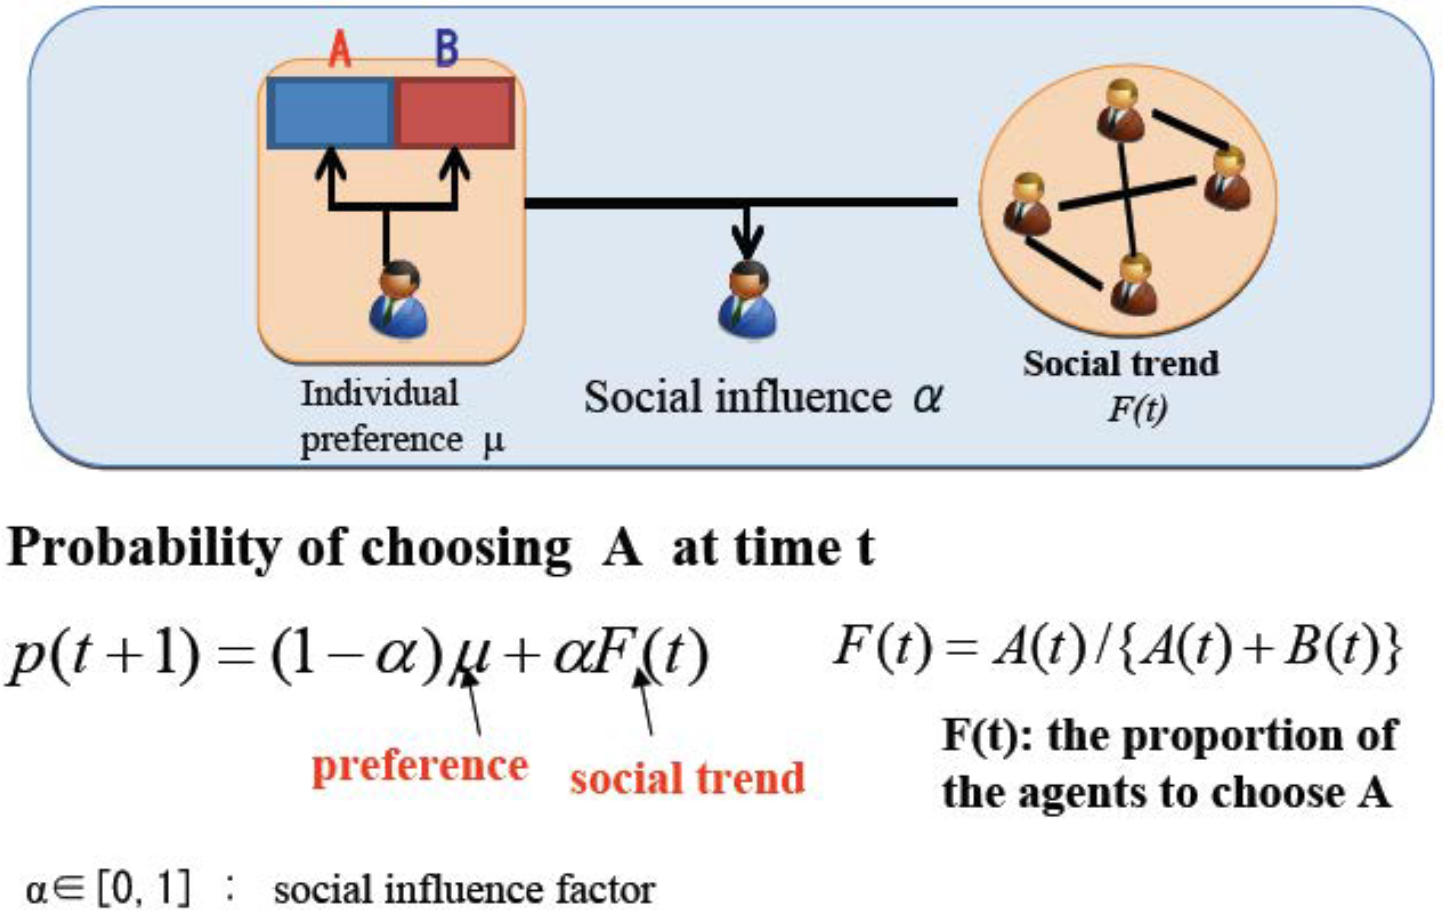
\includegraphics[width=0.55\textwidth]{Pictures/ABM_1.png}
\end{figure}

\paragraph{The Model}

\begin{itemize}
    \item $p(t+1) = (1 - \alpha) \mu + \alpha F(t)$. The first term corresponds
        to personal preferences (is a constant) and the second term corresponds
        to the social trend (A fraction of the penetration rate, the social
        trend increases as more people adapt).
    \item $p(t+1)$ only applies to agents that have not yet adopted, this
        concerns the fraction $(1-F(t))$ of the agents.
    \item As a consequence: $F(t+1) - F(t) = p(t+1) \cdot (1-F(t))$.
        The penetration rate is the probability that an agent adapts times
        the number of non-adapted agents.
    \item $F(t+1) = F(t) + p(t+1) \cdot (1-F(t)) = F(t) +
        \klammer{(1-\alpha) \cdot \mu + \alpha \cdot F(t)} \cdot (1-F(t))$
    \item In case there is no personal preference and only social interaction:
        \begin{itemize}
            \item $\mu = 0$
            \item $F(t+1) = F(t) + \alpha \cdot F(t) \cdot (1 - F(t))$
            \item In continuous form:
            \begin{itemize}
                \item $\frac{dF(t)}{dt} = \alpha \cdot F(t) \cdot (1 - F(t))$
                \item This is the logistic differential equation with $K=1$
                \item 100\% penetration rate agrees with a carrying capacity of 1
                \item $r = \alpha$
            \end{itemize}
        \end{itemize}
    \item In the case there is only personal preference, and no social
        interaction or context:
        \begin{itemize}
            \item $\alpha = 0$
            \item $F(t+1) = F(t) + \mu \cdot (1 - F(t))$
            \item continuous form:
            \begin{itemize}
                \item $\frac{dF(t)}{dt} = \mu \cdot (1 - F(t))$
                \item $F(t) = 1 - \exp(-\mu \cdot t)$
            \end{itemize}
            \item This is like radioactive decay, the concentration of
                the parent nuclei drops exponentially and the concentration
                of the doughter nuclei increases with $1 - \exp$. Indeed
                there is no interaction between the nuclei in radioactive
                decay.
        \end{itemize}
    \item The penetration rate differs for different levels of social
        interaction and varies between a process without any social
        interaction, like nuclear decay, and a process with a very strong
        social interaction, like the growth of rabbits.
\end{itemize}

\paragraph{Example: Diffusion of innovation}

Penetration rate as a function of time, more like a step function means more
social interaction, or more trendy products. If the diffusion speed is
parabolic, there is social interaction and if it is linear, there is no
social interaction.

\subsection{Case Study - the valuation of the company Facebook before the IPO}

Analysis: see Lecture slides of Lecture 6 on 14/04/2021.
\footnote{\url{https://xyotta.com/cfiles/1186}}

\paragraph{Greenshoe option}
\begin{itemize}
    \item A greenshoe option is also called an over-allotment option:
    \item At the IPO, the underwriters sold 15\% more shares then what was
        initially targeted, creating a big short position (2.4 billion USD)
    \item If the price goes up, covering this short would be extremely expensive
    \item When the underwriters execute the greenshoe option, Facebook must
        emit 15\% more shares at the IPO price. This allows them to cover their
        position without any loss.
    \item If the price goes below the IPO price, they can close the short
        position, buy back the shares at the IPO price and as such support
        the price at the IPO level.
\end{itemize}

Putting aside the fact that Facebook was hugely overvalued (and was for
a long time), reports about reduction of revenues estimates were withheld
before the IPO from retail investors. Instead of decreasing the price of
the IPO in view of the worse financials, the price was increased from
28\$-35\$ to 34\$-38\$. The IPO was at 38\$. Instead of decreasing the
volume of the IPO, it was increased from 337 million shares to 421 million
(+25\%). It was hoped that the deal could be shoved down the throught of
retail investors who would buy it because of the brand name. It didn't work,
they went a bridge too far.

\subsubsection{Ex-ante prediction}

\begin{itemize}
    \item On the long term, the market price should converge to the
        fundamental one.
    \item This is not necessarily true on the short term: the market can
        stay crazy longer than you can stay solvent\dots
    \item Predictions made were correct due to two main events:
        \begin{enumerate}
            \item A quarterly financial report was coming out on April 26th.
                From our fundamental analysis, we knew that the revenues were
                saturating. We therefore expected a downward move in price
                following the results.
            \item On April 30th, the lock-up period expired, adding 115 million
                shares to the 150 million shares already on the market. We
                expected the overvaluation of Zynga to be reflected in its
                market price as soon as insiders, better informed about the
                fundamental of their company, would begin to trade.
        \end{enumerate}
    \item This gave rise to a trading strategy based on 3 legs:
        \begin{enumerate}
            \item From the time of writing (April 16, 2012) the announcement
                of the financial results (around April 26, 2012): stay out
                of Zynga or hedge if invested.
            \item From the day after the earnings announcement (around April 27,
                2012) to the end of the first lock-up period (around April 30, 2012):
                if the financial results are significantly above those of the previous
                quarter, buy Zynga for a short-term holding period; otherwise short it.
            \item From the end of the first lock-up period (after 30 April, 2012):
                close all open long positions and short. Monitor the subsequent quarterly
                releases and the successive ends of future lock-up periods to position
                a strategy in the same spirit as above.
        \end{enumerate}
\end{itemize}

\subsubsection{Conclusion}

\begin{itemize}
    \item We have developed a new methodology to compute the fundamental
        value of social networking companies based on the dynamics of their
        users' and revenues per user. Based on that, we can compute the
        intrinsic value of social networking companies.
    \item The intrinsic value is not only useful to make long term predictions.
        When coupled with the right information (financial report, lock-up
        expiration) it might enable us to make shorter term predictions. We
        need to test this hypothesis on a statistical basis.
    \item Bubbles are great for innovation and crossing capital and risk
        hurdles. But they are bad for capital allocation.
\end{itemize}

There are three important laws of valuation and investment:
\begin{enumerate}
    \item Prediction is not extrapolation, understanding the underlying
        process. Example: the logistic function is exponential in the
        beginning but plateaus after the inflection point.
    \item Unterstand the technicalities of the market and of investment
        banking. Example 1: the flat price 38 was a clear signal that the
        price was srtificially supported by the testosterone of the
        greenshoe. Example 2: who are the buyers/sellers? The retail IPO
        was an attempt to sell the brand and shovel the deal down the
        throat of the users.
    \item Always RTFM - Read the fucking Manual! Example: When does the
        lock-up period end? The moment when the insiders can start selling?
\end{enumerate}



\pagebreak

\section{A 150 years perspective on society, economy and technology}


\paragraph{Five distinct time periods}

\begin{enumerate}
    \item The 'Gilded Age' from 1870 until 1910
    \item The 'First Shift' from 1911 until 1946
    \item The 'Golden Age' from 1947 until 1968
    \item The 'Second shift' from 1969 until 1979
    \item The 'Fool's Gold Age' from 1980 until 2008-2019
    \item The 'Third Shift' from 2019 to \dots
\end{enumerate}

\paragraph{Three ages}
Three structural regimes clearly stand out because of their specific
characteristics and their very different growth drivers, we will call them:
\begin{itemize}
    \item \underline{Gilded}: Covering thinly with gold leaf or gold paint
    \item \underline{Golden}: Made or consisting of gold, very happy and prosperous
    \item \underline{Fool's Gold}: Pyrite's metallic luster and pale brass-yellow
        hue give it a superficial resemplance to gold, hence the well-known
        nickname of fool's gold
\end{itemize}

\paragraph{Shifts}
\begin{itemize}
    \item When one structural economic regime passes into another, the
        economic system goes through a shift.
    \item Because each shift experiences the end of one era and the
        beginning of another, it always comes with geopolitical,
        financial and economic disruption and distress.
    \item However, during these shifts, also reforms takes place, where
        the seeds are planted from which a new structural regime takes
        root.
\end{itemize}

\subsection{The Gilded Age (1870 - 1910)}

\begin{itemize}
    \item Era of rapid expansion of heavy industries and infrastructure
    \item Accelerated innovation from the Technological Revolution let to
        interconnected growth: Telegraphs, railroads, transatlantic ship
        routes
    \item First wave of globalization: Rise of the 'haute finance',
        centered around the Gold Standard, with the British Pound as
        reserve currency
    \item The stock market, during those decades, was solid, with high
        earnings qualities and a strong underlying economic growth
    \item The balance of power, between the newly created nation states,
        guaranteed geopolitical stability. This prevented the occurence
        of any long and devastating war between the Great Powers. In France,
        this epoch was called the 'Belle Epoque'.
\end{itemize}

\paragraph{Colonialism rising to its peak}
The combined populations of the Western European colonial powers were
roughly 200 million at that time whereas more than 800 million people
were living in the colonies. WW2 curtailed what was left of Western
European imperial ambitions and the US, forming by itself a whole
continent enjoying access to a protection from two oceans, became the new
geopolitical behemoth. The end of colonialism came with the rise of the US
as an empire, and the end of Western European imperial ambitions.

\paragraph{The first wave of globalization}
Infrastructure was comparable to now. You could order things on the phone
and travel with and without passports. There was also a certain amount
of wealth.

\vspace{1\baselineskip}

Inequalities were at a historical high:
\begin{itemize}
    \item Urbanization and migration led to an oversupply of labor in the
        cities
    \item a stagnation of real wages
    \item and a decline of the proportion of GDP goint to labor
\end{itemize}
Robber baron capitalism and winner-takes-all markets created monopolies.
So the fruits of progress stayed in the hands of the happy few.

\vspace{1\baselineskip}

There was a high urbanization and migration.

\vspace{1\baselineskip}

A period of wild financial and economic expansion with a lack of
institutions and regulations to smoothen boom and fight bust. As a result
we see multiple cycles of boom $\rightarrow$ panic $\rightarrow$ depression.

\begin{itemize}
    \item $8$ years of overinvestment and speculation, and a railroad
        boom after the end of the american Civil War (1865) ended in the
        panic of 1873.
    \item This was followed by the Long Depression wihch lasted until 1879
    \item A new boom started pushed by the Technological Revolution, this
        lasted until the panic of 1893
    \item Ensued by another depression which lasted until 1897
    \item Followed by another boom, which ended in a massive banking crisis
        in 1907. 
\end{itemize}

The Gold standard:
\begin{itemize}
    \item Money is linked to gold, so the standard unit of account in the
        economy is gold.
    \item Because of this, it becomes difficult for countries to 'create
        money' a.k.a. to 'expand the money supply to stimulate the economy'
    \item It was adopted internationally, so capital could flow freely from
        one country to another, and you could always exchange your currency
        for gold, so this was a serious protection for owners of capital.
\end{itemize}

Nations that adopted the gold standard were forced to manage capital flows
instead of employment:
\begin{itemize}
    \item When there was a recession, governments increased interest rates
        to stop the outflow of capital (and gold).
    \item Because the crisis could not be countered with expansionary
        monetary policies, the economy contracted.
    \item Less demand in labor and in goods, would make prices drop.
    \item The supply of cheaper products would make a country more
        competitive on the global markets. This would restore the external
        balance and would attract a renewed inflow of capital (and gold)
        - a kind of negative feedback system.
    \item Gold convertibility (and fixed exchange rates) protected capital
        at the expense of labor. Thsi resulted in dramatic decline in wages,
        rise in unemployment and a sharp rise in business and bank failures
        during times of crisis.
\end{itemize}

If a nation's economy were a human body, then its heart would be the central
bank. And just as the heart works to pump life-giving blood through the
body, the central bank pumps money in the economy to keep it healthy and
growing. Sometimes economies need less money, and sometimes they need more.

At the micro-level, easy access to money means more spending, investment and
consumption by people and by businesses.

\pagebreak

\subsubsection{The trilemma of international finance}

\begin{minipage}{0.55\textwidth}
    Economic policy makers want to achieve three goals:
    \begin{itemize}
        \item Open their country's economy to international flows of capital
            or to bring in foreign capital and to allow the nation's citizens
            to diversify their investments abroad.
        \item Follow an independent monetary policy to stabilize their economy
            and support employment and support employment in times of need.
        \item Have a fixed foreign exchange rate which brings stability and
            trust in international trade and investment.
    \end{itemize}
\end{minipage}
\hspace{10pt}
\begin{minipage}{0.4\textwidth}
    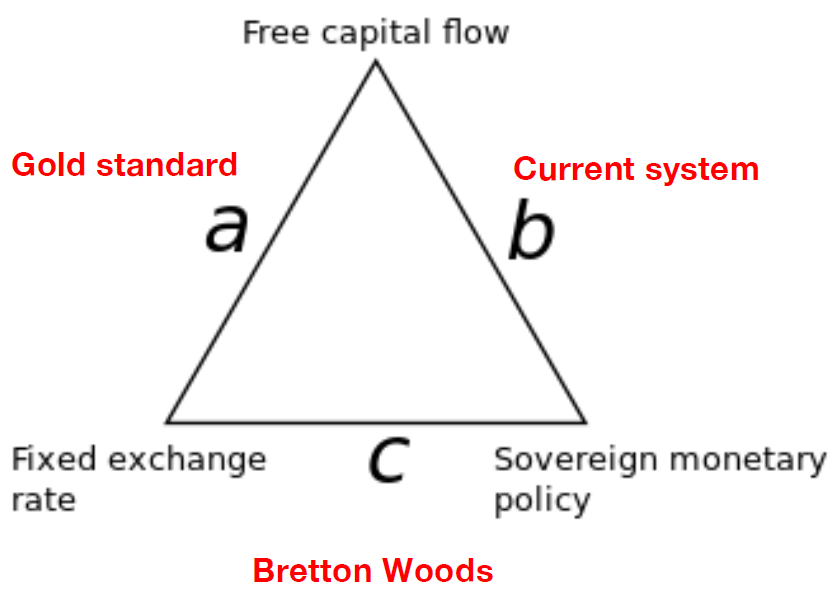
\includegraphics[width=\textwidth]{Pictures/trilemma.png}
\end{minipage}

\vspace{1\baselineskip}

Suppose a government wants to fight a recession by cutting its interest rates.
If capital can flow freely, this will result in a net outflow of capital in
search for a higher yield. This outflow will depreciate the currency - so you
cannot have a fixed exchange rate. Vice versa: If a government wants to fight
inflation by increasing its interest rates. If capital can flow freely, this
will result in a net inflow of capital in search for higher yield. This will
increase the value of the currency. You can only have two out of three:

\begin{itemize}
    \item \underline{Gilded Age}: Fix exchange rate and let money freely
        across the globe at the loss of an independent monetary policy.
    \item \underline{Golden Age}: Fix exchange rate and follow independent
        monetary policy at the loss of free capital flows.
    \item \underline{Fool's Gold Age}: Follow independent monetary policy and
        let money flow freely across the globe at the expense of a fixed
        exchange rate.
\end{itemize}

Bretton Woods is fully top-down steered, Gold Standard is fully bottom-up
laissez-faire, the current system is in the middle.

\subsubsection{Shifts}

\begin{itemize}
    \item When one structural economic regime passes into another, the economic
        system goes through a shift.
    \item Because each shift experiences the end of one era and the beginning
        of another, it always comes with geopolitical, financial and economic
        disruption and distress.
    \item However, during these shifts, also reform takes place, where the
        seeds are planted from which a new structural regime takes root.
\end{itemize}


\subsection{The First Shift (1911 - 1946)}

The first shift was characterised by nationalism, imperialism, war,
revolution, depression and genocide. There was huge unemployment.

\vspace{1\baselineskip}

Institutional reform with Roosevelt' New Deal (1933-1939):
\begin{itemize}
    \item \underline{Stabilizing the banking system} through bank reform acts
        (e.g. Glass-Steagall, establishment of the Federal Deposit Insurance
        Corporation - FDIC)
    \item \underline{Suspension of the Gold Standard}, with a freely floating
        US Dollar and increase of money in circulation by the Federal Reserve
    \item Increase \underline{transparency in the stock market} by mandatory
        publication of balance sheet, profit and loss statement\dots
    \item \underline{Public works and relief}: Hire unemployed to build schools,
        municipal buildings, waterworks, sewers, streets, parks airports, hospitals\dots
        (Civil Works / Public Works Administration)
    \item \underline{Social security act} establishing a permanent system of
        pensions, unemployment insurance, welfare benefits\dots
    \item \underline{National Labor Relations Act} guaranteed workers the
        right to collective bargaining through unions
    \item \underline{Fair Labor Standard Act} set maximum of 44 hours of work
        per week and minimum wages, child labor under 16 was forbidden
    \item \underline{Wealth Tax Act}: redistribute wealth by imposing a tax
        of 79\% on income over 5 million USD.
\end{itemize}

Wartime stimulus and massive capital investment during WW2:
\begin{itemize}
    \item The number of machine tools in the US doubled between 1940 and 1945.
    \item Almost all of these were paid for by the government.
    \item Because all were state-of-the-art, they could be reconverted to produce
        consumer goods after the war.
\end{itemize}

High-pressure economy of WW2 with 'infinite demand', created an environment
of 'Learning by doing' where everybody on all levels was eager to increase
efficiency and reduce costs. This working culture, adopted during the wartime
period, and the best-practices resulting from it, persisted after the war had
ended. As an example, in 1942, it took 8 months to build a standard Liberty
freighter ship, by the next year, this had been reduced to a few weeks.

\subsubsection{Bretton Woods}

In the summer of 1944 (3 weeks after D-day), 730 representatives of 44
countries gathered at the Bretton Woods conference with the ambitious goal
to redesign the international monetary system, the new system should:

\begin{itemize}
    \item replace the monetary chaos of the interwar period with a new
        international system that would support trade through stable exchange
        rates.
    \item Free trade was preferred to free capital flows, expecially to
        short-term 'hot money' flows and capital flight, and as such, it was
        explicitly recognized that countries needed to impose capital controls.
    \item Each country could still follow an independent monetary policy to
        fight recessions and stimulate employment.
\end{itemize}

Lessons would be learned from the past, and, more specifically from the
mistakes that had been made in the interbellum period where countries had
re-joined and then abandoned the gold standard following a beggar-thy-neighbour
strategy in a series of competitive devaluations. Protectionism had risen and
economic cooperation between the great powers had vanished leading to a
deepening and lengthening of the Gread Depression, which pushed many countries
into totalitarianism.

\vspace{1\baselineskip}

After the war, the idea rose to support trade through international cooperation,
but still be able to fight recessions with independent monetary policy. This
imposed capital controls.

\vspace{1\baselineskip}

After the war, "the Greenback was the only currency left standing and capable
of lubricating world trade".

\vspace{1\baselineskip}

Bretton woods established a system of payments based on the dollar, which
defined all currencies in relation to the dollar, itself convertible into
golt, and above all "as good as gold" for trade. US currency was now
effectively the world currency, the standard to which every other currency
was pegged.

\paragraph{Back to the trilemma of international finance}
The current system has the advantage that exchange rates can buffer an
economic shock, when a currency devalues, exports from that country become
very cheap. This is an alternative to devaluation through wage decreases.
However, free flow of capital creates flows of 'hot money'\dots see crises
of 1994 and 1997.

\paragraph{Lessons learned}

From the calamities during the first shift, lessons were learned from which
the Golden Age would rise:

\begin{itemize}
    \item Institutions were reformed \underline{to fight the Great Depression}.
    \item A social welfare system was installed \underline{to counter the
        upcoming Bolshevik revolution}.
    \item \underline{WW2} let to massive stimulus and capital investment.
    \item \underline{To fight nationalism}, and support trade in a balanced
        way, the international financial system of Bretton Woods was set up.
\end{itemize}


\subsection{The Golden Age (1947 - 1968)}

The two decades after WW2 were blessed with extraordinary economic growth:
\begin{itemize}
    \item Mean reversion: Recovery of the economy to its full potential
        after WW2.
    \item Stimulus: reconstruction of infrastructure and industry
    \item Productivity increase from technical innovations and capital
        investments
\end{itemize}

A social contract between workers and owners on
\begin{itemize}
    \item The parallel growth of real wages and productivity
    \item ensuring that the fruits of the economic progress were equitably
        shared
    \item Led to wealth accumulation and spare time $\Rightarrow$ CONSUMERISM
\end{itemize}

\paragraph{Inequality from the stone age to the 21st century}

"Thousands of years of history boil down to a simple truth: ever since the
dawn of civilization, ongoing advances in economic capacity and state
building favoured growing inequality but did little if anything to bring
it under control." Inequality will always have the natural tendency to increase,
only violent ruptures have been able to flatten it:

\begin{itemize}
    \item Mass mobilization warfare
    \item Transformative revolution
    \item State failure
    \item Lethal pandemics
\end{itemize}

\paragraph{Consumer Society}
Free time and wealth accumulation created a consumer society with new demand
for consumer goods like electrical apparel, automobiles or entertainment
services.

\paragraph{The Rise of hydrocarbon man}
During the Gilded Age, coal has been the primary energy source. During the
Golden Age, Oil and Natural Gas have been added to mix and taken up a bigger
proportion. The West becape very much dependent on fossil fuels.

\paragraph{The Fall}

"The Great Society rests on abundance and liberty for all. It demands an end
to poverty and racial injustice\dots The Great Society is a place where every
child can find knowledge to enrich his mind and to enlarge his talents\dots
It is a place where the city of man serves not only the needs of the body and
the demands of commerce but the desire for beauty and the hunger for cummunity."
changed to "Things fall apart, the center cannot hold. Mere anarchy is loosed
upon the world\dots" Anarchy and countercultures emerged.


\subsection{The Second Shift (1969 - 1979)}

\paragraph{The Nixon shock and the end of Bretton Woods (1971)}

\begin{itemize}
    \item The Bretton Woods system was based on trust in the US Dollar.
    \item But the US overstreched in a Vietnam war combined with rising
        public expenditures in the Great Society programs
    \item At a certain point there were more dollars in the hand of foreign
        countries (so-called eurodollars) then the total gold stock of the US
    \item Trust in the US Dollar, which was the keystone of the Bretton Woods
        system, evaporated
    \item In February 1965, President Charles de Gaulle sent the French Navy
        across the Atlantic to pick up the French reserve of gold, a gesture
        which was soon followed by other countries.
\end{itemize}
As long as the US had a trade surplus, all the dollars it was sending out,
came back. When reversed, the Eurodollar pool became a lake and a sea. The
world was awash with dollars that were all supposed to be backed by Gold.

\begin{itemize}
    \item The US gold reserves, which were at 65\% of the world monetary stock
        in 1952, reduced to 29\% in 1967, 15 later.
    \item The opposite happened in Europe, where the combined gold reserves
        of France, Germany and the UK were at 6\% of global stock in 1952,
        increasing to 26\% in 1967.
    \item This dynamic ended on August 15, 1971, with the 'Nixon Shock', when
        the US President Richard Nixon unilaterally ended the convertibility
        of the Dollar to gold. This was the end of the Bretton Woods system.
\end{itemize}

\paragraph{Peak Consumption}
You can only buy a limited amound of stuff, technology adoption follows
the S-shape of the logistic growth process, where the strongest growth
rate can be observed during the Golden Age.

\vspace{1\baselineskip}

Economic paradigm shift from falling unemployment with rising inflation,
to stagflation. Fiscal and monetary overstreching because of Lyndon Johnson's
Great Society and the Vietnam war.

\paragraph{Philips' Relation}
Intuition: A falling unemployment rate signals an increase in the demand
for labor, which puts upward pressure on wages. Profit-maximizing firms then
raise the price of their products in response to rising labor costs.

\vspace{1\baselineskip}

From the end of the fifties, throughout the sixties, many economists were
convinced that there was a fundamental and permanent relationship between
inflation and unemployment. It was conjectured that the process underlying
this 'law of nature' was based on a virtuous cycle where higher demand for
goods would increase prices, which in turn would encourage companies to hire
more personal, increasing general employment, and again driving up demand
in a positive feedback loop. This relationship, called the \fat{Phillips
curve}, was one of the empirical backbones of Keynesian policy. It was believed
that governments could make a trade-off between inflation and employment.
Government spending and tax reductions could be used to stimulate the economy,
which would have inflationary effects. However, a reasonably high level of
inflation would be acceptable as this would lead to a lower unemployment through
the Phillips relationship. As such, it was believed that governments could
spend their way out of a recession by cutting taxes and boosting government
spending. Any inflation that would come as a by-product of this policy would
be politically acceptable as it would result in higher employment through
the Phillips curve.

\vspace{1\baselineskip}

In the beginning of the 1970s, western countries started losing their grip
on oil exploitation, this let to 2 oil shocks:
\begin{itemize}
    \item Firs oil shock with the OPEC oil embargo as a reaction to the
        Yom Kippur war (1973 Arab-Israel war)
    \item Second oil shock with the Iranian revolution under the leadership
        of Ayatollah Khomeini (December 1978 / January 1979)
\end{itemize}

The most dramatic knock-on effect that would lead to the first oil shock and
as such would contribute to the global power shift in oil markets, came about
in October 1973, when a coalition of Arab forces, led by Egypt and Syria
launched a surprise attack on Israel on the Jewish holy day of Yum Kippur,
the Day of Atonement. The Yum Kippur war lasted only three weeks, featured by
intense fighting with one of the most spectacular reversals in military
history, when the Israelis managed to turn around a hopeless situation 'from
being within hours of extinction to shattering the invadeing forces and advancing
on Damascus and Cairo'. The fact that the Americans had supported the Israeli
forces with military supplies, in a very plain and unsophisticated fashion, at
crucial stages during the three-week period of hostilities, bonded the alliances
within OPEC.


\subsection{The Fool's Gold Age (1980 - \dots)}

\paragraph{The Illusion of the Perpetual Money Machine}

\begin{itemize}
    \item Consumption, not funded by savings but by debt, and by wealth
        extracted from the stock and the housing market
    \item Economic growth, not driven by productivity increase in the real
        economy, but by growth of the financial sector
    \item Further supported by a climate of deregulation and a massive
        growth in financial derivatives
    \item Resulting in a succession of bubbles and crashes, feeding upon
        each other and culminating in the GFC (Global Financial Crisis) of
        2008
\end{itemize}

The ultimate financialization offered by ETFs opens the road to more
bubbles created by the herding mechanism of small investors as well
as large hedge funds and sovereign funds crowding in and out of the
investment fashion of the moment.

\paragraph{Reaganomics / Thatcherism}

\begin{itemize}
    \item Decline in Representation: Decline in Union Membership
    \item Reagen decreased taxes of the rich to provide an incentive to
        save. This would increase investment and create jobs.
    \item The savings of the rich would 'trickle down' to the masses.
\end{itemize}

The sharp rebound in inequality in the US was mainly the result of a shift in
economic policy often referred to as 'Reagonomics' or 'Thatcherism'. John
Komlos, Professor Emeritus at the University of Munich, describes the ideology
of that time as follows: In short, Reagen advocated decreasing the taxes
of the deserving rich, which would provide incentives to increase savings
and investment and thereby create jobs and subsequently 'trickle down' to
the masses so they will benefit from it in due course. Moreover, lower taxes
meant an increase in take-home pay and that would provide an incentive for
people to work harder and for entrepreneurs to take more risk, thereby growing
the economy and boosting incomes.

\begin{itemize}
    \item The fruits of economic growth not equitably shared
\end{itemize}

Method was a bit counterproductive. The rich got ver richer and the poor
only got a little bit richer. The gap increased.

\paragraph{Decreasing Savings, increasing consumption based on debt}

Consumption was paid with debt.

\paragraph{Stock Markets}

The Fool's Gold Age was characterized by a very strong stock market
performance, with lagging earnings. This strong stock market performance
is not reflected in an increase in productivity. To the contrary we see
a secular decline in the productivity in the West over the past 50 years.

\paragraph{Economic Growth}

There is a different picture for China. China paints a completely different
picture with a very strong increase in per capita real GDP over the past 40
years.

\subsubsection{Three waves of globalization}

Globalization is not an inevitable process, and it is also not a linear
process.

\begin{figure}[h]
    \centering
    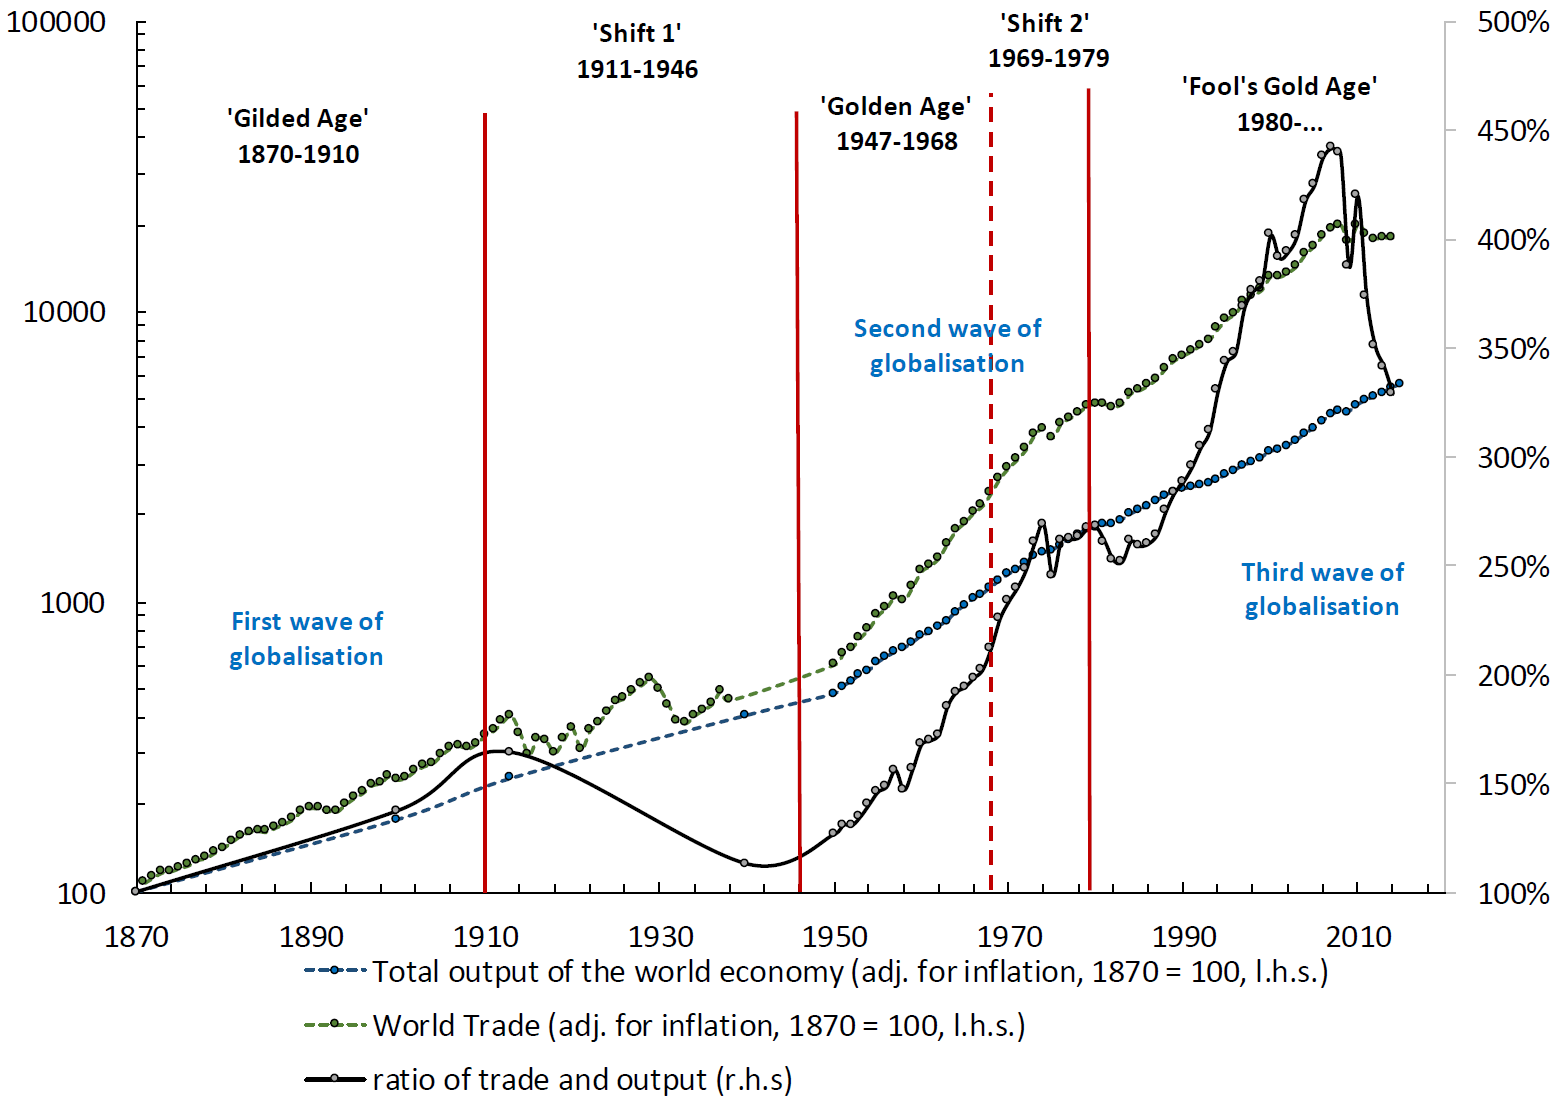
\includegraphics[width=0.6\textwidth]{Pictures/three_waves_of_globalization.png}
\end{figure}

\begin{itemize}
    \item The first wave came with the technological revolution, pushed
        forward by increasing connectivity, falling transportation costs
        and the gold standard and the Pound Sterling that create a global
        marketplace.
    \item The second wave: Renewed international cooperation and trade
        liberalization after nationalism during the First Shift brought
        globalization back to its previous level. But flows between
        emerging and developed markets were limited to those primary
        commodities that did not compete with agriculture in the developed
        countries.
    \item In the third wave, new information and communication systems made
        it possible to manage and control geographically dispersed supply
        chains. Production flowing to places with lower cost of labor.
\end{itemize}

\paragraph{The second vs third wave of globalization}

\begin{itemize}
    \item In the second wave of globalization, resources were extracted
        from developing countries. Trade flows were mainly raw materials
        from developing to developed countries.
    \item In the third wave, developing countries were integrated in the
        global supply chains.
    \item The second wave mainly favored the rich countries. During the
        third wave developing countries made a spectacular catch-up movement.
\end{itemize}

\paragraph{The Economic center of gravity is moving East}

The Economic gravity an dlight mean centre moved to the east.

\paragraph{Debt, Investment, Financialization and Consumption in the Fool's Gold Age}

\paragraph{Debt}

Another characteristic of the Fool's Gold Age is the massive increase
in debt, but the remarkable decrease in the 'efficiency of debt'.
Now one dollar in the non-financial sector 'generates' $25$ cents in
GDP. Student loans and Car loans increased immensly.

\paragraph{Investment}

But this increasing in debt is not used to increase investment in tangible
assets.

\paragraph{Consumption}

Consumption has still increased since the Golden Age, but the mix has shifted
from goods to services (healthcare, pension, financial services, insurance)

\paragraph{Financialization}

Massive growth of the derivatives market up to a current level of $600-700$
trillion USD.
Rise of machines: automatic trading / high-frequency-trading.

\begin{itemize}
    \item Put simple, ETF's are funds that are traded on the stock market
        (ETF = Exchange Traded Funds).
    \item ETFs can specialize in certain investments e.g. gold, or oil,
        or other commodities.
    \item They provide a very easy access for smaller investors to specific
        products, or stategies.
    \item There are now 5 Trillion USD in ETFs outstanding.
    \item Massive growth of the ETF industry.
\end{itemize}


\subsubsection{ETF impact example: Negative oil prices}

What are oil futures?
\begin{itemize}
    \item Futures are standardized contracts between a seller and a buyer
        for the delivery (of oil) at a specific time in the future.
    \item There are future contracts for each month in the future up to
        many years ahead, but the further out the less liquid the
        contract becomes.
    \item Each future contract has its own price evolution, normally,
        the correlation between the contracts will be high, but there
        may be substantial differences nevertheless.
    \item Producers and big consumers of oil use futures contracts to lock
        in a future price to buy or sell the product that they need
    \item If you want to invest (speculate) in the oil (commodities) market,
        you cannot accept physically delivery of the product, then you have
        to buy a future contract.
    \item A graph representing prices as a function of the delivery date
        (x-axis) is called the term structure
    \item If the graph is upward sloping, it is said that the market is
        'in contango'
    \item If the graph is down sloping, it is said that the market is 'in
        backwardation'
    \item If you buy one of these futures contracts, you are obliged to buy
        1000 barrels of WTI Crude Oil at the contract/delivery date.
    \item If you cannot accept this physical delivery, you have to 'sell'
        your contract in time before the settlement date.
    \item This can be at any price, and, as we have seen on April 21 2020,
        even negative prices.
    \item Longer term investors always sell the futures contract before
        the settlement date and use the proceeds to enter a new contract.
        If the market is in contango this results in a loss, if the market
        is in a backwardation it results in a profit.
    \item This is called 'rolling'
\end{itemize}

\begin{figure}[h]
    \centering
    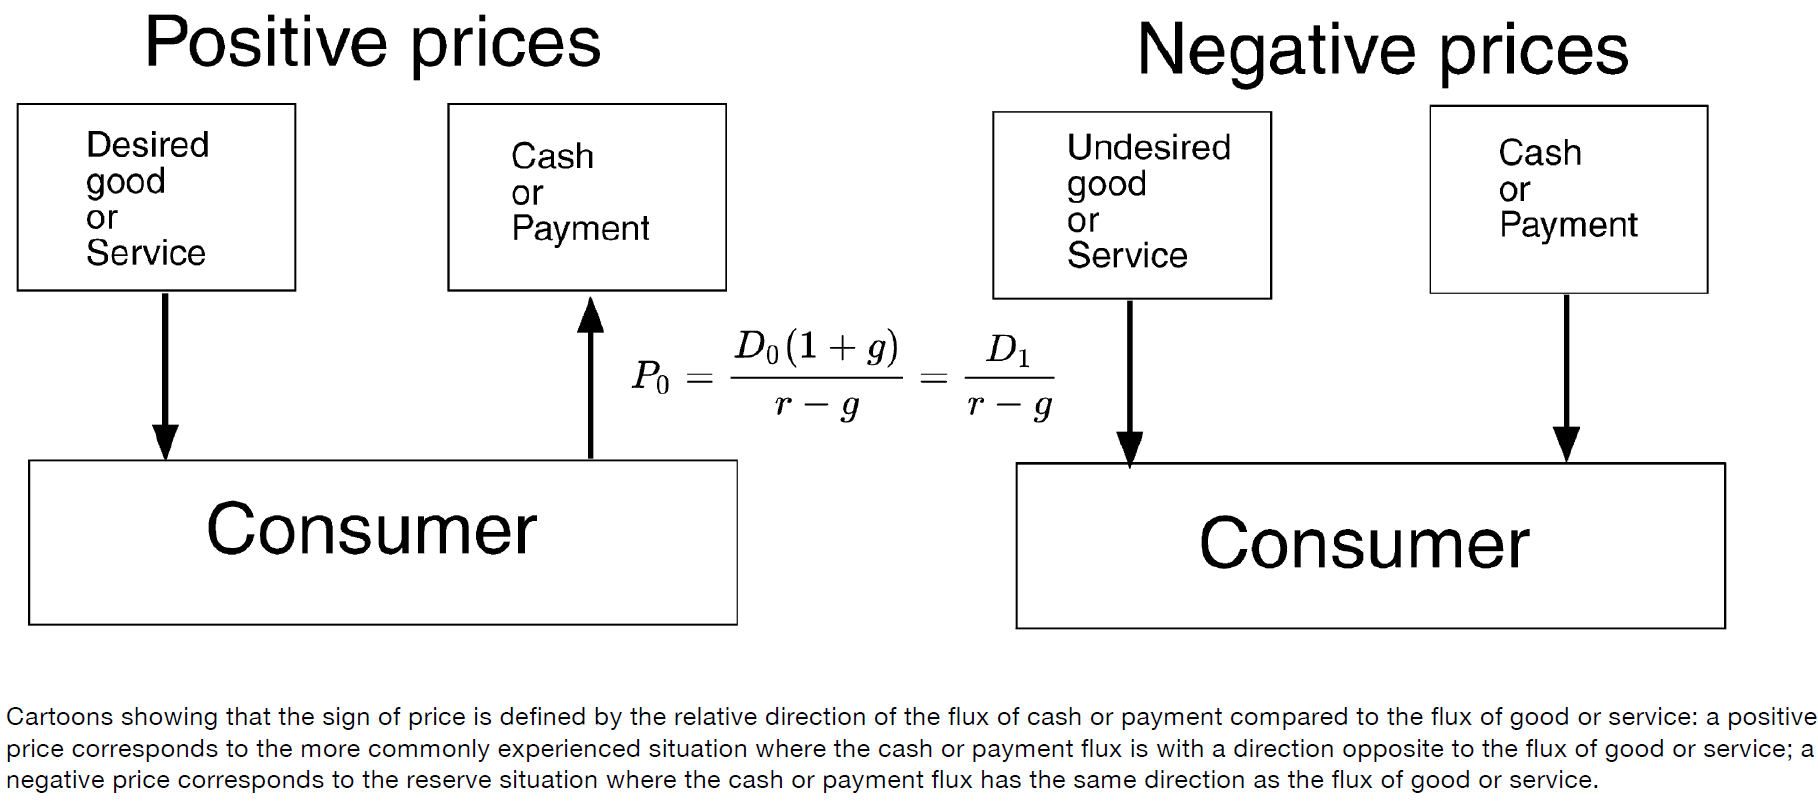
\includegraphics[width=0.9\textwidth]{Pictures/Price_sign.png}
    \caption{Price sign}
\end{figure}

\begin{itemize}
    \item For retail investors, future are not very convention because
        you need to buy 1000 units in one contract.
    \item That is where ETFs come in handy.
    \item Those are stock listed companies that e.g. for oil only buy oil
        futures. You can buy a share in that company on the market e.g. for
        the ETF USO (US oil) you can buy shares at the price of a few USD
    \item An ETF like USO does not want physical delivery and has to roll
        its positions before the settlement date.
    \item With the existing super-contango in oil, this resulted in a monthly
        loss of $33\%$ at the end of April 2020
    \item Over the month of April $2020$ there has been outsized inflow
        (3 Bn USD) in the United States Oil Fund (ETF)
    \item The fund has to roll its future every month and even publishes its
        "roll dates" (when it is selling the near month contract and buying
        the next month contract)
    \item So, between 7/04 and 13/04, 2020, USO had to 'roll' 4 Bn USD of
        oil futures from the front contract to the next.
    \item With this size, USO totally dominated the market of the front
        (selling) and the next month (buying) futures
    \item Because the flows of USO were predictable, many 'professional
        investors' did front running on the ETF
    \item Frontrunning means that they took a position ahead of a large order,
        taking profit from the market impact of that order.
    \item They knew that the front contract would go down, and the next
        contract would go up (relative to each other), so they shorted
        the front and went long the next.
    \item This massive short position on the front contracts hat to be
        closed before April 21. But there were only sellers and no buyers,
        this resulted in a price drop of $-300\%$ on April 20.
    \item The market hat to go in negative territory ($-40$ USD) to find
        "buyers" of the front WTI future contract.
    \item Negative prices were only seen in the front contract. For example,
        if you look at the 6M ahead contract of OCT 2020, you could see a
        large drop from 31 to 25, which is a $20\%$ drawdrop on the same
        day (but not a $300\%$ crash).
\end{itemize}

\paragraph{Bubbles feeding upuon each other in the Fool's Gold Age}

Examples: Black Monday (October 19th 1987), Dotcom Bubble (March 2000),
House price bubble peaking mid-2006

\vspace{1\baselineskip}

The historical evolution of the S\&P500 Index showing the price growing faster
than an exponential up to its tipping pint of 19th October 1987. The dotted
and solid smooth black lines are the results of our model calculations with
two different levels of nonlinearity. Reproduced from the book "Why stock
markets crash" by D. Sornette

\vspace{1\baselineskip}

Quaterly average House Price Index in the 21 states and in the District
of Columbia (DC) where Zhou and Sornette diagnosed bubble-type behaviours in
June 2005 and predicted a peak in mid-2006. For comparison, the HPI has
been normalized to 100 at the second quarter of 1992.

\vspace{1\baselineskip}

US real house prices between 1974 and 2014. Threee peaks in the growth
rate are immediately followed by a correction. When the growth rate itself
grows, the process becomes unstable and a correction follows around the
critical point embedded in the faster-than-exponential growth process.

\subsubsection{Bubble of everything 2007}

\paragraph{Stocks}
The historical evolution of the S\&P500 index shown as dots. The
dashed vertical line shows the last observation used to calibrate our model.
The colored curves show different fits. It is expected that the correction
occurs with 80\% probability in late 2006. This indeed happened.

\paragraph{Oil}
Also crashed mid-2008.

\paragraph{Debt} Bubble also burst.

\paragraph{Globalization Bubble}

The time series represent a proximity index of emerging markets equities
and currencies, freight prices, soft commodities, base and precious metals
and energy.

\subsubsection{Central bank policies as slaves to the stock market}

Federal fund rates are consistently cut after stocks decline. Do central
banks have an unofficial mandate to support stock markets?
The key question, however, is this: did it lead of lag? According to common
wisdom and standard textbook arguments, a decrease of interest rates is
supposed to make borrowing cheaper. This results in increasing expectations
of future growth. Additionally, lower rates mean lower discount factors.
The combined effect should be a boost on stock prices. In this line of
reasoning, a federal funds rate decrease should lead economic growth and
cause stock market prices to increase. This, anti-correlation and a lead
of the Fed rate are expected.

\paragraph{"Primum non nocere" vs the illusion of control}

In the US, there is a zero-tolerance, with the objective to stop all fires.
In Mexico, there is a laissez-faire policy, arguably due to weaker resources
and smaller loss exposure. The results are drastically different: while
Southern California has few small fires, extremely large fires are shockingly
frequent; In contrast, Baja California is graced with many small and essentially
no large fires.

In order for the system to be resilient against catastrophic events, deadwood
needs to be cleared in a natural, dynamic, self-organized way. Could this
observation also be true for the economy? With the special actions that
central banks have been carrying out since the crisis, are we not piling up
deadwood, with the zero-tolerance practice?

\begin{figure}[h]
    \centering
    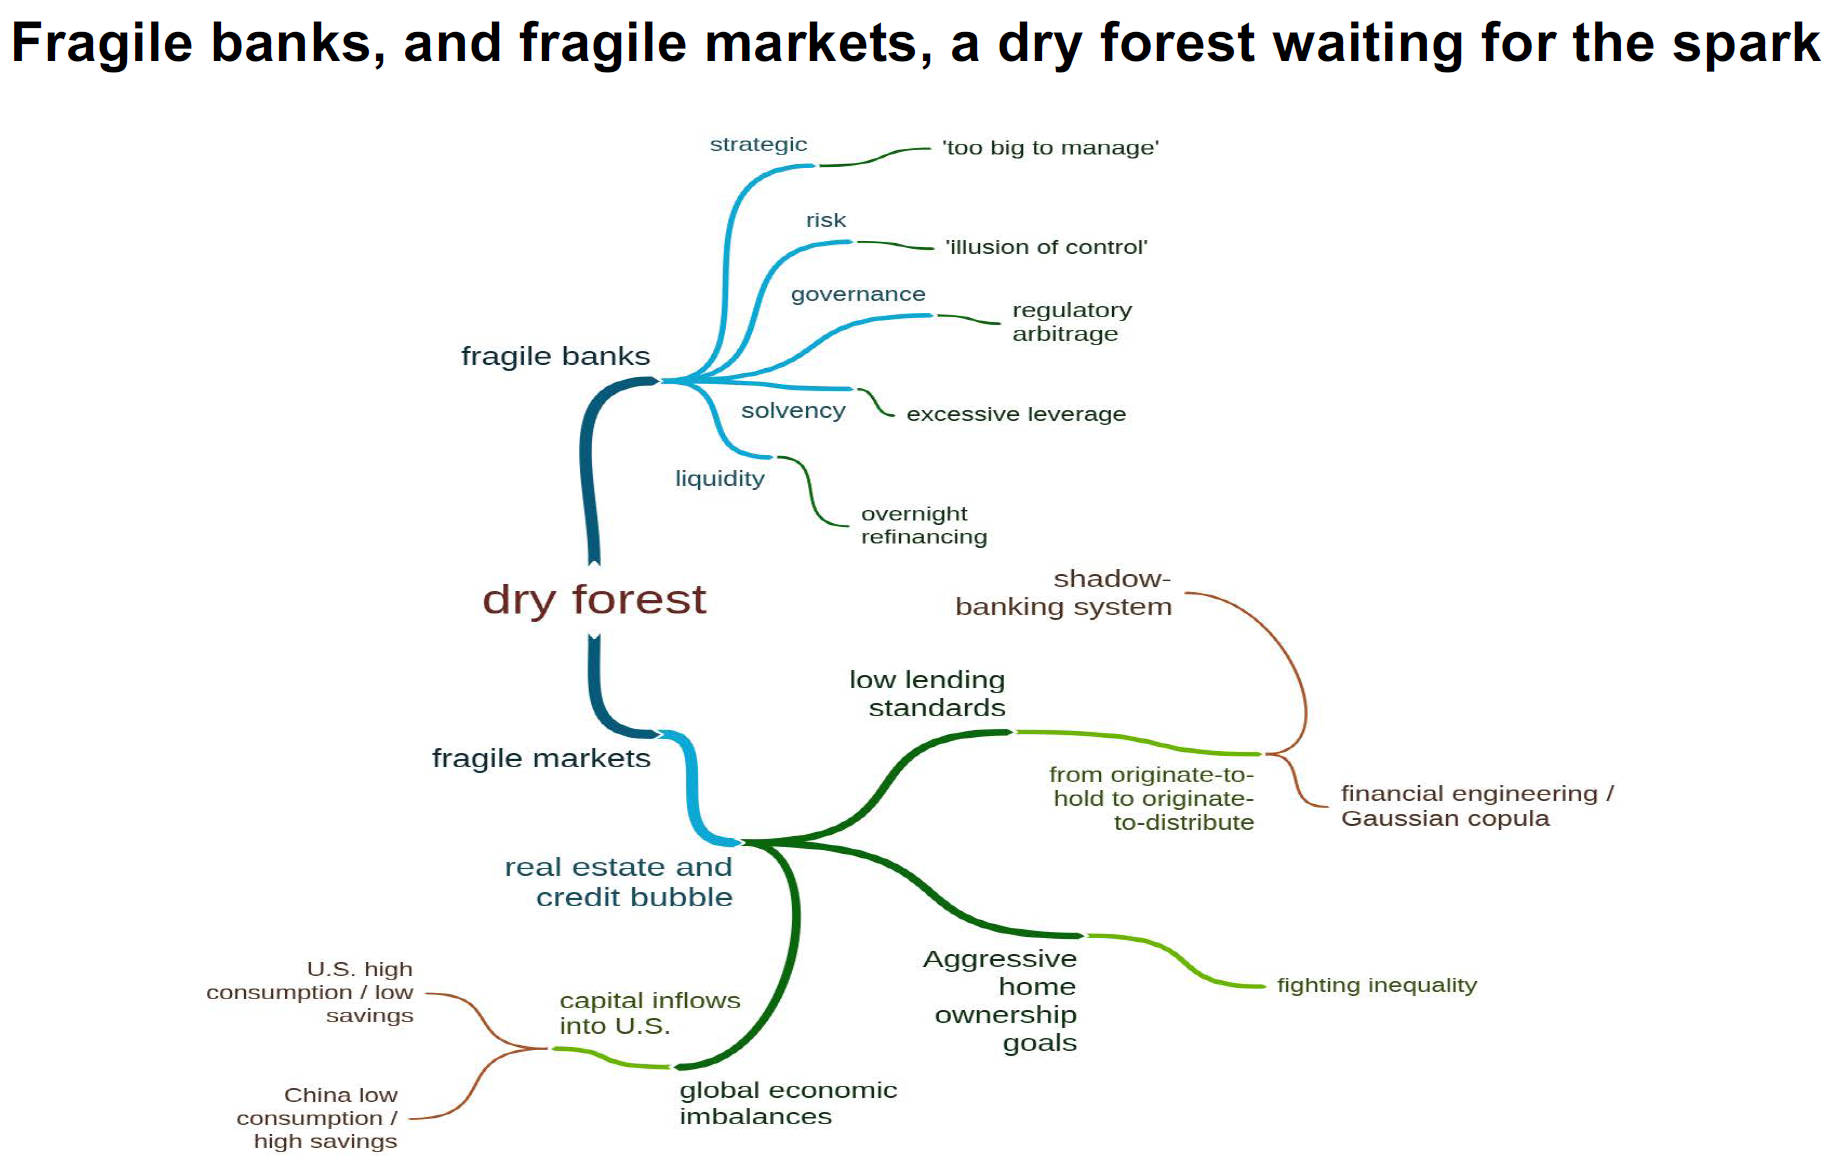
\includegraphics[width=\textwidth]{Pictures/dry_forest.png}
\end{figure}

\subsection{Conclusion}

\paragraph{The super-business cycle - a 150 year endogenous view on
economy and society}

We have described the three economic regimes and the two shifts of the
super business cycle of the past 150 years.

It is important to stress that we view this cycle as endogenous. Boom
and burst are two sides of the same coin. It is a fundamental property
of capitalism to cycle through periods of optimism and pessimism. Periods
of growth have the tendency to overshoot. This is naturally corrected in a
phase of consolidation or even decline.

This is in stark contrast to the exogenous view, thwre recessions are seen
as a symptom of disease, caused by some external factor that needs to be
eradicated or modified for the system to be cured.

According to Hyman Minsky, capitalism has evolved, since the late nineteenth
century, through a super-financial business cycle with four stages.

\begin{itemize}
    \item Commercial
    \item Finance capitalism
    \item Managerial Welfare state capitalism
    \item Money manager capitalism
\end{itemize}

\paragraph{Commercial capitalism}

\begin{itemize}
    \item In 'Commercial Capitalism' the financial system was centered
        around commercial banks.
    \item Banks financed working capital, in the form of short-term loans,
        to cover operational expenditures and the purchase of materials
        necessary in the production process.
    \item Long-term investments were financed from retained profits, or
        from equity injected by the owners.
\end{itemize}

\paragraph{Finance capitalism}

The second industrial revolution drastically changed the system:
\begin{itemize}
    \item With the industrialization of the production process and the
        need to build big infrastructure came the strong demand for the
        long-term finance of capital expenditure (CAPEX).
    \item Finance became globalized as stocks and bonds, issued to service
        long-term capital investment, were sold in international finance
        markets.
    \item The financial system became dominated by investment banks.
\end{itemize}

'Stability is destabilizing ' (Minsky):
\begin{itemize}
    \item In a boom, financial institutions innovate to bypass rules and
        regulations imposed by the supervisory authorities.
    \item By the 1920s, investment banks were largely devoting their efforts
        to financing speculation in financial assets. As such, 'financial
        capitlism' ended in the crash of 1929, which ultimately led to
        the Great Depression.
\end{itemize}

\paragraph{Managerial welfare capitalism}

\begin{itemize}
    \item After the 1929 crash and during the Great Depression, the
        pendulum swung back. The financial sector was reformed with
        the New Deal legislation and the federal government took up
        a bigger role in managing the economy.
    \item Following the transition period, this corresponds to the Golden
        Age of stable economic growth, high employment and a social
        contract between workers and owners which guaranteed rising
        wages and low or even decreasing inequality.
\end{itemize}

Again 'Stability destabilized' (Minsky):
\begin{itemize}
    \item The absence of deep recessions and severe financial crisis
        encouraged innovations that increased instability.
    \item New Deal reforms were cut back
    \item The financial system was again deregulated (Glass-Steagall)
\end{itemize}

\paragraph{Money manager capitalism}

\begin{itemize}
    \item The Golden Age created large pools of savings (e.g. through
        increased prosperity, Petrodollars\dots)
    \item From this, the 'shadow banking system' was born (pension funds,
        asset managery, mutual funds, hedge funds, sovereign wealth funds,
        private equity funds and university endowments)
    \item The 'reason for existence (raison d'être)' of this type of capitalism
        it to manage huge pools of capital in search of the highest return.
    \item The financial system no longer serves the productive economy but
        serves only itself; the snake bites its own tail.
    \item The innovation and exploration process started focusing on the
        financial sector itself.
    \item This is what we call financialization, which led to a massive
        growth in complex financial derivatives.
\end{itemize}


\begin{figure}[h]
    \centering
    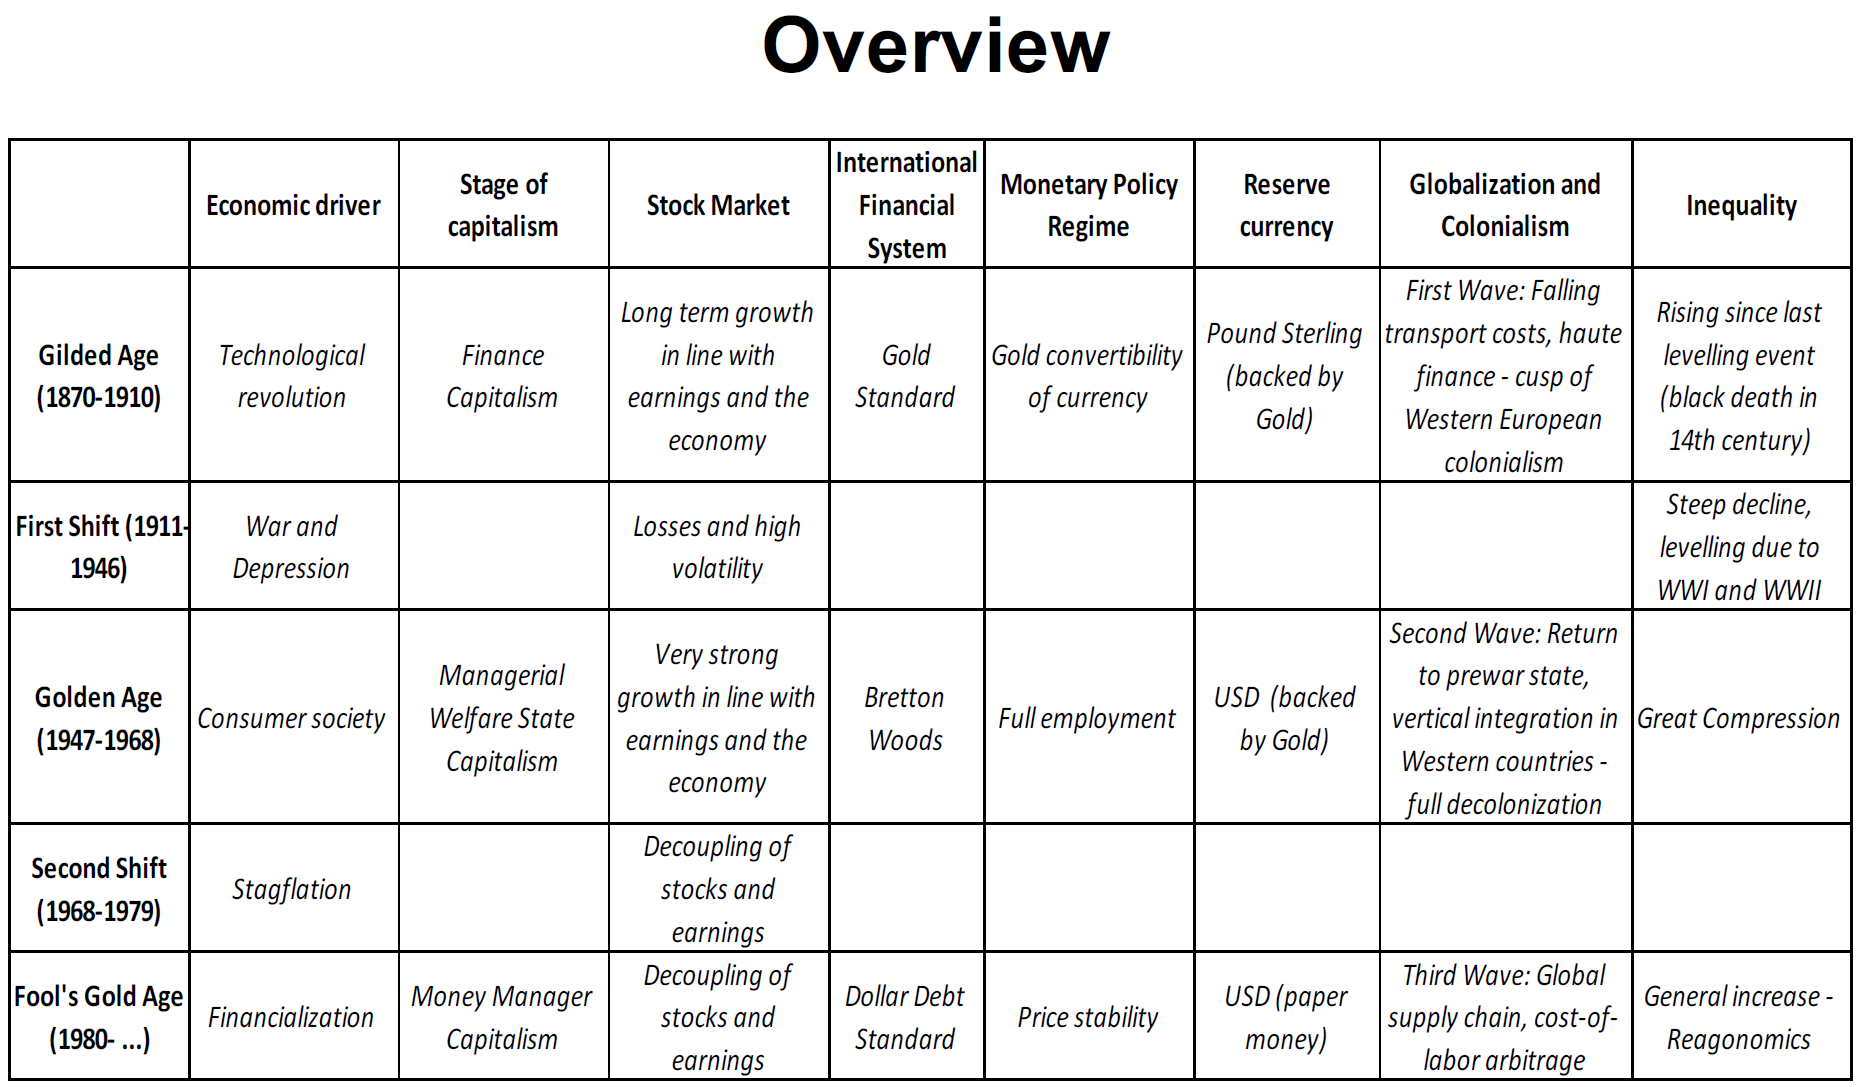
\includegraphics[width=\textwidth]{Pictures/6_Overview.png}
    \caption{Overview}
\end{figure}

\paragraph{A glimpse into the future?}
\begin{itemize}
    \item The Fool's Gold Age has been ongoing for almost three to four
        decades.
    \item I think that around 2008-2019, we have transitioned into a new
        Shift (2020-2050)
    \item The new shift is characterized by many challenges.
\end{itemize}

\paragraph{The future of public debt}
Governments are accumulating debt in an ever-increasing spiral:
\begin{itemize}
    \item GFC (2009)
    \item European Debt crisis (2011)
    \item Covid-19 (2020) and the current multi-trillion stimulus package
\end{itemize}
On top of that there are:
\begin{itemize}
    \item Rising pensions
    \item Healthcare costs
    \item Aging population
\end{itemize}
Towards a new definition of money, direct monetary financing or a debt
jubilee? Chinese DCEP (digital currency electronic payment)

\paragraph{Covid-19 stimulus - how much further can this go?}

\begin{itemize}
    \item \underline{The economist}: At least \$8trn of state loans and
        goodies have been promised to private firms in America and Europe,
        roughly equivalent to al their profits over the past two years. But
        there is still no guarantee that this mountain of money can prevent
        chaos.
    \item \underline{The FT}: Total worldwide stimulus announced since 2020
        comes to about \$14tn, according to the IMF, after adding various
        government spending packages. Such activity has given a big lift
        to asset prices, from stocks to junk bonds.
\end{itemize}

\begin{figure}[h]
    \centering
    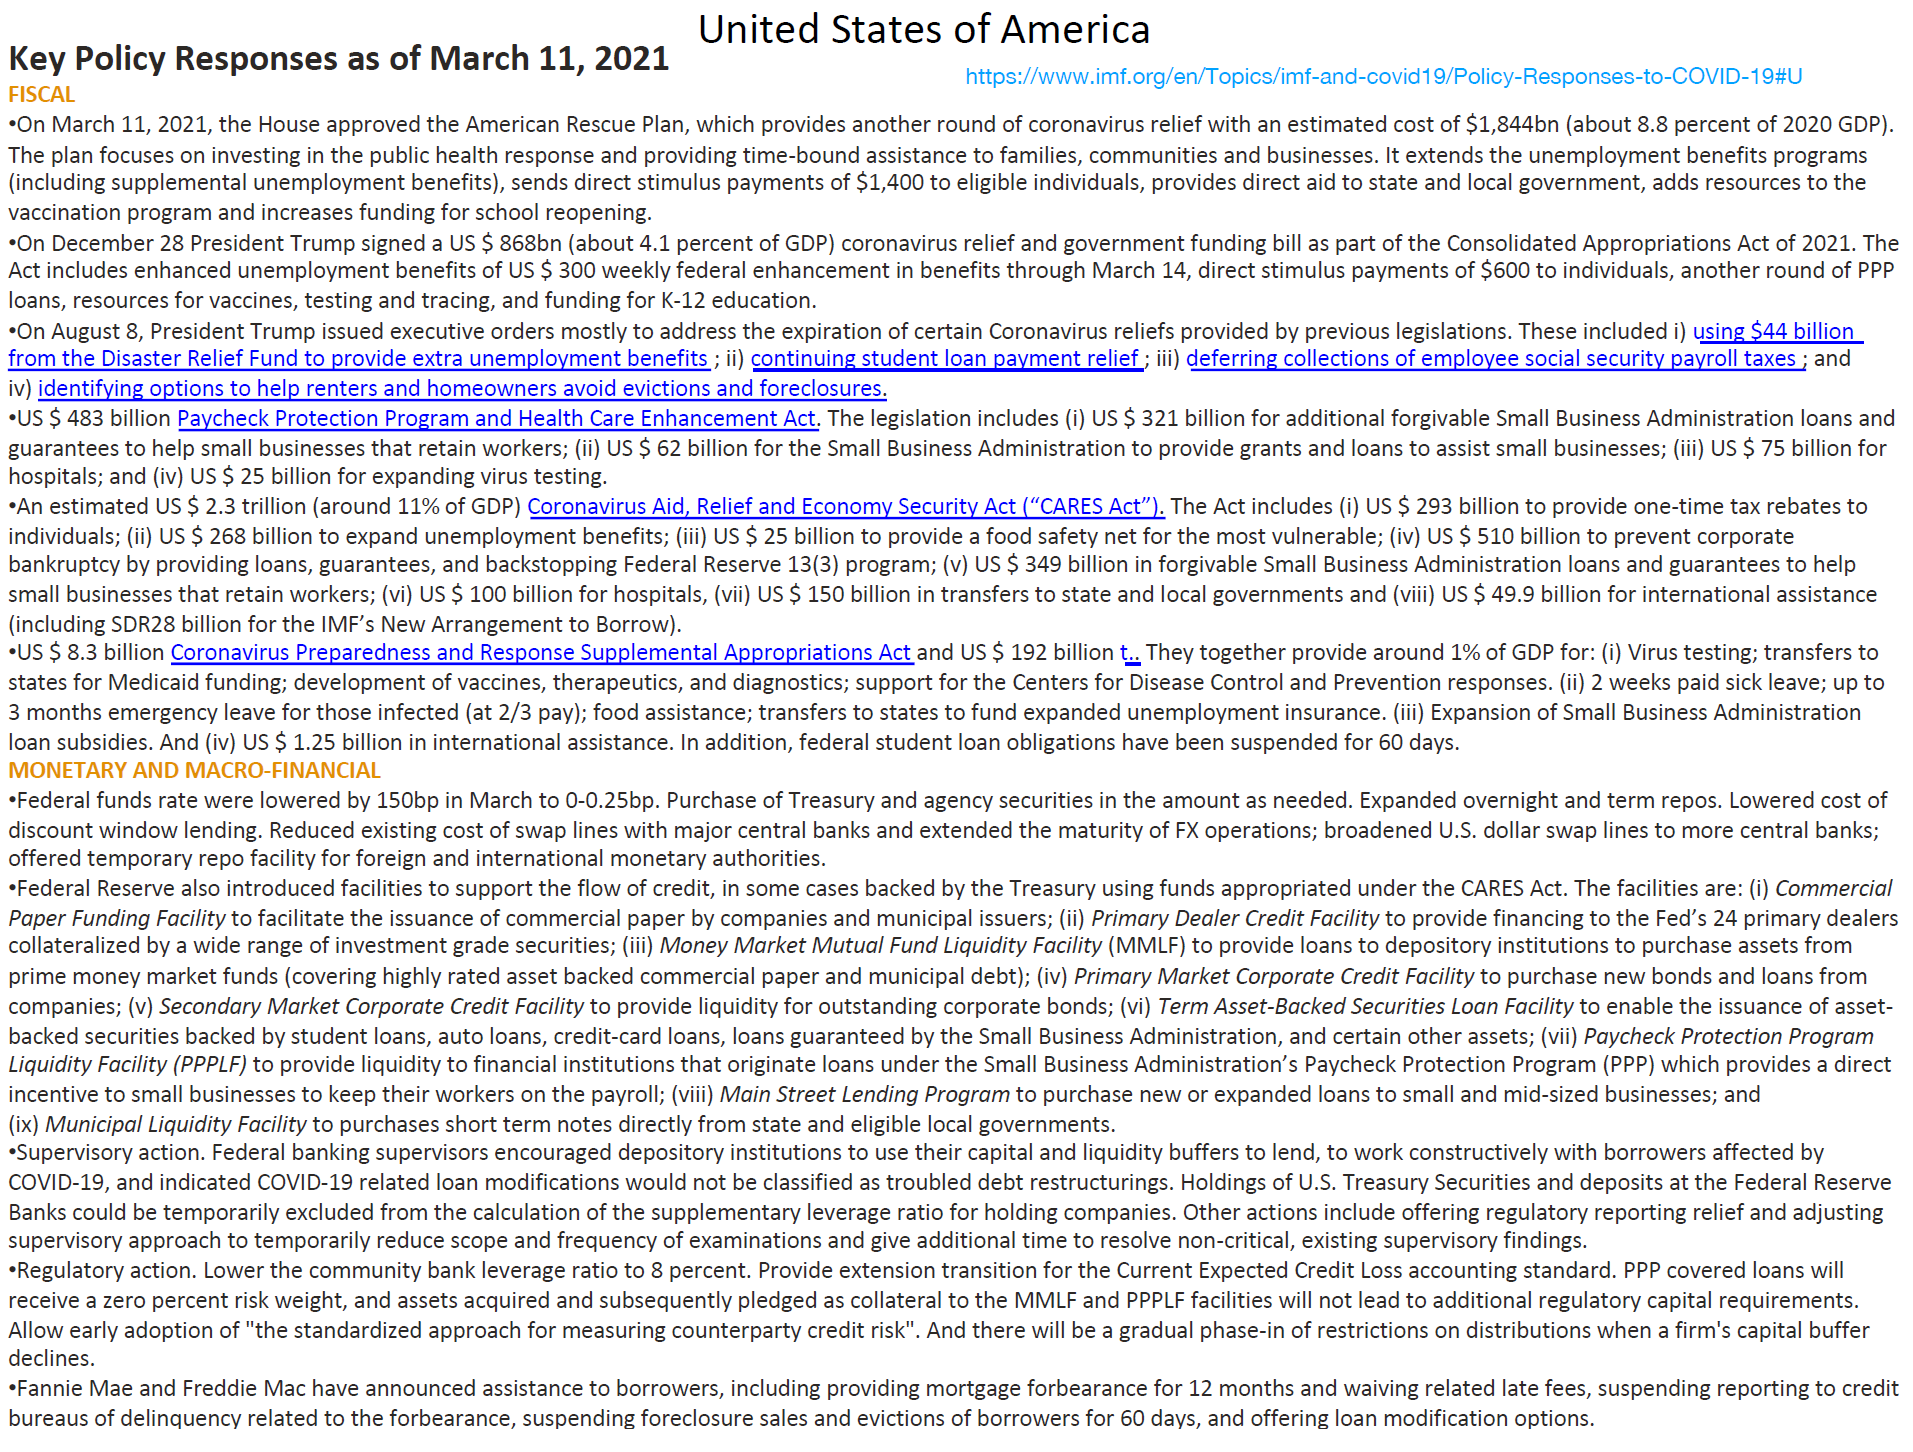
\includegraphics[width=\textwidth]{Pictures/Covid_USA.png}
    \caption{Key policy responses to Civid-19 in the USA}
\end{figure}


\subsubsection{A new bipolar world with two great "empires"?}

With the White House continually provoking tensions against Russia and Chine,
the doyen of American foreign policy, Henry Kissinger, dramatically warned
Washington last week to either agree to a new international system or continue
pushing tensions that are leading to a situation similar to the eve of WW1.

\begin{itemize}
    \item The economy converged with the US at the fastest pace on record.
        China's GDP was $71.4\%$ of US levels in 2020, according to the
        International Monetary Fund, up $4.2\%$ from the previous year
    \item The share of global trade increased as pandemic-related exports
        surged. Already the world's top exporter, China's shipments increased
        $3.6\%$ in 2020, according to official data. Total world trade likely
        contracted $5.6\%$, according to estimates from the United Nations'
        trade and development body UNCTAD
    \item China likely regained the title as the world's top destination for
        foreign investment, which it lost to the US in 2015. Foreign investment
        into China reached more than $\$129.5$ billion through November 2920,
        slightly above the previous year. Globally, FDI flows are likely to have
        fallen $30-40\%$ year-on-year in 2020, according to UNCTAD
    \item The Fortune Global 500 list of the world's largest companies by
        revenue for the first time contained more companies based in China,
        including Hong Kong, than the US: $124$ vs. $121$.
    \item Full-year movie box office receipts overtook the US for the first
        time.
    \item Sovereign debt was added to the FTSE Russel benchmark index,
        completing the country's inclusion in all three top global bond
        indexes. Foreign investors bought $1.1$ trillion yuan (\$ $170$
        billion) of Chinese bonds in 2020.
\end{itemize}

Kishore Mahbubani is a Singaporean civil servant, a career diplomat and an
academic. During his stint at the Ministry of Foreign Affairs from 1971 ot
2004, he served as Singapore's Permanent Representative to the UN and held
the position of President of the UN Security Council between January 2001
and May 2002. Between 2004 and 2017, he served as Dean of the Lee Kuan Yew
School of Public Policy at National University of Singapore.

\vspace{1\baselineskip}

US Army General H.R. McMaster expressed the american attitude succinctly:
"At the end of the day, the struggle between America and China represents
the struggle between 'free and open societies and closed authoritarian
systems.'" And just like the Soviets, the Japanese or the Nazis before them,
this new "authoritarian" challenger, i.e. Chian, barely stands a chance
against America, the de facto torchbearer of Western civilisation.

\vspace{1\baselineskip}

Except this time, as Mahbubani convincingly contends, the choice is not that
straightforward. Burgeoning student debt, housing crisis, an ongoing opioid
epidemic, a poor healthcare system, crumbling infrastructure - these are
tell-tale signs of an empire in decline. Even more striking is the yawning
gap between public policy and public opinion. Mahbubani cites several
credible research papers which document the broad convergence of opinion
among academics that policymaking in US is largely dominated by an increasingly
small economic elite while the average American has little to no say. And
while self-correction is baked into democratic institutions, they to not have
the leeway to make major U-turns in a short timeframe.

\vspace{1\baselineskip}

Big issues: Uighur humanitarian crisis and the Xinjiang separatist movement,
Tibet, Taiwan, Hong Kong, \dots

\paragraph{Pollution, climate change, biodiversity loss}

The big challenge is to develop countries without crossing a sustainability
threshold.

\paragraph{However\dots}

\begin{itemize}
    \item We showed, that regime shifts in society, economy, culture and
        technology are the natural phenomenon.
    \item In the past $150$ years we have seen $2$ shifts and $3$ structural
        regimes.
\end{itemize}

We have seen that revolution, war, depression, genocide, nationalism during
the First Shift let to a response of statesmanship, international cooperation
and fairness (equity):
\begin{itemize}
    \item Institutional reforms (e.g. Roosevelt's New Deal)
    \item International cooperation (e.g. Bretton Woods)
    \item A society contract between owners and workers so that the profits
        of progress are equitably shared
\end{itemize}
How could that happen now? And what could be possible pathways, plans,
changes, solutions?

\paragraph{Project Tellus}

This is what we are trying to achieve with Project Tellus that is being set
up at our chair in cooperation with Risk-X at SUSTech:
"Achieving Human-Earth Sustainability". What is Tellus?
\begin{itemize}
    \item Assemble a broad range of existing visions/insights of how Human-Earth
        Sustainability can be achieved through review of existing research
        and interviews of 'remarkable individuals' (the dragonfly eye view)
    \item Translate these into a systems dynamics model (the Human Earth
        Simulator), whis will serve as a formal repository (of objects and
        interactions linked together in a dynamical system)
    \item Armed with the simulator, generate possible pathways and alternative
        futures that follow our mission, and that can be translated into
        actual and executable plans.
    \item Join forces with stakeholders from industry, policy makers and the
        general public - send out a 'Call for Action', build a cummunity,
        focus on impact and solutions in industry and society.
\end{itemize}

One size does not fit all.

\begin{itemize}
    \item Solutions must look the worldwide socioeconomic system and take
        for real the fact that $85\%$ of the world's inhabitants are trying
        to catch up.
    \item Different regions, with varying economies, political systems and
        cultures need tailored solutions
    \item Carbon emission is only one dimension of humanity's ecological
        footprint. Solving this in isolation is likely to lead to unintended
        consequences. The Human-Earth system faces many more problems like
        biodiversity loss, pollution, health, inequality, stagnating
        economic growth, debt, water scarcity, erosion, waste,\dots
\end{itemize}

We follow these general Principles:

\begin{itemize}
    \item Do not overemphasize the accumulation of knowledge and underemphasize
        the dissemination of what was learned - reach out!
    \item Focus on technical feasibility
    \item Submit any plans and solutions to rigorous simulations
    \item First do no harm ('Primum non nocere'), do not play the sorcer's
        apprentice
    \item Take a worldwide perspective and follow the fox' creed: 'one size
        does not fit all'
    \item Use common sense, prioritize and look foremost for big-impact
        solutions.
\end{itemize}



\pagebreak

\section{The macro status in China and the potential opportunity and risk for the World}

\begin{enumerate}[1.]
    \item China has woke up and become an integral part of the world
    \item China is an old superpower with recent brief dent (How China
        fell and woke up)
    \item China is a Confucuius dominant contry (East and West culture
        difference)
    \item China is internally highly heterogenous and compley
\end{enumerate}

Why do we need to know about China?

\begin{itemize}
    \item As an entrepreneur, you may want to know the largest market in
        the world and see how to make money from Chinese.
    \item As a global citizen, you may want to know how the world is becoming
        more polarized as the rising of China, which is one of the major
        hotspots of challenges and innovations.
    \item As a potential partner or competitor, you may want to know your
        team member or your enemy better.
    \item "If you know the enemy and know yourself, you need not fear the
        results of hundred battles. If you know yourself but not the enemy,
        for every victory gained you will also suffer a defeat. If you know
        neither the enemy nor yourself, you will succumb in every battle."
\end{itemize}

Status after Covid-19.

\begin{table}[h]
    \centering
    \begin{tabular}{|c|c|}
        \hline
        US (and also Europe to dome degree) & China \\ \hline
        New budget and monetary experiment to stimulate &
        Curb government spending and are constraining \\
        final demand & money supply growth \\ \hline
        Launch massive investment programs at a time when &
        Rein in government spendint \\
        there is little industrial spare capacity & \\ \hline
        Encourage a property and constructoin boob, even as &
        Slow construction activity \\
        the sector suffers shortage of workers and raw materials & \\ \hline
    \end{tabular}
\end{table}

China's economic politymakers are using the space afforded them by a rapid
economic recovery from the pandemic to refocus on a longer-term effort to
redirect resources for strategic and political purmoses.

\vspace{1\baselineskip}

Excess money. The idea is that over long term money supply should grow at
roughly the same rate as nominal GDP. As a result, the ratio between the
growth of excess money in two economies should indicate which way the
exchange rate is heading - with the country showing the faster increase
in excess money supply having the weaker currency.

\paragraph{Cyclical strength means short-term growth is not a worry}

Even after accounting for base effects, cyclical growth drivers boomed in
1Q21. Exports and property sales grew even faster then pre-Covid rates.
Only consumption lagged, thanks to renewed public-health restrictions,
but should recover quickly. The first quarter was probably the cyclical peak,
and both reported and underlying growth will decelerate. Still, exports and
property sales have been stronger than expected, so momentum is solid.

\vspace{1\baselineskip}

Favorable base effects and the strong cyclical bounce mean the government's
deliberately low target of "above $6\%$" GDP growth in 2021 will be easily
met; consensus forecast are for $8.5\%$. Provincial governments' growth
targets are also quite conservative, as reduced urgency for growth has
percolated down. The government began withdrawing emergency counter-cyclical
support as early as mid-2020, and is continuing to do so in 2021.

\paragraph{Monetary and fiscal policy is tightening}

The turn in China's credit cycle is now well established, with total
credit growth slowing to $12.3\%$ YoY in March from the peak of $13.6\%$
in October. The apparent sharp slowdown in March was due to base effects,
not aggressive tightening; two-year growth shows a more moderate trejectory.
But regulators are hawkish, and their reported plan to cap new loans this
year implies total credit growth of $\sim 11\%$ for 2021, and possibly less.

\vspace{1\baselineskip}

The budgeted slowdown in total fiscal spending to just $4.9\%$ in 2021 is
a conservative signal to agencies and localities. Reduced fiscal support and
the slowing credit cycle shows much less political urgency on supporting
growth, and a higher priority on consolidating public finances. Since
public sector investment was already weak in 2020, further weakness will not
be a shock to growth. And incentives for new private investment are strong.

\paragraph{Environmental rules are tightening}

Another set of long-term priorities now getting a lot of short-term focus
are those around energy and the environment. Top leader Xi Jinping has
promised to cap China's carbon emissions by 2030 and achieve carbon
neutrality by 2060. Many projections suggest the 2030 goal as achievable
given recent rapid progress on renewable energy. But Xi's pledges have
nontheless led to a major shift in the policy envoronment.

\vspace{1\baselineskip}

Another trigger for tougher environmental enforcement was the 1Q21
resurgence in air pollution, particularly in north China (aggravated
by a dramatic dust storm). The Covid collapse curbed heavy-industry
emissions and the rebound is boosting them again. In previous air-quality
campaigns the government has used forced reductions in steel output to
produce pollution, and the steel sector is once again in policymakers'
crosshairs.

\paragraph{Statistics to China and Switzerland}
See Lecture Slides pages 10-14. \footnote{\url{https://xyotta.com/cfiles/1205}}


\subsection{China has woke up and become and integral part of the world}

\begin{figure}[h]
    \centering
    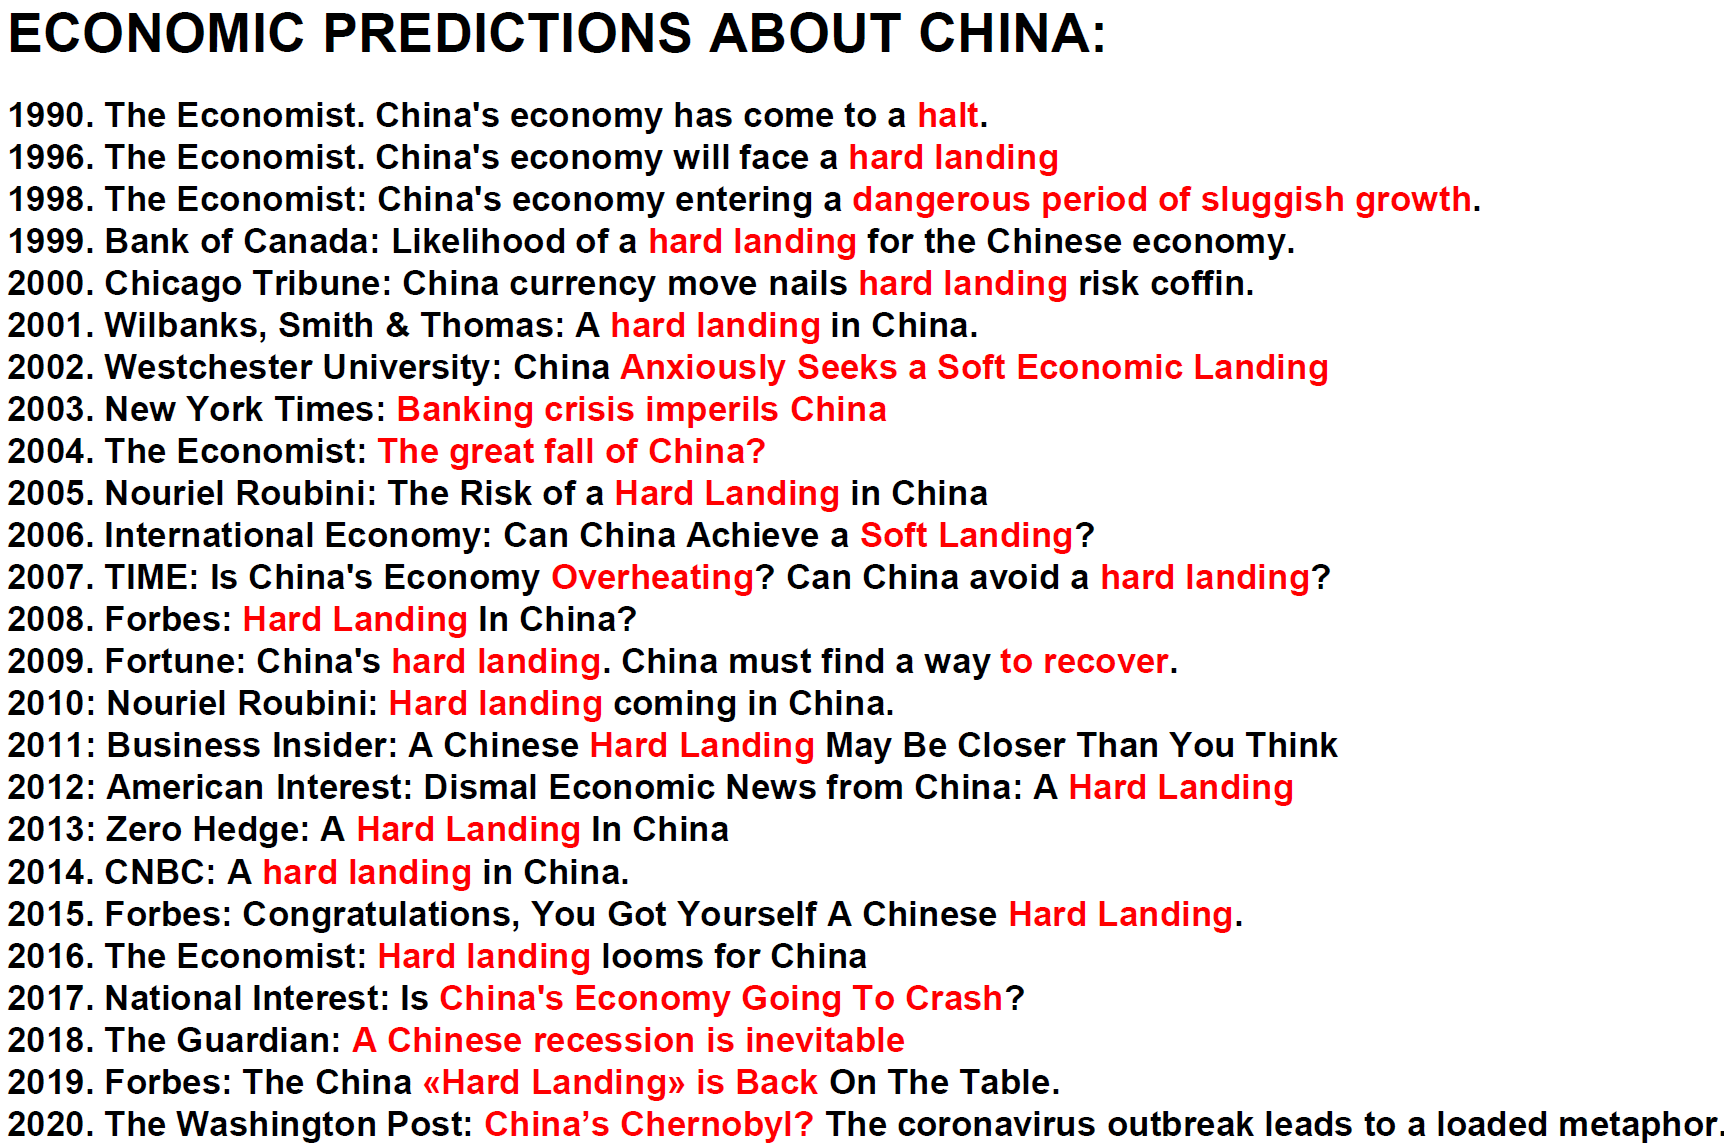
\includegraphics[width=0.8\textwidth]{Pictures/China_economic_prediction.png}
\end{figure}

\begin{itemize}
    \item GDP rose from $367.9$ billion yuan in 1978 to 99.1 trillion yuan
        (\$14.4 trillion) in 2019.
    \item Since 2010, China surpassed Japan and has become the second-largest
        economy in the world, accounting for around 16 percent of world economy
        in 2019 (30\% of world's economy growth), up 14 percentage points from
        1978.
    \item In 2013, China's GDP in purchasing power parity (PPP) terms overtook
        the USA's in 2013, and now accounts for nearly 19\% of global economy
    \item Per-capita GDP rose from 385 yuan (\$229) in 1978 to 70892 (\$10276)
        in 2019, lifting China from the notch of world's low-income to
        middle-income countries.
\end{itemize}

\paragraph{The government favors hardware over software}

Behind the hard line towards internet companies is a rethinking of which
sectors really matter for national progess. China's government is now convinced
that manufacturing matters more. Unlike the US, China does not see its internet
companies as leaders of national innovation, but as sources of social problems.
Internet entrepreneurs will get even more generous subsidies.

\vspace{1\baselineskip}

The current regulatory shift therefore is not negative for all Chinese listed
companies, or even all technology companies. Policy support for strategically
important sectors is ramping up, but most of those are hardware rather than
software: most prominently, semiconductors and renewable energy. Hardware
tech companies stock prices have done better than those of international
platforms in recent weeks, which could be the start of a trend.

\vspace{1\baselineskip}

In 1981, three years after Deng's reform project was launched, almost 90\%
of chinese people lived in extreme poverty by the definition of the World
Bank (\$1.9 per day). By 2016, that number had dropped to less than 0.5\%.
By the end of 2020, it is 0.

\vspace{1\baselineskip}

2016 the world's largest radio telescope with a folded aperture in China
was completed. The so-called FAST is a spherical radio telescope with a
diameter of 500 meters. It began its work in Guizhou Province.

\vspace{1\baselineskip}

In 2006, the Qinghai-Tibet Railway began oberations on the world's highest
railway line, at an average elevation around 4500m above sea level. Tanggula
railway station at 5068m is the world's highest railway station.

\vspace{1\baselineskip}

The third fastest supercomputer in the world as of Nov 2019. The Sunday
TaihuLight was the world's fastest supercomputer for two years, from June
2016 to June 2018, according to the TOP500 lists. The record was surpassed
in June 2018 by IBM's Summit.

\vspace{1\baselineskip}

\begin{itemize}
    \item With progress on urbanization and industrialization, more jobs
        were created in urban areas, from 2.6 million new jobs in 2000 to
        13.52 million in 2019.
    \item Total energy output rose from 627.7 million tons of standard coal
        in 1978 to 3.75 billion tons of standard coal in 2017.
    \item From 1978 to 2017, China's state revenue increased from 113.2 billion
        to 17 trillion yuan.
    \item China's retail sales of consumer goods grew from 155.9 billion yuan
        in 1978 to 41.16 trillion yuan in 2019.
    \item China's foreign trade volume rose from \$20.6 billion in 1978 to
        \$4.1 trillion in 2017. About 58.52\% of people lived in towns and
        cities in 2017, compared to 17.92\% back in 1978.
    \item China's high-speed railway developed from nothing. Up to 2017, the
        high-speed railway network covered 25000 km.
    \item Auto industry has witnessed an uptrend in production over the past
        40 years. The volume hit 29.02 million in 2017, up from 149000 back
        in 1978.
\end{itemize}

China has been one of the major driving forces in the world.

\vspace{1\baselineskip}

Chinese visitors account for a rising share of visitory and tourist spending
in many economies.

\vspace{1\baselineskip}

China is the world's anufacturing superpower.

\begin{itemize}
    \item China accounts for 30\% of global manufacturing output.
    \item Although it accounts for only 10\% of global houshold consumption,
        it was the source of 31\% of global houshold consumption growth from
        2010 to 2017.
    \item In many categories including automobiles, spirits, luxury goods,
        and mobile phones, China is the largest market in the world,
        accounting for about 30\% of global consumption.
    \item The world's second-largest source and second-largest recipient
        of FDI between 2015 and 2017.
\end{itemize}

China is so interconnected with other nations in trade that blocking china
as a trade partner would also cause effects for third countries.

\begin{figure}[H]
    \centering
    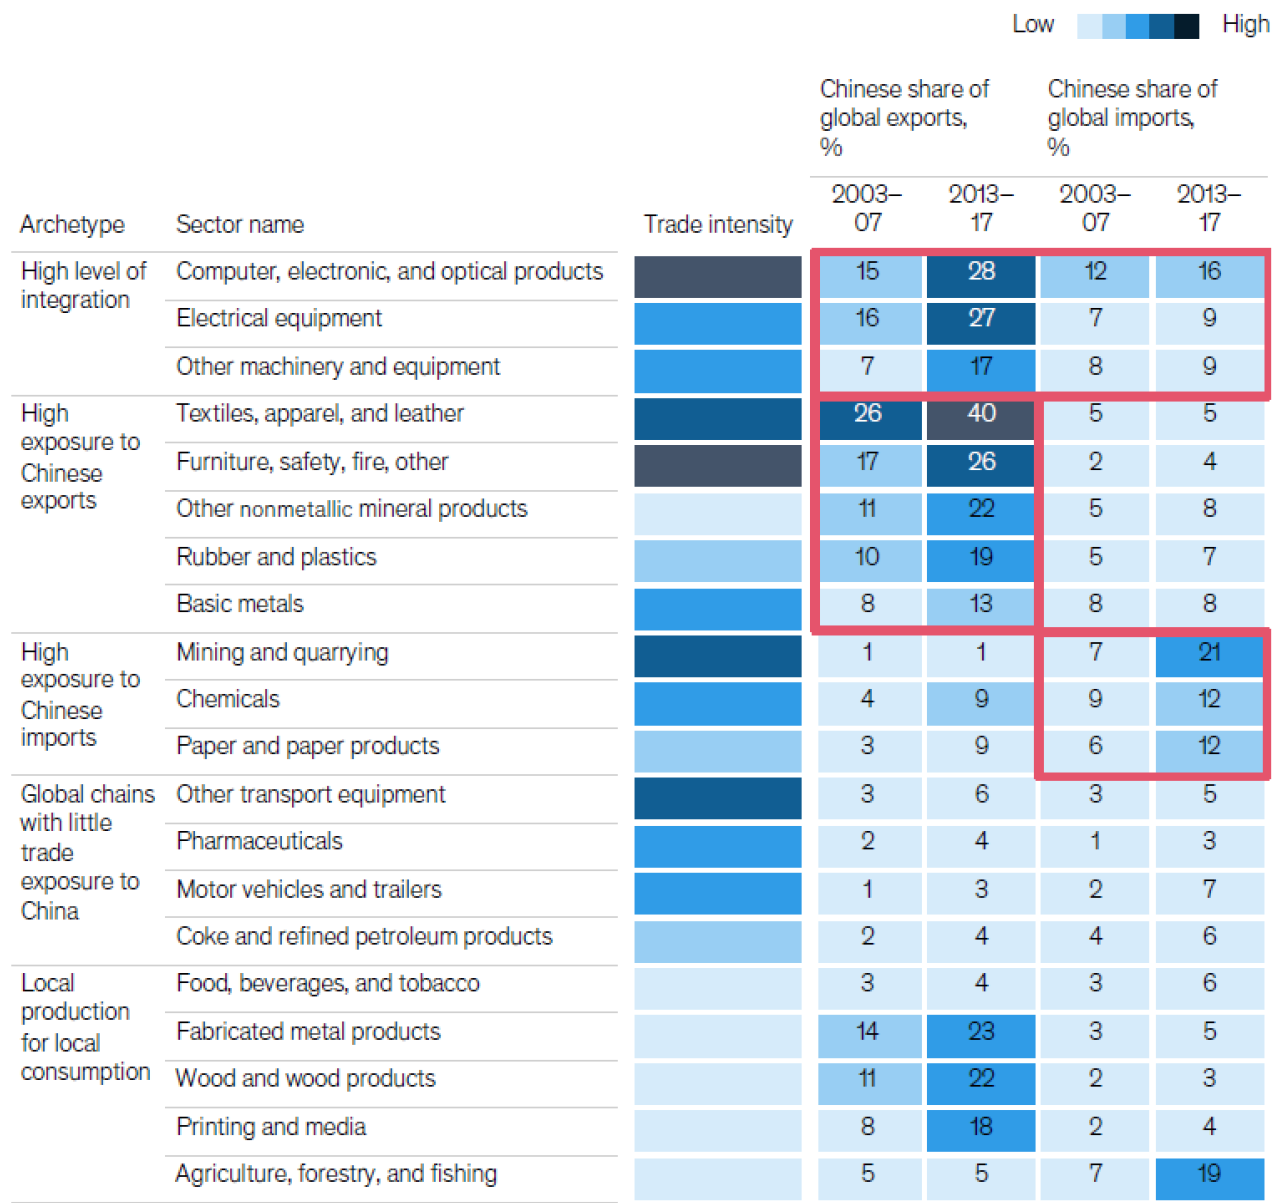
\includegraphics[width=0.75\textwidth]{Pictures/china_trade_1.png}
\end{figure}

\begin{figure}[H]
    \centering
    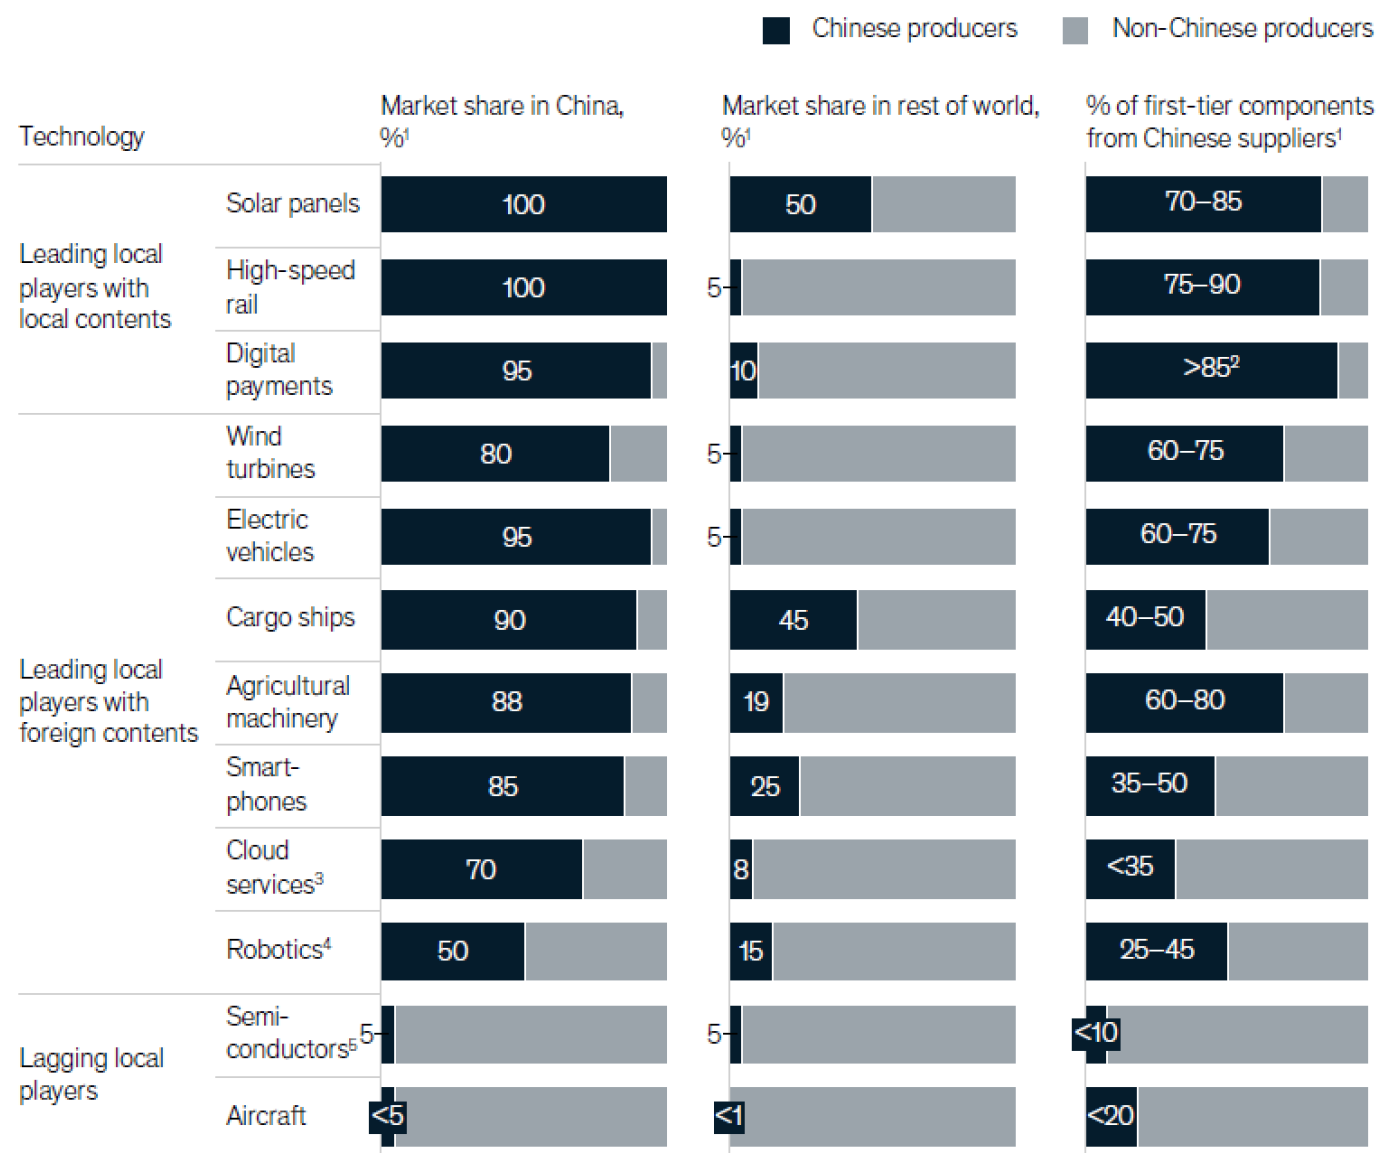
\includegraphics[width=0.7\textwidth]{Pictures/china_trade_2.png}
\end{figure}

\begin{figure}[H]
    \centering
    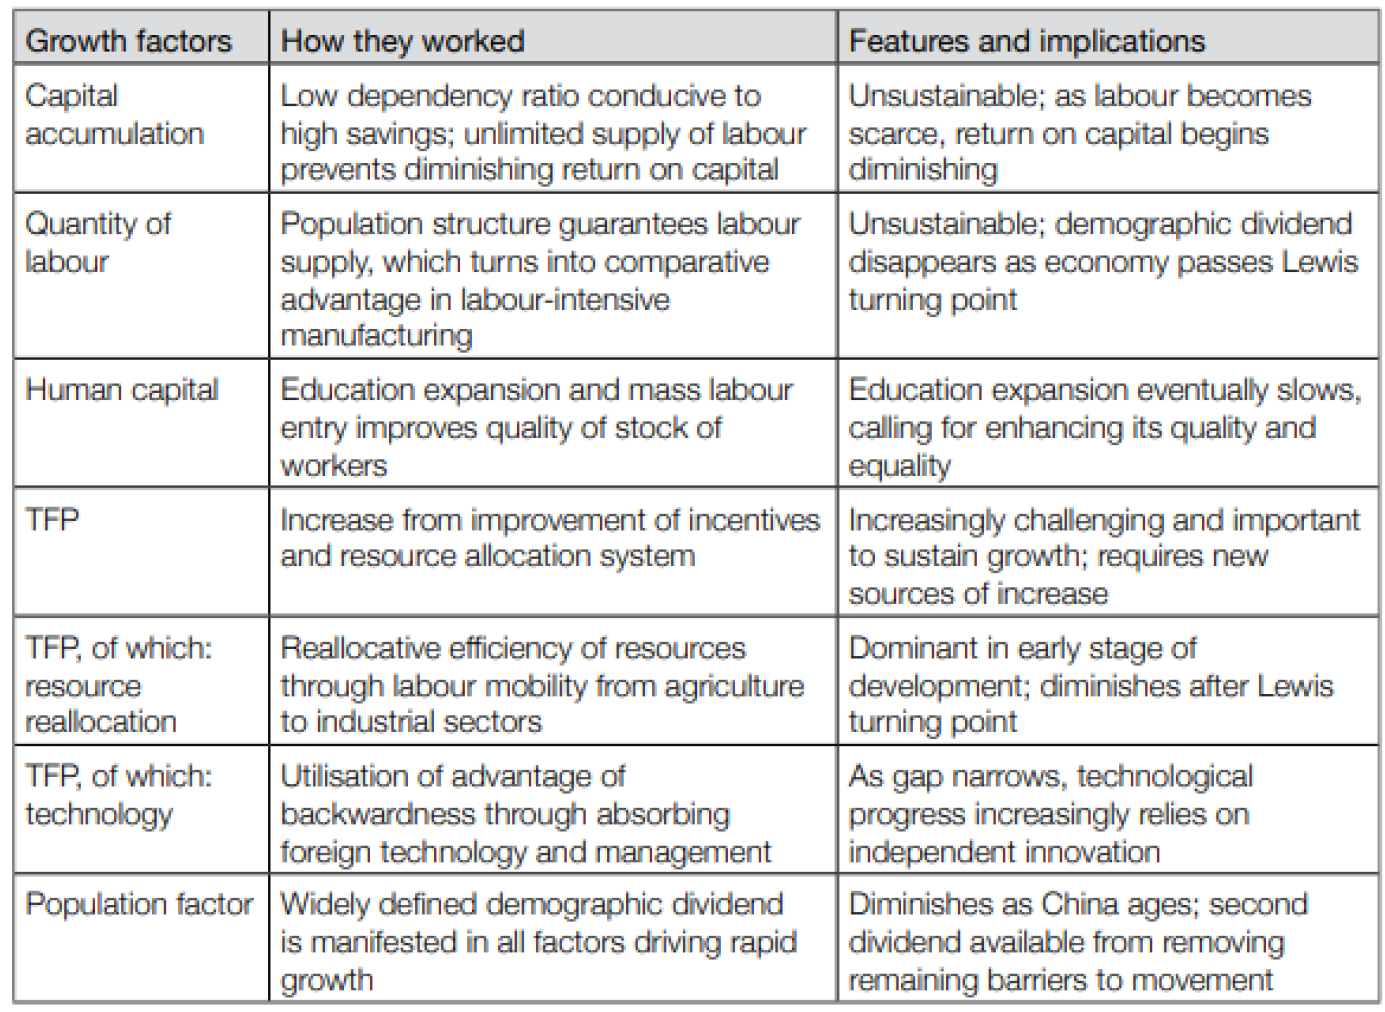
\includegraphics[width=0.8\textwidth]{Pictures/china_trade_summary.png}
    \caption{Summary Chinese Trade}
\end{figure}

\subsection{China is an old superpower with a recent brief dent (How China fell
and woke up)}

History of China: Ancient China and Century of Humiliation (1839-1949).
People's Republic of China: 1949-1978 and 1979-now.

\begin{figure}[H]
    \centering
    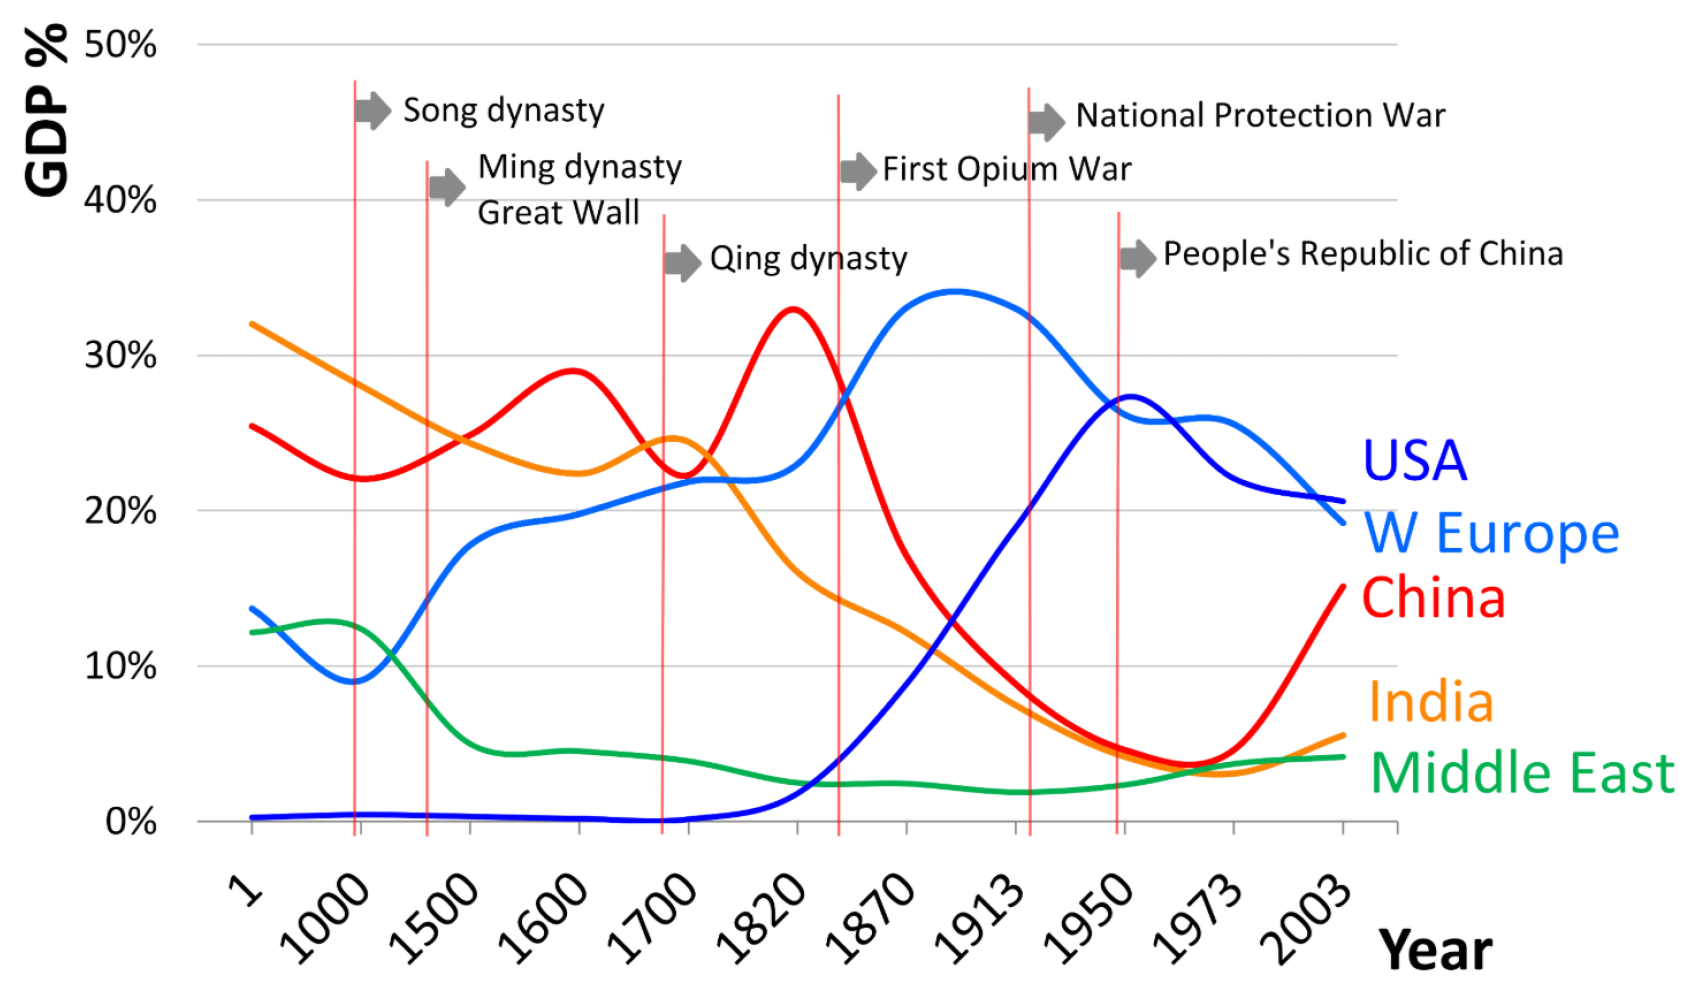
\includegraphics[width=0.8\textwidth]{Pictures/GDP_time_china.png}
\end{figure}

The european explorer Marco Polo (1254-1324 CE) traveled on the trading routes
centered on the Silk Road and described them in depth in his famous work but
he is not credited with naming them. Both terms for this network of roads were
coined by the German geographer and traveler, Ferdinand von Richthofen, in
1877 CE, who designated them 'Seidenstrasse' (silk road) or 'Seidenstrassen'
(sild routes). Polo, and later von Richthofen, make mention of the goods which
were transported back and forth on the Silk Road.

\paragraph{Four great inventions}

\subparagraph{Paper Making}
In the early Western Han Dynasty, China invented papermaking.
Papermaking is a great revolution in writing materials.

\subparagraph{Printing}
In the early Tang Dynasta, engraving printing was invented from the
seals and engraving stone.

\subparagraph{Movable type printing}
In the early 11th century, Bi Sheng, a civilian in the Northern Song Dynasty,
invented movable type printing, which was more than four centuries earlier
than the European invention. The spread of North Korea and Japan to Egypt and
Europe to the west. The invention of printing is a major contribution to the
spread and preservation of human culture.

\subparagraph{Gunpowder}
It was invented by ancient alchemists in China, and the books in the middle
of Tang recorded the method of making gunpowder. It was used in the military
in the late Tang Dynasty. It was invented in the Southern Song Dynasty, and
was introduced into Arabia and Europe in the 13th century. The invention and
spread of gunpowder changed the medieval mode of warfare and was a major
event in the military era.

\subparagraph{Compass}
During the Warring States period, people made the instrument "Sinan" indicating
the direction, and later using the principle of magnet guide to make a compass.
In the Song Dynasty, the magnetized steel needle support was fixed in an
azimuth-engraved disk for pointing. This is the compas, also known as the
compas needle. The compass of the Northern Song Dynasty was used for navigation.
Introduced to Arabia and Europe in the 13th century. The invention and spread
of the 13th century. The invention and spread of the compass privided important
conditions for european navigators to explore new routes.

\subsubsection{Century of Humiliation (1839-1949)}

In this period, China suffered major international fragmentation, lost almost
all of the wars it fought, and was often forced to give major concessions to
the great powers in the subsequent treaties. In many cases, China was forced
to pay large amounts of reparations, open up ports for trade, lease or cede
territories and make various other concessions of sovereignty to foreign
"spheres of influence", following military defeats.

\begin{itemize}
    \item Defeat in the First Opium War (1839-1842) by the UK.
        \begin{itemize}
            \item Treaty of Nanking (Aug 1942): cession of Hong Kong; four
                additional "treaty ports" opened for foreign trade; 21 million
                dollars reparations (annual income 57 mio)
        \end{itemize}
    \item The Taiping Rebellion (1850-1864): One of the bloodiest wars in
        human history, the bloodiest civil war, and the largest conflict of
        the 19th century. Estimates of the war dead range from 10-30 million.
    \item Defeat in the Second Opium War (1856-1860) and the sacking of the
        Old Summer Palace by British and French forces.
    \item The Sino-French War (1884-1885)
    \item Defeat in the First Sino-Japanese War (1894-1895) by Japan
        \begin{itemize}
            \item Treaty of Shimonoseki (Apr 1895): recognized the indeppendence
                of Korea and renounced any claims to that country; ceded the
                Liaodong Peninsula, and the islands of Formosa (Taiwan) and
                Penghu (also known as Pescadores) to Japan; paid Japan a war
                indemnity of 200 million Kuping taels silver (7500 tonns),
                payable over seven years; opening of various ports and rivers to
                japanese trade.
        \end{itemize}
    \item The Eight-Nation Alliance (Austria-Hungary, France, Germany, Italy,
        Japan, Russia, the US and the UK) suppressing the Boxer uprising (1899-1901)
        \begin{itemize}
            \item Boxer Protocol (Sep 1901): 450 million taels of fine silver
                were to be paid as indemnity over 39 years to the eight naitons
                involved; to prohibit the importation of arms and ammunation; the
                destruction of Taku Forts; Legatin Quarters occupied by the
                Power shall be considered as a special area reserved for their
                use under exclusive control, in which Chinese shall not have the
                right to reside, and which may be defensible; concede the right
                to the Powers to station troops in 12 cities/places; Boxer and
                Governments or their nationals.
        \end{itemize}
    \item British expedition to Tibet (1903-1904)
    \item The Twenty-One Demands (1915) by Japan
    \item Japanese invasion of Manchuria (1931-1932)
    \item The Second Sino-Japanese War (1937-1945): 15-22 million death
\end{itemize}


The Moa Era (1949-1977): Mao Zedong's tenure as Chairman of the PRC triggered
sweeping changes for the country.

\begin{itemize}
    \item 1953-1957: First 5-Year Plan: The program's aim was to boost
        China's industrialization. Steel production grew four-fold in four
        years, from 1.3 million tonnes to 5.2 million tonnes. Agriculture
        output also rose, but it couldn't keep pace with industrial production.
    \item 1958-1962: Great Leap Forward: The campaign emphasized China's
        agrarian-to-industrial transformation, via a communal farming system.
        However, the plan failed - causing an economic breakdown and the deaths
        of tens of millions in the great Chinese Famine.
    \item 1959-1962: Lushan Conference and 7000 Cadres meeting:
        Top leaders in the Chinese Communists Party (CCP) met to create
        detailed policy frameworks for the PRC's future.
    \item 1966-1976: Great Proletarian Cultureal Revolution:
        Mao Zedong attempted to regain power and support after the failures
        of the Great Leap forward. However, this was anoter plan that backfired,
        causing more deaths by violence and again crippling the Chinese economy.
    \item 1971: Joined the UN: The PRC replaced the ROC (Taiwan) as a permanent
        member of the UN. This addition also made it one of only five members
        of the UN Security Council - including the UK, the U.S., France, and
        Russia.
    \item 1972: President Nixon's visit: After 25 years of radio silence,
        Richard Nixon was the first sitting US President to step foot into the
        PRC. This helped re-establish diplomatic relations between the two nations.
    \item 1976-1977: Mao Zedong Death, and "Two Whatevers": After Mao Zedong's
        passing, the interim government promised to "resolutely uphold whatever
        policy decisions Chairman Mao made, and unswervingly follow whatever
        instructions Chairman Mao gave."
    \item 1979: "One-Child Policy": The government enacted an aggressive
        birth-planning program to control the size of country's population,
        which it viewed as growing too fast.
    \item When the PRC (People's Republic of China) was established in
        1949, China accounted for 4.2\% of the global economy, but this
        number increased to only 4.9\% by 1978. In 1949, GDP per capita was
        \$23, and was \$156.4 in 1968.
\end{itemize}

Before 1978 the leaders were more ideologistic. After, no matter which
regime, as long as it works.

\paragraph{Reform and development strategy}
Justin Yifu Lin and Zhongkai Shen (2018). In China's 40 Years of Reform and
Development 1978-2018.
\begin{itemize}
    \item Why was China able to achieve such extraordinary growth during
        its transition? Why was China able to grow so dynamically during the
        reform period? Answer: The latecomer advantage.
    \item Why was China unable to attain similar success before its
        transition started? If the latecomer advantage was the reason
        for China's extraordinary growth performance after 1978, the same
        advantage should have existed for centuries before 1978, so why did
        China not benefit before the reform and opening-up? Answer: Because
        China voluntarily gave up the latecomer advantage.
    \item Why did few other transitional economies perform equally well?
        Answer: Because other economies followed the wrong transition strategy:
        the neoliberal 'Washington consensus', which was based on the argument
        that the misallocation of resources caused by excessive government
        intervention led to unsatisfactory economic performance. 'shock therapy'.
        China adopted a pragmatic, gradual and dual-track approach.
\end{itemize}

\subsection{China is a Confucious dominant country (East and West culture difference)}

\begin{itemize}
    \item Shower: West: Morning, East: evening
    \item Waiting Queue: West: line, East: bunch of people
    \item Way of life: West: indipendence and individualism, East: community oriented
    \item Restaurant: West: calm, East: noisy
    \item Punctuality: West accurate, East: flexible
    \item Opinions: West: straight forward, East: complicated
    \item Making Contacts: West: linear relationships with few people, East: circular relationships across many people
    \item Anger/Displeasure: West: If unhappy, emotions can be perceived through body language etc,
        East: Norm is to hide displeasure
    \item View of Myself: West: most important, East: part of the sum.
    \item Handling Problems: West: most direct approach, East: involve indirect approach
    \item The Boss: West: weaker influence, East, great authority and influence as well as respect.
    \item Truth: West: honest, East: liar
    \item Talking about Money: West: no problem, East: not appropriate to talk about money
\end{itemize}

\subsubsection{Confucianism}
The main foundations of Confucianism emphasize duty, sincerity, loyalty,
honor, filial piety, respect for age and seniority. As individuals maintain
harmonious relations among themselves, society itself becomes stable.
\begin{itemize}
    \item Balance
    \item Hamony
    \item Modest
    \item Hierarchy
    \item Seniority
    \item Internal Hamony
\end{itemize}
Chinese business culture is largely influenced by Confucianism.
The Confucian concept of Guanxi means that a relationship network is crucial
and based on the values of solidarity, loyalty, modesty and courtesy.
Hierarchy in China, both in business and privacy, is purely vertical and highly
respected. Chinese people will be careful to save face in order to protect
individual reputations, influence and dignity. Some of these values have
slowed down over the last decade and modern Western business approaches are
gaining ground.

\paragraph{Collectivism vs. Individualism}
This is referred to as the degree to which individuals in a certain country
prefer acting as individuals rather than as members of groups. This dimension
focuses on the relationship between the individual and the larger social
groups.

It encourages people to pull up their socks and get out of poverty. On the
other hand, China as collectivistic society encourages more group work and
puts more emphasis on strong relationship between individuals hence the basis
of guanxi. To them, the needs of a group are way more important than
individual needs.

\paragraph{Characteristics of Individualistic Cultures}

\begin{itemize}
    \item Fosters contractual relationships that revolve around the basics
        of exchange. In such cultures, calculation of the profit or loss
        of engaging in a particular behaviour is calculated before going
        for it.
    \item Concentrates more on self and the very dear or near ones as well as
        concern with behavioural relationships as well as own interests, needs
        and own goals.
    \item More emphasis on personal pleasure, over duties, fun, enjoyment and
        social norms. They are part of in-groups, but they hardly have any
        influence on their lives.
    \item Value independence and self-sufficiency with self-interest placement
        rather than collective interests. In such societies, confrontation is
        an acceptable attribute.
    \item They hold unique beliefs and decisions are made based on individual
        needs.
\end{itemize}

\paragraph{Characteristics of Collectivistic Cultures}

\begin{itemize}
    \item For maintenance of social harmony among in-group members, the
        behaviour must subscribe to the social norms established.
    \item More giving up of personal interests and sharing of resources to
        facilitate the colllective interests.
    \item Before making any major decision must consider the implications to
        the wider collective.
    \item Favoritism expecially to in-groups including family and friends.
    \item Be a part of few influential in-groups and inclining towards
        conformality.
    \item Increased concern when it comes to ingroup members but show indifference
        or hostility towards out-group members.
    \item Much emphasis on hierarchy and harmony within the group.
    \item There are group norms which help in the regulation of behaviour.
\end{itemize}

\paragraph{FACE}
\begin{itemize}
    \item One of the central concepts in Chinese social life is 'face' (mianzi)
        because China is a collectivistic society in which social harmony is of
        utmost importance.
    \item Face reflects one's social self-esteem and the way one is regarded in
        society and interpersonal interactions.
    \item People can 'have face' as long as they are respected by others, but
        they can 'lose face' when they experience a public embarrassment.
    \item Public disagreement is a face-losing act of the Chinese: they prefer
        articulating the intentions in an indirect manner and leaving room for
        negotiations in private. Enhancing or saving others' face helps
        tremendously in building friendships and creating interpersonal goodwill.
    \item Face-saving actions sometimes are the cost of precision, accuracy, and
        clarity and may become compatible with honest or truthful communication
        practices.
\end{itemize}

\paragraph{Communication}

\begin{itemize}
    \item To Westerners, the word 'yes' suggests agreement and affirmation, but
        to Chinese a 'yes' may only convey the meaning of 'I am listening' with
        the purpose of showing attention and politeness.
    \item Chinese way of communication focuses on different elements, including
        implicit, context-based, listening-centered, and face-oriented mathods.
    \item Unlike the Western communication pattern, Chinese prefer to use an
        implicit language pattern - meaning is often implied of must be inferred.
    \item Also, they tend to take context and the specific situation into account
        when interpreting a word. So the ability to surmise and decipher hidden
        meanings is highly desirable in Chinese culture.
\end{itemize}

\paragraph{Modesty}

\begin{itemize}
    \item Chinese people value modesty and humbleness.
    \item To grow up as a Chinese, one learns not to take credit for one's
        behaviour or be boastful in any situation.
    \item Self-effacing/other-enhancing is common rule in Chinese socialization process.
    \item When receiving a compliment such as 'your son is an excellent boy',
        a Chinese would automatically say 'not really'.
    \item In Chinese culture, blatantly accepting a compliment is considered impolite.
    \item However, young Chinese professionals do not tend to keep a low profile.
        They tend to be more confident, self-expressive and direct.
\end{itemize}


\subsection{China in internally highly heterogenous and complex}

China often seems like a nonolith of 1.3 billion people, but it's not. It's
a mosaic of distinct regions, and understanding those regions is vital to
understanding China.

The Chinese are people with diverse physical traits, dialects and traditions.
They are multicultural, multireligious, and a multiethnic society, having
as many as 55 ethic groups as diverse and interesting as the geography and
the history of the country they inhabit. Several of them are descendant of
Arabs who came here via the Silk Road in early centuries.

\begin{itemize}
    \item Language: 8 main variants of spoken Chinese and hundreds of less common ones
    \item 56 Ethnicity
    \item Regional Stereotypes
    \item Economic development
\end{itemize}

\begin{figure}[H]
    \centering
    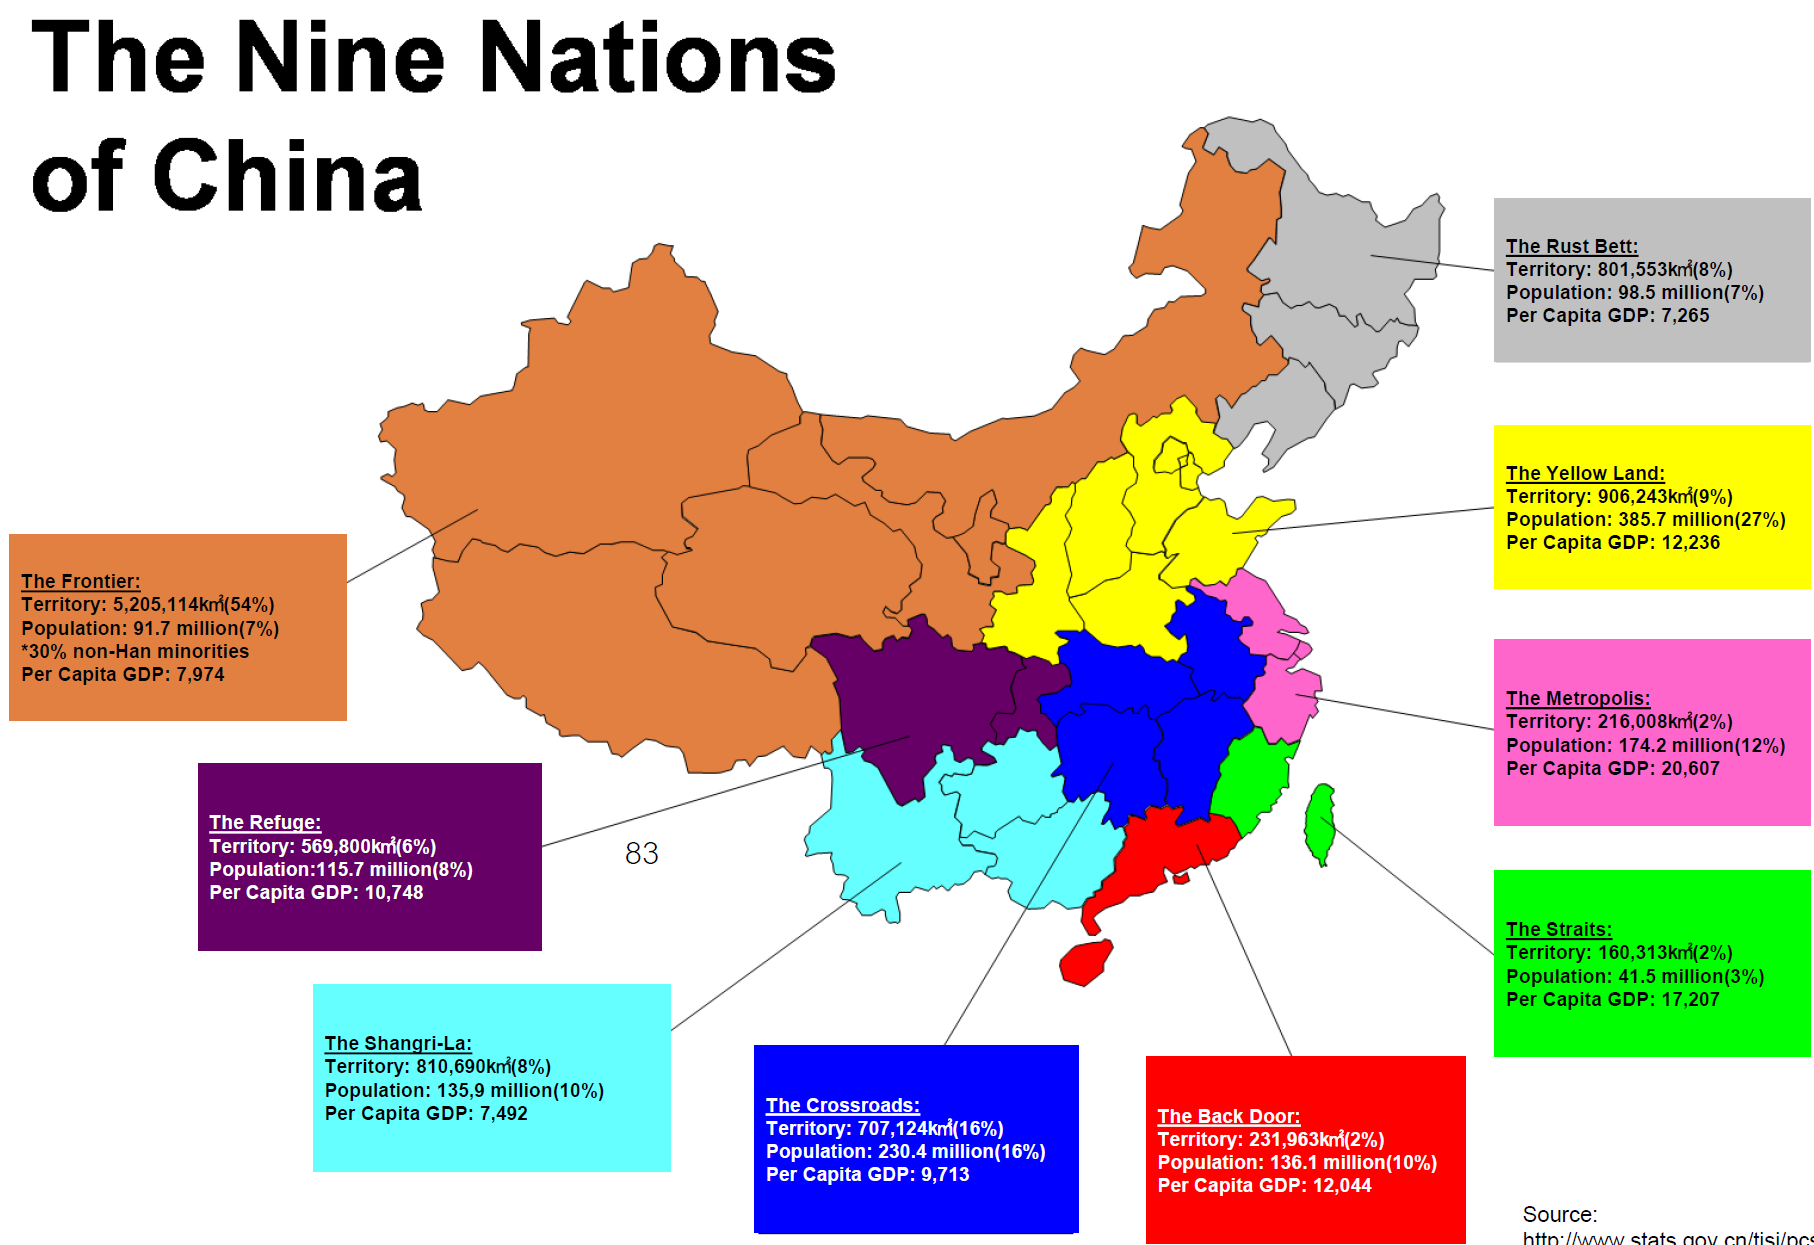
\includegraphics[width=0.9\textwidth]{Pictures/The_nine_nations_of_china.png}
    \caption{The nine nations of China}
\end{figure}

\begin{figure}[H]
    \centering
    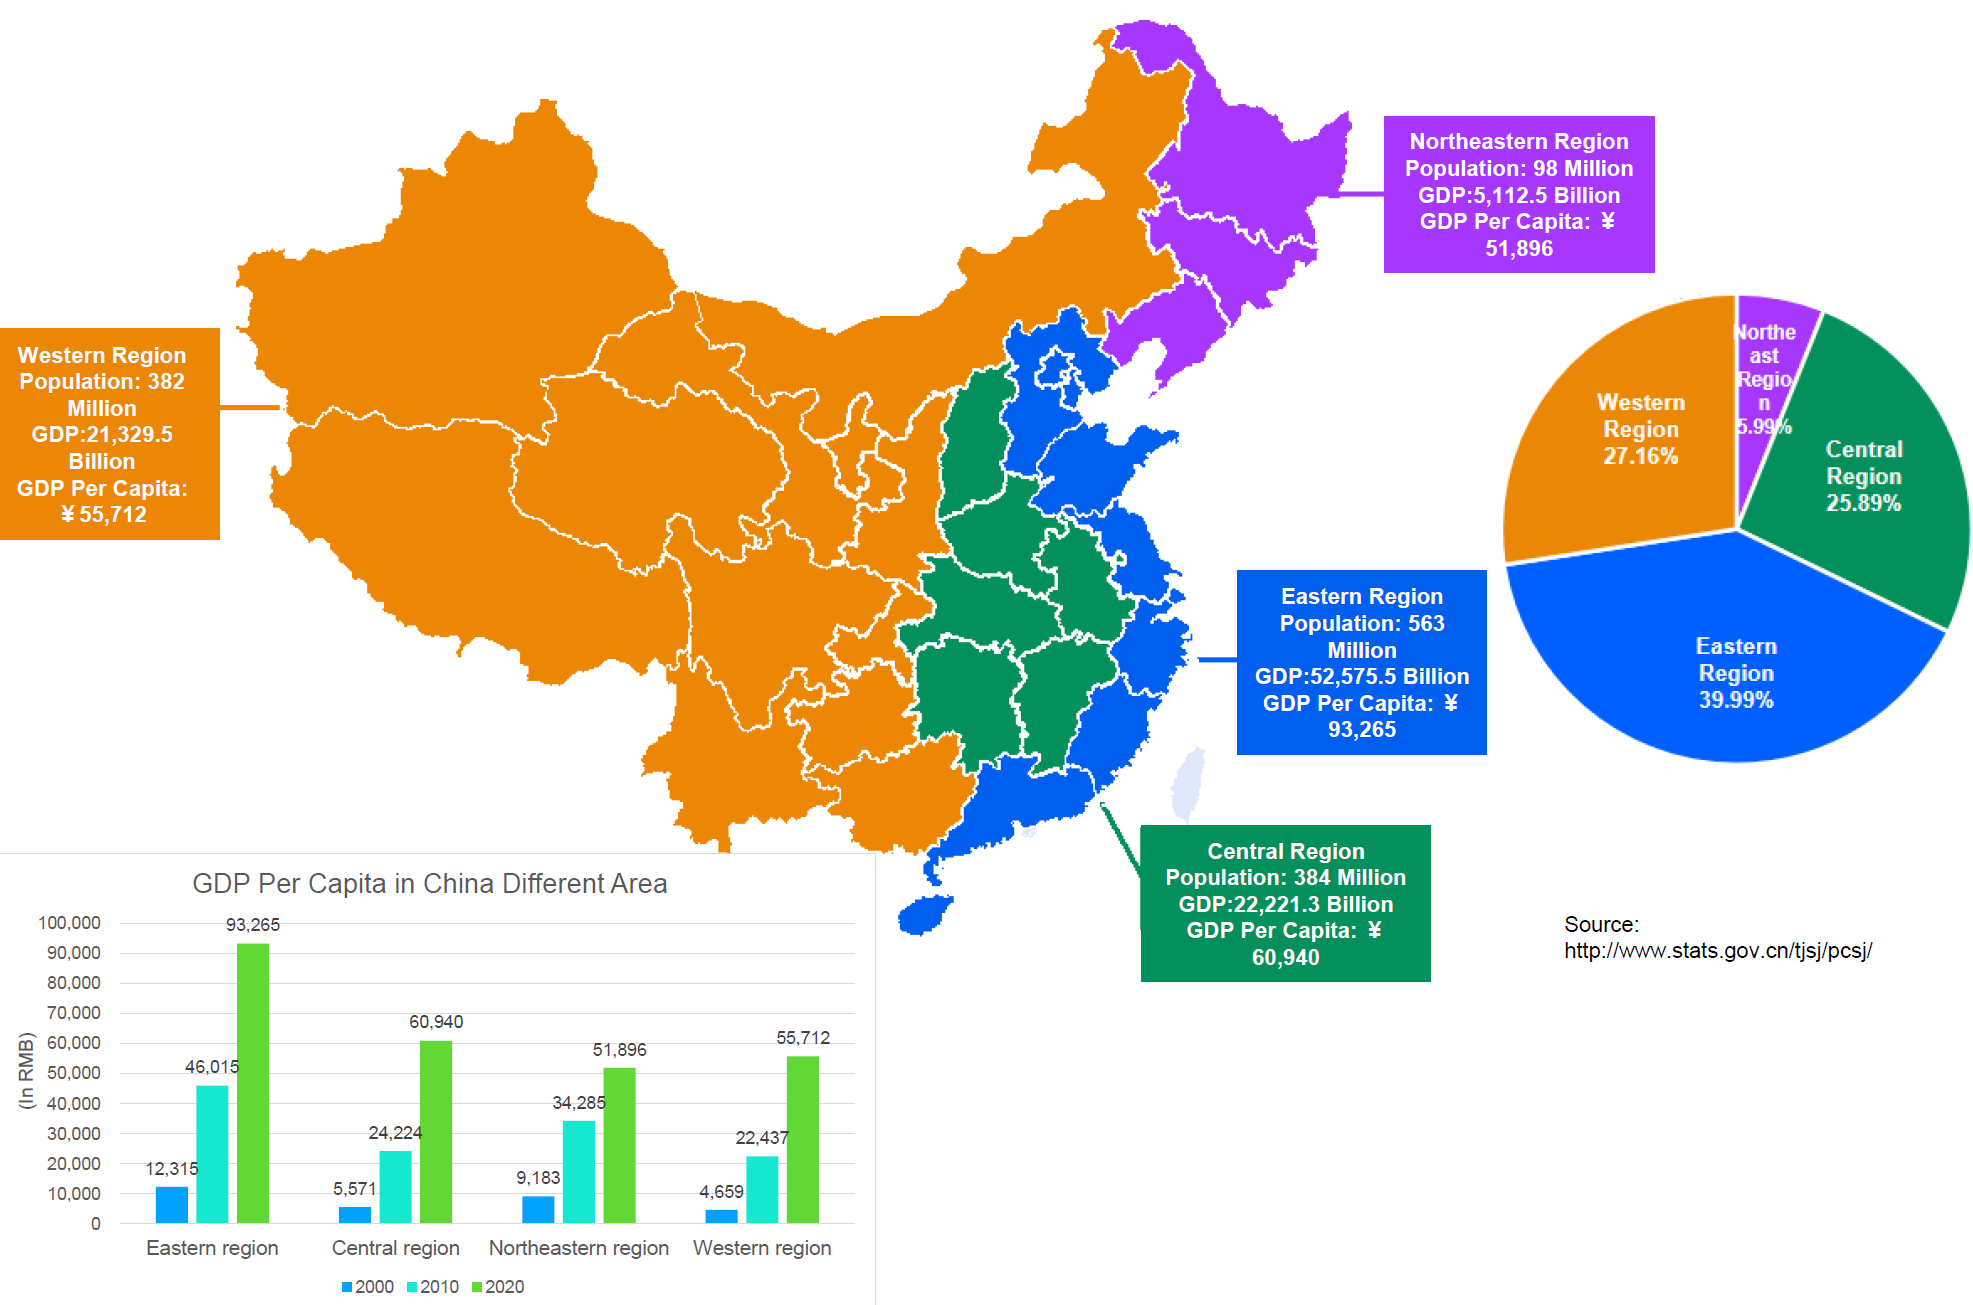
\includegraphics[width=\textwidth]{Pictures/The_nine_nations_of_china_2.png}
\end{figure}

There is a strong corrolation between political freedom and economic succes
of a country. Human societies must create stable sources of food energy, or
they die out. The ability to access saable sources of food energy is a function
of the available technology for growing, storing, and transporting food crops.
Given any particular state of technology, brute facts of nature determine the
amount of accessible food energy by affecting what can be grown, how much of it
can be grosn, whether it can be stored, and the distance at which it can be
traded.

\paragraph{4 Complex Adaptive Systems}

\begin{itemize}
    \item Transactional Complex Adaptive Systems
        \begin{itemize}
            \item Produce, relatively large fertile land, idiosyncratic weather shocks
            \item Shock $\Rightarrow$ move and trade $\Rightarrow$ rule of law and democratic system
        \end{itemize}
    \item Insurance Complex Adaptive Systems
        \begin{itemize}
            \item Produce, relatively large fertile land, aggregate weather shocks
                (massive shock lasting for years)
            \item Centralized coordination system
        \end{itemize}
    \item Subsistence Complex Adaptive Systems
        \begin{itemize}
            \item Produce but not be able to store (tropics with rainfall)
            \item No trade $\Rightarrow$ no surplus $\Rightarrow$ no investment
                in human capital and other infrastructural systems $\Rightarrow$ bands/tribes
        \end{itemize}
    \item Pastoral Complex Adaptive Systems
        \begin{itemize}
            \item Not possible to produce enough kilocalories $\Rightarrow$
                expand, move to outrun aggregate weather shocks (Steppe ecosystems)
        \end{itemize}
\end{itemize}


\pagebreak

\section{The collision of the two opposite mindsets: Innovation and Entrepreneurship
in China and Switzerland}

\subsection{Switzerland is an old friend of China}

Switzerland had significant economic interests in China at the time, especially
in Shanghai. The prompt recognition of the new communist government, as well
as Switzerland's status as a neutral country, allowed it to gain political
advantage and carve out a role as mediator in the region.

On October 7, 1949, the Federal Coucil (Swiss executive branch) had already
decided to recognise the Chinese government, in order to avoid being "either
one of the first or the last" to do so.

The official recognition came on January 17, 1950. Of the Western nations,
only Great Britain and Scandinavian countries were earlier in doing so.

The two countries formally established diplomatic relations on September
14 in the same year.

\vspace{1\baselineskip}

In the 1970s, the good Swiss-Chinese relations revolved mainly around the hope
that the Swiss economy might benefit from the future opening of the Chinese
market to external commerce. And indeed, in December 1974, Bern and Beijing
signed a trade deal - and then a free trade agreement 40 years later.

\begin{figure}[h]
    \centering
    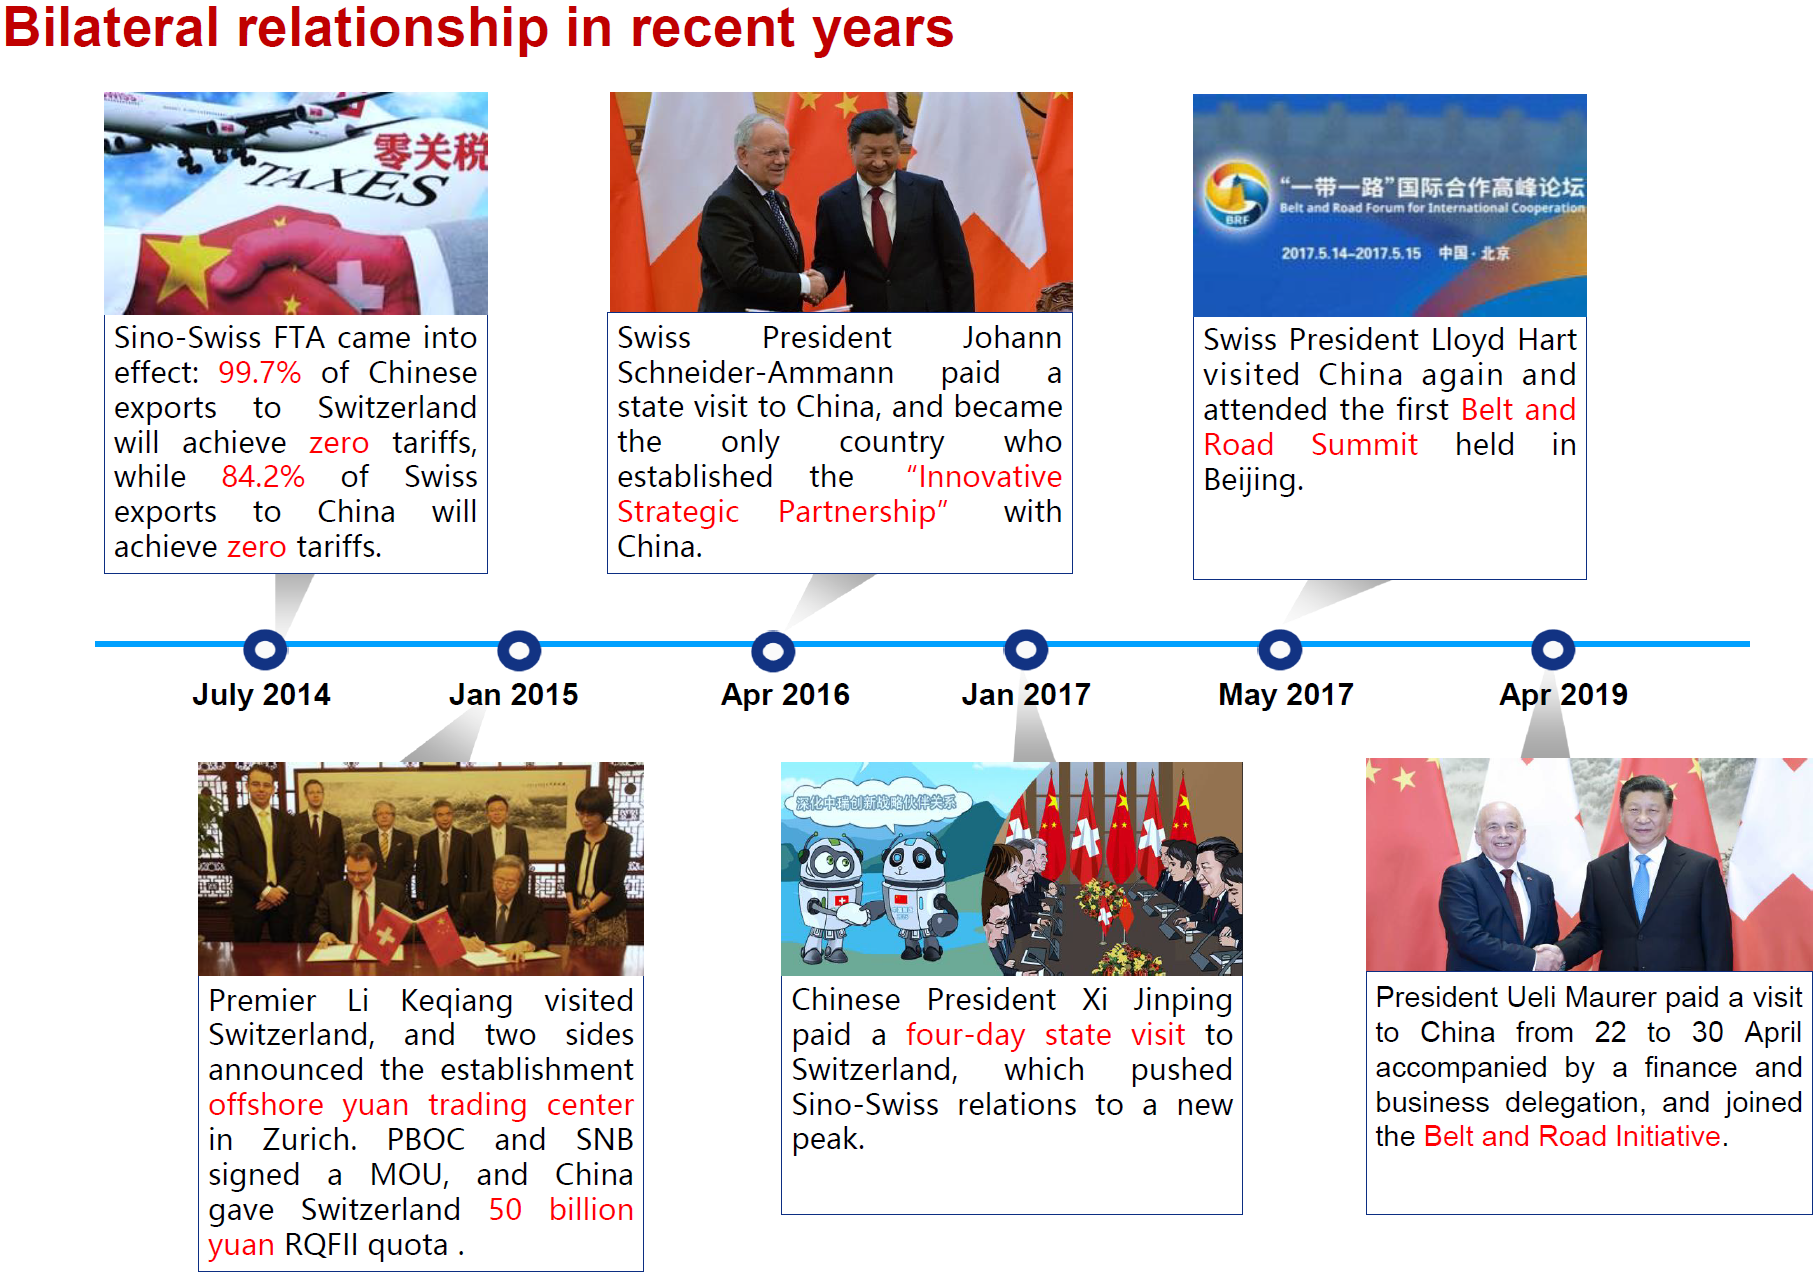
\includegraphics[width=0.8\textwidth]{Pictures/bilateral_china_switzerland.png}
\end{figure}

\begin{itemize}
    \item Switzerland has also strenghened financial ties with China over the
        years. In December 2018, UBS became the first foreign bank to gain
        majority control of a financial institution on mainland China by increasing
        its stake in the UBS Security joint venture to 51\%.
    \item In 2016, the China Construction Bank (CCB) became the first Chinese
        bank to open a branch on Swiss soil. CCB was followed by the Industrial
        and Commercial Bank of China a year later. The development has cemented
        Switzerland's positoin as a renminbi trading hub.
    \item A latent trade war currently exists between China and several Western
        countries, notably the US. Not with Switzerland though. Sino-Swiss
        economic ties were deepene by a free-trade agreement external link
        (FTA) that came into force on July 1, 2014. This is one of the few FTAs
        that China has signed external link with countries outside the
        Asia-Pacific region.
    \item Billed to save Swiss companies CHF 290 million annually by the time all
        trade barriers are lifted in 2023, a study last year found the FTA
        had achieved savings of CHF 100 million for both Swiss and Chinese
        firms in 2017.
    \item More than 80 Swiss companies are now in Chinese hands, with a total
        value of CHF 46 billion. The \$43.3-billion takeover of agrochemical
        giant Syngenta by the China National Chemical Corporation (ChemChina)
        in 2016 is the biggest acquisition ever by a Chinese company.
\end{itemize}

\paragraph{Import and Export:}

\begin{itemize}
    \item Export elasticity can be used to determine the effects of a sharp
        decline in China's growth on Swiss exports. Under the assumption of
        a constant exchange rate, export elasticity shows by how many
        percentage points the exchange growth in Switzerland would increase
        or decrease if the growth of China's GDP changes by one percentage
        point.
    \item The elasticity between Switzerland and China is not statistically
        significant. However, when you look at individual industries, you
        see that, at 2.6 percent points, the food industry in particular
        is very dependent on China's economic situation. The watch and
        machinery industries are also expecially sensitive to changes in
        the Chinese economy.
    \item Switzerland exports mainly finished products, so the Swiss economy
        is particularly dependent on Chinese final demand.
    \item Swiss exports to Germany are also influenced by China's economic
        development, as 20\% of exports to Germany are processed there and then
        exported to China, among other countries. One prominent example
        of this is the automotive industry.
\end{itemize}

\begin{figure}[H]
    \centering
    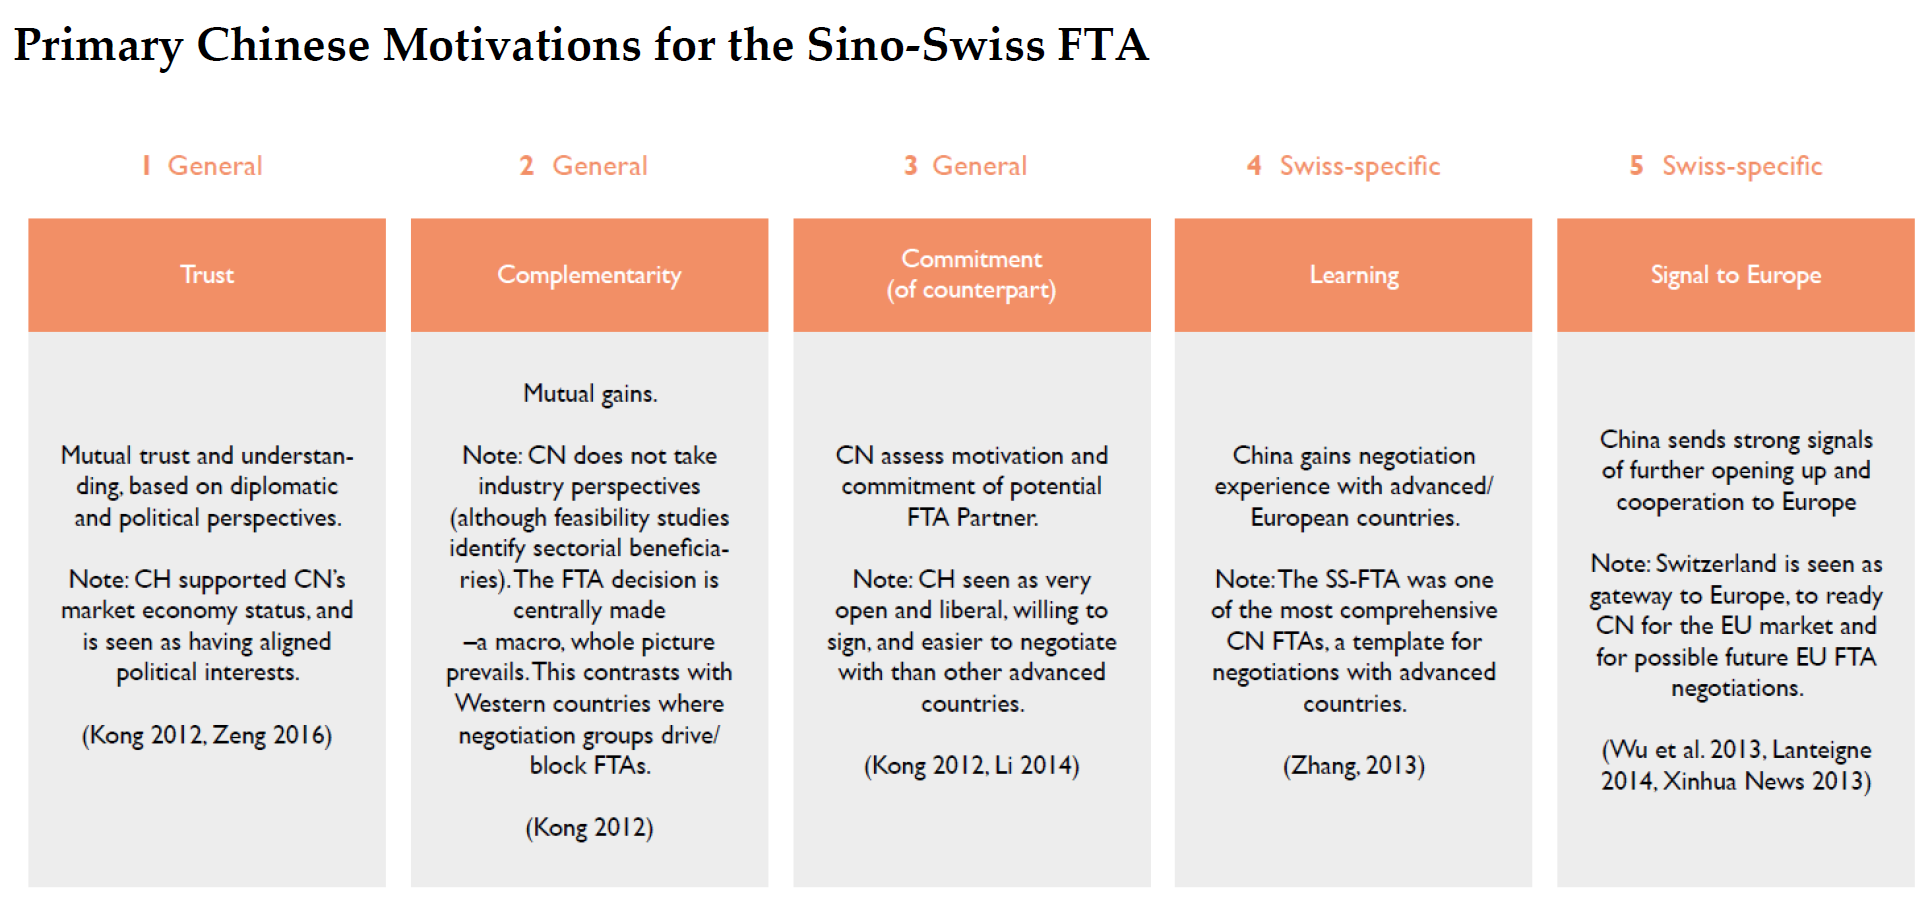
\includegraphics[width=0.9\textwidth]{Pictures/chinese_motivation.png}
\end{figure}

\begin{figure}[H]
    \centering
    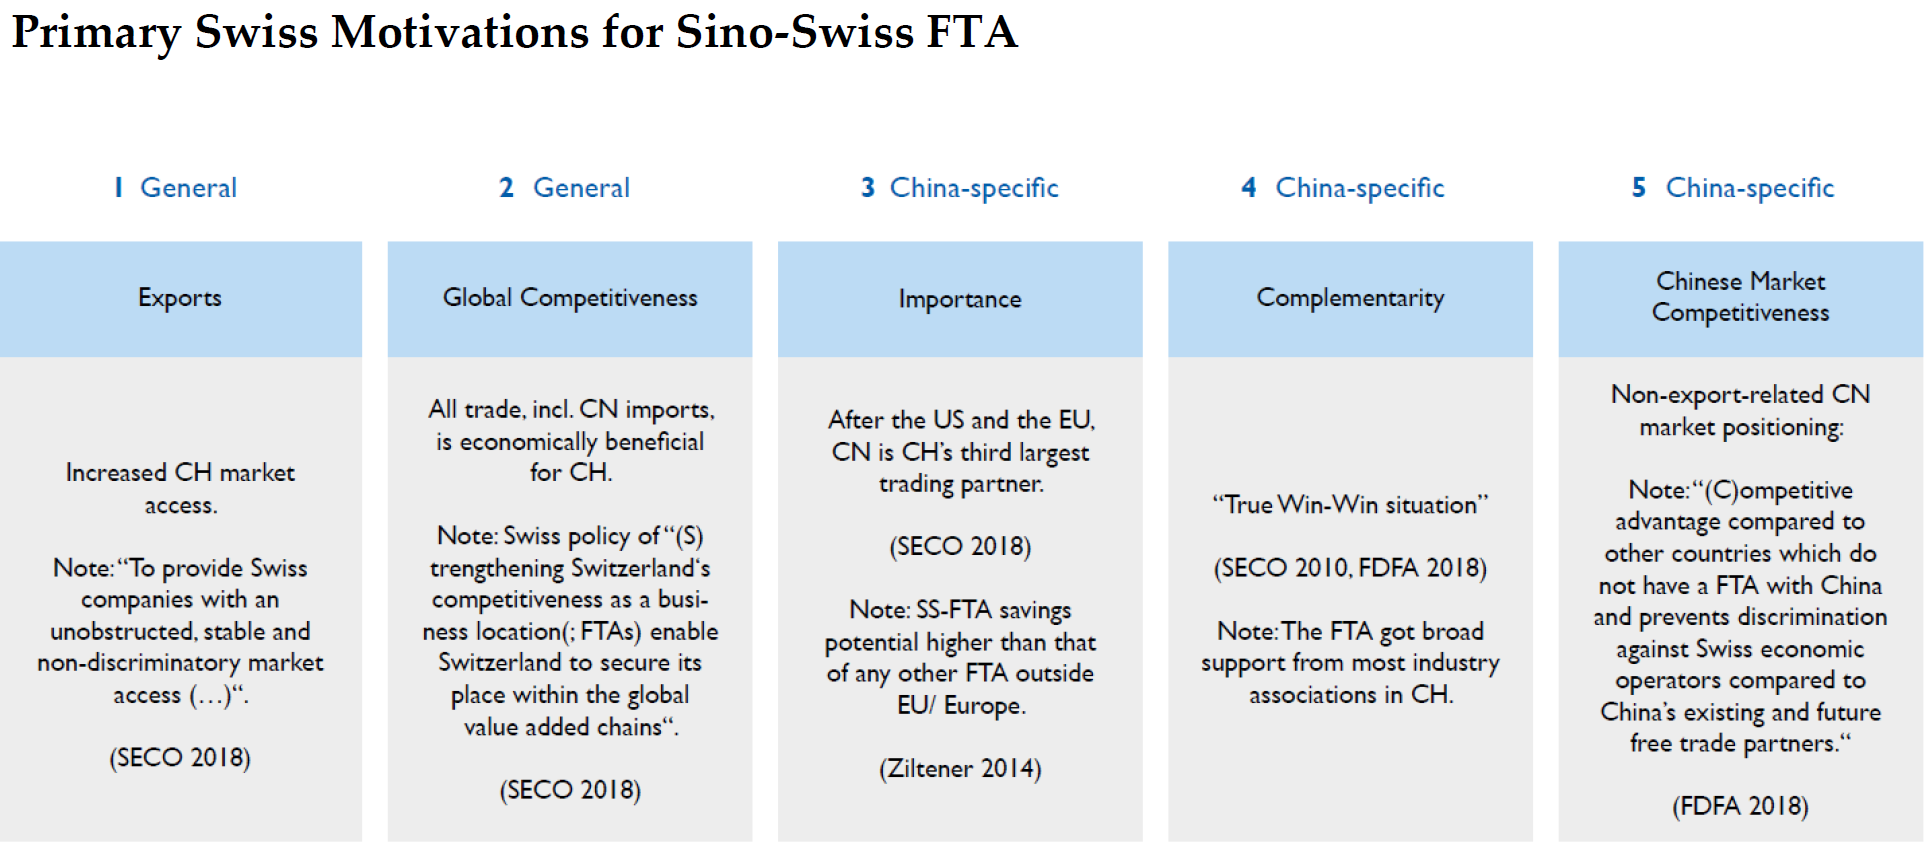
\includegraphics[width=0.9\textwidth]{Pictures/swiss_motivations.png}
\end{figure}


\paragraph{Why China needs Switzerland}

\begin{itemize}
    \item An entry point to European market
    \item A signal to Europe and the west advanced economies
    \item An entry point to the global stage via international organizations
    \item A neutral and friendly country
    \item A balance with Europe and the US
\end{itemize}


\paragraph{Why Switzerland needs China}

\begin{itemize}
    \item A huge and competitive market
    \item Engagement in an emerging power in the global stage
    \item A balance with Wurope and the US
    \item A "client" that Switzerland has been selling its neutrality service to
\end{itemize}

\paragraph{Chinese Strategy: three principle for cooperation}

China has been investing heavily in education, research and innovation for years
and shares a great deal of knowledge in fields including finance, science,
culture and environment protection. It is these areas especially that Switzerland
wishes to cooperate with the PRC, which is listed as a priority country in
Switzerland's Foreign Policy Strategy 2020-23. Three fundamental principles
underpin Switzerland's cooperation with China. These apply to bilateral relations,
multilateral cooperation and coordination in Switzerland.

\begin{itemize}
    \item Switzerland wishes to pursue an independent policy on China and defend
        its long-term interests and fundamental values. It will seek to do this
        through constructively critical dialogue wich Chinese representatves
        in the diverse areas of Swiss-China relations where there is an
        opportunity to engage on the issues.
    \item The Federal Council advocates the integration of China in the liberal
        international order and will seek to coordinate more closely with
        like-minded partners.
    \item Finally, it persues a balanced, coherent and coordinated approach
        to China that encourages exchanges with Parliament, the cantons,
        academia, the private sector and civil society
\end{itemize}

"Pioneering spirit and pragmatism, in addition to a strong stance in the
defence of Swiss interests and values, have moulded Switzerland's policy
on China for seventy years. They will continue to do so." - Ignazio Cassis


\subsection{Competence of the two nations}

\begin{figure}[H]
    \centering
    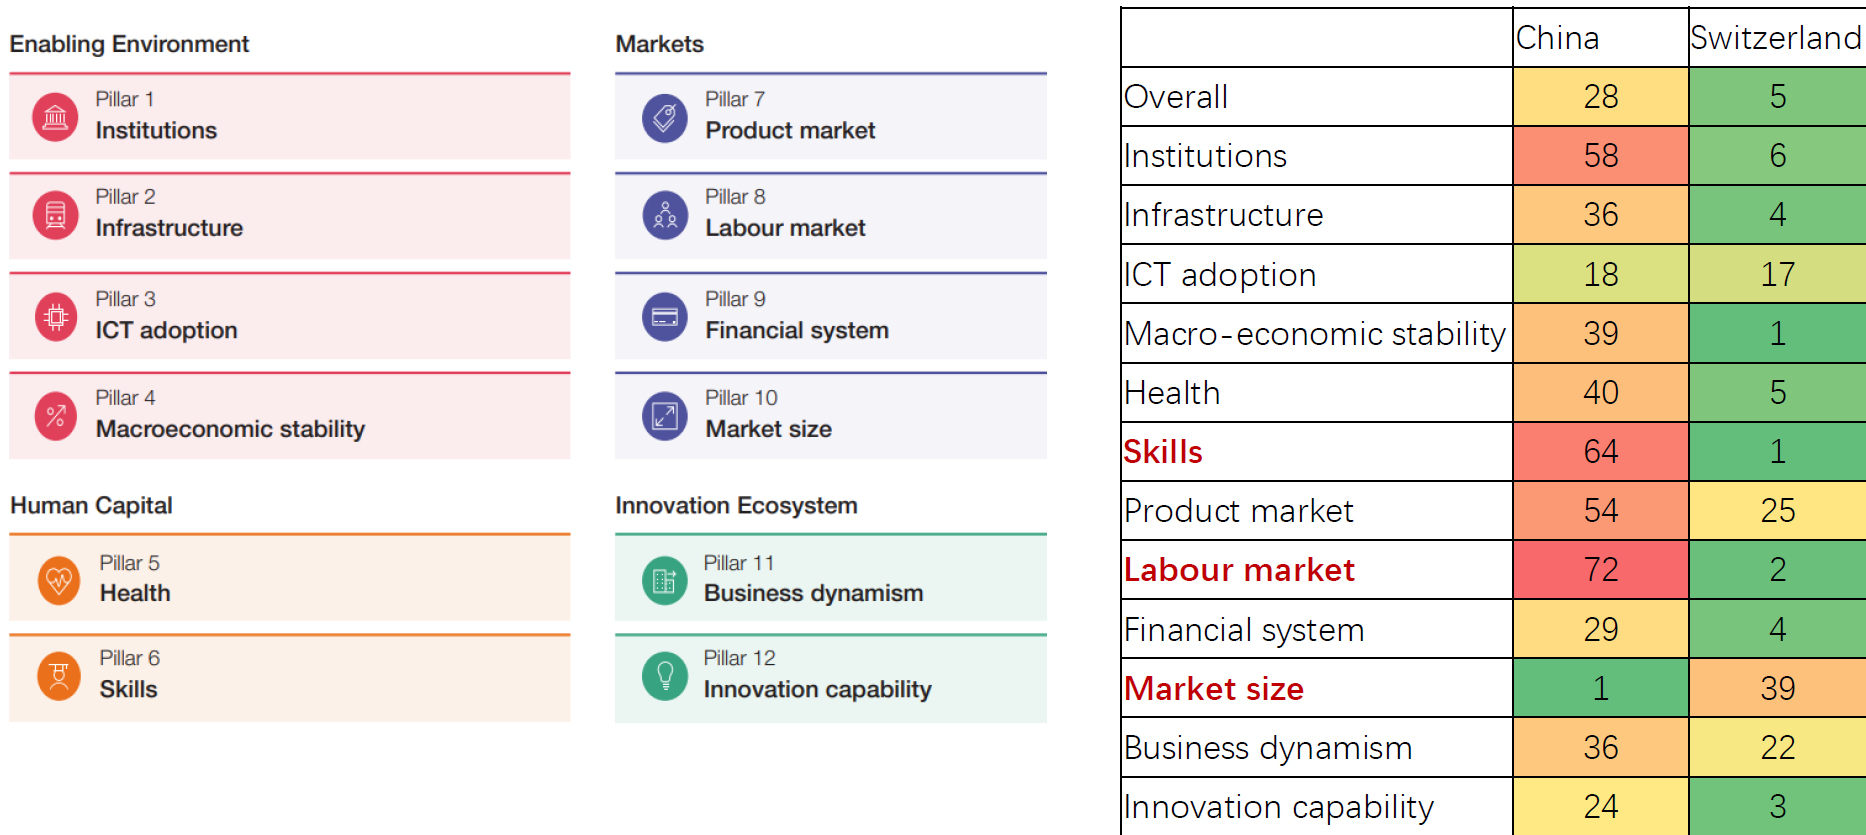
\includegraphics[width=0.9\textwidth]{Pictures/global_competitiveness_index.png}
    \caption{Global Competitiveness Index}
\end{figure}

\begin{figure}[H]
    \centering
    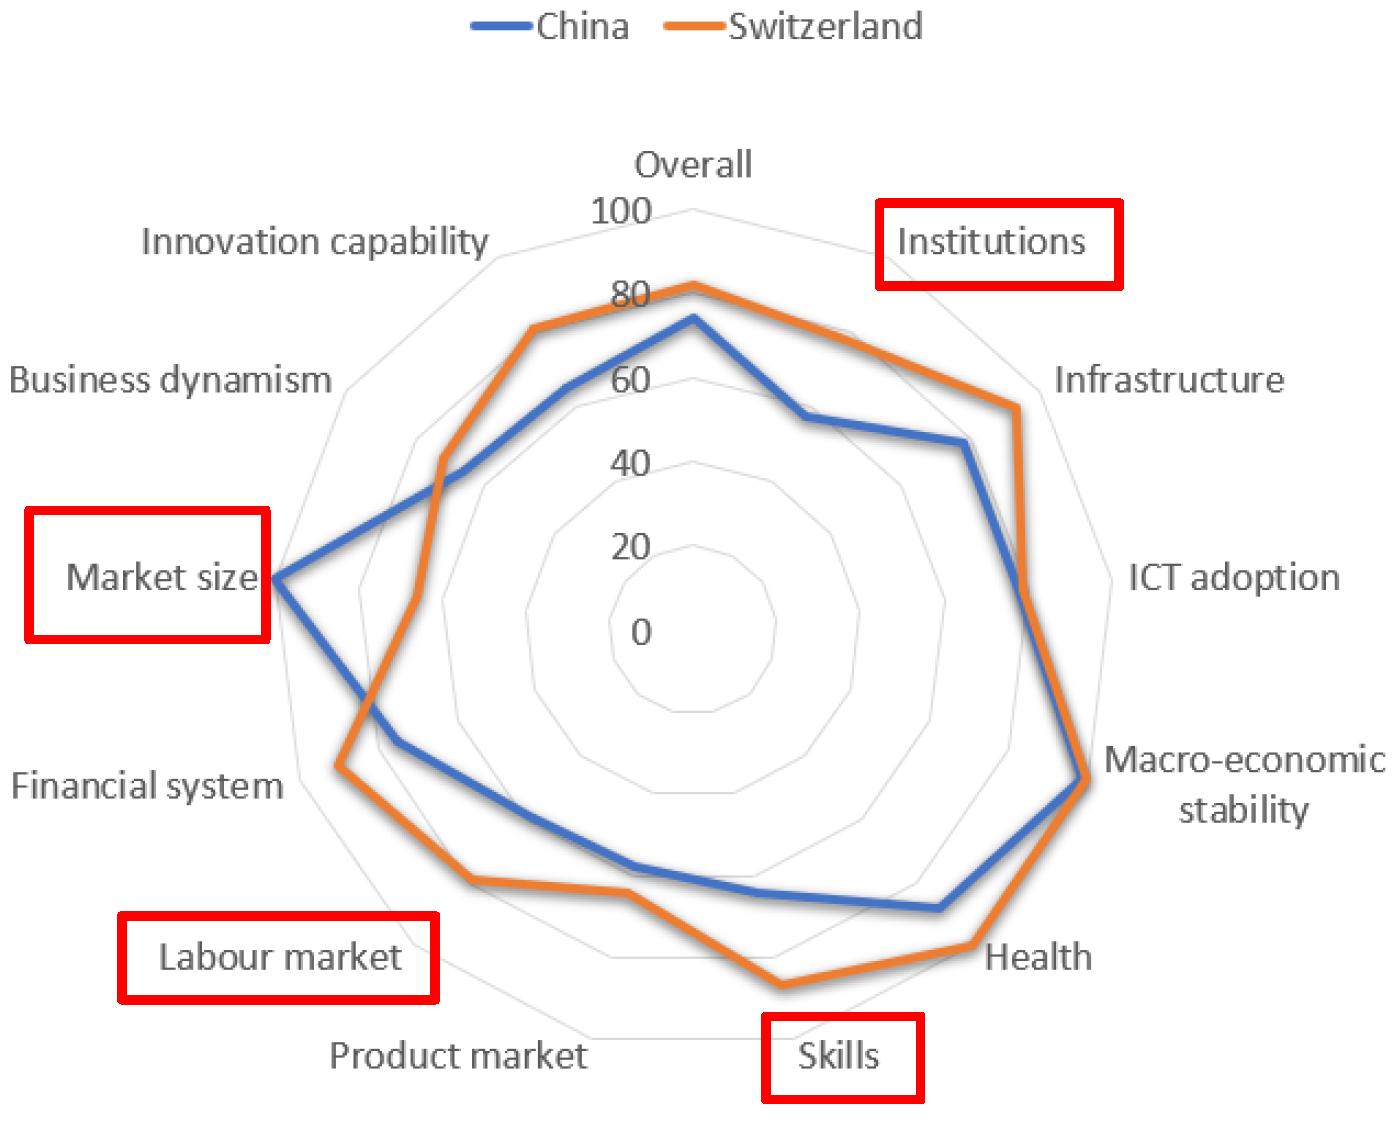
\includegraphics[width=0.5\textwidth]{Pictures/china_switzerland_wef.png}
\end{figure}

Switzerland has been innovation leader for the last 10 years.

\paragraph{Strengths}

\begin{itemize}
    \item G\uproman{2} strengths of China are found in six of the seven
        G\uproman{2} pillars, and mostly on the innovation output side
        of the G\uproman{2}, which captures countries' innovation results.
    \item Several of these strengths are in knowledge and technology outputs,
        the best ranked G\uproman{2} pillar for China. Here the country's
        strengths are sub-pillar knowledge creation and knowledge impact
        and indicators Patents by origin, Utility modely by origin, Labor
        productivity growth, and Hightech exports. In all of these indicators,
        China is world leader this year.
    \item In Creative outputs, China's strengths are sub-pillar Intengible
        assets and indicators Trademarks by origin, Industrial designs by
        origin, and Creative goods exports. In all of these areas, China ranks
        first in the world.
    \item On the innovation input side, China's strengths are found in four
        areas:
        \begin{itemize}
            \item In Human capital and research, an important G\uproman{2}
                strength is indicator Quality of universities, where China is
                placed 3rd worldwide, after the US and the UK.
            \item In Business sophistication, China's strength are indicators
                Firms offering formal training , R\&D financed by business,
                and Hightech imports.
            \item In Market sophistication, relative strengths are sub-pillar
                Trade, competition and market scale and indicator
                Domestic market scale, where China positions 1st globally.
            \item In Infrastructure, China's strength is indicator Gross capital
                formation.
        \end{itemize}
\end{itemize}

\paragraph{Weaknesses}

\begin{itemize}
    \item China's weaknesses in the G\uproman{2} are found in all G\uproman{2}
        pillars, except for knowledge and technology outputs.
    \item Most of these weaknesses are found on the innovation input side of
        the G\uproman{2}, which captures the investment that economies
        make to produce more and better innovations.
    \item In Institutions, China's weaknesses are sub-pillar Regulatory
        environment and its indicator Cost of redundancy dismissal.
    \item In Human capital and research, relative weaknesses are sup-pillar
        Tertiary education and indicator Tertiary inbound mobility.
    \item In Infrastructure, China presents relative weaknesses in two
        indicators within the area Ecological sustainability - GDP per unit
        of energy use and environmental performance.
    \item Indicator Microfinance gross loans in a relative G\uproman{2}
        weakness in Market sophistication.
    \item In Business sophistication, indicators R\&D financed by abroad
        and FDI inflows are G\uproman{2} weaknesses for China.
    \item Three relative weaknesses are found in Creative outputs in indicators
        National feature films, Printing and other media, and Wikipedia edits.
\end{itemize}

\subsection{Swiss startups and innovation}

471 ETH spin-offs since 1996 (93\% 5-Year survival ratio), 41 acquired or went IPO.

The ETH Domain under the Swiss Confederation, which includes 2 federal universities
and 4 federal institutions, forms the backbone of Swiss scientific and
technological innovation, incubating 60-100 Hightech companies each year, with
ETH Zürich being the largest institution in the domain.

\begin{figure}[h]
    \centering
    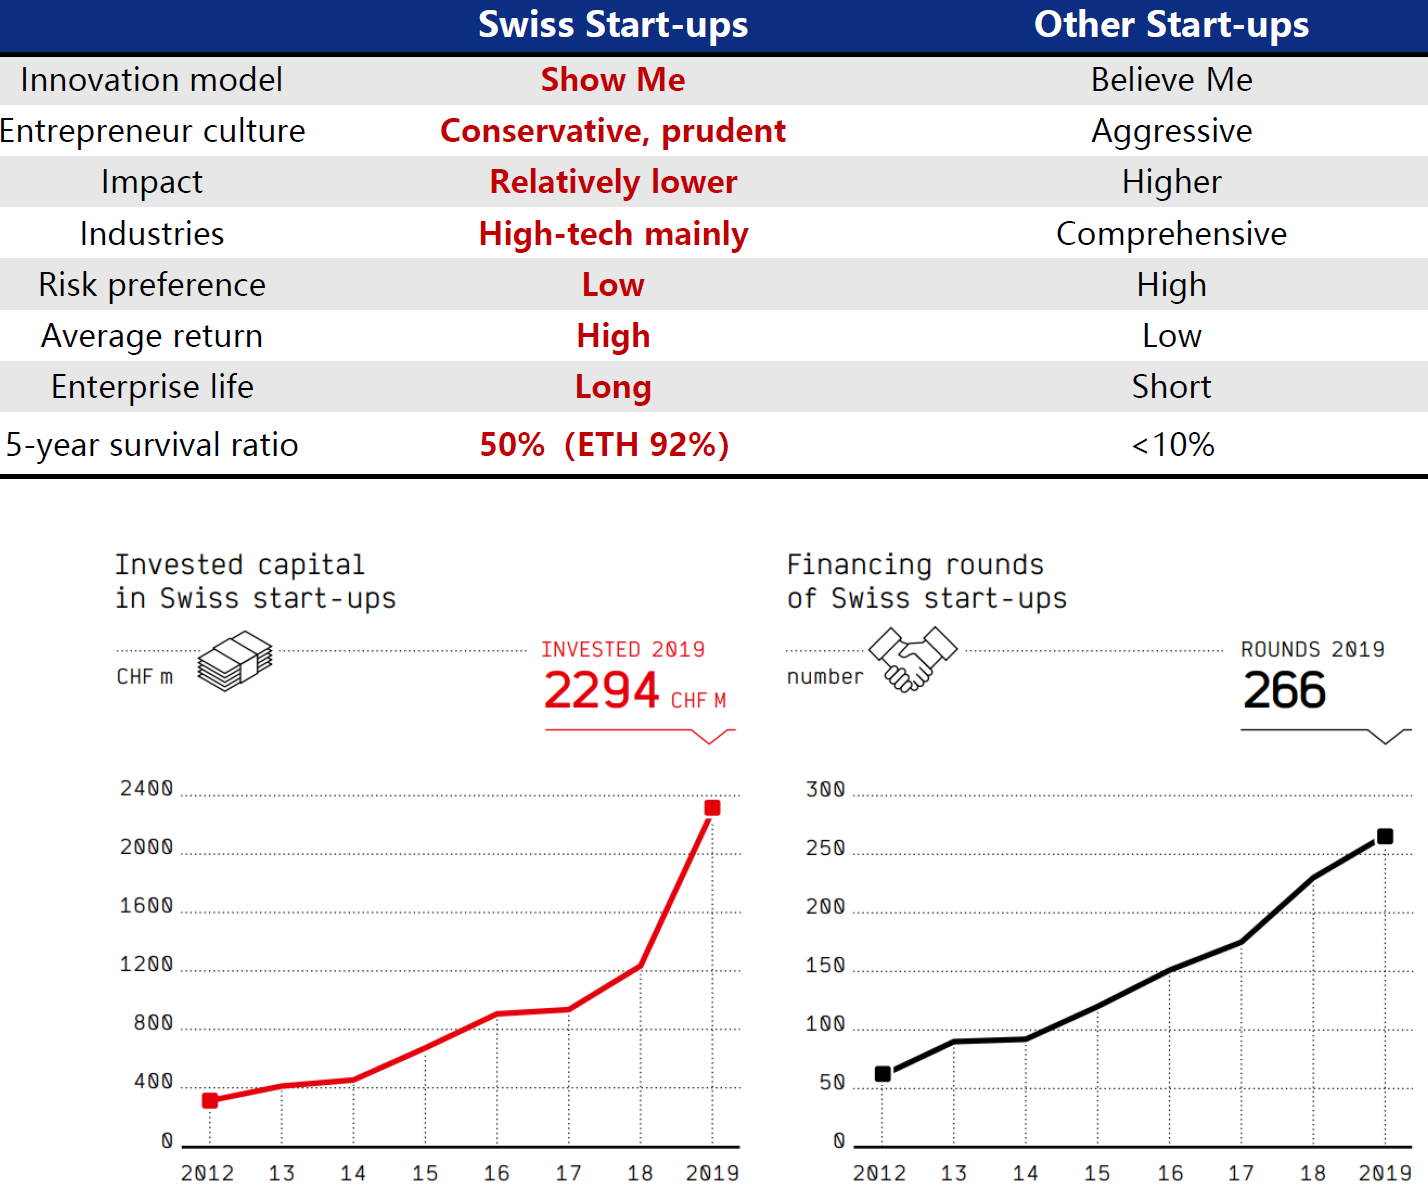
\includegraphics[width=0.7\textwidth]{Pictures/swiss_starups.png}
\end{figure}

Life sciences industry (including biotechnology, medical devices, health
information technology, eth.) as a traditional advantage industry remains
stable. The information and communications technology industry has risen
rapidly in recent years, with a significant growth rate, and the amount
of venture capital investment doubled in 2019.

\vspace{1\baselineskip}

From 2012 to 2018, the average amount of Swiss startup financing increased
by 26\% per year, reaching nearly 8.7 billion yuan in 2018, equivalent to
four times the amount of venture capital in 2012, and an average of 42 million
yuan per finanfing transaction.

Most Projects are very easy to get seed round funding and funds after the
A round, but the intermediate funding (between 2 million and 10 million
Swiss francs) is very difficult to obtain, which provides an excellent
opportunity for Chinese capital to cut in.

\begin{figure}[H]
    \centering
    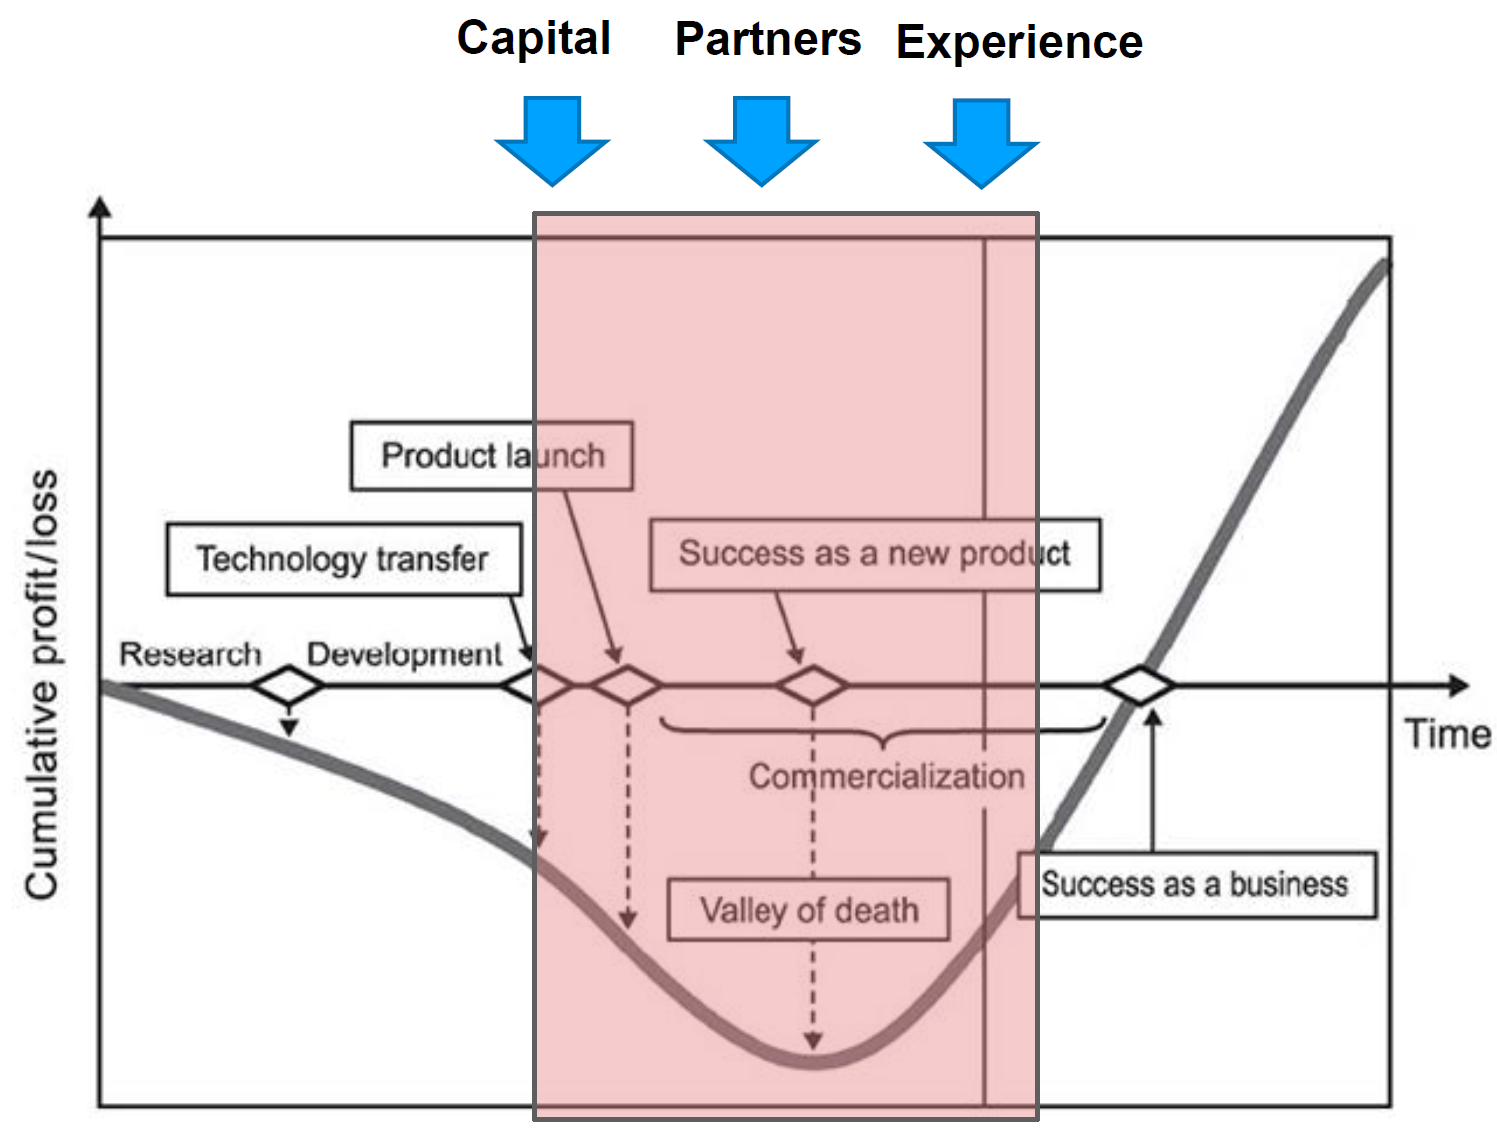
\includegraphics[width=0.45\textwidth]{Pictures/startup_lifecycle.png}
    \hspace{10pt}
    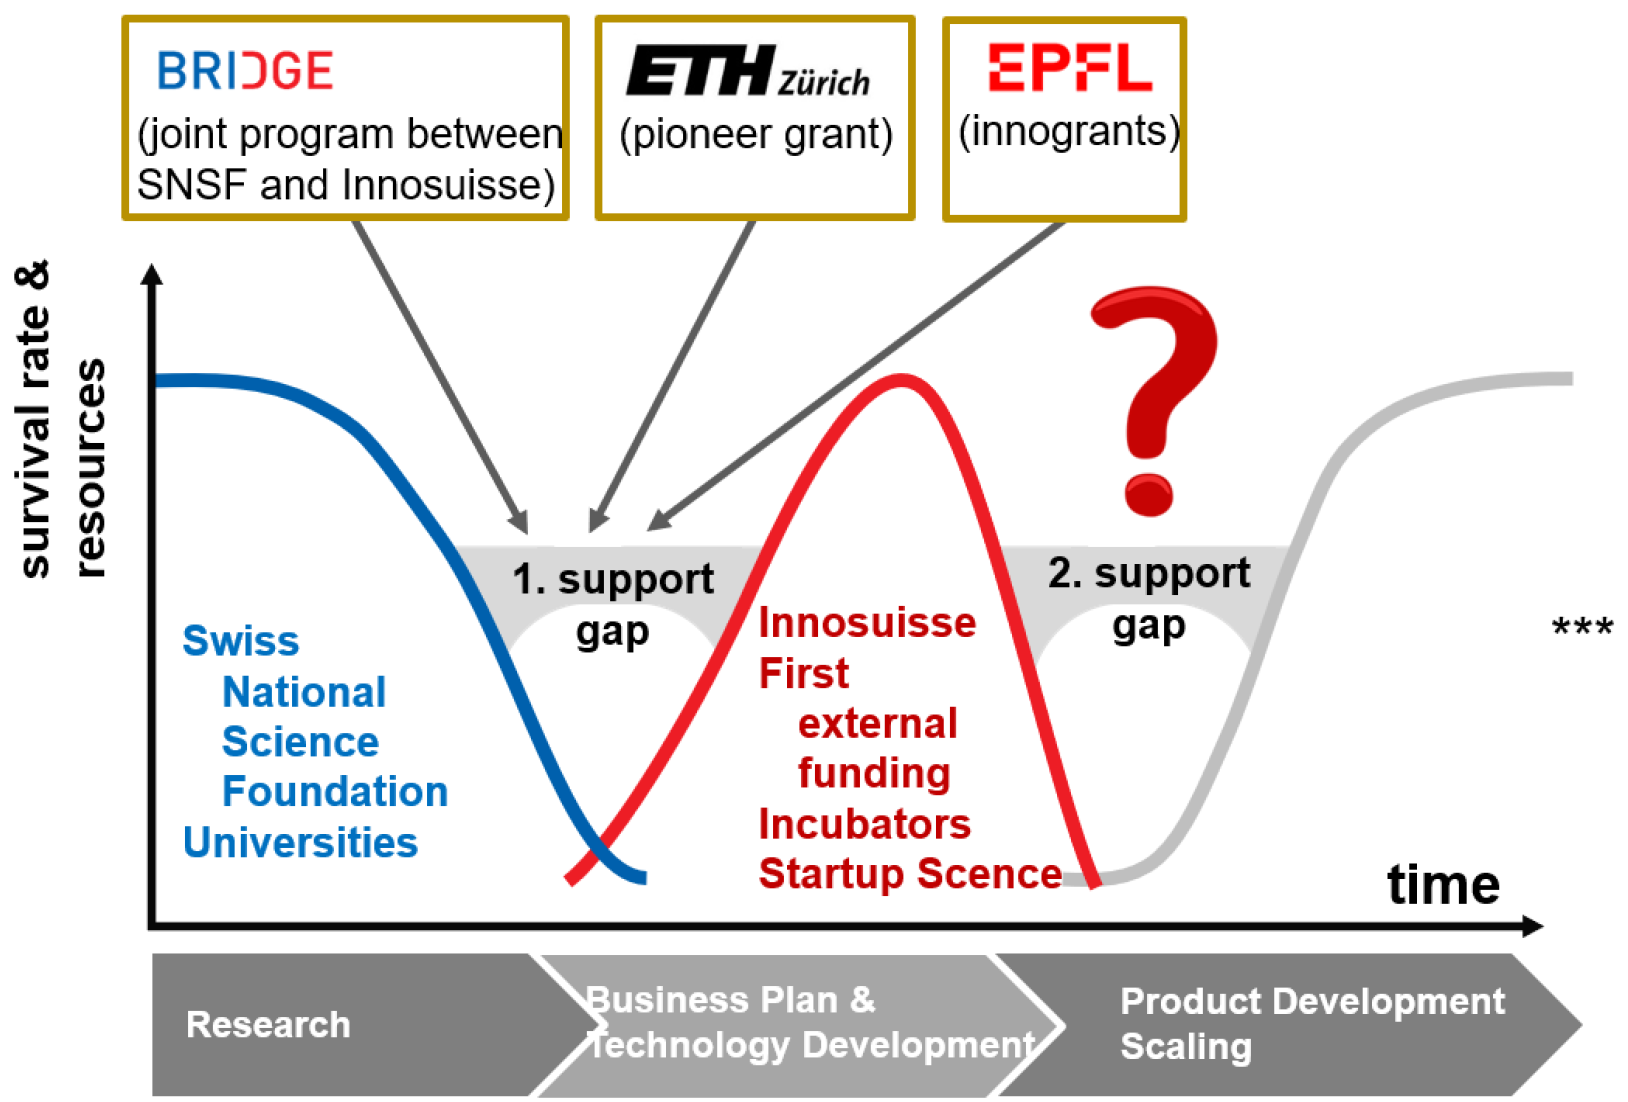
\includegraphics[width=0.45\textwidth]{Pictures/startup_lifecycle_2.png}
\end{figure}

\subsection{Chinese startups and innovation}

China's spending on research and development in science and technology,
surged ten-fold since 2000, while the US spending grew a modest 39\% in the
same period.

The chinese intellectual property protections grew over time just as in the
US just with a time shift of approximately 100-200 years.

\vspace{1\baselineskip}

Innovation refers ot the ability to produce new economic value through the
creation or improvement of products or business services. It can take many
forms. At one end of the spectrum is transformational innovation - something
that fundamentally alters a market or an industry. Often, but not always, it
is based on scientific research. But innovation can also be incremental - a
modification or enhancement to an exciting product or service that improves
its market position and increases its economic value.

\vspace{1\baselineskip}

China has advancced far beyond the mere copying of Western products or
technologies and now excels at incremental innovation. It still lags the US,
Europe, and Japan in transformational, science-based innovation, but with
a sustained policy focus and investment by its government and the leverage
provided by a massive domestic market, transformational innovation can also
be expected to advance.

\vspace{1\baselineskip}

Advances are clear at the national level, in fields such as supercomputing,
quantum communications, space, and robotics. In the private sector,
advances can best be seen in mobile commerve, where China currently leads the
world. While the innovations driving China's commercial success are mostly
incremental, they are increasingly enabled by investment in artificial
intelligence (AI). Outside of mobile commerce - in fields such as semiconductors,
software, commercial aircraft, and life sciences - China's advance is more
uneven. Even in those sectors, however, sustained investment is likely to
bring change.

\begin{figure}[H]
    \centering
    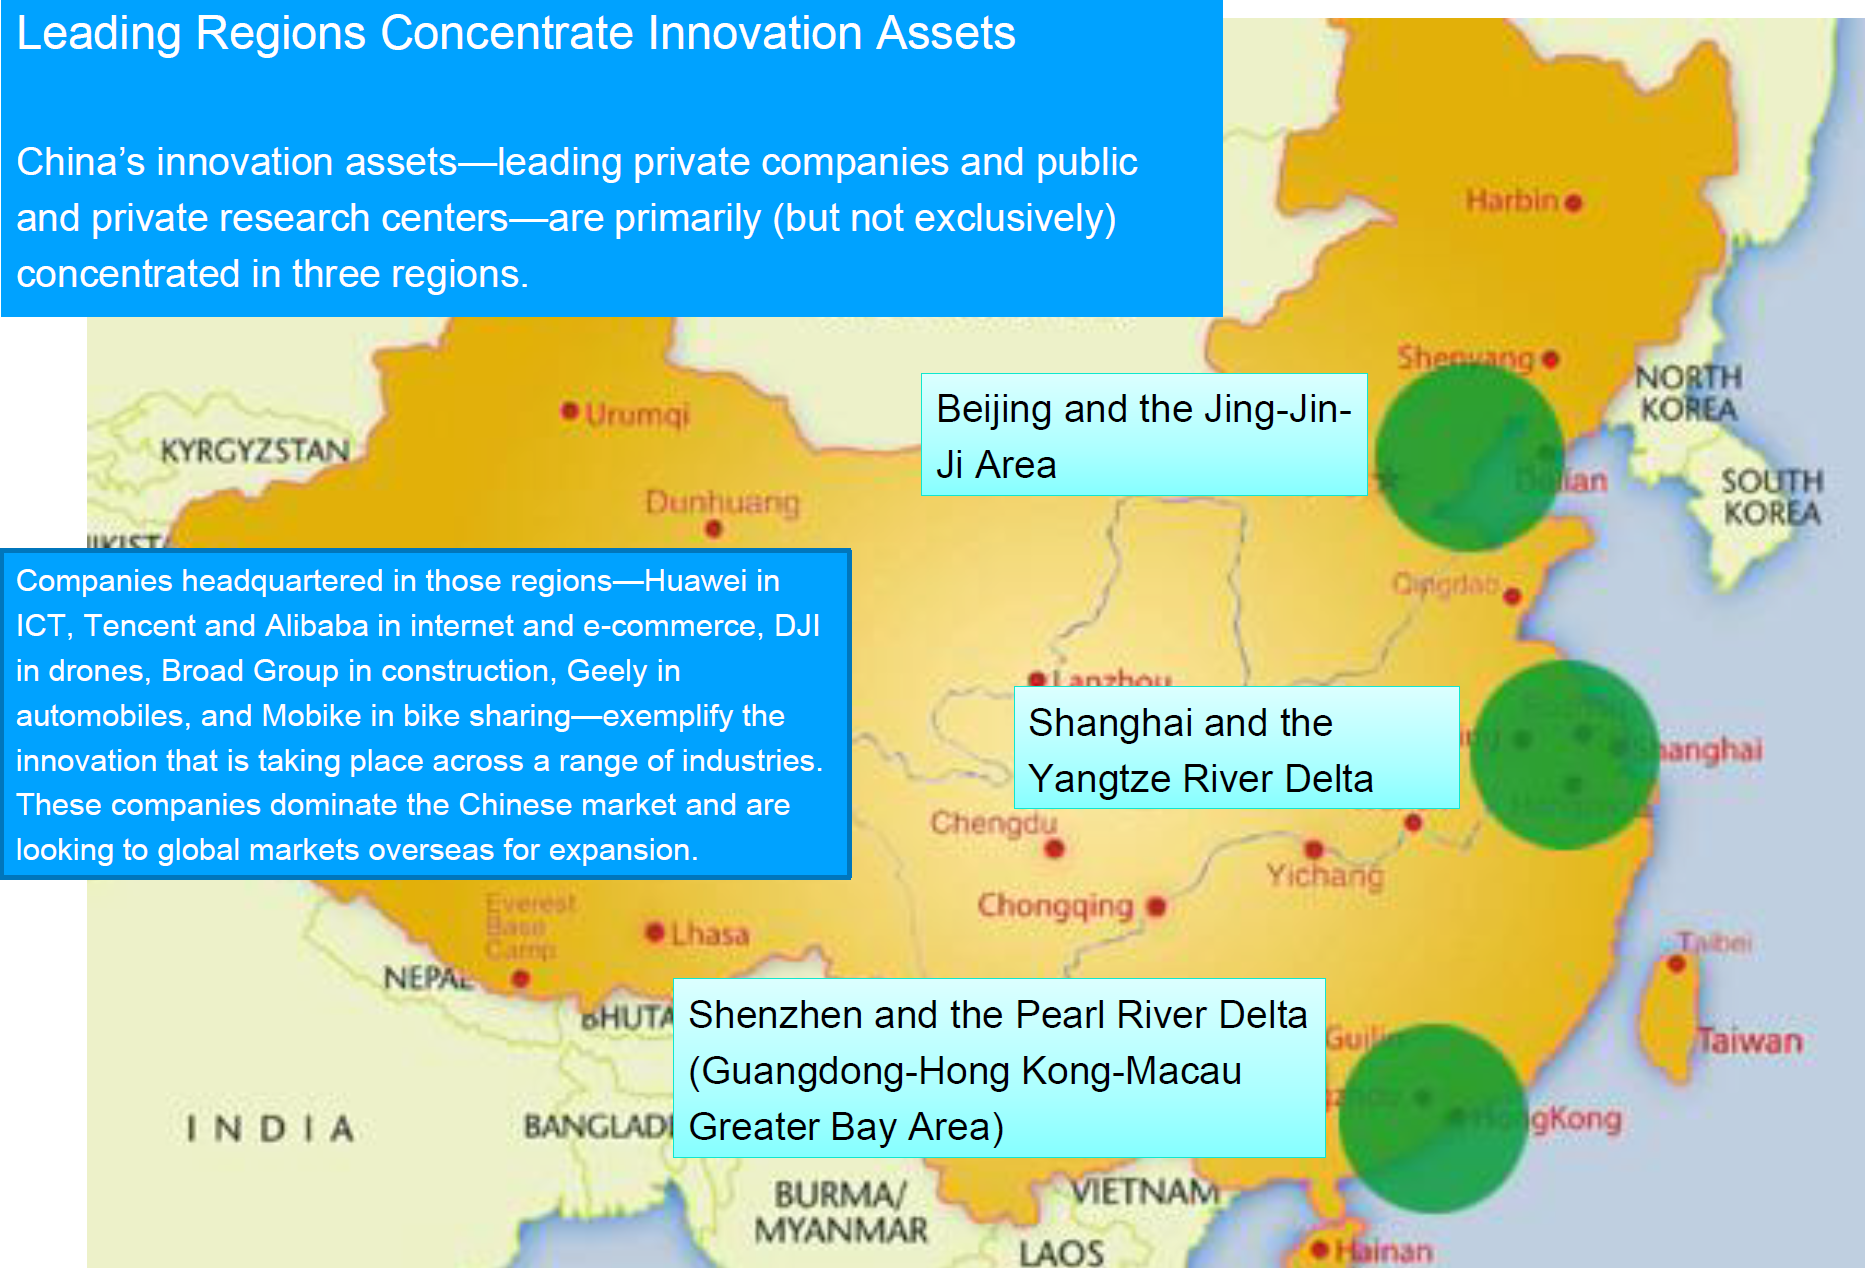
\includegraphics[width=0.65\textwidth]{Pictures/china_innovationhubs.png}
\end{figure}

China also has an increasingly robust starup scene, with a rapidly growing number
of incubators and accelerators. Many are sponsored by provincial and city
governments, offering benefits such as grants or free rent. It is not clear,
however, whether their rapid expansion reflects a similar scale of innovation,
or whether it constitutes a bubble.

\vspace{1\baselineskip}

There is also growing private investment in startups, by large companies such as
Tencent, Alibaba, and Baidu, and through an array of venture capital and private
equity firms. Reflecting the scale of this activity, in 2016 China let Asia in
the production of unicorns (companies with valuations of \$1 billion or more)
with 37; the country with the next largest number was India with 8. Internet
companies are receiving more than half of China's venture deal flow, and of
China's 46 unicorns in 2017, nearly half are backed by China's largest
internet companies.

\vspace{1\baselineskip}

Still, China's startup support ecosystem remains a work in progress. Venture
investors often look to monetize their investments quickly, reinforcing
tendencies in their portfolio companies to go for short-term gains instead
of transformational leaps (an area in which Silicon Valley excels). Most
Chinese universities are also behind the curve when its comes to programs that
generate and support Entrepreneur-led startups.

\vspace{1\baselineskip}

Not a lot of funding goes to early start-ups. Mainly the government invests
in companies which are before the IPO.

\vspace{1\baselineskip}

The ideology is that if your company fails, you disappoint the country becasue
the government invested in your company.

\vspace{1\baselineskip}

Despite several booms and busts in China's short venture capital history
(the 'capital spring' of 2014-2015 gave way to the 'capital winter' of 2016,
which then turned into the 'harvest year' of 2017), the number of private
venture capital institutions has grown from 10 in 1995 to 500 in 2005 and
5'000 in 2015. The composition of venture capital sources has changed over time.
Angel investments became abundant in 2014-2015, as a large number of wealthy
individuals joined the VC fray. With the tightening in 2016, more start-ups
turned to the newly established Third New Board for financing.

\paragraph{The 13th Five Year Plan}

Guiding government strategy for the 2016-2020 period, the 13th Five Year Plan
prioritizes indigenous innovation, the achievement of technological self-sufficiency,
the control of standards, and an expanded government role in the market. The
industries it prioritizes overlap with those targeted in Made in China 2025.
$\Rightarrow$ The 14th Five Year Plan (2021-2025)

\paragraph{Made in China 2025}

Made in China 2025 (MIC 2025) is an industrial policy designed to advance
China's global leadership in manufacturing by promoting indigenous innovation,
domestic brands, domestic standards, domestic production, the control of data.
Its scope reasserts the government's role in ventral economic planning in ways
that favor domestic companies over foreign ones in strategically selected sectors.
One of its many objecitves is the development of national corporate champions
that will one day become global market leaders. It does this in part by setting
global sales and market share targets for Chinese products, backed by directed
government resources. These resources can be used to fund foreign technology
acquisitions, among other purposes.

\paragraph{National Innovation-Driven Development Strategy Outline}

Products by the Central Committee of the Communist Party and the State Council
in 2016, the Outline lays out China's science and technology plans and policies,
promoting objectives similar to those of MIC 2025.

\begin{figure}[H]
    \centering
    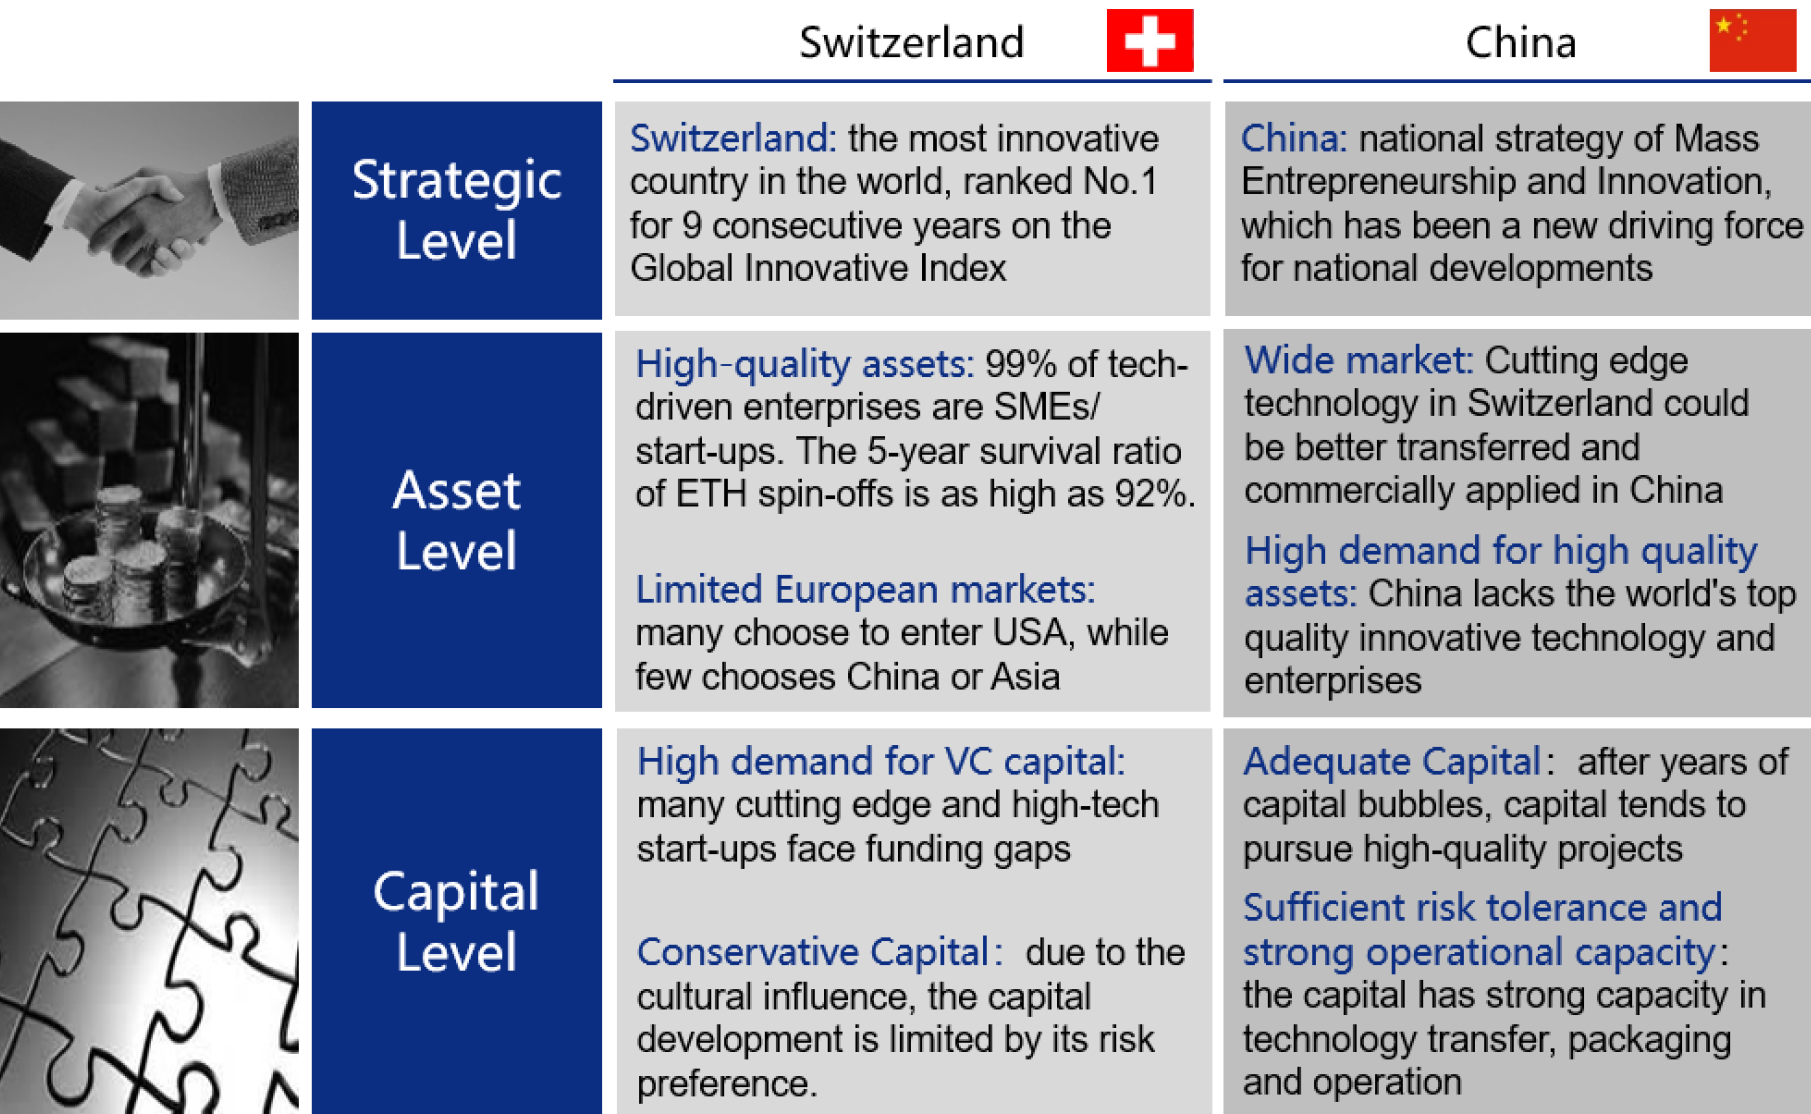
\includegraphics[width=0.7\textwidth]{Pictures/When_bottom_up_meets_top_down.png}
    \caption{When bottom-up meets top-down}
\end{figure}


\subsection{Opportunities}

See lecture Slides.\footnote{\url{https://xyotta.com/cfiles/1233}}

\vspace{1\baselineskip}

China's consumption growth over the next 15 years might be comparable with
that of the US and western Europe.

\begin{itemize}
    \item Wealth management
    \item Discretionary consumption
    \item Health
    \item E-commerce
    \item FinTech
\end{itemize}






\pagebreak

\section{Knowledge and economic growth. A history of discovery,
invention and innovation.}

\subsection{On the nature of economic growth}

\paragraph{How to measure economic growth}

Basics:
\begin{itemize}
    \item The output of an economy, in a specific counry, over a certain period,
        is measured in terms of GDP - Gross Domestic Product.
    \item GDP gives the monetary value of final goods and services - that
        are those bought by the final user (net of intermediate consumption)
    \item The simplest measure of economic growth is the annual increase
        of GDP.
    \item But it is better to correct for changes in inflation and population
        and use the annual increase of real GDP per capita as a proxy for
        economic growth.
\end{itemize}
GDP is a very crude measuere: It only counts transactions that can be given a
monetary value. Here are a few examples of what is excluded from GDP:
\begin{itemize}
    \item Unpaid houshold or voluntary work (on the positive side)
    \item So-called externalities like environmental destruction and
        pollution (on the negative side).
    \item Free digital goods like online search engines and new digital
        commons like Wikipedia or social media.
\end{itemize}

GDP is a short-term measure:
It only considers monetary transactions and flows and as such totally ignores
capital assets of all kinds such as the depletion of resources or loss of
biodiversity, nor does it account for the improvement, decay, or even destruction
of infrastructure or the value of human and social capital.

For example, the destruction of assets in wartime will not show up in GDP,
but the 'consumption' of weaponry and the reconstruction after the war will
boost GDP growth.

\paragraph{Economists understand little about the causes of growth}

\begin{itemize}
    \item growth is a consequence of capital accumulation (Solow,Swan,\dots)
    \item availability of land and resources\dots (taken for granted in a class
        of economic models)
    \item growth as a consequences of (Cobbs-Douglas) relations between labor,
        capital and technology; endogenous growth theories (Roman, Kramers\dots)
    \item growth made possible by legal and enforced framework (property rights)
    \item cultural and financial incentives for private efforts and innovations
    \item role of government, quality of governance and trust
    \item anti-corruption\dots
\end{itemize}

\paragraph{Exponential growth in the aggregate, with a rich underlying
dynamical process}

Using modern data analysis techniques, Lera and Sornette proved that economic
growth is bimodal:
\begin{itemize}
    \item With one regime of expansion with strong growth, and another regime
        of consolidation with low growth or decline.
    \item The system naturally switches between these two regimes in one single
        dynamical process.
    \item In this view, growth and consolidation are two sides of the same coin.
\end{itemize}

\paragraph{Secular bopolar growth rate of the real US GDP per capita.}
A long term average growth rate of real GDP per capita of 2\% per year is
obtained by regime shifts between regimes of high growth ($\sim 3\%$ per year)
and regimes of low growth ($<1\%$ per year).

Structural characteristics of growth: regime shifts and bimodal patterns

\subparagraph{Lesson 1:} Growth occurs in cycles and there is persistent
hubris in extrapolating the high-growth regimes

\vspace{1\baselineskip}

It is important to realize that:
\begin{itemize}
    \item The strong-growth modus is seen at the norm and the healthy state of
        economy, and the low-growth as an aberratoin and a symptom of disease
        that needs to be cured.
    \item Therefore, we always extrapolate the high-growth regimes.
    \item However, growth is a single bimodal process of overshooting during
        boom followed by correction and consolidation.
    \item The correction is as much part of the process as the boom.
\end{itemize}

To explain where the coarse-grained long-term exponential growth comes from,
we must first make a distinction between things and ideas, rival and nonrival
goods.

\paragraph{Things versus ideas}

Things (objects, goods) are rival:
\begin{itemize}
    \item As more people drive on a highway or use water for irrigation, there
        are fewer of these goods to go around\dots
    \item To increase the productivity of each person in an economic system using
        things (like a computer), you need to give each person such a thing.
        Economic output per capita, under such conditions, is proportional to
        the capital per person.
    \item in a closed economy, capital is subject to diminishing returns:
        'The first barrel of fertilizer does wonders for a plot of land; the
        tenth only burns the crop.'
    \item This leads to a kind of steady-state, end-of-growth, unless exogenously
        something happens (e.g. technological change)
\end{itemize}
Ideas, in contrast, are nonrival:
\begin{itemize}
    \item As more and more people use the Pythagorean theorem of the Java
        programming language, there is not less and less of the idea to go
        around.
    \item Ideas are not depleted by use, and it is technologically feasible
        for any number of people to use an idea simultaneously once it has
        been invented.
    \item You can increase the productivity of any number of people in an
        economic setting by inventing a single new idea. Economic output per
        capita, under such conditions, is proportional to the total stock of
        ideas. Taking logs and derivatives, the economic growth is proportional
        to the growth rate of the total stock of ideas.
\end{itemize}

\begin{figure}[h]
    \centering
    \begin{subfigure}{0.48\textwidth}
        \centering
        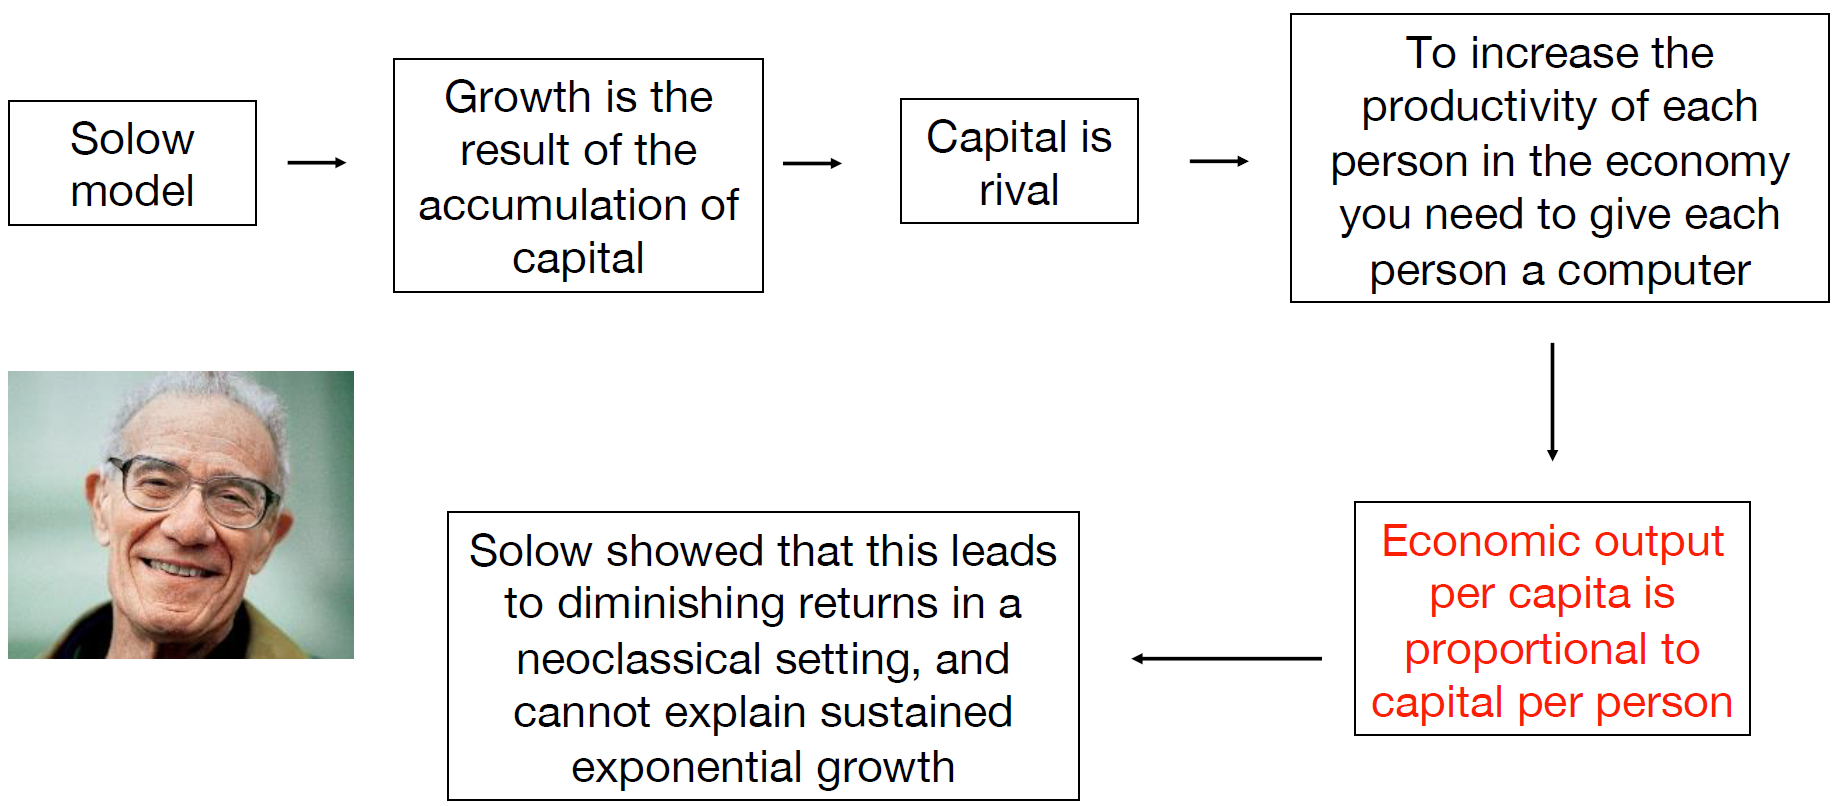
\includegraphics[width=\textwidth]{Pictures/Solow.png}
        \caption{Sollow Model}
    \end{subfigure}
    \hspace{5pt}
    \begin{subfigure}{0.48\textwidth}
        \centering
        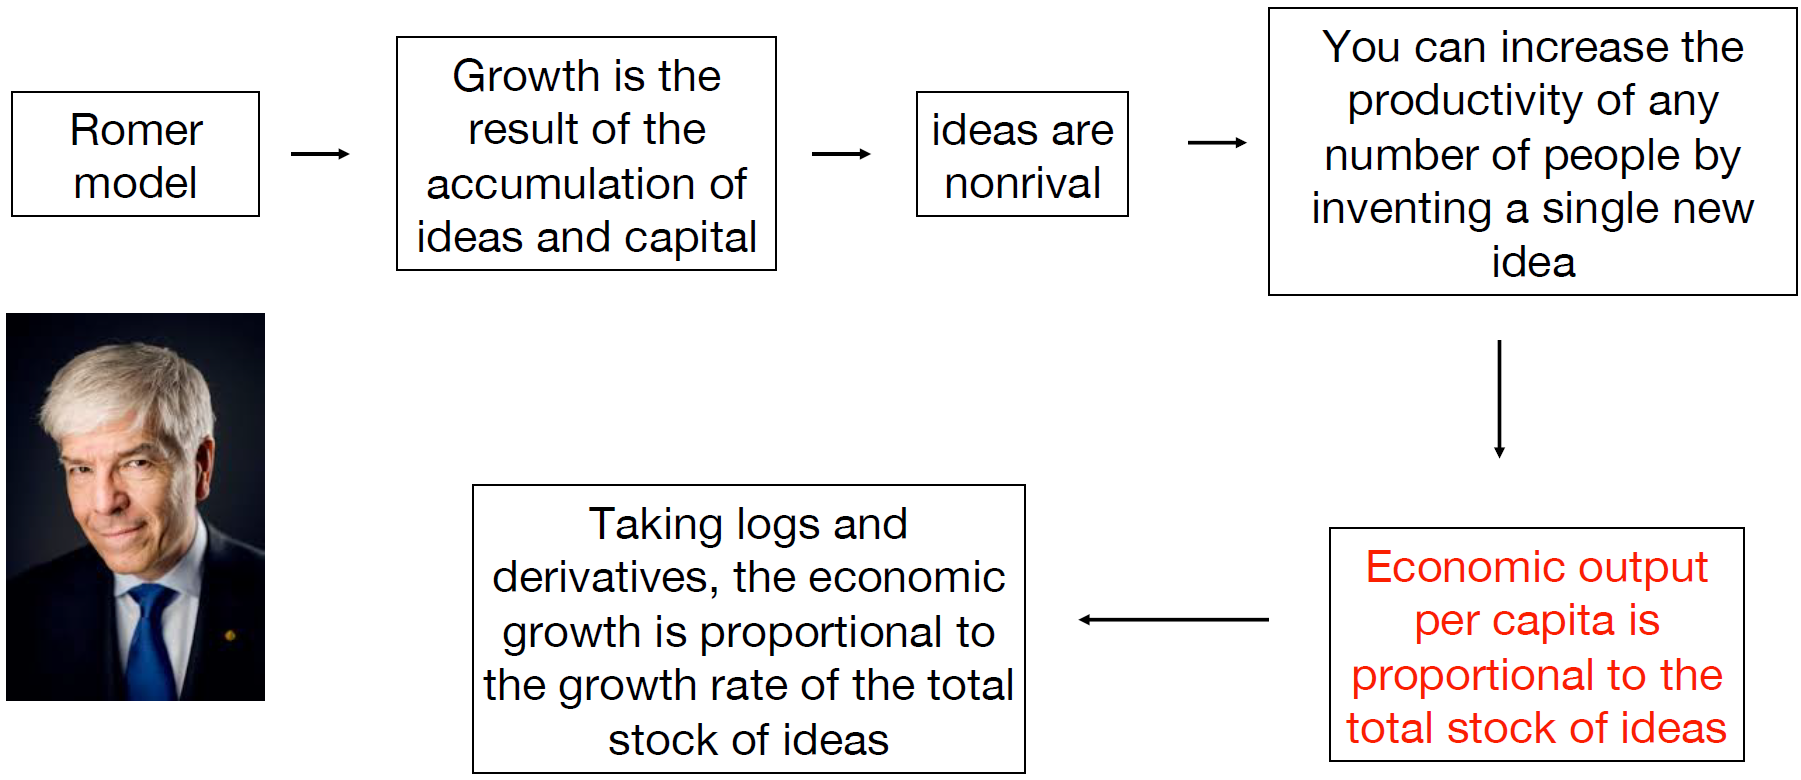
\includegraphics[width=\textwidth]{Pictures/Romer.png}
        \caption{Romer Model}
    \end{subfigure}
\end{figure}

\paragraph{Endogenous growth theory}

\begin{itemize}
    \item Economic growth is proportional to the growth rate of the overall
        stock of ideas.
    \item The overall stock of ideas grows with the increase of resources
        allocated to finding new ideas (people, capital,\dots)
    \item But it plateaus when ideas become harder to find (S-curve, logistical
        process\dots)
    \item The economy can only grow at a constant rate over the long run if
        research productivity (output/input, or results/investment) is
        constant.
\end{itemize}

In the following parts, we will zoom in on the following three questions:
\begin{itemize}
    \item Are ideas harder to find?
    \item What exactly is 'knowledge'?
    \item Is there a constant rate of knowledge accumulation?
\end{itemize}

\subsection{On the productivity of research}

Discussing question 1: 'Are ideas harder to find?'

\vspace{1\baselineskip}

Despite vast increase in in the time and money spent on research, progress
is barely keeping up with the past. What went wrong?

\vspace{1\baselineskip}

Number of PhD students increase and more is invested in research. On the surface,
this is encouraging. But for all this increase in effort, are we getting a proportional
increase in our scientific understanding? Or are we investing vastly more
merely to sustain (or even decline in) the rate of scientific progress?

\vspace{1\baselineskip}

Economic growth (e.g. 2\% or 5\%) = Research productivity (falling) $\times$
Number of researchers (rising)

\vspace{1\baselineskip}

To have a constant research productivity, the effective number of researchers
and the US TFP growth should behave similarly. It turns out that we need more
than $20 \times$ more research capacity (input), to sustain a declining
productivity (output).

\vspace{1\baselineskip}

\paragraph{Are ideas getting harder to find?}

In a paper in the American Economic Review, Bloom et al. give some compelling
evidence:
\begin{itemize}
    \item Moore's law: 'the number of researchers required to double chip density
        today is more than 18 times larger than the number required in the early
        1970s\dots Research productivity in this case is declining sharply, at
        a rate of 7\% per year.'
    \item Research productivity for crop seed yields and mortality improvements
        associated with cancer and heart diseases declines at a rate of 5\% per
        year.
    \item Looking at firm-level data, research productivity declines at a rate
        of 8-10\% per year dependent on the data source.
\end{itemize}

\paragraph{But continuous increase in R\&D investment}

Over the past 70 years, the non-financial business debt in the U.S., as a
fraction of GDP has increased from 40\% to 140\%. However, the contribution
of investments to GDP has hovered between 15\% and 20\%.

Where has the increasing debt of American businesses been used for, if not
for CAPEX and fixed assets?

The most probable answer is that this debt is used to finance goodwill
(e.g. from M\&A activity) and intangible assets (R\&D, patents,\dots)

\subsection{On the nature of knowledge}

Discussing question 2: 'What exactly is knowledge?'

\subsubsection{What is "knowledge"?}

What is the difference between discovery, invention and innovation?

\paragraph{Discovery}

The first-time recognition of something already existing:
\begin{itemize}
    \item \underline{A thing}: a new mine or an oil well, a continent, an
        island, a moon, planet, star, a fundamental particle (such as the
        electron or a neutrino)\dots
    \item \underline{An idea}: an insight, like the discovery of a fundamental
        law of nature.
\end{itemize}

The result of a process of exploration:
\begin{itemize}
    \item A high-risk endeavor into the unknown
    \item Willingness to employ substantial expenses without any certainty
        for future results or returns.
\end{itemize}

To use the words of the opening lyrics of the Star Trek television series,
discovery is 'to boldly go where no man has gone before'.

\subparagraph{The challenges of exploration}
According to Herbert Simon exploration requires:
\begin{itemize}
    \item tolerance of ambiguity
    \item patience: learning-by-doing, accumulation of knowledge, trial-and-error
    \item luck / serendipity
    \item persistence / dilligence
    \item 'intuition': use of smart heuristics
\end{itemize}

It is a high risk endeavor, where the payoff is almost impossible to estimate.

\paragraph{Invention}

The creation of something new:
\begin{itemize}
    \item \underline{A thing}: a mechanical machine like a steam engine, a
        scientific instrument like a microscope
    \item \underline{An idea}: a mathematical algorithm, like artificial
        intelligence, or chemical process like the Haber-Bosch ammonia
        synthesis to produce fertilizers, or the Bessemer process to decarbonize
        iron in the production of steel.
\end{itemize}

The result of a creative process:
\begin{itemize}
    \item Engineering
    \item often combined with stubborn trial-and-error tinkering
    \item and a large dose of luck
\end{itemize}

\paragraph{Innovation}

Combining existing things and ideas in a novel way to:
\begin{itemize}
    \item Solve a problem,
    \item optimize a process
    \item or bring a new products or service to the market.
\end{itemize}

The result of a process of exploitation:
\begin{itemize}
    \item Taking advantage, by doing combinatorics, of prior creative inventions
        and explorative discoveries
    \item Low (or at least known) risk endeavor into charted territory
    \item where one can make a decent estimation of the prospect of success
\end{itemize}

\subsection{How do we innovate, invent or discover?}

How to understand the incentives?

\paragraph{The whole is greater than the sum of its parts}

$R \sim c^\beta$ where the production $R$ is defined as the total number
of commits measured per 5-day time window for the Apache Web server and
$c$ is the number of active contributors in the same 5-day time window.
$\beta$ decreases with increasing number of developers.

\vspace{1\baselineskip}

Six design principles to help managers deal with the challenge of
Productive/Creative Bursts.
\begin{enumerate}[1)]
    \item transparency
    \item bottom-up incentives and self-censored clans
    \item emergent technology
    \item problem front-loading
    \item distributed screening
    \item Modularity
\end{enumerate}

\paragraph{The skill-success gap}

Mechanisms of Luck
\begin{itemize}
    \item Gibrat's law, proportional growth, and the Matthew effect
    \item Winner-takes-all
    \item Adverse selection
    \item Male-male competition and evolution
    \item Big statistic replication crisis
    \item Hyped big data, artificial intelligence, and machine learning
\end{itemize}

\paragraph{Skill versus luck}
\begin{align*}
    \frac{d S_t}{S_t} = \mu dt + \sigma d W_t
    \hspace{10pt} , \hspace{10pt}
    \ln(S_t) \sim \klammer{\mu - \frac{\sigma^2}{2}} T + x_i \sigma \sqrt{T}
\end{align*}
\begin{itemize}
    \item $S$, the size of a firm
    \item $\mu$, the growth rate
    \item $W$, Wiener process, stochaistic random noise
    \item $\sigma$, volatility
    \item $\mu_{skill}$, the mean of the skills of the $N$ agents
    \item $\sigma_{skill}$, the standard deviation of the skills of the $N$ agents
    \item $\mu_{luck}$, the mean of the luck of the $N$ agents
    \item $\sigma_{luck}$, the standard deviation of the luck of the $N$ agents. 
\end{itemize}
There is a characteristic time $T^\ast$ at which skill and luck will contribute
equal the outcome of the GBM process. At that time $T^\ast$ satisfies $\mu T^\ast
= \sigma \sqrt{T}$, yield $T^\ast = \klammer{\frac{\sigma}{\mu}}^2$.

\vspace{1\baselineskip}

Sharpe ratio - see lecture slides 26.05\footnote{\url{https://xyotta.com/cfiles/1236}}

\subsection{The industrial revolutions, four waves of industrial innovation}

Is there a constant rate of knowledge accumulation?

\begin{enumerate}[]
    \item \underline{Industry 1.0}: The Industrial Revolution begins.
        Mechanization of manufacturing with the introduction of steam and
        water power.
    \item \underline{Industry 2.0}: Mass production assembly lines using
        electrical power.
    \item \underline{Industry 3.0}: Automated production using electronics,
        programmable logic controllers (PLC), IT systems and robotics
    \item \underline{Industry 4.0}: The 'Smart Factory'. Autonomous decision
        making of cyber physical systems using machine learning and Big Data
        analysis. Interoperability through loT and cloud technology.
\end{enumerate}

\paragraph{Industry 1.0} The industrial revolution (1760-1840)

Technology:
\begin{itemize}
    \item Mechanization of manufacturing with the introduction of machine tools
        and steam power
    \item Mainly focused around the textile industry (cotton, wool, silk) e.g.
        spinning jenny
\end{itemize}
Energy:
\begin{itemize}
    \item Beginning of the use of coal to power steam engines (steam power),
        in addition to muscular power (animals and humans) and traditional
        biofuels.
\end{itemize}
Geography:
\begin{itemize}
    \item Originally started in the UK
\end{itemize}
Infrastructure:
\begin{itemize}
    \item Networks of canals and improved waterways
    \item Paved 'macadamized' roads (John McAdam)
    \item First introduction of railroads in the UK (ending in the Railway
        Mania of the 1840s)
\end{itemize}

\paragraph{Industry 2.0} The technological revolution (1870-1910)

Technology:
\begin{itemize}
    \item Electricity: steam turbine, generator, transformer, engine, incandescent
        bulb, light
    \item Steel (Bessemer process)
    \item Combustion engine
    \item Chemistry: synthesis of new materials and chemical products
\end{itemize}
Management:
\begin{itemize}
    \item Economy of scale: It is cheaper to manufacture products in large quantities
    \item Vertical integration of the supply chain from raw materials (e.g. iron
        ore and coal) to final product (e.g. steel railway track)
    \item Scientific management (Taylorism): new empirical organization methods
        to improve efficiency and labor productivity in large scale businesses
        that operate over vast areas.
\end{itemize}
Geography:
\begin{itemize}
    \item US, UK, Continental Europe
\end{itemize}
Energy:
\begin{itemize}
    \item Coal and the birth of the high energy society
\end{itemize}
Infrastructure:
\begin{itemize}
    \item Networked house (electricity, sewage, streaming water, telephone,
        central heating, etc)
    \item Electrified underground railways (Paris Métro, London Tube, Berlin U-Bahn,\dots)
    \item Linking of existing railway networks to allow for long-distance
        travelling (e.g. Paris-Istanbul with orient express, Moscow-Vladivostok
        with Trans-Siberian Railway,\dots)
    \item Transatlantic telegraph cable
    \item Transcontinental steamhip routes
    \item Sea canals (Suez, Panama)
    \item City planning
\end{itemize}

\vspace{1\baselineskip}

\begin{itemize}
    \item New structural forms with the application of new engineering techniques and
        materials such as glass and steel.
    \item The rise of the modern city: straight boulevards, buildings with equal
        hights, parks and squares, new sewer systems, infrastructure for fresh
        drinking water\dots
\end{itemize}

\paragraph{Industry 3.0} The electronic revolution (1947-20xx)

Technology:
\begin{itemize}
    \item PLC (Programmable Logic controllers)
    \item Computers (transistor, Integrated circuits, computer chips, microchips)
    \item Software and computer programs, user interfaces
    \item Robotics
    \item Mobile phones / smartphones
\end{itemize}
Infrastructure
\begin{itemize}
    \item Automobile: Interstate highway systems
    \item Aircraft: Jet Age (aircraft powered by turbine engines),
        Long-distance commercial flights
    \item Digital: internet, worldwide web
    \item Mobile
\end{itemize}
Energy
\begin{itemize}
    \item Oil and gas
    \item Nuclear
\end{itemize}

\begin{enumerate}[]
    \item \underline{Phase 1}: Mainframe computers connected through ARPANET
        (US department of defense) in TCP/IP protocol $\rightarrow$ internet
        mainframe
    \item \underline{Phase 2}: Desktop, laptop, tablets and smartphones connected
        in WWW (HTMP - HyperText Markup Languate, invented in CERN) $\rightarrow$
        internet of people, data and services
\end{enumerate}

\paragraph{Industry 4.0} The cyber revolution (20xx - \dots)

Phase 3: Cyber Physical Systems $\rightarrow$ internet of everything

\vspace{1\baselineskip}

People to people, people to machines and machines to machines

\vspace{1\baselineskip}

Technology: Cyber physical systems: physical and software components are
deeply interwined
\begin{itemize}
    \item Machine to machine technology
    \item Smart: Things measure, analyse and act autonomously
    \item Self-organization of technology, machines, human beings\dots
    \item internet of things
    \item Sensors
    \item Artificial intelligense, algorithms, big data analysis
    \item Augmented reality
    \item Additive manufacturing
    \item Cloud computing
\end{itemize}

\subsection{A critical assessment of the industry 1.0 : 4.0 framework - The
Chinese case}

\begin{itemize}
    \item It is very much Western-centric and describes technological progress
        as a continuous and steady process, from industry 1.0 up to industry
        4.0, like the different deployments of a software package.
    \item In reality, progress (in technology, economy, society,\dots) is
        discontinuous and punctuated
\end{itemize}

\paragraph{Han Dynasty in China} (207 BCE - 9 CE) The achievements of the Han
dynasty in the field of science and technology were concentrated in hydroproject,
architecture, mathematics, calendars and other technological fields, Han dynasty
witnessed some of the most significant advancements in premodern Chinese science
and technology. 'The consatenation of Han advances laid strong technical foundations
for the development of the world's most persistent empire - which was, until the
18th century also the world's richest economy\dots'

\paragraph{Boreholes and mining shafts} (206 BC - 220 AD)
Borehole drilling has a long history. By at least the Han Dynasty, the
Chinese used deep borehole drilling for mining and other projects. The Chinese
method of deep drilling was accomplished by a team of men jumping on and off
a beam to impact the drilling bit while the boring tool was rotated by buffalo
and oxen. By the first century BC, Chinese craftsmen cast iron drill bits and
drillers were able to drill boreholes up to 1500 m deep. It wasn't up until
the 19th century that Europe and the West would catch up and rical ancient
Chinese borehole drilling technology.

\paragraph{Hydraulics} (206 BC - 220 AD)
By the Han Dynasty, the Chinese developed various uses for the waterwheel. In
his Balanced Discourse, the philosopher Wang Chong first described the square-pallet
chain pump that could pump water and other substances. Their primary use was for
lifting water into irrigation ditches, but chain pumps were also used in public
works programs, such as when Zhang Rang used them to lift water into pipes.
The water was used to provide the capital Louyang with clean water. In 31 AD
Du Shi is credited with being the first to apply hydraulic power to operate bellows
(air-blowing device) in metallurgy. This is a great invention in ancient China
and the history of mechanical engineering, about a thousand years earlier
than Europe.

\paragraph{The Seismograph} (132 BC)
The Han court was responsible for the major efforts of disaster relief when natural
disasters such as earthquakes devastated the lives of commoners. Zhang Heng, an
early Chinese scientist, created the first device for detecting distant earthquakes
had occured in a location indicated by a specific cardinal or ordinal direction,
which he introduced in the Han court in 132 AD. Its design was simple - an urn
equipped with a pendulum. When it picked up a vibration, it dropped a ball from
the mouth of a metal dragon into a metal frog, creating a loud clang. The first
time that happened, nobody in the court reportedly felt anything, but a few
days later, a messenger from a villate 400 miles away arrived to inform the
emperor that an earthquake hat occured there.

\paragraph{The Wheelbarro} (100 BC)
The Wheelbarrow was developed in China perhaps as early as 100 BC. It can
acconodate a much larger wheel, thus reducing the rolling resistance, and by
having the wheel almost directly under the load it reduced the weight on the
user's arms.

\paragraph{The Invention of Paper} (105 AD)
Cai Lun, an eunuch in the Han court in 105 AD, is credited as the inventor of
the first really high-quality writing paper, which he fashioned by crushing
and combining tree bark, hemp, linen rags, and scraps from fishing nets and
then treating the mixture with lye to break it down into finer fibers.

\paragraph{Longshou Canal} (120-111 AD)
The Longshou Canal was built in 120 BC - 111 BC during the Han Dynasty, which
is the first underground canal in China's history with more than 5 km, the
Longshou Canal making use of the shaft-tunnel method. Its completion allowed
irrigation of more than 40,000 hectares of saline land and increased the yield
of its farmland by more than 10 times. This hydoproject method spread to Central
and Southwest Asia through the Silk Road. The Longshou canal has provided
valueble experience for the world's water conservancy industry.

\paragraph{Gunpowder weapons in the Song dynasty} (969-1044 AD)
The earliest-known existent written formulas for gunpowder come from the
Wujing Zongyao text of 1044, which described explosive bombs hurled from
catapults. The earliest developments of the gun barrel and the projectile-fire
cannon were found in late Song China. These 'fire-lances' were widespread in
use by the early 12th century, featuring hollowed bamboo poles as tubes to
fire sand particles (to blind and choke), lead pellets, bits of sharp metal
and pottery shards, and finally large gunpowder-propelled arrows and rocket
weaponry.

\paragraph{Hydraulic-powered astronomical clock tower}
Created by Su Song of the Song Dynasty in 1088 AD, it has three functions of
observing the movement of the celestial bodies, demonstrating the changes in
the sky, and accurately telling the time. It is the oldest astronomical clock
in the world, representing the wisdom of polymaths and mechanical engineering
of the Song Dynasty.

\paragraph{Jiaozi - The first paper money in history} (1023 AD)
Jiaozi, the earliest paper money used in the world, first appeared in the
Sichuan region and was issued in Chengdu in 1023. In the beginning, the Jiaozi
was actually a certificate of deposit, with the development of the market economy,
the use of Jiaozi became more and more widespread, and in a short time it turned
from a commercial credit certificate into an official legal currency with all the
basic elements of modern paper money. Compare with western, the first
government-issued paper money in the western world was in the late 17th century,
more than 600 years after China.

\subsection{A critical assessment of the industry 1.0 : 4.0 framework}

Are the 4 different periods equal? Do they represent the same amount of "progress"?
Maybe some inventions are more important than others?

\vspace{1\baselineskip}

Clean water and better hygene lowered the death rate extremely. Older inventions
such as amnesthetics is much more important than for example VR gogglles for
user experience. New inventions replaced older ones. Fake news are nothing
new.

\subsection{Conclusion}

We discussed the followign three fundamental questions.
\begin{itemize}
    \item Are ideas harder to find? Yes
    \item What is the meaning of knowledge? Semantics do matter, knowledge
        itself has a fine-grained structure and should be disentangled into
        discovery, invention and innovation.
    \item Is there a constant rate of knowledge accumulation? No, it follows
        a complex process with ruptures, paradigm shifts, revolutions
\end{itemize}
It seems that the puzzle of economic growth has not been solved completely yet.
And maybe a next step forward could be found through a better understanding
of the structure and the dynamics of the knowledge accumulation process.

\subsection{In our research group, we are trying to contribute to solving this
puzzle. Here are some very recent results}

\paragraph{Is there a constant rate of knowledge accumulation?}
\begin{itemize}
    \item We assembled a prioritary dataset of great inventors and discoverers
        over the past two milennia.
    \item You can see peeks in the graph during the industrial revolutions
\end{itemize}

\paragraph{Knowledge is not homogeneously distributed in space or time and across
scientific disciplines}

\begin{itemize}
    \item In time, a rich pattern of waves can be observed coinciding with industrial
        and technological revolutions and scientific paradigm shifts.
    \item In space, we see that the UK has been the major participant in the three
        industrial revolutions from the past 250 years, in the first half of that
        period, the European Continent was its main challenger; in the second
        half it was the US. It is eye-opening to see that European Continent's
        steady decline since the 1900s, except perhaps in biology, medicine
        and genetics.
    \item Across scientific disciplines, we see a general superiority in physics,
        mathematics and astronomy, a long-term decline in Chemistry, and a strong
        increase in biology, medicine in genetics between 1910 and 1970.
\end{itemize}
Since 1970 all disciplines are in decline across all geographical regions. Our
data would suggest that industry 4.0 is fully driven by innovation, and that
the rate of discovery and invention is in a secular decline. Could this be one
of the fundamental drivers behind dynamics of the Fool's Gold Age?

\subsection{How to quantitatively formulate the problem of exploitation of an
existing set of invention,innovation and exploration}

\paragraph{What is the investment universe?}

\begin{itemize}
    \item The vast majority of papers on portfolio selection starts with a
        sentence of the form 'The investment universe consists of one risk-free
        and $N$ risky assets'.
    \item In practice, even if $N$ is large, it is arguably not the case that
        the $N+1$ assets present in the specified investment universe cover
        every conceivable investment opportunitiy for the agent. Large investors
        are continuously looking for new investment opportunities (private
        investment, start-ups, crypto-assets, etc)
    \item Rather, these are the investment opportunities which are salient
        to the agent and well understood in terms of their relevant distributional
        properties.
\end{itemize}

\paragraph{Exploration of new investment opportunities}
\begin{itemize}
    \item We propose an extension of the classical setting with a fixed
        investment universe by giving the agent the option to explore for new
        investment opportunities.
    \item If this option is exercised, the agent chooses to devote a part of
        his/her wealth for exploration.
    \item Exploration results in the discovery of a new asset, whose distribution
        properties depend on the amount devoted to exploration in a way that the
        asset becomes more attractive to the agent when a larger amount is devoted
        to exploration.
    \item After discovery of the new asset, the agent of the extended investment
        universe in order to optimize her preferences over the resulting
        terminal wealth.
    \item trade-off between exploration and exploitation
\end{itemize}
\paragraph{Investment setting}
\begin{itemize}
    \item We consider a single-period model of an agent with mean-variance
        preferences.
    \item Classical model: dixed investment universe $\mathcal{U}$ consisting
        of a risk-free bond providing a deterministic return $r_f$ and $N$
        risky stocks with random return $\overline{r} = (r_1,\dots,r_N)'$.
    \item Under mean-variance preferences, knowledge about the mean and
        covariance structure of the risky assets is sufficient for portfolio
        analysis. We assume that $r \in L^2(\mathds{P})$ and let $\overline{r}
        := \mathds{E}[r]$ and $\Sigma := \mathds{E} \eckigeklammer{(r-\overline{r})
        (r-\overline{r})'}$
    \item We suppose that $\Sigma$ is positive definite and that $\overline{r}
        \neq r_f \mathds{1}_N$, where $\mathds{1}_N \in \R^n$ denotes the
        vector with all components equal to one. 
\end{itemize}
\paragraph{Classical mean-variance optimization problem}
In the standard setting, an agent with initial wealth $x_0$ and target expected
return $\mu \geq r_f$ solves classical mean-variance optimization problem
\begin{align*}
    \min_{u \in \R^n,u_0 \in \R} u' \Sigma u
    \hspace{10pt} \text{such that} \hspace{10pt}
    u' \overline{r} + u_0 r_f = \mu x_0
    \hspace{5pt} \text{and} \hspace{5pt}
    u' \mathds{1}_N + u_0 = x_0
    \hspace{30pt}
    (MV(\mu,x_0))
\end{align*}
Recall the following constants associated with the investment universe
$\mathcal{U}$,
\begin{align*}
    A = \mathds{1}_N' \Sigma^{-1} \overline{r}
    \hspace{10pt} , \hspace{10pt}
    B = \overline{r}' \Sigma^{-1} \overline{r}
    \hspace{10pt} , \hspace{10pt}
    C = \mathds{1}_N' \Sigma^{-1} \mathds{1}_N
    \hspace{10pt} , \hspace{10pt}
    D r_f^2 C - 2 r_f A + B
\end{align*}
which play a role in the explicit derivation of the optimal value and optimal
solution to $(MV(\mu,x_0))$. The optimal value of $(MV(\mu,x_0))$ is given by
$\sigma^2_{MV} = \frac{(\mu - r_f)^2}{D} x_0^2$

\paragraph{Mean-variance with exploration}
\begin{itemize}
    \item In practice, the $N+1$ assets considered in $(MV(\mu,x_0))$ do not
        constitute the totality of available investment opportunities.
    \item In our model, the agent has the option to devote an amount $\kappa \geq 0$
        for exploring new investment opportunities.
    \item If this option is exercised, the agent discovers a new asset with
        return $r_e(\kappa)$, expected return $\overline{r}_e (\kappa)$, and
        standard deviation $\Sigma_e (\kappa)$.
    \item Assumptions:
        \begin{enumerate}[1)]
            \item The new asset is uncorrelated with assets in $\mathcal{U}$
            \item $\overline{r}_e (\kappa)$ and $\Sigma_e (\kappa)$ are known
                as a function of $\kappa$
            \item $\overline{r}_e (0) = r_f$ and that $\Sigma_e (\kappa) > 0$
                for all $\kappa \geq 0$
            \item $\overline{r}_e (\kappa)$ is increasing and $C^1$ and $\Sigma_e$
                is decreasing and $C^1$.
        \end{enumerate}
\end{itemize}

\paragraph{Mean-variance optimization problem with exploration}
The onjective of the agent is to concurrently determine whether to exercise
the option to explore for new investment opportunities and, if the option is
exercised, an optimal amount devoted to exploration and an optimal allocation
in the extended investment universe, while, if the option is not exercised,
an optimal allocation in the existing investment universe.

If the option to explore is exercised, an agent with initila wealth $x_0$ and
target expected return $\mu \geq r_f$ solves the mean-variance optimization
problem with exploration
\begin{align*}
    \inf_{\kappa \geq 0} \klammer{\min_{u \in \R^n , v \in \R, u_0 \in \R}
    u' \Sigma u + \Sigma_e^2 (\kappa) v^2 \hspace{10pt} \text{such that}
    \hspace{10pt} u' \overline{r} + v' \overline{r}_e (\kappa) + u_0 r_f = \mu x_0
    \hspace{5pt} \text{and} \hspace{5pt} u' \mathds{1}_N + v + u_0 = x_0 - \kappa}
    \hspace{20pt} (MVE(\mu,x_0))
\end{align*}

\paragraph{Fixed amount for exploration}
For a fixed $\kappa \geq 0$, we first consider the inner optimization problem of
$(MVE(\mu,x_0))$, which we call the mean-variance optimization problem with a
fixed amount devoted to exploration. We denote the optimal value of $(MVE(\mu,x_0))$
by $\sigma_{MVEF}^2 (\kappa) = \frac{(\mu x_0 - r_f(x_0 - \kappa))^2}{D_e(\kappa)}$


Proposition:
Consider an investment universe $\mathcal{U}$ with associated $A,B,C,D$ and let
\begin{align*}
    A_e (\kappa) = A + \frac{\overline{r}_e (\kappa)}{\Sigma_e^2 (\kappa)}
    \hspace{10pt} , \hspace{10pt}
    B_e (\kappa) = B + \frac{\overline{r}_e (\kappa)^2}{\Sigma_e^2 (\kappa)}
    \hspace{10pt} , \hspace{10pt}
    C_e (\kappa) = C + \frac{1}{\Sigma_e^2 (\kappa)}
    \hspace{10pt} , \hspace{10pt}
    D_e (\kappa) = D + \frac{(\overline{r}_e (\kappa) - r_f)^2}{\Sigma_e^2(\kappa)}
\end{align*}
The problem $(MVEF(\mu,x_0;\kappa))$ has the unique solution
\begin{align*}
    u = \frac{\mu x_0 - r_f(x_0 - \kappa)}{D_e(\kappa)} \Sigma^{-1} (\overline{r} - r_f \mathds{1}_N)
    \hspace{5pt} , \hspace{5pt}
    v = \frac{\mu x_0 - r_f(x_0 - \kappa)}{D_e(\kappa)} \frac{r_e(\kappa) - r_f}{\Sigma_e^2 (\kappa)}
    \hspace{5pt} , \hspace{5pt}
    u_0 = x_0 - \kappa - \frac{\mu x_0 - r_f(x_0 - \kappa)}{D_e(\kappa)} \klammer{A_e(\kappa) - r_f C_e(\kappa)}
\end{align*}
and the optimal value is given by
\begin{align*}
    \sigma_{MVEF}^2 (\kappa) = \frac{(\mu x_0 - r_f (x_0 - \kappa))^2}{D_e(\kappa)}
\end{align*}
\paragraph{One must put a significant amount at risk}
The optimal value of $(MVEF(\mu,x_0;\kappa))$ depsnds only on the distributional
characteristics of the newly discovered asset through the Sharpe-ratio of the
newly discovered asset, which we denote by
\begin{align*}
    S_e (\kappa) = \frac{\overline{r}_e (\kappa) - r_f}{\Sigma_e (\kappa)}
    \hspace{10pt} , \hspace{10pt}
    \kappa \geq 0
\end{align*}
Corollary: Suppose that $S_e'(0) < \infty$ and let $\mu > r_f$. There exists
an $\epsilon > 0$ such that $\sigma_{MVEF}^2 (\kappa) > \sigma_{MVEF}^2 (0)$
for any $\kappa \in (0,\epsilon)$.

"One must puta significant amount at risk in order to harvest the potential
benefits of exploring for new investment opportunities."

\paragraph{Dependence on the existing investment universe}
"It is not optimal to explore when the existing investment universe is good
enough"

\paragraph{Dependence on initial wealth}
"The rich perform better."

\paragraph{Do the rich actually perform better?}
\begin{itemize}
    \item The empirical evidence on the effect of scale on performance in the
        fund industry is mixed or shows even an inverse relationship between
        fund size and performance.
    \item At the level of family of funds find that the size of the family is
        poritively related to the performance
    \item Investment returns achieved by larger university endowments outperform
        those of smaller endowments.
    \item For pension funds, investment performance is increasing in the scale
        of the funds.
    \item Larger nonprofit endowment funds significantly outperform smaller ones
        based on tax-return data from all public in the US over the 2009-2017
        period.
\end{itemize}

\paragraph{Example}
See Lecture Slides 26.05

\paragraph{Directions for future research}
\begin{enumerate}[1)]
    \item Multiple new investment opportunities
        \begin{itemize}
            \item Decide on the number of new investment opportunities to
                explore for
            \item Nonconvex integer programming problem
        \end{itemize}
    \item Uncertainty about the distribution of the newly explored asset
        \begin{itemize}
            \item The distributional properties of the newly discovered asset
                are now known in advance as a function of the amount devoted
                for exploration. Instead, they are drawn randomly.
            \item Needs to be careful about dynamic consistency (concurrent
                vs sequential determination of amount devoted and strategy)
        \end{itemize}
    \item Dynamic portfolio optimization
        \begin{itemize}
            \item Decision variables: Stopping times (when to explore),
                amounts devoted for exploration (how much to explore), and 
                investment strategies on an expanding universe
            \item Challenging new optimal stopping problem
        \end{itemize}
\end{enumerate}


\pagebreak

\section{Humanity in the Anthropocene}

\subsection{The Secret History of Silicon Valley}

\begin{itemize}
    \item Terman/Stanford/Government responsible for entropreneurial culture
        of Silicon Valley.
    \item Military primed the pump as a customer for key Valley technologies
        \begin{itemize}
            \item Semiconductors, computers, Internet
            \item But very little technical cross pollination
        \end{itemize}
    \item Venture Capital turned the valley to volume corporate and consumer
        applications
    \item Berkeley continued its focus on Big Science and National Labs
\end{itemize}

\subsubsection{Story 1: WW\uproman{2} The First Electronic War}

\paragraph{The German Air Defense System: The Kammhuber Line}

\begin{itemize}
    \item Integrated Electronic air defense network
    \item Protection from British/US bomber raids (Warn and detect, target
        and aim, destroy)
\end{itemize}

\paragraph{British/American Air War in Western Europe}

28'000 active Combat Planes, 40'000 Allied planes lost or damaged beyond
repair: (46'000 planes lost by the USSR in the East), 160'000 Americans and
British killed, wounded or captured.

\paragraph{Mammoth Early Warning Radar}

200 mile range, 100' wide, 33' high, 1st phased-array radar, Operational 1942,
20 built

\paragraph{Wasserman Early Warning Radar}

150 mile range, Backbone of the German early warning network, steerable tower
190', operational 1942, 150 built

\paragraph{German Night-Fighters}

Airborne Intercept Radar, Directed to vicinity by ground radar, Allowed the
german fighters to find the bombers at night.

\vspace{1\baselineskip}

By August 1941 only 10\% of Britisch bombers got within 10 miles of their
target.

\subsubsection{Story 2: The Electronic Shield-Electric Warfare}

\paragraph{Harvard Radio Research Lab (RRL) Signals Intelligence and Electronic
Warfare}

\begin{itemize}
    \item Reduce losses to fighters and flak
    \item Find/understand German Air Defense (Electronic and Signals Intelligence)
    \item Jam/confuse German Air Defense
        \begin{itemize}
            \item Radar Order of Battle
            \item Chaff (strips of metal foil released in the air to obstruct
                radar detection)
            \item Jammers
        \end{itemize}
    \item Top Secret 800 person lab
\end{itemize}

\paragraph{Who ran this secret lab and became the Father of Electronic Warfare?}

\begin{itemize}
    \item Harward Radio Research Lab
    \item Director: Fredrick Terman - Stanford
    \item Stanford Professor of engineering 1926
        \begin{itemize}
            \item encouraged his students, William Hewlett and David Packard to
                start a company
        \end{itemize}
    \item Dean of Engineering 1946
    \item Provost 1955
\end{itemize}


\subsubsection{Story 3: Stanford and the Cold War}

\paragraph{Terman's Postwar Strategy}

\begin{itemize}
    \item Focus on microwaves and electronics (did not want to get left out
        in Government spending)
    \item Recriuts 11 former members of RRL as faculty
    \item Set up the Electronics Research Laboratory (ERL)
        \begin{itemize}
            \item "Basic" and Unclassified Research
        \end{itemize}
    \item First Office of Naval Research (ONR) contract 1946
    \item By 1950 Stanford was the MIT of the West
\end{itemize}
RRL = radio research laboratory at Harvard

\paragraph{Microwave Valley - Stanford Spinouts}

There were many spinoffs from Stanford that focused on Mictowaves.
Especially microwave tube startups and other microwave components.

\paragraph{The Cold War and Stanford}

\begin{itemize}
    \item The Cold War battlefield moves 500 miles east
    \item Countermeasures, ELINT become critical
    \item Stanford becomes a center of excellence for the CIA, NSA, Navy, Air
        Force
    \item 400-person weapons lab in engineering department
\end{itemize}
ELINT = electronic intelligence

\paragraph{The Cold War is an Electronic War}

\begin{itemize}
    \item Russian air defense modeled after Germans
        \begin{itemize}
            \item add surface to air missiles, fighter radar, IFF
            \item Understand and defeat (ELINT)
        \end{itemize}
    \item Soviet strategic missile and bomber threat
        \begin{itemize}
            \item Monitor telemetry (SIGINT) to understand performance
            \item Photo reconnaissance to find silo's and bombers
        \end{itemize}
    \item Soviet Naval threat
        \begin{itemize}
            \item Monitor and track soviet submarines
        \end{itemize}
    \item Soviet Nuclear threat
        \begin{itemize}
            \item Identify and understand production facilities
        \end{itemize}
\end{itemize}
Identification, friend or foe (IFF) is a radar-based idendification system
designed for command and control. It enables military and civilian aif traffic
control interrogation systems to identify aircraft, vehicles or forces as
friendly and to determine their bearing and range from the interrogator.

SIGINT = signal intelligence


\paragraph{Stanford joins the "Black" World}

\begin{itemize}
    \item Electronics Research Laboratory ("Basic" and Unclassified Research)
    \item Applied Electronic Laboratory (AEL) ("Applied" and Classified programs)
    \item Merge and become the Systems Engineering Lab (SEL) in 1955 (Same year
        Terman becomes Provost)
    \item Immediate, practical application of real world intelligence problems
        for CIA, NSA, NRO, Air Force
    \item Combined ERL components with advanced theory into complete SIGINT
        and Jamming systems
        \begin{itemize}
            \item Usually prototypes turned over to contractors
            \item At times, built one-off systems
            \item Degital filtering, OTH (over the horizon), etc
        \end{itemize}
    \item Use PhD students and staff (classified thesis!)
    \item Ultimately 800 person lab
\end{itemize}

\paragraph{Terman Changes the Startup/University Rules}

\begin{itemize}
    \item Graduate students encouraged to start companies
    \item Professors encouraged to consult for these companies
    \item Terman and other professors take board seats
    \item Technology transfer/IP licensing easy
    \item Getting out in the real world was good for your academic career
    \item Failure was accepted as part of the culture
\end{itemize}

\paragraph{Stanford/Military/Industry Ecosystem}

\begin{itemize}
    \item Stanford did basic research in electronics
    \item Stanford and SRI do applied research
    \item Microwave and systems companies in Silicon Valley produce equipment
        for the military
\end{itemize}

\paragraph{Terman's Strategy}

\begin{enumerate}
    \item Sit on every possible Military Advisory board
        \begin{itemize}
            \item Build Network and relationships
        \end{itemize}
    \item Reach out to military customers to understand their needs. Then craft
        a prototype in Stanford's labs
        \begin{itemize}
            \item generate revenue for the university and strenghten its
                military relationship
        \end{itemize}
    \item If the customer liked the prototype, encourage a student to found
        a company and manufacture at scale
        \begin{itemize}
            \item inspired entrepreneurship (and hard work) in the students in
                the university's labs
        \end{itemize}
    \item Put a Stanford faculty (or Terman) on the board or as a consultant
        with the new company
        \begin{itemize}
            \item This trained Stanford faculty in business and turned them into
                better teachers and researchers
        \end{itemize}
    \item Provide office space in the Stanford Industrial Park
        \begin{itemize}
            \item This ensured that the startup stayed close and helped the
                entrepreneurial ecosystem reach a higher density
        \end{itemize}
\end{enumerate}

\paragraph{Consequences for Stanford}

\begin{enumerate}
    \item Stanford became the preferred contractor for ELINT and Electronic
        Warefare (EW) prototypes
        \begin{itemize}
            \item Frederick Terman was a ELINT and EW gatekeeper
        \end{itemize}
    \item Stanford attracted talented students, military customers, and
        later, private investor ecosystem
    \item Academic research in ELINT and EW was driven by customers' needs
        rather than being pushed by lab or the agendas of national research
        agencies
        \begin{itemize}
            \item Terman as the first advocate for Customer Development
        \end{itemize}
\end{enumerate}

\paragraph{Microwave Valley - Systems}

\

\begin{figure}[H]
    \centering
    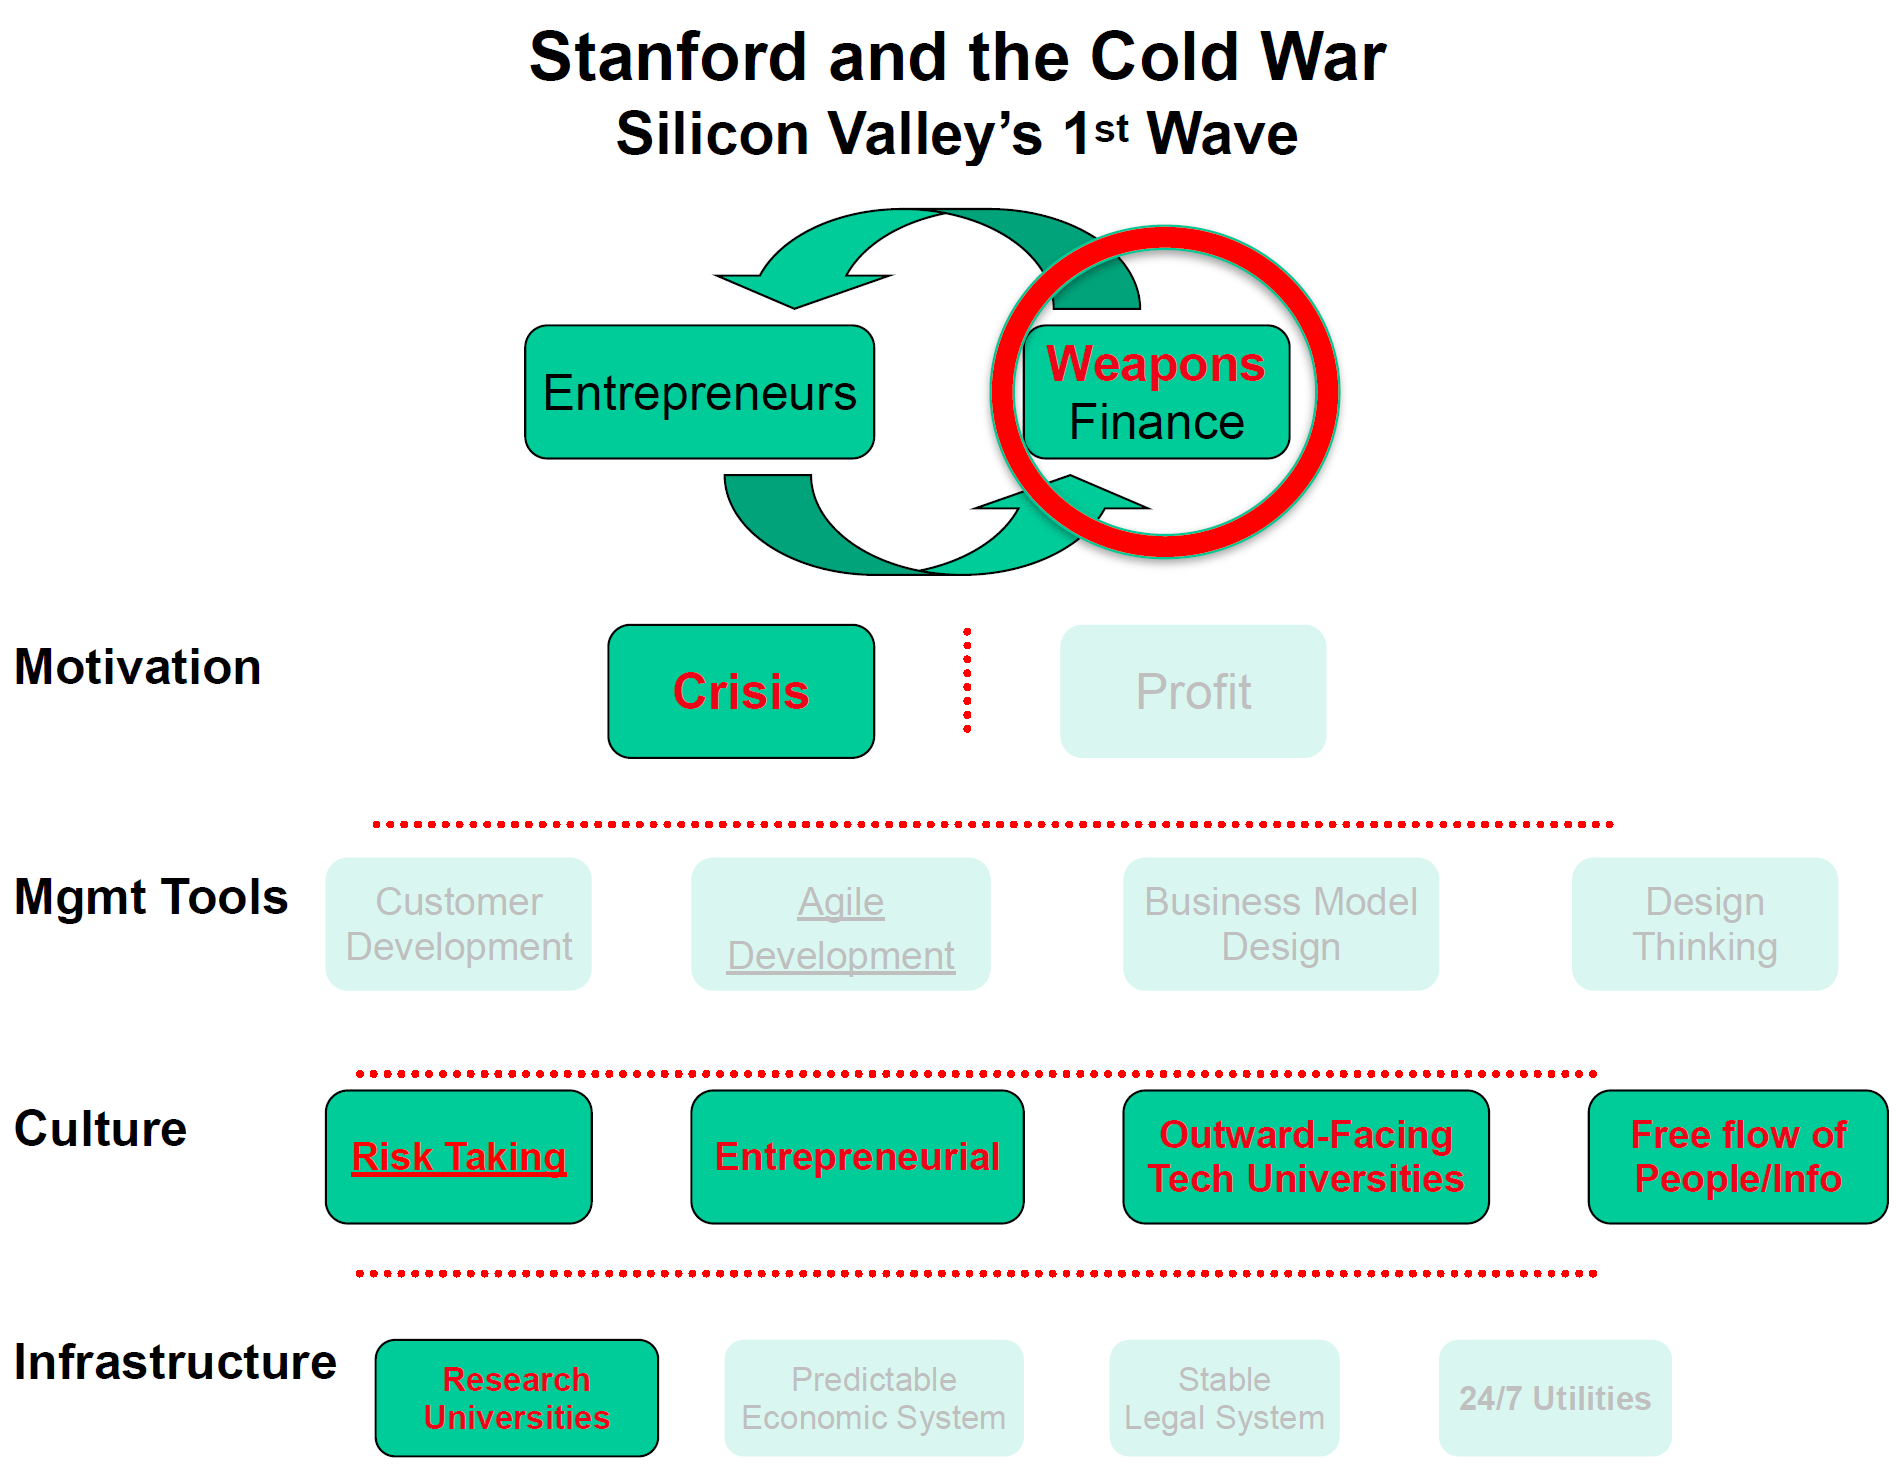
\includegraphics[width=0.7\textwidth]{Pictures/Stanford_cold_war_1.png}
\end{figure}

\begin{figure}[H]
    \centering
    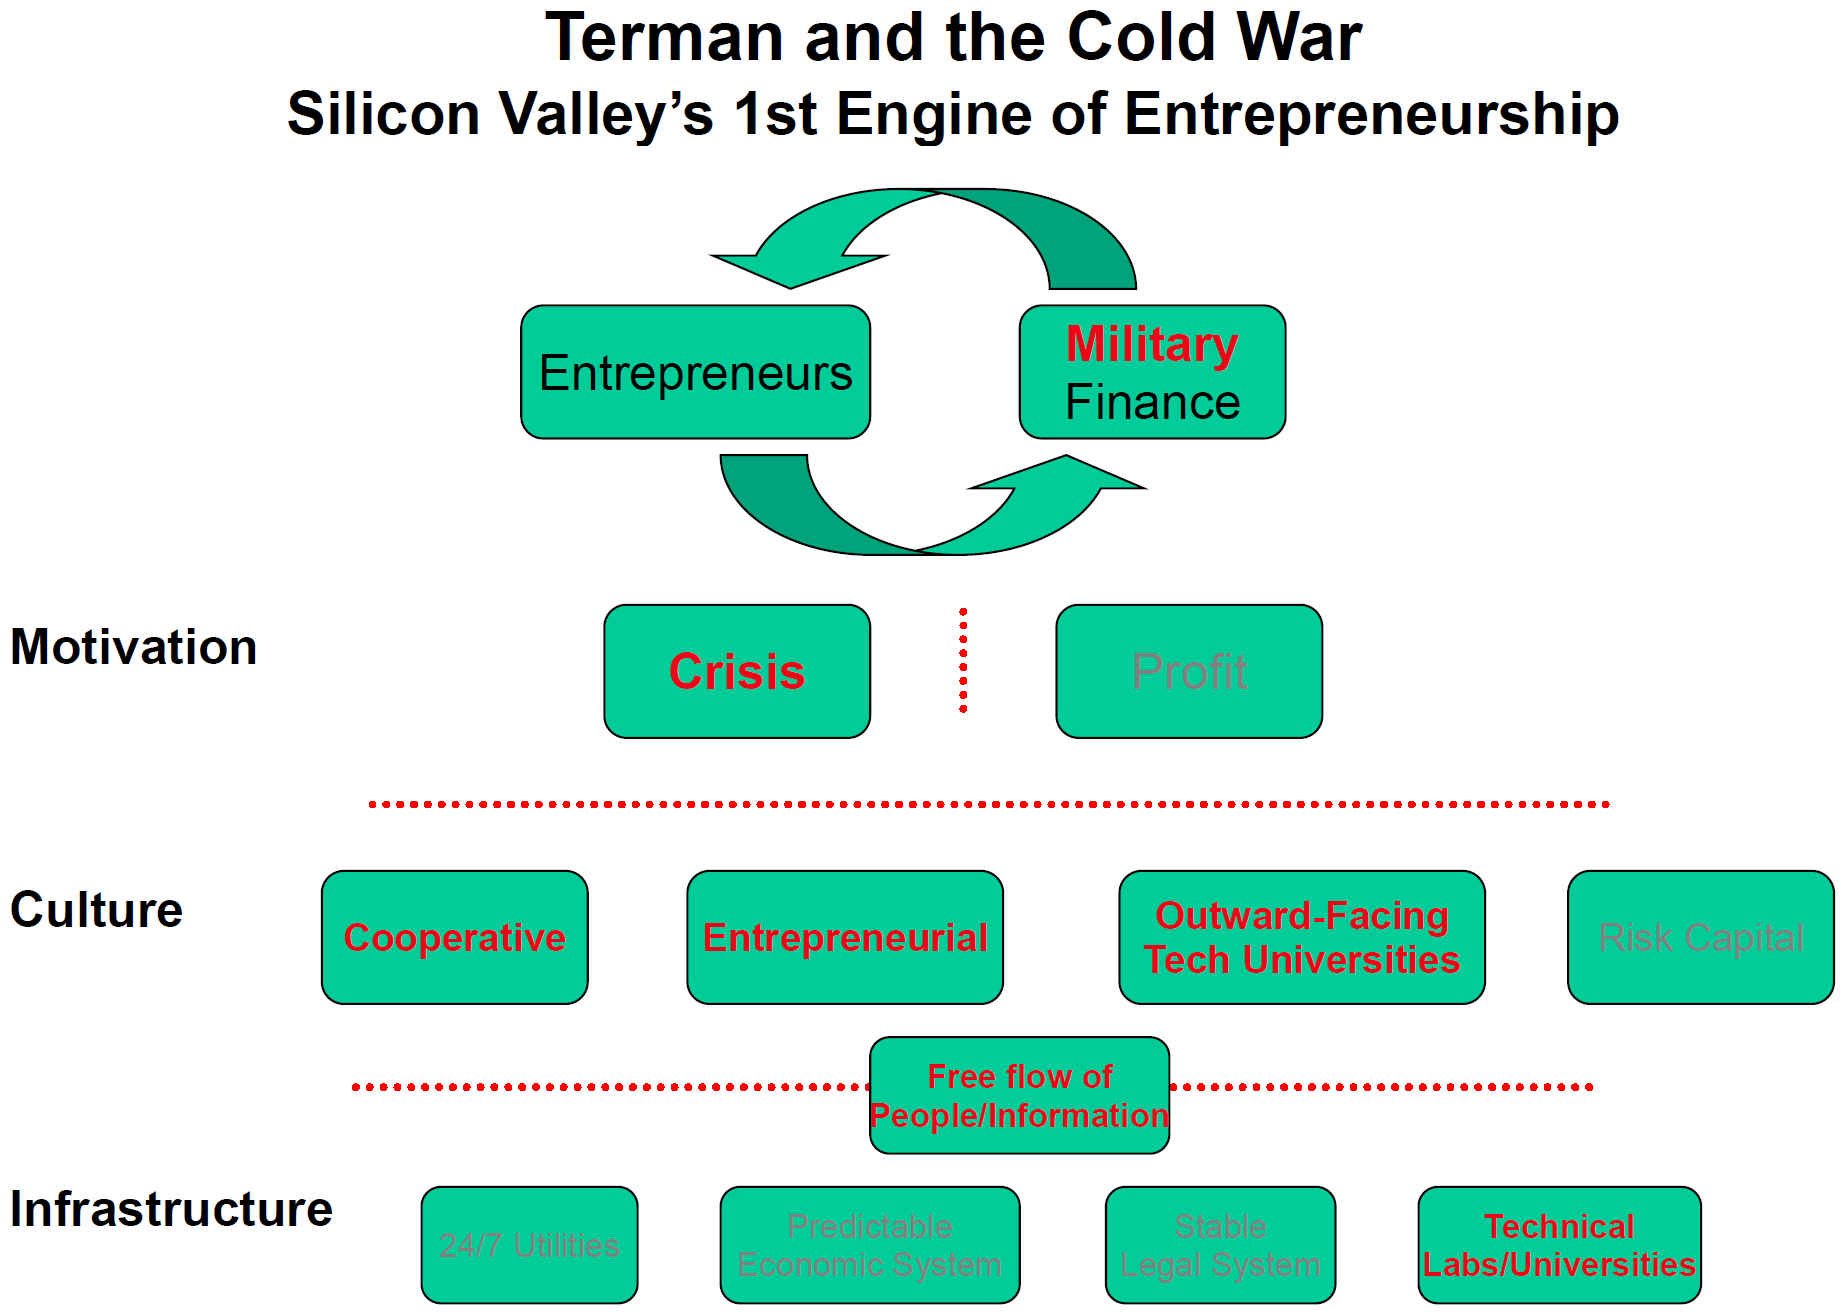
\includegraphics[width=0.7\textwidth]{Pictures/Stanford_cold_war_2.png}
\end{figure}


\paragraph{The End of Classified Work at Stanford}

\begin{itemize}
    \item In 1968, 35\% of Stanford research funding in electronics was for
        classified work
    \item 50\% of SRI's work was from DOD
    \item April 9, 1969 400 students occupy AEL
\end{itemize}

\paragraph{Shockley's Legacy}

\begin{itemize}
    \item Director of Navy anti-submarine warfare operations group at
        Columbia (1942-1943)
    \item Head of Radar Bombing training for Air Force (1943-1945)
    \item Deputy Director and Research Director of the Weapons System Evaluation
        Group in the Defense Department (1954-1955)
    \item Co-inventor of the transistor (Nobel Prize in 1956)
    \item Founded Shockley Transistor 1955
        \begin{itemize}
            \item First semiconductor company in California
        \end{itemize}
\end{itemize}

\subsubsection{The Rise of Venture Capital - The Limited Partnership}

\begin{itemize}
    \item Raise money from pension funds, private universities, wealthy
        individuals - the limited partners
    \item Investment professionals manage the fund - the general partners i.e.
        the VC's
        \begin{itemize}
            \item Compensate the general partners via the "2 and 20"
            \item 2\% management fee, 20\% carried interest (i.e. of the
                profits)
        \end{itemize}
\end{itemize}

\begin{figure}[H]
    \centering
    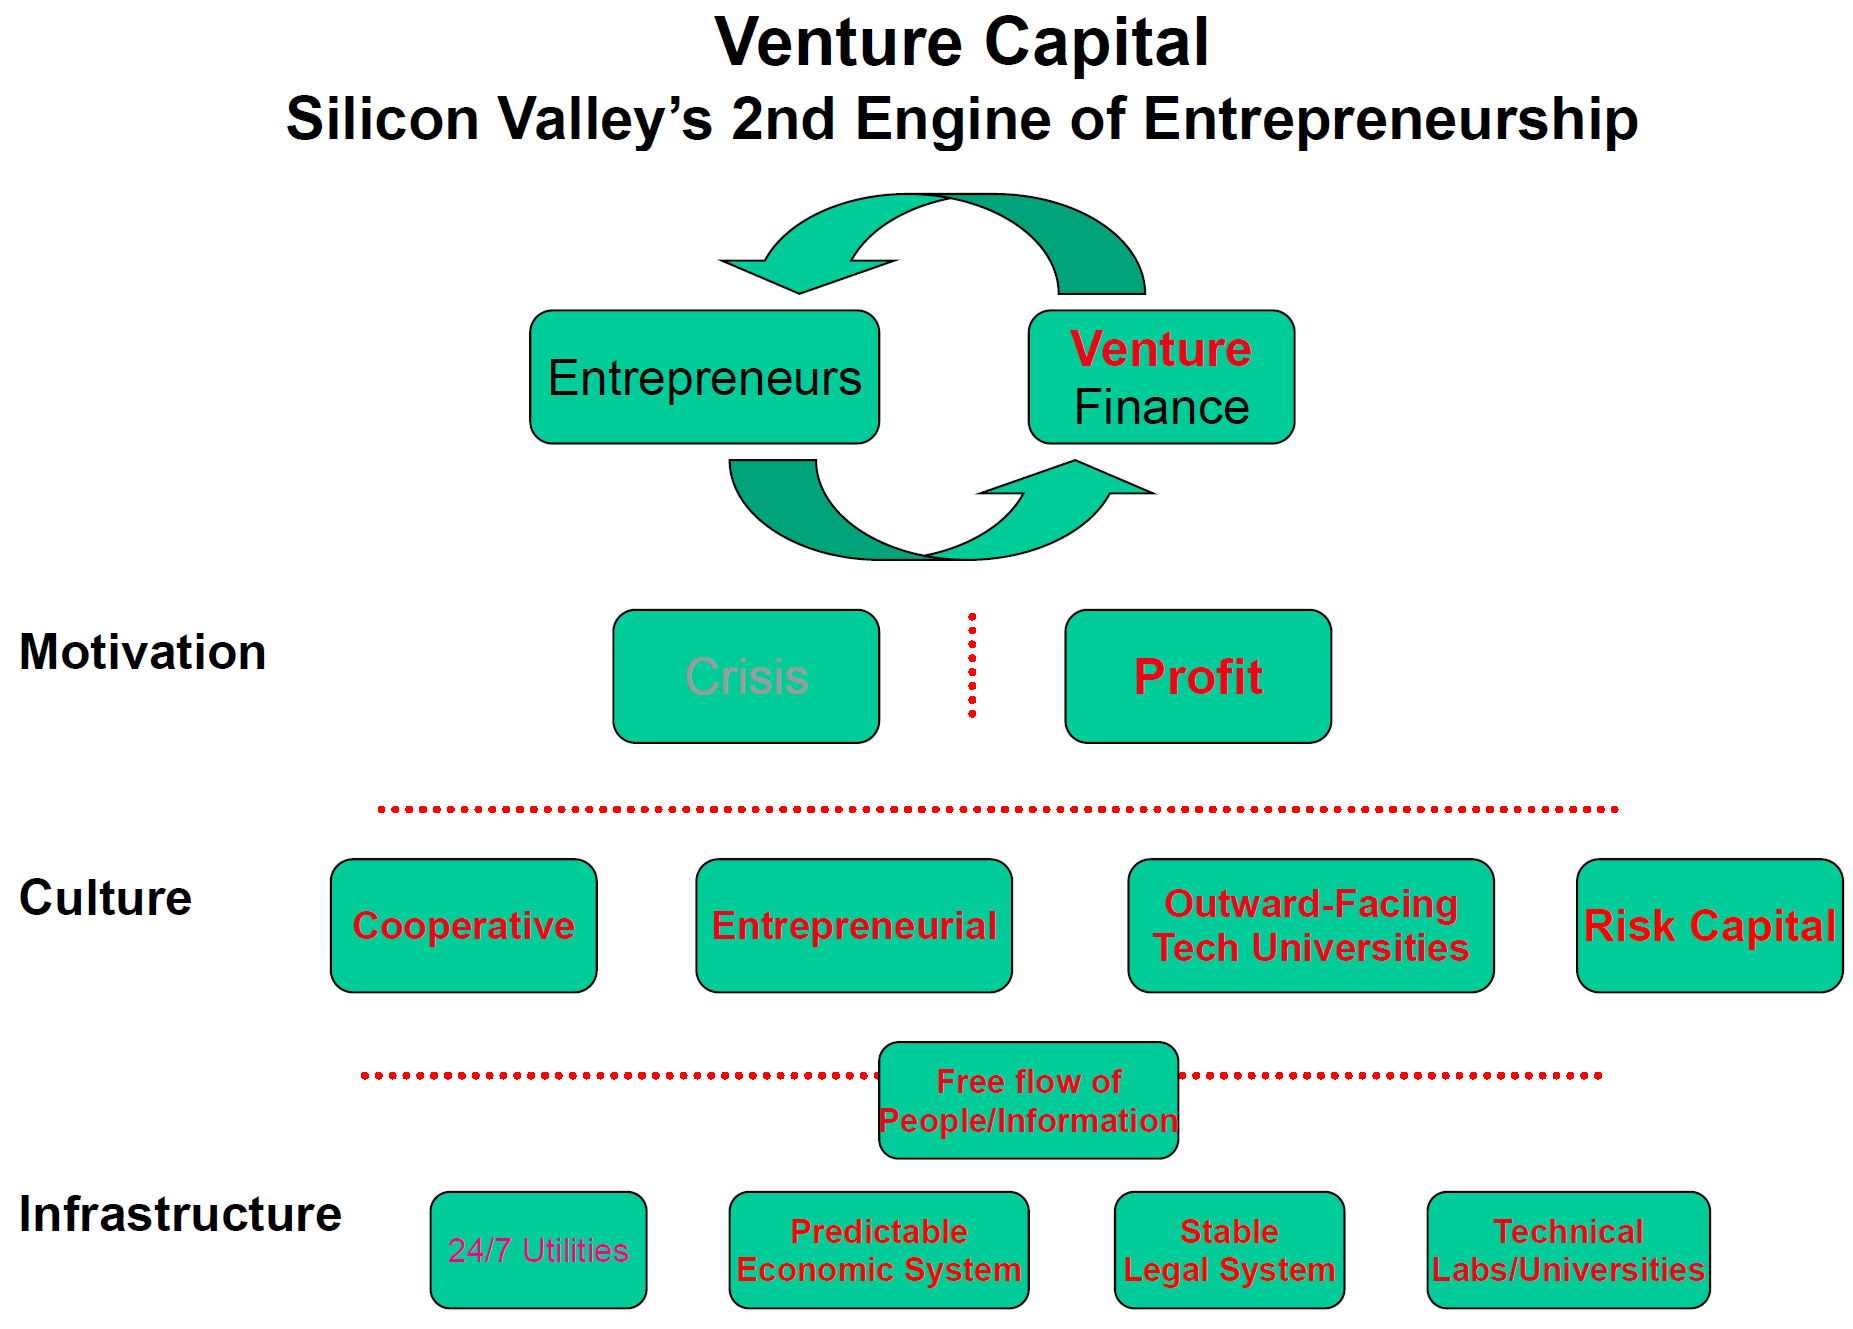
\includegraphics[width=0.8\textwidth]{Pictures/Venture_capital_silicon_valley.png}
\end{figure}

\subsubsection{Summary}

\begin{itemize}
    \item Terman/Stanford/Government responsible for entropreneurial culture
        of Silicon Valley.
    \item Military primed the pump as a customer for key Valley technologies
        \begin{itemize}
            \item Semiconductors, computers, Internet
            \item But very little technical cross pollination
        \end{itemize}
    \item Venture Capital turned the valley to volume corporate and consumer
        applications
\end{itemize}

Is there another "crisis" that will restart the valles's cycle of innovation?
Or will we continue to be profit driven?


\subsection{What is the State's role in the economy?}

\begin{enumerate}[a)]
    \item Set 'level' playing field then get out of the way
    \item solve 'market failures'
    \item something more interesting?
\end{enumerate}

The assumption: Private sector vs. public sector,
The new view: not only fixing the market but also shaping it.

Market failure policies don't explain the advent of key General Purpose
Technologies
\begin{itemize}
    \item 'mass production' system
    \item aviation technologies
    \item space technologies
    \item IT
    \item internet
    \item nuclear power
    \item nanotechnology
\end{itemize}

\begin{figure}[h]
    \centering
    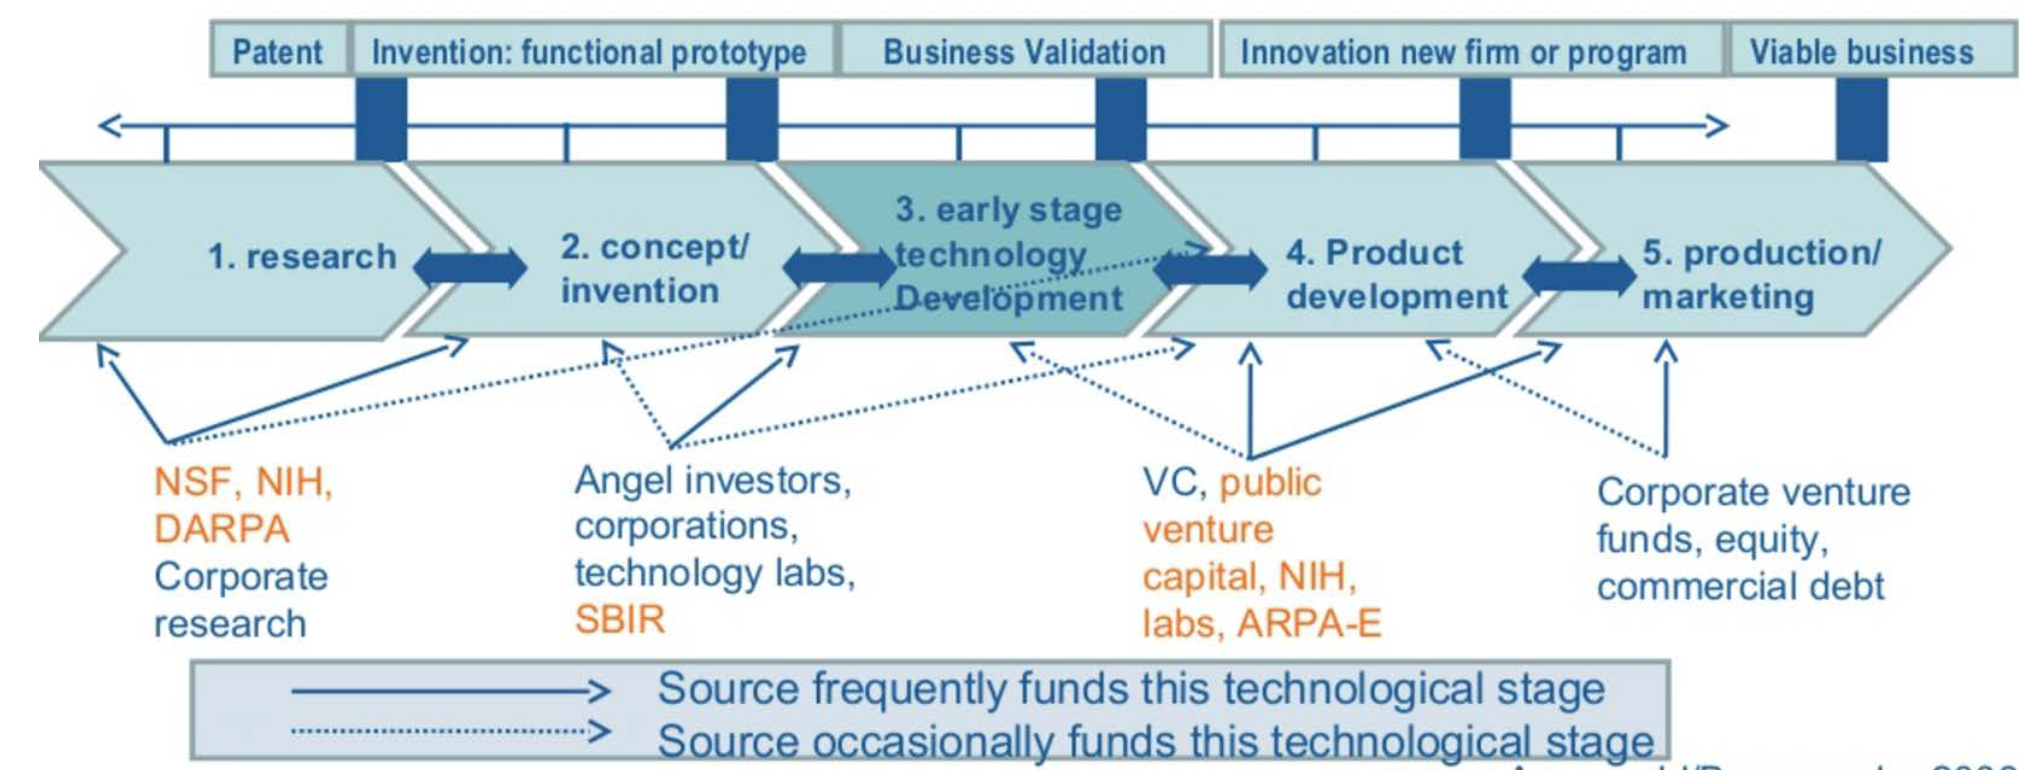
\includegraphics[width=0.7\textwidth]{Pictures/Mission_oriented_investment.png}
    \caption{Mission oriented investments along entire innovation chain}
\end{figure}

\subparagraph{Microships} powering the iPhone owe their emergense to the US
military and space programs, which made up almost the entire early market for
the breakthrough technology. In the 1960s, the government bought enough of the
initially costly chips to drive down their price 50x in a few short years,
enabling numerous new applications.

\subparagraph{Cellular communication} The early foundation of cellular
communication lies in radiotelephony capabilities advanced throughout the 20th
century with support form the US military.

\subparagraph{Internet} The technologies underpinning the Internet, which gives
the "smart phone" its smarts, were developed and funded by the Defense Department's
Advanced Research Projects Agency (DARPA) in the 1960s and 70s.

\subparagraph{GPS} was created/deployed in 1980s/90s by the military's
NAVSTAR satelite program and still today maintained via public funds.

\subparagraph{Multi-touch displays} that makes using an iPhone so intuitive has
the government's fingerprints all over it. The revolutionary interface was first
developed by a prilliant pair of universities of Delaware researchers supported
by NSF and CIA grants

\subparagraph{SIRI} was initially developed in DARPA.


\subsection{The Social Bubble Hypothesis}

"Enthusiastic supporters of an idea / a project / an opportunity weave a network
of reinforcing feedbacks based on exuberant anticipation that lead to widespread
endorsement and extraordinary commitment beyond what would be rationalized by a
standard cost-benefit analysis."

\vspace{1\baselineskip}

How to engineer useful bubbles for innovation!

\vspace{1\baselineskip}

The social Bubble Hypothesis: "innovation accelerator"

\begin{definition}
    A social bubble developing during a technological project is defined when
    several of the following symptoms are simultaneously present:
    \begin{enumerate}[(i)]
        \item strong growth of presence in the media, newspapers, books,
            blogs, gossips, cocktails\dots
        \item flow of venture capital and Wall Street investments
        \item accelerated price growth of corresponding firms trading on
            organized stock markets
        \item proliferation of venture of all kinds
    \end{enumerate}
\end{definition}

Three case studies so far: The US Apollo Program (1960-1969),
The Human Genome Project (1990-2003), The FuturICT Project (2010-2013)

\paragraph{The Human Genome Project}

\begin{itemize}
    \item In February 2001, Celera and HGP scientists published details of their
        drafts, describing the methods used and offering analysis of the
        sequence
    \item Improved drafts were announced and presented to the public in 2003,
        filling the open gaps
\end{itemize}

Anticipations of the commercial and medical applications of the HGP were highly
inflated. Today, it is acknowledged that insight into the genetic mapping and
sequencing effort is only seen as a starting point for future research in
biology and medicine. Contrary to claims during its development, the main fruits
of the Human Genome Project have been accruing to the research cummunity, and
almost nothing to medicine and the general public. But indirect technological
gains values at $>750$ Billions USD by Obama's administration.

\paragraph{Future social bubbles?}

\begin{itemize}
    \item biotech and nanotech, genomics, proteomics, personalised medicine
    \item Apps revolution (like pre-internet boom)
    \item open and big data revolution
    \item Green tech revolution
    \item Gas and oil Fracking
    \item Space frontier
    \item Ocean frontier
    \item Nuclear energy technology revolution
    \item Bitcoin
\end{itemize}

\paragraph{"Salvation and Profit": Deconstructing the Clean-Tech Bubble}

\begin{itemize}
    \item Form 2004 to 2008, a bubble formed in clean technologies, such as
        solar, biofuels, batteries, and other renewable energy sources.
    \item This clean-tech bubble can be rationalised through the lens of the
        Social Bubble Hypothesis, which holds that strong social interactions
        between enthusiastic supporters weave a network of reinforcing feedbacks
        that lead to widespread endorsement and extraordinary commitment by
        those involved.
    \item Detailed synthesis of the development of the clean-tech bubble, its
        history, and the role of venture capital and government funding in
        catalyzing it.
    \item Underlying narrative that was fueling the bubble.
    \item Evidence that the clean-tech bubble constituted an example of an
        innovation-accelerating process.
\end{itemize}

The clean-tech bubble was clearly a social bubble: the narrative of a "normal
imperative" to combat climate change and achieve "salvation", the ballooning
venture capital investments, and the massive government subsidies weaved a
network of self-reinforcing spirals that led to over-optimistic expectations,
excessive enthusiasm, and ovver-investments.

\vspace{1\baselineskip}

The question now arises whether the clean-tech bubble was - as it has been
historically the case for a number (but not all) bubbles - accelerated the
development, deployment, and diffusion of clean technologies. In other words,
did viable commercial and industrial infrastructure and products emerge after
the bust of the bubble?

\vspace{1\baselineskip}

Although the clean-tech bubble went burst, we can identify some factors that
indicate that the bubble did indeed catalyze technological progess in clean
and renewable energy technologies.

\vspace{1\baselineskip}

In essence, the clean-tech bubble of the mid-2000s catalyzed a massive decrease
in cost by excessively funding research and development in different clean-tech
sectors, such as solar or wind. While almost all of the clean-tech startups of
the last bubble failed, the clean-tech bubble, by decreasing prices and funding
innovation, massively de-resked clean and renewable energy technologies.
Solyndra, for example, failed because it was trying to merket a cutting-edge
new solar cell, which ended up being too expensive when the design costs started
to decrease. Today, solar or wind are no longer risky technologies and are now
even cost-competitive with legacy energy sources, such as gas or coal. This
decrease in costs and the elimination of technical risks of clean tech is now
catalyzing more investment opportunities, which, in turn, attracts new
entrepreneurs and investors, such as Softbank, Founders Fund, Sequoia Capital,
Y Combinator, and the two funds that were already investing in first clean-tech
boom-and-bust cycle, Kleiner Perkons and Khosla Ventures.


\subsection{Certain to Win}

\paragraph{John Boyd - USAF}
The fighter Pilot who changed the art of air warfare. Act fast and seem
unpredictable. "Forty-Second-Boyd": He was dubbed "Forty-second Boyd" for his
standing bet as an instructor pilor that, beginning from a position of
disadvantage, he could defeat any opposing pilot in air combat maneuvering
in less then forty seconds. He never lost.

\vspace{1\baselineskip}

Developed the Aerial Attack Study: After the study was declassified, foreign
pilots passing through Nellis took it home where it changed the way every air
force in the world flies and fights. Even today, more than 40 years later,
nothing substantial has been added to the Aerial Attack Study.

\vspace{1\baselineskip}

After a six-year assignment at Nellis, Boyd returned to collage for another
undergraduate degree. He went to the Georgia Institute of Technology where, one
night while studying for an exam in thermodynamics, he had the epiphany that
became his famous \textit{Energy-Maneuverability Theory}, or E-M Theory, as it
came to be known.

\vspace{1\baselineskip}

The E-M Theory changed everything that everyone thought they knew about fighter
combat. It enabled fighter pilots to evaluate their energy potential at any
altitude and at any maneuver. And, perhaps more importantly, the energy potential
of their adversary. It changed forever the way aircraft are fought in combat.

\vspace{1\baselineskip}

Boyd then used E-M as a design tool. Until E-M came along, fighter aircraft had
been designed to fly fast in a straight line or fly high to reach enemy bombers.
The F-X, which became the F-15, was the first Air Force fighter ever designed
with maneuvering specifications. Boyd was the father of the F-15, the F-16 and
the F-18.

\vspace{1\baselineskip}

America has dominated the skies for the past 30 years because of John Boyd.

\vspace{1\baselineskip}

After he retired, he developed a theory of combat that, according to Vice
President Dick Cheney who was Secretary of Defense at the time, was
responsible for America's swift and decisive victory in the Gulf war.

\begin{figure}[H]
    \centering
    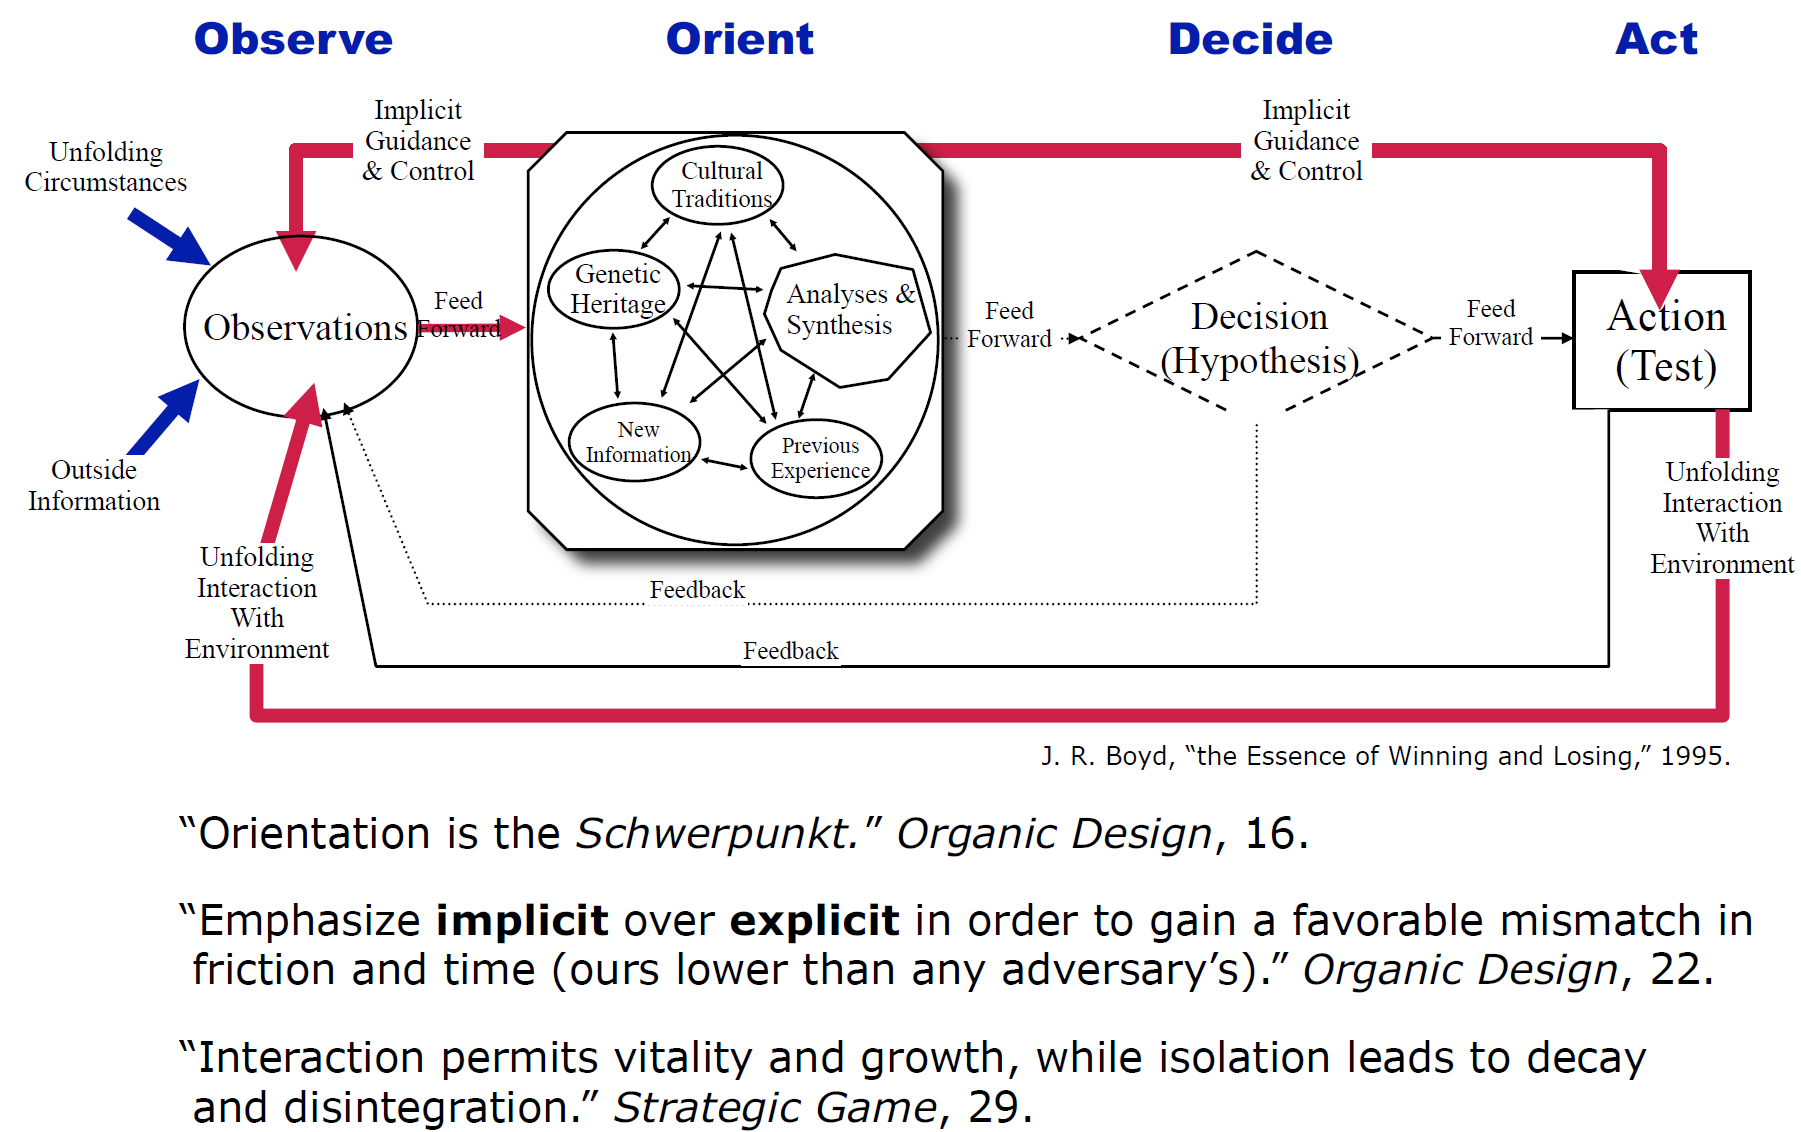
\includegraphics[width=0.8\textwidth]{Pictures/OODA.png}
\end{figure}

\begin{figure}[H]
    \centering
    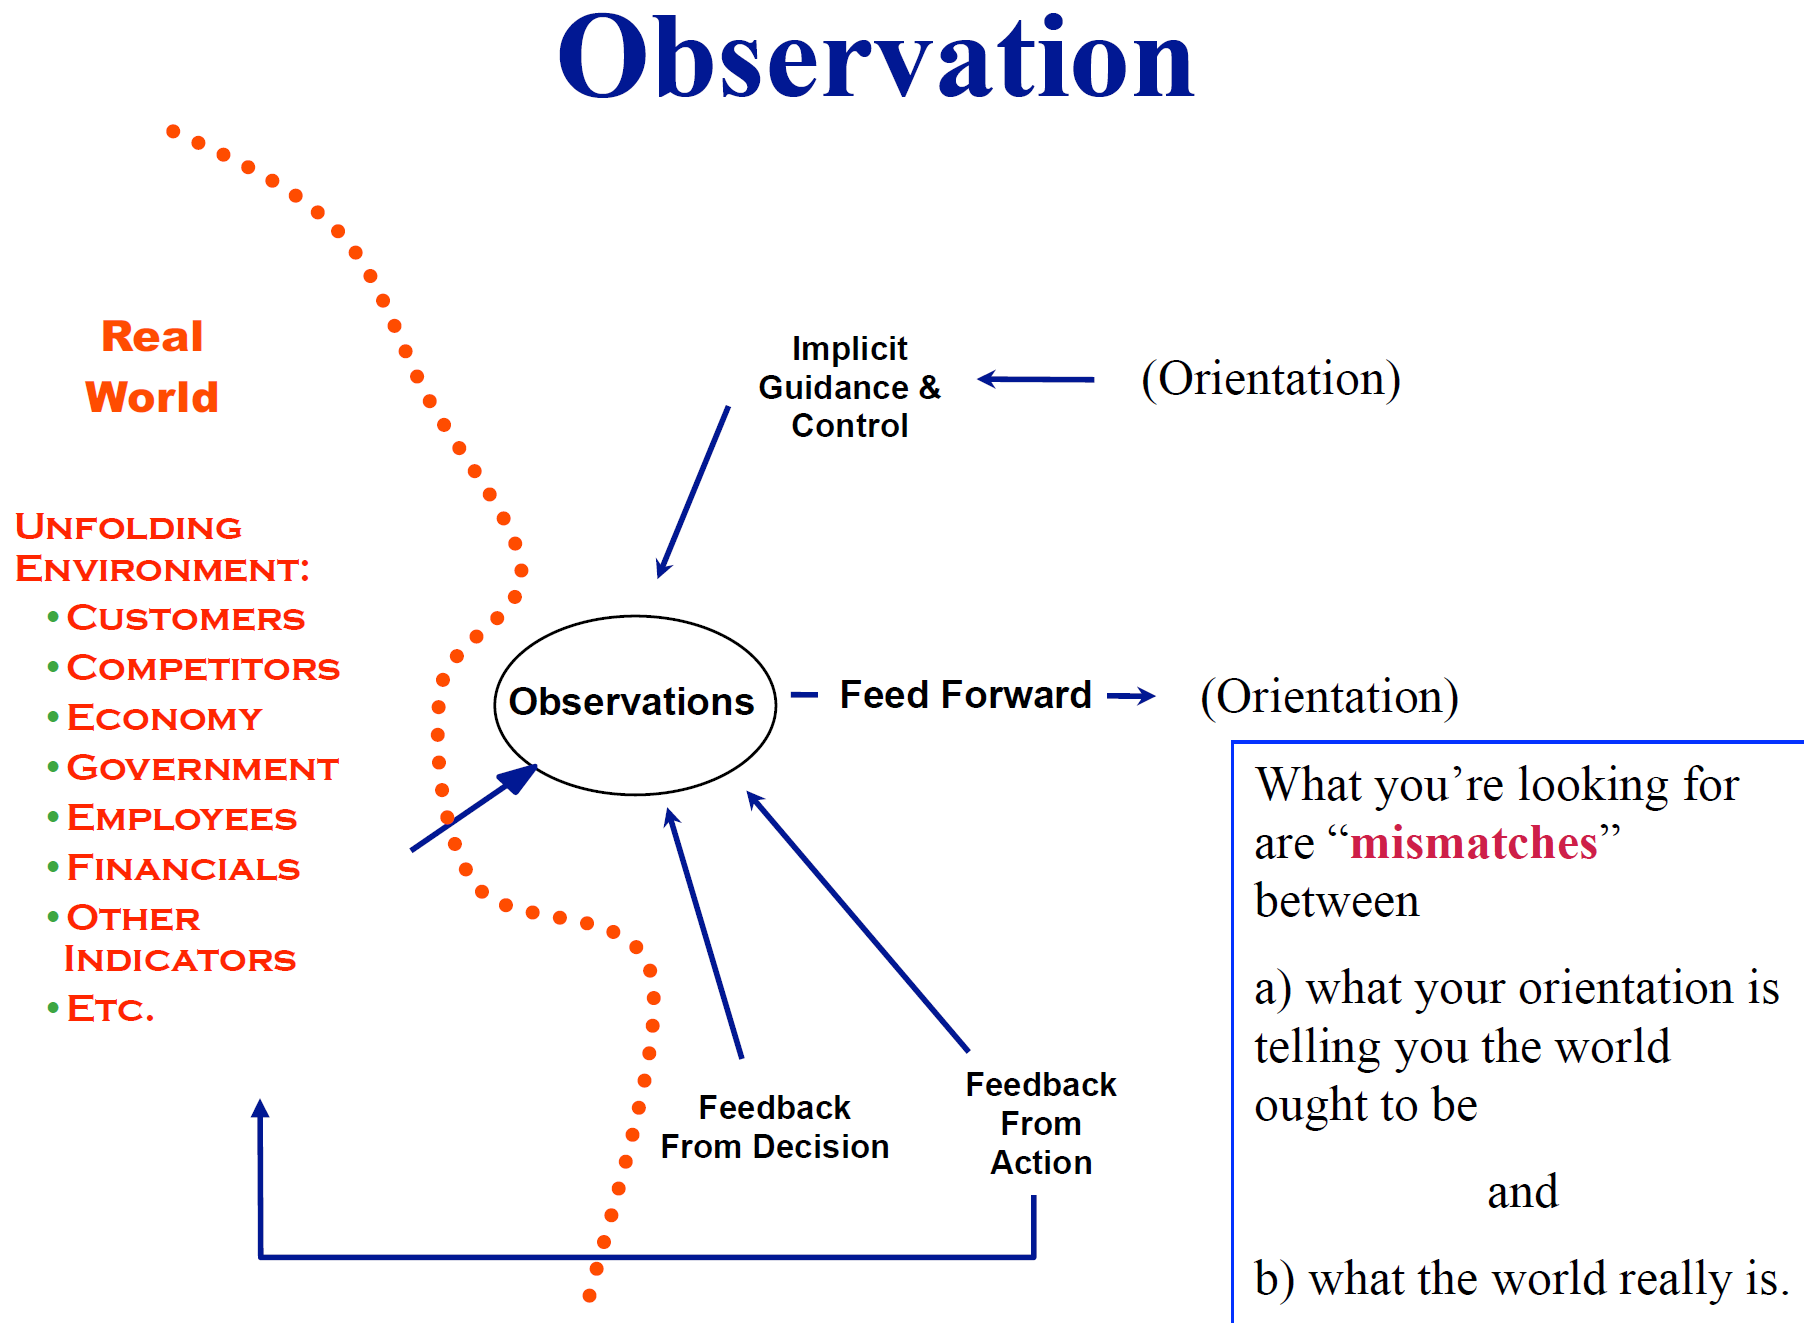
\includegraphics[width=0.7\textwidth]{Pictures/Observation.png}
\end{figure}

Wars don't always turn out as expected. Business doesn't eigher. But it's not
inevitable.

\paragraph{Time is special}

\begin{itemize}
    \item Time is the only physical parameter with a direction (the "arrow
        or time")
    \item You don't have an unlimited supply.
    \item Once it's gone, it's gone.
    \item Sure sign you're not using Boyd's strategies: you try to solve problems
        by throwing more time at them.
    \item I may lose a battle, I will never lose a minute - Napoleon
    \item A time-compressed company does the same thing as a pilot in an OODA
        loop\dots It's the competitors who act on information faster who is in
        the best position to win.
\end{itemize}

Using time as a weapon: The "H-Y War" (1981-1983)
\begin{itemize}
    \item Honda Motorcycles introduced or replaced 113 models, effectively
        turning over its entire product line twice.
    \item Yamaha, which also started about 60 models, was only able to manage
        37 changes in product line over the same 18 months.
    \item Observation: As a result, Honda was able to incorporate (and test
        in the marketplace) a much wider variety of styling \& technology. But
        that alone would not have been decisive.
\end{itemize}

Put it simple:
\begin{itemize}
    \item Good news is dangerous
    \item Bad news is the only thing that will save you, if:
        \begin{itemize}
            \item You find it before it finds you
            \item You correct your orientation
            \item You act upon it
        \end{itemize}
\end{itemize}

What determines OODA loop speed?
\begin{itemize}
    \item Ultimately, a moral climate/culture/environment that encourages
        people to use their initiatives to further the goals of the organization
    \item Under such a climate, people will solve the technical problems
\end{itemize}

Boyd's organizational climate: The principles of the Blitzkrieg
\begin{itemize}
    \item \underline{Fingerspitzengefühl} - Zen-like quality of intuitive
        understanding. Ability to sense when the time is ripe for action. Built
        through years of progressively more challenging experience.
    \item \underline{Einheit} - Has the connotation of "mutual trust" and
        implies a common outlook towards business problems. Built through common
        experience. Fingerspitzengefühl at the organizational level.
    \item \underline{Schwerpunkt} - Any concept that gives focus and direction
        to our efforts. In ambiguous situations, answers the question, "What do
        I do next?" Requires leadership.
    \item \underline{Auftragstaktik} - Tell team members what needs to be
        accomplished, get their agreement to accomplish it, then hold them
        strictly accountable for doing it - but don't prescribe how. Requires
        very high level of mutual trust.
\end{itemize}

Flowdown: Schwerpunkt for manufacturing:

The Toyota Production System, quite simply, is about shortening the time
it takes to convert customers orders into vehicle deliveries. This tells
everybody in Toyota manufacturing: "When in doubt, take the action that has
the biggest impact on order-to-delivery time".

\vspace{1\baselineskip}

Another Schwerpunkt:

Most CEOs are focused on achieving their financial and operational goals,
and on executing a strategy. But Apple's Steve Jobs believed his company's
ultimate advantage comes from its ability to make unique, or as he called
them, "insanely great" products. Jobs's entire company is focused on that
task.

\vspace{1\baselineskip}

Effective Forces play the Cheng / Ch'i Game
\begin{itemize}
    \item Sun Tzu: "Making armies able to take on opponents without being
        defeated is a matter of unorthodox (Ch'i) and orthodox (Cheng) methods\dots
        give rise to each other like a beginning-less circle - who could exhaust
        them?"
    \item Boyd: "\dots to gain a feel for the ways the cheng / ch'i game has
        been (and can be) played."
    \item Can be played on multiple levels, i.e., if opponent knows we like
        cheng / ch'i, we can exploit that fact also (Hitler at invasion of
        France, 1944)
\end{itemize}



\end{document}